\documentclass[11pt]{article}
\usepackage[margin=1in]{geometry}
\usepackage{amsmath}
\usepackage{amsthm}
\usepackage{amssymb}
\usepackage{algorithm}
\usepackage{caption}
\usepackage{subcaption}
\usepackage{color}
\usepackage[english]{babel}
\usepackage{graphicx}
\usepackage{grffile}
\usepackage{wrapfig,epsfig}
\usepackage{epstopdf}
\usepackage{url}
\usepackage{color}
\usepackage{epstopdf}
\usepackage{algpseudocode}
\usepackage{hyperref}
\usepackage[T1]{fontenc}
\usepackage{bbm}
\usepackage{comment}
\usepackage{dsfont}
\usepackage{thm-restate}
\usepackage{bm}
\usepackage{tcolorbox}
\usepackage{makecell}
\usepackage{tikz}
\usetikzlibrary{shapes,arrows.meta,positioning}




% The \author macro works with any number of authors. There are two commands
% used to separate the names and addresses of multiple authors: \And and \AND.
%
% Using \And between authors leaves it to \LaTeX{} to determine where to break
% the lines. Using \AND forces a linebreak at that point. So, if \LaTeX{}
% puts 3 of 4 authors names on the first line, and the last on the second
% line, try using \AND instead of \And before the third author name.


%\iclrfinalcopy % Uncomment for camera-ready version, but NOT for submission.










\newtheorem{theorem}{Theorem}[section]
\newtheorem*{thm}{Theorem} 
\newtheorem{lemma}[theorem]{Lemma}
\newtheorem{definition}[theorem]{Definition}
\newtheorem{notation}[theorem]{Notation}
\newtheorem{proposition}[theorem]{Proposition}
\newtheorem{corollary}[theorem]{Corollary}
\newtheorem{conjecture}[theorem]{Conjecture}
\newtheorem{assumption}[theorem]{Assumption}
\newtheorem{observation}[theorem]{Observation}
\newtheorem{fact}[theorem]{Fact}
\newtheorem{remark}[theorem]{Remark}
\newtheorem{claim}[theorem]{Claim}
\newtheorem{example}[theorem]{Example}
\newtheorem{problem}[theorem]{Problem}
\newtheorem{open}[theorem]{Open Problem}
\newtheorem{hypothesis}[theorem]{Hypothesis}
\newtheorem{question}[theorem]{Question}

\newcommand{\bvi}{\mathbf{v}^{(i)}}


\newcommand{\Tmat}{\mathcal{T}_{\mathrm{mat}}}


\newcommand{\wh}{\widehat}
\newcommand{\wt}{\widetilde}
\newcommand{\ov}{\overline}
\newcommand{\eps}{\epsilon}
\newcommand{\N}{\mathcal{N}}
\newcommand{\R}{\mathbb{R}}
\newcommand{\vol}{\mathrm{vol}}
\newcommand{\RHS}{\mathrm{RHS}}
\newcommand{\LHS}{\mathrm{LHS}}
\renewcommand{\i}{\mathbf{i}}
\renewcommand{\varepsilon}{\epsilon}
\renewcommand{\tilde}{\wt}
\renewcommand{\hat}{\wh}
\renewcommand{\bar}{\overline}
\renewcommand{\eps}{\epsilon}
\renewcommand{\d}{\mathrm{d}}
\newcommand{\norm}[1]{\left\|#1\right\|}
\newcommand{\tnabla}{\tilde{\nabla}}
\newcommand{\bx}{\mathbf{x}}
\newcommand{\ba}{\mathbf{a}}
\newcommand{\by}{\mathbf{y}}
\newcommand{\bz}{\mathbf{z}}
\newcommand{\bb}{\mathbf{b}}
\newcommand{\prox}{\mathsf{prox}}
\newcommand{\bg}{\mathbf{g}}
\newcommand{\bu}{\mathbf{u}}
\newcommand{\br}{\mathbf{r}}
\newcommand{\bc}{\mathbf{c}}
\newcommand{\bv}{\mathbf{v}}
\newcommand{\bl}{\bm{\ell}}
\newcommand{\bp}{\mathbf{p}}
\newcommand{\bh}{\mathbf{h}}
\newcommand{\boldm}{\mathbf{m}}
\newcommand{\blambda}{\bm{\lambda}}


\newcommand{\ttop}{{(t)}}
\newcommand{\ttopp}{{(t+1)}}
\newcommand{\ltop}{{(\leq t)}}



\newcommand{\bX}{\mathbf{X}}
\newcommand{\bY}{\mathbf{Y}}
\newcommand{\bZ}{\mathbf{Z}}
\newcommand{\bR}{\mathbf{R}}
\newcommand{\bS}{\mathbf{S}}
\newcommand{\bH}{\mathbf{H}}
\newcommand{\bM}{\mathbf{M}}
\newcommand{\bA}{\mathbf{A}}
\newcommand{\bN}{\mathbf{N}}
\newcommand{\bC}{\mathbf{C}}
\newcommand{\bB}{\mathbf{B}}
\newcommand{\bD}{\mathbf{D}}
\newcommand{\bG}{\mathbf{G}}
\newcommand{\bJ}{\mathbf{J}}
\newcommand{\bI}{\mathbf{I}}
\newcommand{\bU}{\mathbf{U}}
\newcommand{\bV}{\mathbf{V}}
\newcommand{\mB}{\mathcal{B}}
\newcommand{\mE}{\mathcal{E}}
\newcommand{\bW}{\mathbf{W}}
\newcommand{\bw}{\mathbf{w}}
\newcommand{\bdelta}{\boldsymbol\delta}
\newcommand{\omv}{\mathsf{OMv}}
\newcommand{\tauo}{\tau_{\mathsf{ols}}}











\DeclareMathOperator*{\E}{{\mathbb{E}}}
\DeclareMathOperator*{\Var}{{\bf {Var}}}
\DeclareMathOperator*{\Z}{\mathbb{Z}}
\DeclareMathOperator*{\C}{\mathbb{C}}
\DeclareMathOperator*{\OR}{\mathrm{OR}}
\DeclareMathOperator*{\median}{median}
\DeclareMathOperator*{\mean}{mean}
\DeclareMathOperator{\OPT}{OPT}
\DeclareMathOperator{\supp}{supp}
\DeclareMathOperator{\sparse}{sparse}
\DeclareMathOperator{\poly}{poly}
\DeclareMathOperator{\Tr}{Tr}
\DeclareMathOperator{\nnz}{nnz}
\DeclareMathOperator{\emp}{emp}
\DeclareMathOperator{\est}{est}
\DeclareMathOperator{\sparsity}{sparsity}
\DeclareMathOperator{\rank}{rank}
\DeclareMathOperator{\Diag}{diag}
\DeclareMathOperator{\dist}{dist}
\DeclareMathOperator{\dis}{dis}
\DeclareMathOperator{\signal}{signal}
\DeclareMathOperator{\cost}{cost}
\DeclareMathOperator{\vect}{vec}
\DeclareMathOperator{\tr}{tr}
\DeclareMathOperator{\RAM}{RAM}
\DeclareMathOperator{\diag}{diag}
\DeclareMathOperator{\Err}{Err}
\DeclareMathOperator{\head}{head}
\DeclareMathOperator{\tail}{tail}
\DeclareMathOperator{\cts}{cts}
\DeclareMathOperator{\jl}{jl}
\DeclareMathOperator{\new}{new}
\DeclareMathOperator{\old}{old}
\DeclareMathOperator{\refs}{ref}
\DeclareMathOperator{\im}{Im}







\renewcommand{\algorithmicrequire}{\textbf{Input:}}
\renewcommand{\algorithmicensure}{\textbf{Output:}}



\makeatletter
\newcommand*{\RN}[1]{\expandafter\@slowromancap\romannumeral #1@}
\makeatother



\title{The Complexity of Dynamic Least-Squares Regression}

% Authors must not appear in the submitted version. They should be hidden
% as long as the \iclrfinalcopy macro remains commented out below.
% Non-anonymous submissions will be rejected without review.
%\author{}
\date{}
\author{Shunhua Jiang \\ 
\vspace{.2in}
Columbia University\\ \texttt{sj3005@columbia.edu}
\and Binghui Peng \\ 
\vspace{.2in}
Columbia University\\
\texttt{bp2601@columbia.edu} 
\and Omri Weinstein\\ The Hebrew University \\  and Columbia University\\ \texttt{omri@cs.columbia.edu}
}



\begin{document}

\maketitle
%%%%%%%%%%%%%%%%%%%%%%%%%%%%%%%%%%%%%%%%%%%%%%%%%%%%%%%%%
%%%%%%%%%%%%%%%%%%%%%%%%%%%%%%%%%%%%%%%%%%%%%%%%%%%%%%%%%
\begin{abstract}
    \begin{abstract}
\label{sec:abstract}

%% 1. what is the problem 
Scientific applications that run on leadership computing facilities often face the challenge 
of being unable to fit leading science cases onto accelerator devices due to memory constraints 
(memory-bound applications).
%
% 2. what is your solution 
In this work, the authors studied one such US Department of Energy mission-critical condensed matter 
physics application, Dynamical Cluster Approximation (DCA++), and this paper discusses how device memory-bound challenges were successfully reduced  by proposing an effective 
``all-to-all'' communication method---a ring communication algorithm. 
%
This implementation takes advantage of acceleration on GPUs and remote direct memory access (RDMA) for fast data exchange between GPUs. 
%
\\Additionally, the ring algorithm was optimized with sub-ring communicators
and multi-threaded support to further reduce communication overhead and 
expose more concurrency, respectively.
%
% 3. What's the cherry-picked evaluation result you want to mention
The computation and communication were also analyzed 
by using the Autonomic Performance Environment for Exascale 
(APEX) profiling tool,  and this paper further discusses the 
performance trade-off for the ring algorithm implementation. 
%
The memory analysis on the ring algorithm shows that the allocation size for the authors' most 
memory-intensive data structure per GPU is now reduced to $1/p$ of the original size, where $p$ is the number of GPUs in the ring communicator.
%
The communication analysis suggests that 
the distributed Quantum Monte Carlo execution time grows linearly as sub-ring size increases, and the cost of messages passing through the network interface connector could be a limiting factor.


%
% \todoRed{Ronnie: Next sentence needs rewrite, too much information about Green's function that no one knows in the abstract; recommend generalizing.} \emph {However, DCA++ is currently facing memory-bound challenge as 
% a larger device array $G_t$ is limited by device memory size, where
% $G_t$ is a two-particle Green's function that allows condensed matter
% scientists to explore larger and more complex (higher fidelity)
% physics cases.}

\end{abstract}

\keywords{DCA++, Quantum Monte Carlo, GPU Remote Direct Memory Access, memory-bound issue, exascale machines}

\end{abstract}
\setcounter{page}{0}
\thispagestyle{empty}
\newpage

%%%%%%%%%%%%%%%%%%%%%%%%%%%%%%%%%%%%%%%%%%%%%%%%%%%%%%%%%
%%%%%%%%%%%%%%%%%%%%%%%%%%%%%%%%%%%%%%%%%%%%%%%%%%%%%%%%%
Reinforcement learning has achieved great success in areas such as Game-playing \citep{silver2018general,vinyals2019grandmaster}, robotics \cite{kober2013reinforcement}, large language models \citep{ouyang2022training}, etc.
However, due to safety concerns or physical limitations, in some real-world reinforcement learning problems, we must consider additional constraints that may influence the optimal policy and the learning process \citep{garcia2015comprehensive}.
% For example, a robotic arm must not take actions that may cause harm to itself or the environments.
A standard framework to handle such cases is the constrained Markov Decision Process (CMDP) \citep{altman1999constrained}.
Within the CMDP framework, the agent has to maximize
the expected cumulative reward while
obeying a finite number of constraints, which are usually in the form of expected cumulative cost criteria.

However, we are sometimes concerned with the problem with a continuum of constraints.
For example,
the constraints we meet might be time-evolving or subject to uncertain parameters, which
cannot be formulated as an ordinary CMDP
(see Examples \ref{Example_Time_Evolving} and  \ref{Example_Uncertain}).
In this paper we would study a generalized CMDP  
to address the above problem.  Because the constraints are not only infinite-number but also lie
in a continuous set,
the generalization is not trivial. Fortunately, we find that we can borrow the idea behind semi-infinite programming (SIP) \citep{remez1934determination, hettich1993semi} to deal with the semi-infinite constraints.
Accordingly, we propose \emph{semi-infinitely constrained Markov decision processes} (SICMDPs)
as a novel complement to the ordinary CMDP framework.
%More specifically,  an SICMDP model %, we consider 
%contains a continuum of constraints whereas an ordinary CMDP contains a finite number of constraints. 

%This generalization is natural but not trivial. However, we can brows the idea  
%The idea is quite natural and can be backtracked
%to the practice of extending linear programming to linear semi-infinite programming (LSIP) %\cite{remez1934determination, GobernaLSIO1998}.
%In addition, 
%As a complementary approach to the ordinary CMDP framework, 
%SICMDP can be used to model these problems  which cannot be described by a finite number of constraints
%that are not covered by .
%For example,
%the restrictions we consider can be time-evolving or subject to uncertain parameters
%, thus
%cannot be described by a finite number of constraints but a continuum of constraints 
%(see Examples \ref{Example_Time_Evolving} and  \ref{Example_Uncertain}).

We also present two reinforcement learning algorithms to solve SICMDPs called SI-CRL and SI-CPO, respectively.
SI-CRL is a model-based reinforcement learning algorithm designed for tabular cases, and SI-CPO is a policy optimization algorithm for non-tabular cases.
% and analyze its performance both theoretically and empirically.
The main challenge is that we need to deal with a continuum of constraints, thus reinforcement learning algorithms for ordinary CMDPs do not work anymore.
In SI-CRL, we tackle this difficulty by first transforming the reinforcement learning problem to an equivalent LSIP problem, which can then be solved using methods in the LSIP literature like the dual exchange methods \citep{Hu1990,reemtsen1998numerical}.
In SI-CPO, we resort to the idea of cooperative stochastic approximation developed in \cite{lan2020algorithms, wei2020comirror}.
As far as we know, we are the first to introduce tools from semi-infinitely programming (SIP) into the reinforcement learning community for solving constrained reinforcement learning problems.

% To the best of our knowledge, we are the first to apply tools from semi-infinitely programming (SIP) to solve reinforcement learning problems.
Furthermore, we give theoretical analysis for both SI-CRL and SI-CPO.
We decompose the error of SI-CRL into two parts: the statistical error from approximating the true SICMDP with an offline dataset and the optimization error due to the fact that the solution of the LSIP problem obtained by the dual exchange method is inexact.
On the optimization side, we show that the iteration complexity of SI-CRL is $O\left(\left\{\mathrm{diam}(Y)L\sqrt{|\gS|^2|\gA|m}/\left[(1-\gamma)\epsilon\right]\right\}^m\right)$.
On the statistical side, we show that the sample complexity of SI-CRL is $\widetilde O\left(\frac{|S|^2|A|^2}{\epsilon^2(1-\gamma)^3}\right)$ if the offline dataset is generated by a generative model, and $\widetilde O\left(\frac{|S||A|}{\nu_{\min} \epsilon^2(1-\gamma)^3}\right)$ if the dataset is generated by a probability measure $\nu$ as considered in \cite{chen2019information}.
Here $\widetilde O$ means that all logarithm terms are discarded.
For SI-CPO, things become a little more complicated because other than the statistical error and the optimization error, we also need to consider the function approximation error, which comes from imperfect policy parametrizations.
It is shown if the function approximation error can be controlled to $O(\epsilon)$ order, the iteration complexity of SI-CPO is $\widetilde{O}\left(\frac{1}{\epsilon^2(1-\gamma)^6}\right)$ and the sample complexity of SI-CPO is $\widetilde{O}(\frac{1}{\epsilon^4(1-\gamma)^{10}})$.
Here our iteration complexity bound is equivalent to a typical $\widetilde O(1/\sqrt{T})$ global convergence rate.

We perform a set of numerical experiments to illustrate the SICMDP model and validate our proposed algorithms.
Specifically, we examine two numerical examples, namely the discharge of sewage and ship route planning.
Through the discharge of sewage example, we show the advantage of the SICMDP framework over the CMDP baseline obtained by naive discretization in modeling realistic sequential decision-making problems.
Moreover, we demonstrate the effectiveness of the SI-CRL and SI-CPO algorithms in such tabular environments. 
In the ship route planning example, we illustrate the benefits of the SICMDP framework and the ability of the SI-CPO algorithm to address complex continuous control tasks involving continuous state spaces with modern deep reinforcement learning techniques.

% In summary, our contributions are listed as follows.
% First, we present the SICMDP model, which can be viewed as a generalization of the ordinary CMDP model.
% Second, we propose an algorithm to perform reinforcement learning for SICMDPs, which is called SI-CRL, and we believe that we are the first to apply tools from SIP
% to solve reinforcement learning problems.
% Third, we give a theoretical analysis of SI-CRL and identify both its sample complexity and iteration complexity.
% In addition, we perform numerical experiments to illustrate the SICMDP model and validate the SI-CRL algorithm.
% \{This paragraph can be removed!!! \}





\section{Technical Overview}

In this section we provide a high-level overview of Theorems \ref{thm:main_UB_informal} and \ref{thm_low_acc_LB_informal}. 

\subsection{Lower bound for fully dynamic LSR}
We start from the lower bound in Theorem \ref{thm_low_acc_LB_informal} for fully dynamic $\eps$-LSR, where we prove that  a dynamic data structure  with 
truly sub-quadratic $d^{2-\Omega(1)}$ amortized update time, even for constant approximation $\eps = 0.01$, would break the $\omv$ Conjecture. The key challenge in this proof is that the $\omv$ Conjecture itself only asserts the hardness for \emph{exact} matrix-vector products (over the boolean semiring). Our reduction proceeds in a few steps, where a key intermediate step is introducing the \emph{online projection} problem:


\begin{restatable}[Online projection]{definition}{Onlineprojection}
\label{def:online-projection} In the online projection problem, the input is a fixed orthonormal matrix $\bU \in \R^{d\times d_1}$ ($d_1\in [d]$), and a sequence of vectors $\bz^{(1)}, \ldots, \bz^{(T)}$ that arrives in an online stream. The goal is to compute the projection of $\bz^\ttop$ onto the column space of $\bU$, i.e., $\bU \bU^\top \bz^{(t)}$, at each iteration $t\in [T]$, before $\bz^{(t+1)}$ is revealed. 
\end{restatable}



For notation convenience, we write $\bz = \bz_{\bU} + \bz_{\bU_{\perp}}$ where $\bz_{\bU}$ is the projection onto $\bU$ and $\bz_{\bU_{\perp}}$ is the projection onto the orthogonal space $\bU_{\perp} \in \R^{d\times (d-d_1) }$.

\subsubsection{Hardness of online projection}
We first prove $1/\poly(d)$-hardness of online projection via reduction from $\omv$. The $\omv$ conjecture asserts the hardness of matrix-vector multiplication $(\|\bH\bz^\ttop\|)$ over Boolean semi-ring, and it is easy to see that the lower bound continues to hold when (1) the matrix $\bH$ is positive semidefinite (PSD), (2) the computation is over real, and (3) one allows $1/d^2$ error, i.e., the output $\by^\ttop$ only needs to satisfy $\|\by^\ttop - \bH\bz^\ttop\|_2 \leq O(1/d^2)$ when one normalizes $\|\bH\|_2 = 1$ and $\|\bz^\ttop\|_2 = 1$.

The online projection problem is clearly easier than arbitrary (PSD) matrix-vector multiplications, and we prove the reverse direction is also true. That is, one can (approximately) simulate a matrix-vector product with $O(\log d)$ projection queries. Given a PSD matrix $\bH$, we first perform the eigenvalue decomposition $\bH = \bU \Sigma \bU^\top$ at the preprocessing step, where $\Sigma =\diag(\lambda_1, \ldots, \lambda_d)$ is a diagonal matrix. 
We perform a {\em binary division trick} over the spectral of $\bH$. Let $S_j \subseteq [d]$ include all column indices $i\in [d]$, such that the $j$-th significant bit of $\lambda_{i}$ is non-zero. Let $\bU(j) \in \R^{d\times |S_j|}$ take columns of $\bU$ from $S_j$, then $\bH\bz^{(t)} = \sum_{j=1}^{O(\log d)}\frac{1}{2^j} \cdot \bz_{\bU(j)}^\ttop \pm O(1/d^2)$, i.e., one can obtain an $O(1/d^2)$ approximation of $\bH\bz^{(t)}$ by querying $O(\log d)$ online projection instances, with precision $O(1/d^2)$.


\subsubsection{Hardness amplification} 
Our next step is to boost the hardness of approximation from $O(1/d^2)$ to some constant. In particular, we prove the online projection problem is hard even one only needs 
$
\|\by^\ttop - \bU\bU^\top \bz^\ttop\|_2 \leq \alpha \|\bU\bU^\top \bz^\ttop\|_2 + \beta,
$
where $\alpha = 1/3$ is the multiplicative error and $\beta = 1/d^3$ is a small additive error.

Given any vector $\bz$, to obtain an $O(1/d^2)$ approximation of $\bz_{\bU}$, we set up two online projection instances, $\mathbb{P}_\bU$ and $\mathbb{P}_{\bU_{\perp}}$, and we assume $\mathbb{P}_{\bU}$ (resp.~$\mathbb{P}_{\bU_\perp}$) returns an $(\alpha,\beta)$-approximation to the projection onto $\bU$ (resp.~$\bU_{\perp}$).
A natural idea is to query $\mathbb{P}_{\bU_{\perp}}$ and obtain 
\[
\bw = \mathbb{P}_{\bU_{\perp}}(\bz) = \bz_{\bU_\perp} + \bdelta \quad \text{where the error term} \quad \|\bdelta\|_2 \leq \alpha \|\bz_{\bU_{\perp}}\|_2  + \beta.
\]
Subtracting $\bw$ and considering $\bz' = \bz - \bw$, the orthogonal component decreases by a factor of $\alpha$ (i.e., $\|\bz_{\bU_\perp}'\|_2 \leq \alpha \|\bz_{\bU_\perp}\|_2 + \beta$) and one hopes to repeat it for $O(\log d)$ times to remove the orthogonal component (almost) completely. 
However, the projection component also gets contaminated, i.e., $\bz_{\bU}' = \bz_{\bU} - \bdelta_{\bU}$. Hence, we need to further ``purify'' $\bdelta$ and ensure $\bdelta_{\bU} \approx 0$. 
We obtain it by another $O(\log d)$ iterations of refinement.\footnote{This might sound circular at a first glance because our original goal is to remove $\bz_{\bU_\perp}$ and we reduce it to remove $\bdelta_{\bU}$. The difference is that it is fine to change $\bdelta_{\bU_\perp}$ by a small multiplicative factor when removing $\bdelta_{\bU}$.}


\paragraph{Final reduction} Our final reduction proceeds in $R = O(\log d)$ rounds and each round further contains $K = O(\log d)$ iterations.
\begin{itemize}
\item {\bf Outer loop.} For each round $r \in [R]$, we wish to find $\bw_{r}$ such that  
(1) $\bw_{r}$ has a negligible component in $\bU$, i.e., $\bw_{r, \bU} \approx 0$, and  
(2) $\bw_{r}$ is $\alpha'$-approximate to $\bz_{r}$ in the direction of $\bU_{\perp}$, i.e., $\|\bw_{r, \bU_\perp} - \bz_{r, \bU_\perp}\|_2 \leq \alpha' \|\bz_{r, \bU_\perp}\|_2$ for some constant $\alpha' < 1$. 
By taking $\bz_{r+1} = \bz_{r} - \bw_{r}$, one can prove that the $\bz_{r,\bU}$ component does not change and the orthogonal component $\bz_{r, \bU_\perp}$ decreases by a factor of $\alpha'$. Repeating for $R = O(\log n)$ would be sufficient.
\item {\bf Inner loop.} Within round $r$, recall we first invoke the projection $\mathbb{P}_{\bU_{\perp}}$ and obtain  
$\bw_{r, 0} = \mathbb{P}_{\bU_{\perp}}(\bz_r)$. 
In order to remove $\bw_{r, 0, \bU}$, we query the projection $\mathbb{P}_{\bU}$ and obtain 
$\by_{r, 1} = \mathbb{P}_{\bU}(\bw_{r,0})$, and $\bw_{r, 1} = \bw_{r, 0} - \by_{r,1}$. 
We have the guarantee that $\|\bw_{r, 1, \bU}\|_2 \leq \alpha \|\bw_{r, 0, \bU}\|_2$. Repeat the above step for $K = O(\log n)$ iterations, we have $\bw_{r, K, \bU}\approx 0$. We also need to control the component in $\bU_{\perp}$. We can show that $\bw_{r, K, \bU_{\perp}} = \bw_{r, 0,\bU_{\perp}} - \sum_{k=1}^{K-1}\by_{r, k, \bU_{\perp}}$, where the second term consists of a geometric decreasing sequence with rate $\alpha$, and one has $\bw_{r, K, \bU_{\perp}} = (1 \pm O(\alpha))\bz_{r, \bU_\perp}$.
\end{itemize}

We note the above reduction is adaptive in nature, because the query depends heavily on the algorithm's previous outputs. 




\subsubsection{Reduction to fully dynamic LSR}
The final step is to reduce $(\alpha, \beta)$-online projection to fully dynamic $\eps$-LSR, with the following choice of parameters $\alpha = 1/3, \eps= 0.01$ and $\beta = 1/d^3$. A natural first attempt is to set the initial feature matrix $\bA^{(0)} = \bU_{\perp}^{\top} \in \R^{(d-d_1)\times d}$ and the labels $\mathbf{b}^{(0)} = \frac{1}{\sqrt{d}}\mathbf{1}_{d-d_1}$. This is an under-constrained linear system. Let 
$
\bx^{*} = (\bU_{\perp}\bU_{\perp}^\top)^{\dagger}\bU_{\perp}\mathbf{b}^{(0)} = \frac{1}{\sqrt{d}}\sum_{j=1}^{d-d_1}\bU_{\perp, j}
$
be the normal equation -- this is the solution with the least $\ell_2$ norm. Suppose we wish to project $\bz$ onto $\bU$, then one can insert a new row of $(\bz, 10)$ and the Normal equation becomes 
\[
\bx^{*}_{\new} = \bx^{*} +  \frac{10 - \langle \bz_{\bU_{\perp}}, \bx^{*} \rangle}{\|\bz_{\bU}\|_2^2} \bz_{\bU}.
\]
If the $\eps$-approximate solution $\bx'$ returned by the algorithm is indeed close to $\bx^{*}$, we can obtain a scaled version of $\bz_{\bU}$ by computing $\bx' - \bx^{*} \approx \bx^{*}_{\new} - \bx^{*} \propto \bz_{\bU}$. 

Unfortunately, there are infinitely many optimal solutions and an algorithm does not need to output the normal form solution.
For example, an algorithm could remember a random direction $\bv$ that is orthogonal to $\bU_{\perp}$ (at the preprocessing step) and run binary search on $\bx^{*} + \xi \cdot \bv$ to resolve the new constraint $\langle \bz , \bx \rangle = 10$. It only requires $O(d)$ time and returns an exact solution. 


\paragraph{The importance of regularization} The above issue seems to be inherent of an under-constrained linear system.
To resolve it, we consider the ridge regression instead and add a small regularization term $\lambda \|\bx\|_2$ for $\lambda = 1/d^{40}$. 
Our reduction starts with $\|\bU_{\perp}^\top \bx - \mathbf{1}_{d-d_2}\|_2 + \lambda \|\bx\|_2$, and inserts/deletes the row $(\bz , 10)$ to compute the projection of $\bz$. For ridge regression, $\bx^{*}_{\new}$ is actually not the optimal solution (instead, it is very close to the unique optimal solution) but we would prove an $\eps$-approximate solution $\bx'$ needs to be very close to $\bx_{\new}^{*}$. Therefore, one can retrieve an $(\alpha, \beta)$-approximate projection from $\bx'$ and $\bx^{*}$. 

\paragraph{Missing technical consideration} We outline a few missing details of the above argument. First, the above argument (i.e., $\bx'$ is close to $\bx^{*}_{\new}$) goes through only if $\bz_{\bU}$ is not too small (e.g., $\|\bz_{\bU}\|_2 \geq 1/d^4$). We need to efficiently test the norm $\|\bz_{\bU}\|_2$ and output $\mathbf{0}$ when it is too small. 
Second, even if $\bx_{\new}^{*}$ and $\bx'$ are close, we can only obtain a scaled version of $\bz_{\bU}$. It is not oblivious to determine the right ``scale'' because of the (constant) approximation error. Instead, we run a line search and output the minimizer of $\arg\min_{\xi}\|\bz - \xi\cdot(\bx' - \bx^{*})\|$, we prove that it gives good approximation to $\bz_{\bU}$.


\subsection{Algorithm for partially dynamic LSR}
Next we provide an overview of our algorithm in Theorem \ref{thm:main_UB_informal} for partially dynamic LSR (with row insertions only). 
Let $\boldm^\ttop = (\ba^\ttop, \beta^{(t)})$ be the $t$-th row and $\bM^\ttop$ be the input matrix that concatenates these rows.
Our approach follows the online row sampling framework \cite{clmmps15, cmp20, bdm+20}: 
When a new row arrives, we sample and keep the new row with probability (approximately) proportional to the {\em online leverage score} $\tauo^\ttop:= (\boldm^\ttop)^\top ((\bM^\ttop)^{\top} \bM^\ttop)^{-1}\boldm^\ttop$. 
We output the closed-form solution on the sampled rows: It is an $\eps$-approximate solution of LSR as long as the sampled matrix $\wt{\bM}^\ttop$ is an $\eps$-spectral approximation to the input matrix $\bM^\ttop$.


\paragraph{Warm up: oblivious adversary}
If the algorithm faces an oblivious adversary, then \cite{cmp20} proves that keeping $O(d\log(\frac{\sigma_{\max}}{\min})/\eps^2)$ rows is enough for  $\eps$-spectral approximation.
It remains to bound the computation time.
Note a direct computation of the online leverage score takes $O(d^2)$ time per row-insertion, which gives no benefit over the classic Kalman's approach. In order to accelerate this computation, we use a JL-embedding trick to compress the matrix $(\bM^\ttop)^\top\bM^\ttop$ (note a similar trick has been used in \cite{ss11, blss20}) and it reduces the computation time from $O(d^2)$ to $O(d)$ per update. 





\paragraph{Adversarial robustness of online leverage score sampling}  We need a counterpart of \cite{cmp20} for the more challenging adaptive adversary.
The recent work of \cite{bhm+21} made a first step toward adversarially robust row-sampling. However, comparing to the oblivious setting, their algorithm increases the number of sampled rows 
by a factor of $d (\frac{\sigma_{\max}}{\sigma_{\min}})^2$. Note that it has a polynomial dependence on the condition number $\frac{\sigma_{\max}}{\sigma_{\min}}$, which could be as large as $\poly(dT)$.\footnote{Indeed, if the input are drawn from isotropic Gaussian $\mathcal{N}(0, \mathbf{I}_d)$ but with one direction removed, then the condition number can be as large as $T$.}


\cite{bhm+21} considers an $\epsilon$-net over the unit vectors in $\R^d$, and for any $\bx$ in the $\epsilon$-net, they use Freedman's inequality to prove that the sampled matrix $\tilde{\bM}^{(t)}$ satisfies that $\|\tilde{\bM}^{(t)} \bx\|_2 \approx \|\bM^{(t)} \bx\|_2$ (this brings an $O(d)$ overhead using a union bound). In order to apply Freedman's inequality, they need an estimate of $\|\bM^{(t)} \bx\|_2$, which is unknown in advance since the rows of $\bM^{(t)}$ are chosen adaptively. \cite{bhm+21} directly bounds this norm by the singular values: $\sigma_{\min} \|\bx\|_2 \leq \|\bM^{(t)} \bx\|_2 \leq \sigma_{\max} \|\bx\|_2$, resulting in the additional $(\frac{\sigma_{\max}}{\sigma_{\min}})^2$ overhead. 


We provide a new analysis that overcomes this limitation. Similar to \cite{bhm+21}, we also take a union bound over the $\epsilon$-net of unit vectors $\bx \in \R^d$ to reduce to the scalar case. The key difference is that when applying Freedman's inequality, we instead consider $O(\frac{\sigma_{\min}}{\sigma_{\max}})$ truncated martingales that each guesses the correct value of $\|\bM^{(t)} \bx\|_2$, and becomes 0 once the guess becomes inaccurate. We prove that each truncated martingale concentrates according to Freedman's inequality, and since one of the guesses must be close to the true value of $\|\bM^{(t)} \bx\|_2$, taking a union bound over these $O(\frac{\sigma_{\min}}{\sigma_{\max}})$ martingales results in only an $O(\log(\frac{\sigma_{\max}}{\sigma_{\min}}))$ overhead. We believe this can also be used to improve other importance sampling schemes in \cite{bhm+21}, which we leave for future work. 

\paragraph{Robustness of JL estimation} Finally, we also need to prove the JL trick is adversarially robust. To this end, we renew the JL sketch for each sampled row. 
The sampling probability computed using the JL estimate is always an overestimate of the true online leverage score. Consequently, whenever our algorithm omits a row, the ideal algorithm using the exact online leverage scores also omits that row. This means the randomness of the JL matrix is not leaked until a new row is sampled, at which point we refresh the JL matrix.


\section{Preliminaries}

\subsection{Notation}

Let $\mX \subset \R^{I_1 \times \cdots \times I_K}$ be the space of
order-$K$ tensors, where $I_k$ denotes the dimensionality of the $k$-th
mode for $k=1,\dots,K$.  For brevity, we define
$I_{<k} := \prod_{k'<k}I_{k'}$; similarly, $I_{\leq k}, I_{k<}$ and
$I_{k \leq}$ are defined.  For a vector $Y \in \R^d$, $[Y]_i$ denotes
the $i$-th element of $Y$.  Similarly, $[X]_{i_1,\ldots,i_K}$ denotes
the $(i_1,\ldots,i_K)$ elements of a tensor $X\in\mX$. Let
$[X]_{i_1,\ldots,i_{k-1},:,i_{k+1},\ldots,i_K}$ denote an
$I_k$-dimensional vector
$(X_{i_1,\ldots,i_{k-1},j,i_{k+1},\ldots,i_K})_{j=1}^{I_k}$ called the
mode-$k$ fiber.  For a vector $Y \in \R^d$, $\|Y\| = (Y^T Y)^{1/2}$
denotes the $\ell_2$-norm and $\|Y\|_{\infty} = \max_i|[Y]_i|$ denotes
the max norm.  For tensors $X,X' \in \mX$, an inner product is defined
as
$\langle X,X' \rangle := \sum_{i_1,\ldots,i_K =1}^{I_1 \dots I_K}
X(i_1,\ldots,i_K)X'(i_1,\ldots,i_K)$
and $\|X\|_{F} = \langle X,X \rangle^{1/2}$ denotes the Frobenius
norm.  For a matrix $Z$, $\|Z\|_s := \sum_{j} \sigma_{j}(Z)$ denotes
the Schatten-1 norm, where $\sigma_j(\cdot)$ is a $j$-th singular value
of $Z$.

\subsection{Tensor Train Decomposition}

%\textit{Tensor train (TT) decomposition} is a tensor factorization
%method with a matrix product representation
%\cite{oseledets2010tt,oseledets2011tensor}.  
Let us define a tuple of positive integers $(R_1, \ldots, R_{K-1})$
and an order-$3$ tensor $G_k \in \R^{I_k \times R_{k-1} \times R_k}$
for each $k = 1,\ldots,K$.  Here, we set $R_0 = R_K = 1$.  Then, TT
decomposition represents each element of $X$ as follows:
\begin{align}
	X_{i_1,\ldots,i_K} = [G_1]_{i_1,:,:} [G_2]_{i_2,:,:} \cdots [G_K]_{i_K,:,:}. \label{eq:tt}
\end{align}
Note that $[G_k]_{i_k,:,:}$ is an $R_{k-1} \times R_k$ matrix.  We
define $\mG := \{G_k\}_{k=1}^K$ as a set of the tensors, and let $X(\mG)$
be a tensor whose elements are represented by $\mG$ as
\eqref{eq:tt}.  The tuple $(R_1, \ldots, R_{K-1})$ controls
the complexity of TT decomposition, and it is called a \textit{Tensor
  Train (TT) rank}.  Note that TT decomposition is universal, i.e.,
any tensor can be represented by TT decomposition with sufficiently
large TT rank~\cite{oseledets2010tt}.


When we evaluate the computational complexity, we assume the shape of
$\mG$ is roughly symmetric. That is, we assume there exist
$I,R\in\mathbb{N}$ such that $I_k=O(I)$ for $k=1,\dots,K$ and
$R_k=O(R)$ for $k=1,\dots,K-1$.


\subsection{Tensor Completion Problem}

Suppose there exists a true tensor $X^* \in \mX$ that is unknown, and
a part of the elements of $X^*$ is observed with some noise.  Let
$S \subset \{(j_1,j_2,
\ldots,j_K)\}_{j_1,\ldots,j_K=1}^{I_1,\ldots,I_K}$
be a set of indexes of the observed elements and
$n := |S| \leq \prod_{k=1}^K I_k$ be the number of observations.  Let
$j(i)$ be an $i$-th element of $S$ for $i=1,\ldots,n$, and $y_i$
denote $i$-th observation from $X^*$ with noise.  We consider the
following observation model:
\begin{align}
	y_i = [X^*]_{j(i)} + \epsilon_i, \label{model:obs}
\end{align}
where $\epsilon_i$ is i.i.d. noise with zero mean and variance
$\sigma^2$.  For simplicity, we introduce  observation vector
$Y := (y_1, \ldots, y_n)$, noise vector
$\mE := (\epsilon_1, \ldots , \epsilon_n)$, and rearranging operator
$\mathfrak{X} : \mX \to \mathbb{R}^n$ that randomly picks the elements of $X$.
%  $[\mathfrak{X}(X)]_i = [X]_{j(i)}$.
Then, the model \eqref{model:obs} is rewritten as follows:
\begin{align*}
	Y = \mathfrak{X}(X^*) + \mE.
\end{align*}

%%%
The goal of tensor completion is to estimate the true tensor $X^*$
from the observation vector $Y$.  Because the estimation problem is
ill-posed, we need to restrict the degree of freedom of $X^*$, such as
rank. Because the direct optimization of rank is difficult, its convex
surrogation is alternatively
used~\cite{candes2012exact,candes2010matrix, krishnamurthy2013low,
  zhang2016exact, phien2016efficient}.  For tensor
completion, the convex surrogation yields the following optimization
problem
\cite{gandy2011tensor,liu2013tensor,signoretto2011tensor,tomioka2010estimation}:
\begin{align}
	\min_{X \in \Theta} \left[ \frac{1}{2n} \|Y - \mathfrak{X}(X)\|^2 + \lambda_n \|X\|_{s^*} \right], \label{opt:general}
\end{align}
where $\Theta \subset \mX$ is a convex subset of $\mX$, 
%and
%$\Omega : \Theta \to \R_+$ is a regularization for tensors, 
$\lambda_n\geq 0$ is a regularization coefficient, and
$ \|\cdot\|_{s^*}$ is the overlapped Schatten norm defined as
$ \|X\|_{s^*} := \frac{1}{K} \sum_{k=1}^K \|\tilde{X}_{(k)}\|_s$.
Here, $\tilde{X}_{(k)}$ is the $k$-unfolding matrix defined by
concatenating the mode-$k$ fibers of $X$.  The overlapped Schatten
norm regularizes the rank of $X$ in terms of Tucker
decomposition~\cite{negahban2011estimation, tomioka2011statistical}.
Although the Tucker rank of $X^*$ is unknown in general, the convex
optimization adjusts the rank depending on $\lambda_n$.

To solve the convex problem~\eqref{opt:general}, the ADMM algorithm is often
employed~\cite{boyd2011distributed,tomioka2010estimation,
  tomioka2011statistical}.  Since the overlapped Schatten norm is not
differentiable, the ADMM algorithm avoids the differentiation of the
regularization term by alternatively minimizing the augmented
Lagrangian function iteratively.


%%% Local Variables:
%%% mode: latex
%%% TeX-master: "TTcomp_NIPS2017.tex"
%%% End:

\section{Lower bound for fully dynamic LSR}
\label{sec:fully}
In this section we prove that the fully dynamic LSR requires $\Omega(d^{2-o(1)})$ time per update to solve to constant accuracy under the $\omv$ conjecture.


\begin{theorem}[Hardness for fully dynamic LSR, formal version of Theorem \ref{thm_low_acc_LB_informal}]
\label{thm:lower-full}
Let $\gamma > 0$ be any constant. Let $d$ be the input dimension and $T = \poly(d)$ be the total number of update. Let $\eps < 0.01$ be any constant, assuming the $\omv$ conjecture is true, then any algorithm that maintains an $\eps$-approximate solution for fully dynamic least-squares regression problem requires amortized running time at least $\Omega(d^{2 -\gamma})$.
\end{theorem}



The $\omv$ conjecture was originally proposed by \cite{hkns}. In this paper, we work on the standard Word RAM model with word size $O(\log n)$.
\begin{conjecture}[$\omv$ conjecture, \cite{hkns}]
\label{conj:omv}
Let $\gamma > 0$ be any constant. Let $d$ be an integer and $T \geq d$. 
Let $\bB\in \{0,1\}^{d \times d}$ be a Boolean matrix. A sequence of Boolean vectors $\bz^{(1)}, \ldots, \bz^{(T)} \in \{0,1\}^d$ are revealed one after another, and an algorithm solves the $\omv$ problem if it returns the Boolean matrix-vector product $\bB \bz^{(t)} \in \R^d$ after receiving $\bz^\ttop$ at the $t$-th step.
The conjectures states that there is no algorithm that solves the $\omv$ problem using $\poly(d)$ preprocessing time and $O(d^{2-\gamma})$ amortized query time, and has an error probability $\leq 1/3$.
\end{conjecture}





The $\omv$ conjecture asserts the hardness of solving online Boolean matrix-vector product \emph{exactly}.
In order to prove Theorem~\ref{thm:lower-full}, it would be convenient to work with real-valued matrix-vector products. 
We prove that the same lower bound holds for (well-conditioned) PSD matrices, while allowing polynomially small error.  
The following result is a standard and its proof can be found in Appendix \ref{sec:fully-app}.
\begin{lemma}[Hardness of approximate real-valued OMv]
\label{lem:omv-real}
Let $\gamma > 0$ be any constant. Let $d$ be a sufficiently large integer, $T = \poly(d)$. 
Let $\bH\in \R^{d \times d}$ be any symmetric matrix whose eigenvalues satisfy 
$
1/3\leq \lambda_d(\bH) \leq \cdots \leq \lambda_1(\bH) \leq 1,
$
and $\bz^{(1)}, \ldots, \bz^{(T)}$ be online queries.
Assuming the $\omv$ conjecture is true, then there is no algorithm with $\poly(d)$ preprocessing time and $O(d^{2-\gamma})$ amortized running time that can return an $O(1/d^{2})$-approximate answer to $\bH \bz^{(t)}$ for all $t \in [T]$, i.e., a vector $\by^{(t)} \in \R^{d}$ s.t. $\|\by^{(t)} - \bH \bz^{(t)}\|_2 \leq O(1/d^2)$. 
\end{lemma}


The remaining proof of Theorem~\ref{thm:lower-full} proceeds in a few steps.
We introduce the online projection problem in Section \ref{sec:online-projection} and prove that the $\omv$ conjecture implies that the online projection problem requires $\Omega(d^{2-\gamma})$ amortized time to solve to $O(1/d^2)$ accuracy.
We amplify the hardness to constant accuracy in Section \ref{sec:hard-amplification}, and we reduce the online projection to fully dynamic-LSR in Section \ref{sec:reduction}. 
See an illustration of these steps in Figure~\ref{fig:fully}.

\begin{figure}[!ht]
  \centering
  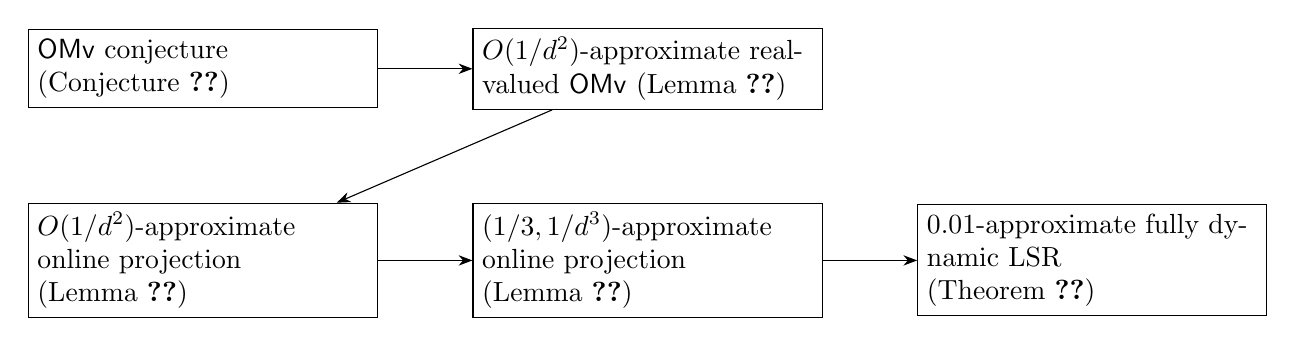
\begin{tikzpicture}[node distance=1.2cm, box/.style={rectangle, draw, text width=4.2cm}, >={Stealth[length=5pt]}]
    % Draw the nodes
    \node[box] (1) {$\omv$ conjecture \\ (Conjecture~\ref{conj:omv})};
    \node[box, right=of 1] (2) {$O(1/d^2)$-approximate real-valued $\omv$ (Lemma~\ref{lem:omv-real})};
    \node[box, below=of 1] (3) {$O(1/d^2)$-approximate online projection (Lemma~\ref{lem:online-projection})};
    \node[box, right=of 3] (4) {$(1/3, 1/d^3)$-approximate online projection (Lemma~\ref{lem:hard-amplification})};
    \node[box, right=of 4] (5) {$0.01$-approximate fully dynamic LSR \\ (Theorem~\ref{thm:lower-full})};

    % Draw the arrows
    \draw[->] (1) -- (2);
    \draw[->] (2) -- (3);
    \draw[->] (3) -- (4);
    \draw[->] (4) -- (5);
  \end{tikzpicture}
  \caption{An illustration of the chain of proofs in this section.}
  \label{fig:fully}
\end{figure}





\subsection{Hardness of online projection}
\label{sec:online-projection}

Recall the definition of the online projection task, which asks to compute the projection of a sequence of online queries $\{\bz^\ttop\}_{t\in [T]}$ onto a fixed subspace $\bU$. 



\Onlineprojection*


For any orthonormal $\bU \in \R^{d\times d_1}$, let $\bU_\perp \in \R^{d\times (d-d_1)}$ be the orthonormal matrix that spans the complementary of the column space of $\bU$, i.e., it satisfies $[\bU, \bU_\perp] \in \R^{d\times d}$ is a squared orthonormal matrix. For any vector $\bz \in \R^d$, define 
\begin{align}
\bz = \bz_{\bU} + \bz_{\bU_\perp} \quad \text{where} \quad \bz_\bU = \bU\bU^{\top}\bz \quad \text{and} \quad \bz_{\bU_\perp} = (\mathbf{I} - \bU\bU^{\top})\bz.
\end{align}
That is to say, $\bz_{\bU}$ is the projection of $\bz$ onto the subspace spanned by the columns of $\bU$, and $\bz_{\bU_{\perp}}$ is the projection of $\bz$ onto the subspace spanned by the complementary of $\bU$. In this section we also denote the projection of a vector $\bz_{k}$ as $\bz_{k, \bU}$.


We prove computing online projection requires $\Omega(d^{2-\gamma})$ amortized time assuming $\omv$.
\begin{lemma}[Hardness of online projection]
\label{lem:online-projection}
Let $\gamma > 0$ be any constant. Assuming the $\omv$ conjecture is true, then there is no algorithm with $\poly(d)$ preprocessing time and $O(d^{2-\gamma})$ amortized running time that can return an $O(1/d^2)$-approximate solution $\hat{\bz}^{\ttop}_{\bU} \in \R^d$ that satisfies $\|\hat{\bz}^{\ttop}_{\bU} - \bU\bU^{\top} \bz^{(t)}\|_2 \leq O(1/d^2)$ for the online projection problem.
\end{lemma}
\begin{proof}
By Lemma \ref{lem:omv-real}, it suffices to reduce from the $O(1/d^2)$-approximate $\omv$ problem of a real-valued PSD matrix $\bH$ with eigenvalues $1/3 \leq \lambda_d(\bH) \leq \cdots \leq \lambda_1(\bH) \leq 1$.
We apply a binary division trick and (approximately) decompose $\bH$ into $k = O(\log d)$ projection matrices $\bU(1), \ldots, \bU(k)$.
Formally, let $\bH = \bU\Sigma \bU^{\top}$ where $\bU \in \R^{d\times d}$ and $\Sigma = \diag(\lambda_1(\bH), \ldots, \lambda_n(\bH))$.
Let $\lambda_{i}(\bH) =0.\lambda_{i,1}\lambda_{i,2}\ldots$ be the binary representation of $\lambda_i$ ($i \in [n]$).
For each $j \in [k]$, let 
\[
S_j = \{i:  i\in [n], \lambda_{i, j} = 1\} \subseteq [n]
\]
be the subset of coordinates with non-zero binary value at the $j$-th bit. Let $\bU(j) = \bU_{*,S_j} \in \R^{d\times |S_j|}$ be an orthonormal matrix that takes columns from $S_j$.





We reduce an $\omv$ instance to $k$ online projection instances, and show that we can compute an $O(1/d^2)$-approximate solution to an $\omv$ query of $\bH$ by using $k$ online projection queries, one for each of the $k$ online projection instances. 
In the preprocessing step, we compute the orthonormal matrices $\bU(1), \ldots, \bU(k)$, and we let them be the initial matrices of the online projection instances. This step can be done in $O(d^3\log d)$ time. 
At the $t$-th step, given an online query $\bz^\ttop \in \R^d$ of $\omv$ with norm $\|\bz^\ttop\|_2 \leq 1$, we make one query for each instance of online projection and let $\bz_j^\ttop$ be the projection returned by the $j$-th instance.
It satisfies 
\begin{align}
\|\bz^{\ttop}_{j} - \bU(j)\bU(j)^{\top}\bz^\ttop\|_2 \leq O(1/d^2). \label{eq:online-proj-guarantee}
\end{align}
The vectors $\bz^\ttop_1, \ldots, \bz^\ttop_k$ can be computed in $k \mathcal{T} = O(\mathcal{T} \cdot \log d)$ (amortized) running time, where $\mathcal{T}$ is the runtime of the online projection algorithm. Finally, we output
\begin{align}
\by^\ttop = \sum_{j=1}^{k} \frac{1}{2^j} \cdot \bz^\ttop_j \label{eq:omv-output}
\end{align}
for the $\omv$ query.
Our goal is to prove $\by^\ttop$ is an $O(1/d^2)$-approximate solution to the $\omv$ query, i.e. 
\begin{align}\label{eq:omv_error}
\|\by^\ttop - \bH\bz^\ttop\|_2 \leq O(1/d^2).
\end{align}

To this end, we have
\begin{align}
\|\by^\ttop - \bH\bz^\ttop\|_2 = &~ \left\|\sum_{j=1}^{k} \frac{1}{2^j} \cdot \bz^\ttop_j - \bH\bz^\ttop\right\|_2 \notag \\
\leq &~  \left\|\sum_{j=1}^{k} \frac{1}{2^j} \cdot \bU(j)\bU(j)^{\top}\bz^\ttop - \bH\bz^\ttop\right\|_2 + \sum_{j=1}^{k}\frac{1}{2^j}\left\|\bU(j)\bU(j)^{\top}\bz^\ttop - \bz_j^\ttop\right\|_2 \notag \\
\leq &~ \left\|\sum_{j=1}^{k} \frac{1}{2^j} \cdot \bU(j)\bU(j)^{\top} \bz^\ttop - \bH\bz^\ttop\right\|_2 + O(1/d^2).\label{eq:online1}
\end{align}
Here the first step follows from the definition of $\by^\ttop$ in Eq.~\eqref{eq:omv-output}, the second step follows from the triangle inequality, and the last step follows from Eq.~\eqref{eq:online-proj-guarantee}.

It remains to bound the first term of RHS, and it suffices to prove $\sum_{j=1}^{k} \frac{1}{2^j} \cdot \bU(j)\bU(j)^{\top}$ is close to $\bH$. 
This holds (almost) by definition. 
Formally, let $\Sigma(j) = \frac{1}{2^j}\diag(\lambda_{1,j}, \ldots, \lambda_{d, j})$ for any $j \geq 1$. By the definition of $\bU(j)$, we have
\begin{align*}
\frac{1}{2^j} \cdot \bU(j)\bU(j)^{\top} =\bU\Sigma(j)\bU^{\top}, \quad \forall j \in [k],
\end{align*}
and therefore 
\begin{align*}
\left\|\bH - \sum_{j=1}^{k}\frac{1}{2^j} \cdot \bU(j)\bU(j)^{\top}\right\|_2 = &~ \left\| \bU \Sigma \bU^{\top} - \sum_{j=1}^{k}\bU\Sigma(j)\bU^{\top}\right\|_2 \\
= &~ \left\|\sum_{j> k} \bU\Sigma(j)\bU^{\top}\right\|_2 \leq \frac{1}{2^{k}} = O(1/d^2),
\end{align*}
where the third step follows from $\| \bU\Sigma(j)\bU^{\top} \|_2 = \frac{1}{2^j} \cdot \|\bU(j) \bU(j)^{\top}\|_2 = \frac{1}{2^j}$, and the last step follows from $k = O(\log d)$.

Plugging into Eq.~\eqref{eq:online1}, we have 
\begin{align*}
\|\by^\ttop - \bH\bz^\ttop\|_2 \leq &~\left\|\sum_{j=1}^{k} \frac{1}{2^j} \cdot \bU(j)\bU(j)^{\top}\bz^\ttop - \bH\bz^\ttop\right\|_2 + O(1/d^2)\\
\leq &~ \left\|\sum_{j=1}^{k} \frac{1}{2^j} \cdot \bU(j)\bU(j)^{\top} - \bH\right\|_2 \|\bz^\ttop\|_2  + O(1/d^2)\\
\leq &~ O(1/d^2)\cdot 1 + O(1/d^2) = O(1/d^2).
\end{align*}


In summary, the above reduction means there exist an $O(1/d^2)$-approximate $\omv$ algorithm for $\bH$ with $O(d^3 \log d)$ preprocessing time and $O(\mathcal{T} \cdot \log d)$ amortized query time. If $\mathcal{T} = O(d^{2-\gamma})$ for some constant $\gamma$, then we can solve the $O(1/d^2)$-approximate $\omv$ problem for $\bH$ in amortized $O(d^{2-\gamma} \cdot \log d)$ time, and by Lemma~\ref{lem:omv-real} this contradicts with the $\omv$ conjecture.
\end{proof}






\subsection{Hardness amplification}
\label{sec:hard-amplification}
So far we have proved an $\Omega(d^{2 - \gamma})$ lower bound of the online projection problem when it is required to output an $O(1/d^2)$-approximate answer per round. 
Our next step is to amplify this approximation precision to a constant.
We first formalize the notion of $(\alpha, \beta)$-approximate projection.

\begin{definition}[$(\alpha, \beta)$-approximate projection]
Given an orthonormal matrix $\bU \in \R^{d\times d_1}$ and a vector $\bz \in \R^{d}$, we say a vector $\by\in \R^{d}$ is an $(\alpha, \beta)$-approximate projection of $\bz$ onto $\bU$, if it satisfies 
\begin{align*}
\|\by - \bU\bU^{\top}\bz\|_2 \leq \alpha \|\bU\bU^\top \bz\|_2 + \beta\|\bz\|_2.
\end{align*}
\end{definition}
As we shall see soon, the interesting regime is $\alpha = \Theta(1)$ and $\beta = 1/\poly(d)$. The problem of online projection (Definition \ref{def:online-projection}) works well with the requirement of outputting an $(\alpha, \beta)$-approximate projection per round. 

\begin{lemma}[Hardness amplification]
\label{lem:hard-amplification}
Let $\gamma > 0$ be any constant. Let $\alpha = 1/3$ and $\beta = O(1/d^3)$.
Assuming the $\omv$ conjecture is true, then there is no algorithm with $\poly(d)$ preprocessing time and $O(d^{2-\gamma})$ amortized running time that can return an $(\alpha, \beta)$-approximate solution for the online projection problem.
\end{lemma}



The reduction is formally shown in Algorithm \ref{algo:hard-amplification}. Our goal is to show that we can answer online projection queries to $O(1/d^2)$ accuracy by using $(\alpha, \beta)$-approximate oracles. We use $\mathbb{P}_\bU, \mathbb{P}_{\bU_\perp}: \R^d \to \R^d$ to denote $(\alpha, \beta)$-approximate projection oracles whose outputs satisfy that for any vector $\bz \in \R^d$, 
(1) $\|\mathbb{P}_{\bU}(\bz) - \bz_\bU\|_2 \leq  \alpha \|\bz_\bU\|_2 + \beta \|\bz\|_2$, and 
(2) $\|\mathbb{P}_{\bU_\perp}(\bz) - \bz_{\bU_\perp}\|_2 \leq  \alpha \|\bz_{\bU_\perp}\|_2 + \beta \|\bz\|_2 $.

The reduction proceeds in $R = \Theta(\log d)$ rounds (i.e., the outer-loop on Line \ref{line:outer}), and we wish to show that each round (1) keeps the projected component $\bz_{r, \bU}$, and (2) reduces the orthogonal component $\bz_{r, \bU_\perp}$ (see Lemma \ref{lem:outer}).
In each round, the reduction first calls the approximate projection oracle onto $\bU_\perp$, which gives a good approximation to the orthogonal component $\bz_{r, \bU_\perp}$, but also has non-negligible component onto space $\bU$.
To resolve this, Algorithm \ref{algo:hard-amplification} proceeds in $K = O(\log d)$ iterations (i.e., inner loop on Line \ref{line:inner}), and in each iteration, it combines the previous output and sends it to $\mathbb{P}_{\bU}$. This process gradually purifies the component onto space $\bU$ (see Lemma \ref{lem:inner-induction}).


\begin{algorithm}[!htbp]
\caption{Hardness amplification}
\label{algo:hard-amplification}
\begin{algorithmic}[1]
\State {\bf Input:} Online query $\bz$, approximate projection oracles $\mathbb{P}_{\bU}$ and $\mathbb{P}_{\bU_\perp}$
\State $\bz_1 \leftarrow \bz$
\For{$r =1,2,\ldots, R$}\Comment{$R = O(\log d)$}\label{line:outer}
\State $\bw_{r, 0} \leftarrow \mathbb{P}_{\bU_\perp}(\bz_r)$
\For{$k=1,2,\ldots, K$}\Comment{$K = O(\log d)$} \label{line:inner}
\State $\by_{r, k} \leftarrow \mathbb{P}_{\bU}(\bw_{r, k-1})$
\State $\bw_{r, k} \leftarrow \bw_{r, k-1} - \by_{r, k} $ \label{line:w-def}
\EndFor
\State $\bz_{r+1} \leftarrow \bz_{r} - \bw_{r, K}$ \label{line:update}
\EndFor
\State \Return $\bz_{R+1}$
\end{algorithmic}
\end{algorithm}



We first state the guarantee of each outer loop. W.l.o.g., we assume $\|\bz\|_2 = 1$.
\begin{lemma}
\label{lem:outer}
For each round $r \in [R]$, we have
\begin{itemize}
\item $\|\bz_{r+1, \bU} - \bz_{r, \bU}\|_2 \leq 4(K+2)\beta$, 
\item $\|\bz_{r+1, \bU_\perp}\|_2 \leq 2\alpha \|\bz_{r, \bU_\perp}\|_2 + 4K^2\beta$, and
\item $\|\bz_{r+1}\|_2 \leq 1 + O(K^4r \beta)$.
\end{itemize}
\end{lemma}


It is useful to first understand the guarantee of the inner loops. 
At the beginning, we have the following lemma for $\bw_{r, 0}$.
\begin{lemma}
\label{lem:inner-begin}
For any round $r \in [R]$, assuming $\|\bz_r\|_2\leq 2$, then we can write 
\begin{align*}
\bw_{r, 0} = \bz_{r, \bU_\perp} - \bdelta_{r, 0} \quad \text{where} \quad \|\bdelta_{r, 0}\|_{2} \leq \alpha \|\bz_{r, \bU_{\perp}}\|_2 + 2\beta.
\end{align*}
\end{lemma}
\begin{proof}
The proof follows directly from the guarantee of $\mathbb{P}_{\bU_\perp}$. In particular, we have that 
\begin{align*}
\|\bw_{r, 0} - \bz_{r, \bU_{\perp}}\|_2 = \|\mathbb{P}_{\bU_\perp}(\bz_r) - \bz_{r, \bU_{\perp}}\|_2 \leq \alpha \|\bz_{r, \bU_{\perp}}\|_2 + \beta \|\bz_r\|_2 \leq \alpha \|\bz_{r, \bU_{\perp}}\|_2 + 2\beta,
\end{align*}
where the second step holds since $\mathbb{P}_{\bU_\perp}$ returns an $(\alpha, \beta)$ approximation over projection onto $\bU_{\perp}$ and the last step holds since $\|\bz_r\|_2 \leq 2$. 
We complete the proof here.
\end{proof}

For each iteration $k \in [K]$, we have the following lemma for the inner loop.
\begin{lemma}
\label{lem:inner-induction}
For any round $r\in [R]$ and iteration $k \in [K]$, assuming $\|\bz_r\|_2 \leq 2$, we can write
\begin{align*}
\bw_{r, k} = \bz_{r, \bU_{\perp}} - (\sum_{\tau = 0}^{k-1} \bdelta_{r, \tau, \bU_{\perp}}) - \bdelta_{r, k}, ~~~\text{and}~~
\by_{r, k} = -\bdelta_{r, k-1, \bU} + \bdelta_{r, k}, 
\end{align*}
and each $\bdelta_{r, k}$ satisfies
\begin{align*}
\|\bdelta_{r, k}\|_2 \leq \alpha \|\bdelta_{r, k-1, \bU}\|_2 + 4 \beta \quad \text{and} \quad \|\bdelta_{r, k}\|_2 \leq \alpha^{k+1}\|\bz_{r, \bU_{\perp}}\|_2 + 4(k+1)\beta.
\end{align*}
\end{lemma}
\begin{proof}
We prove the claim by induction. The base case that $\bw_{r, 0} = \bz_{r, \bU_\perp} - \bdelta_{r, 0}$ and $\|\bdelta_{r, 0}\|_{2} \leq \alpha \|\bz_{r, \bU_{\perp}}\|_2 + 2\beta$ is proved in Lemma~\ref{lem:inner-begin}. (Note that $\by_{r, 0}$ is not defined.)

Suppose the lemma statement holds for $k-1$, which means we have
\begin{align}
\bw_{r, k-1, \bU} = -\bdelta_{r, k - 1, \bU} \label{eq:inner2}
\end{align}
and
\begin{align}
\|\bw_{r, k-1}\|_2 = &~ \left\|\bz_{r, \bU_{\perp}} - (\sum_{\tau=0}^{k-2} \bdelta_{r, \tau, \bU_{\perp}}) - \bdelta_{r, k-1} \right\|_2 \notag \\
\leq &~ \|\bz_{r, \bU_{\perp}}\|_2 + (\sum_{\tau=0}^{k-2} \|\bdelta_{r, \tau, \bU_{\perp}}\|_2) + \|\bdelta_{r, k-1}\|_2 \notag \\
\leq &~ \|\bz_{r, \bU_{\perp}}\|_2 + \sum_{\tau=0}^{k-1} \|\bdelta_{r, \tau}\|_2  \notag\\
\leq &~ \sum_{\tau=0}^{k} \Big( \alpha^{\tau}\|\bz_{r, \bU_{\perp}}\|_2 + 4(\tau+1)\beta \Big) \notag \\
\leq &~ \frac{1-\alpha^{k+1}}{1-\alpha} \cdot \|\bz_{r, \bU_{\perp}}\|_2 + 4K^2\beta \leq 4, \label{eq:inner3}
\end{align}
where the second step holds from triangle inequality, the third step follows from 
\[
\|\bdelta_{r, \tau}\|_2^2 = \|\bdelta_{r, \tau, \bU} + \bdelta_{r, \tau, \bU_\perp}\|_2^2 = \|\bdelta_{r, \tau, \bU}\|_2^2 + \|\bdelta_{r, \tau, \bU_\perp}\|_2^2 \geq \|\bdelta_{r, \tau, \bU}\|_2^2,
\]
the fourth step holds from Lemma \ref{lem:inner-begin} and the induction hypothesis.
The last step follows the choice of $\alpha = 1/3, \beta = O(1/d^3)$, $K = O(\log d)$, and $\|\bz_{r, \bU_\perp}\|_2 \leq \|\bz_{r}\|_2 \leq 2$.

Now we are ready to prove that the induction hypothesis also holds for the $k$-th iteration.

{\bf Properties of $\bdelta_{r,k}$ and $\by_{r,k}$.}
We have
\begin{align}
\|\by_{r, k} + \bdelta_{r, k-1, \bU}\|_2 = &~ \|\mathbb{P}_{\bU}(\bw_{r, k-1}) + \bdelta_{r, k-1, \bU}\|_2 = \|\mathbb{P}_{\bU}(\bw_{r, k}) -  \bw_{r, k-1, \bU}\|_2\notag \\
\leq &~ \alpha\|\bw_{r, k-1, \bU}\|_2 + \beta \|\bw_{r, k-1}\|_2 = \alpha\|\bdelta_{r, k-1, \bU}\|_2 + 4\beta, \label{eq:inner4}
\end{align}
where the first step follows from the definition that $\by_{r, k} = \mathbb{P}_{\bU}(\bw_{r, k-1})$, the second step follows from Eq.~\eqref{eq:inner2}, the third step holds from the guarantee of $\mathbb{P}_{\bU}$ and the last step holds from Eq.~\eqref{eq:inner2}\eqref{eq:inner3}. 

Hence, define $\bdelta_{r, k} = \by_{r, k} + \bdelta_{r, k-1, \bU}$, from Eq.~\eqref{eq:inner4} we have that
\begin{align*}
\|\bdelta_{r, k}\|_2 \leq \alpha \|\bdelta_{r, k-1, \bU}\|_2 + 4\beta.
\end{align*}
Note that this definition of $\bdelta_{r, k}$ also gives us that
\begin{equation}\label{eq:inner_y}
\by_{r, k} = \bdelta_{r, k} - \bdelta_{r, k-1, \bU}.
\end{equation}
By induction hypothesis, we also have 
\[
\|\bdelta_{r, k}\|_2 \leq \alpha \|\bdelta_{r, k-1, \bU}\|_2 + 4\beta \leq \alpha\|\bdelta_{r, k-1}\|_2 + 4\beta \leq \alpha^{k + 1}\|\bz_{r, \bU_{\perp}}\|_2 + 4(k+1)\beta.
\]

{\bf Property of $\bw_{r,k}$.} We have
\begin{align*}
\bw_{r, k} = &~ \bw_{r, k-1} - \by_{r,k} \\
= &~ \Big( \bz_{r, \bU_{\perp}} - (\sum_{\tau=0}^{k-2} \bdelta_{r, \tau, \bU_{\perp}}) - \bdelta_{r, k-1}\Big) - \Big( \bdelta_{r, k} - \bdelta_{r, k-1, \bU} \Big)\\
= &~ \bz_{r, \bU_{\perp}} - (\sum_{\tau=0}^{k-1} \bdelta_{r, \tau, \bU_{\perp}}) - \bdelta_{r, k}.
\end{align*}
Here the first step follows from the definition of $\bw_{r, k}$ (Line \ref{line:w-def}), the second step follows from the induction hypothesis about $\bw_{r,k-1}$ and Eq.~\eqref{eq:inner_y} that we just proved. We conclude the proof here.
\end{proof}


Now we can go back to analyse the outer loops and prove Lemma \ref{lem:outer}.
\begin{proof}[Proof of Lemma \ref{lem:outer}]
Consider any round $r \in [R]$. We have
\begin{align}
\bz_{r+1} = &~ \bz_{r} - \bw_{r, K} \notag \\
= &~ \bz_{r} - \Big( \bz_{r, \bU_{\perp}} - (\sum_{\tau = 0}^{K-1} \bdelta_{r, \tau, \bU_{\perp}}) - \bdelta_{r, K} \Big) \notag \\
= &~ \bz_{r, \bU} + (\sum_{\tau = 0}^{K-1} \bdelta_{r, \tau, \bU_{\perp}}) + \bdelta_{r, K} \label{eq:outer1}
\end{align}
Here the first step follows from the update rule (Line \ref{line:update}), the second step follows from Lemma \ref{lem:inner-induction}. 

Hence, we have $\bz_{r+1, \bU} = \bz_{r, \bU} + \bdelta_{r, K, \bU}$, so for the first claim, we have
\begin{align*}
\|\bz_{r+1, \bU} - \bz_{r, \bU}\|_2 = &~ \|\bdelta_{r, K, \bU}\|_2 \leq \|\bdelta_{r, K}\|_2\\
\leq &~ \alpha^{K+1}\|\bz_{r, \bU_\perp}\|_2 + 4(K+1)\beta \leq 4(K+2)\beta.
\end{align*}
Here the third step follows from Lemma \ref{lem:inner-induction}, the last step follows from $\|\bz_{r, \bU_\perp}\|_2 \leq \|\bz_{r}\|_2 \leq 2$, and the choice of parameter that $K = O(\log d)$, $\alpha = 1/3$ and $\beta = O(1/d^3)$, so that $\alpha^K < \beta$.


For the second claim, the orthogonal component $\bz_{r+1, \bU_\perp}$ satisfies
\begin{align*}
\|\bz_{r+1, \bU_\perp}\|_2 = &~ \left\|\sum_{k=0}^{K} \bdelta_{r, k, \bU_\perp}\right\|_2 \leq \sum_{k=0}^{K}\|\bdelta_{r, k, \bU_\perp}\|_2 \leq \sum_{k=0}^{K}\|\bdelta_{r, k}\|_2 \\
\leq &~ \sum_{k=0}^{K} \Big( \alpha^{k+1}\|\bz_{r, \bU_\perp}\|_2 + 4(k+1) \beta \Big) \\
\leq &~ 2\alpha \|\bz_{r, \bU_\perp}\|_2 + 4K^2 \beta,
\end{align*}
where the first step follows from Eq.~\eqref{eq:outer1}, the second step follows from triangle inequality, the fourth step follows from Lemma \ref{lem:inner-induction}, and the last step follows from the choice of parameter that $\alpha = 1/3$.


Finally, we prove the third claim by induction on $r$. First note that in the base case where $r=0$, by definition we have $\bz_{1, \bU} = \bz$, so $\|\bz_{1, \bU}\|_2 = \|\bz\|_2 = 1$. Suppose the third claim continues to hold up to round $r-1$, for the $r$-th round, we have
\begin{align*}
\|\bz_{r+1}\|_2^2 = &~ \|\bz_{r+1, \bU_\perp}\|_2^2 + \|\bz_{r+1, \bU}\|_2^2 \\
\leq &~ \big(2\alpha \|\bz_{r, \bU_\perp}\|_2 + 4K^2\beta \big)^2 + \big(\|\bz_{r, \bU}\|_2 + 4(K+2)\beta \big)^2 \\
\leq &~ \big(\|\bz_{r, \bU_\perp}\|_2 + 4K^2\beta \big)^2 + \big(\|\bz_{r, \bU}\|_2 + 4 K^2 \beta \big)^2 \\
= &~ (\|\bz_{r, \bU_\perp}\|_2^2 + \|\bz_{r, \bU}\|_2^2) + 8 K^2 \beta \cdot (\|\bz_{r, \bU_\perp}\|_2 + \|\bz_{r, \bU}\|_2) + 32 K^4 \beta^2 \\
\leq &~ \|\bz_r\|_2^2 + 16 K^2 \beta \cdot \|\bz_r\|_2 + 32 K^4 \beta^2 \\
\leq &~ 1 + O(K^4 r \beta),
\end{align*}
where the second step follows from the first two claims that we just proved: $\|\bz_{r+1, \bU_\perp}\|_2 \leq 2\alpha \|\bz_{r, \bU_\perp}\|_2 + 4K^2\beta$, and $\|\bz_{r+1, \bU}\|_2 \leq \|\bz_{r, \bU}\|_2 + \|\bz_{r+1, \bU} - \bz_{r, \bU}\|_2 \leq \|\bz_{r, \bU}\|_2 + 4(K+2)\beta$, the third step follows from $2 \alpha < 1$ since $\alpha = 1/3$ and $K+2 < K^2$ since $K = O(\log d)$, the fifth step follows from $\|\bz_r\|_2^2 = \|\bz_{r, \bU_\perp}\|_2^2 + \|\bz_{r, \bU}\|_2^2$, and the last step follows from the induction hypothesis that $\|\bz_r\|_2 \leq 1 + O(K^4 (r-1) \beta)$, and that $K^2 \beta < K^4 \beta$ and $K^4 \beta^2 < K^4 \beta$.
\end{proof}



Now we can wrap up the reduction and prove Lemma \ref{lem:hard-amplification}.
\begin{proof}[Proof of Lemma \ref{lem:hard-amplification}]
We prove that if there is an algorithm that outputs $(\alpha, \beta)$-approximate solutions for the online projection problem in $O(d^{2-\gamma})$ amortized time, then we can use this algorithm to obtain $O(1/d^2)$-approximate solutions for the online projection problem in $O(d^{2-\gamma + o(1)})$ amortized time, and hence contradicts with Lemma~\ref{lem:online-projection}.

Given an orthonormal matrix $\bU$ and let $\bz^\ttop$ be the query at the $t$-th round of the online projection problem, then we perform the reduction shown in Algorithm \ref{algo:reduction} and its output $\bz^\ttop_{R+1}$ satisfies
\begin{align*}
\|\bz_{R+1, \bU}^\ttop - \bz_{\bU}^\ttop\|_2 = &~ \|\bz_{R+1, \bU}^\ttop - \bz_{1, \bU}^\ttop\|_2 \leq \sum_{r=1}^{R} \|\bz_{r+1, \bU}^\ttop - \bz_{r, \bU}^\ttop\|_2 \leq O(RK\beta).
\end{align*}
Here the first inequality follows from triangle inequality and the second one holds due to the first claim of Lemma \ref{lem:outer}.
Meanwhile, due to the second claim of Lemma \ref{lem:outer}, we have
\begin{align*}
\|\bz_{R+1, \bU_\perp}^\ttop\|_2 \leq (2\alpha)^{K}\|\bz_{1, \bU_\perp}^\ttop\|_2 + O(RK^2\beta) \leq O(RK^2\beta),
\end{align*}
where the second step follows from that $(2 \alpha)^K < 1/d^3$ since $K = O(\log d)$ and $\alpha = 1/3$.

Combining the above two inequalities, and since $R = O(\log d)$, $K = O(\log d)$, and $\beta = O(1/d^3)$, we obtain
\begin{align*}
\|\bz_{R+1}^\ttop - \bz_{\bU}^\ttop\|_2 \leq \|\bz_{R+1, \bU}^\ttop - \bz_{\bU}^\ttop\|_2 + \|\bz_{R+1, \bU_\perp}^\ttop\|_2 \leq O(RK\beta  + RK^2\beta) \leq O(1/d^2).
\end{align*}
That is to say, $\bz_{R+1}^\ttop$ is an $O(1/d^2)$-approximate projection of $\bz^\ttop$ onto $\bU$.


We still need to bound the runtime of the reduction. Let $\mathcal{T}$ denote the amortized query time of the $(\alpha, \beta)$-approximate oracles $\mathbb{P}_{\bU_\perp}$ and $\mathbb{P}_{\bU}$. The reduction involves $R = O(\log d)$ outer loops, with each outer loop requiring a single call to $\mathbb{P}_{\bU_\perp}$ and containing $K = O(\log d)$ inner loops. During each inner loop, a single call to $\mathbb{P}_{\bU}$ is made, and the construction of $\bw_{r,k}$ takes $O(d)$ time.

Therefore, we can conclude that the total runtime of the algorithm is bounded by $RK \cdot \mathcal{T} + O(RKd) = (\mathcal{T} + d) \cdot O(\log^2 d)$. If $\mathcal{T} = O(d^{2-\gamma})$, then we can solve the $O(1/d^2)$-approximate online projection problem in amortized $O(d^{2-\gamma} \cdot \log^2 d)$ time, and this contradicts with the $\omv$ conjecture by Lemma~\ref{lem:online-projection}. This completes the proof.
\end{proof}




As a corollary, we prove the hardness of constant approximate-$\omv$.
\begin{theorem}[Hardness of approximate-$\omv$]
\label{thm:hard-omv-approx}
Let $d$ be a sufficiently large integer and $T = \poly(d)$.
Let $\gamma > 0$ be any constant, $\alpha = 1/3$ and $\beta = O(1/d^3)$. 
Let $\bH\in \R^{d\times d}$ ($\|\bH\|_2 =1$), and $\bz^{(1)}, \ldots, \bz^{(T)}$ be online queries ($\|\bz^\ttop\|_2 = 1$).
Assuming the $\omv$ conjecture is true, then there is no algorithm with $\poly(d)$ preprocessing time and $O(d^{2-\gamma})$ amortized running time that can return an $(\alpha, \beta)$-approximate answer to $\bH\bz^\ttop$ for all $t \in [T]$, i.e., a vector $\by^\ttop$ s.t. $\|\by^\ttop - \bH\bz^\ttop\|_2 \leq \alpha \|\bH\bz^\ttop\|_2 + \beta$. This continues to hold when $\bH$ is a projection matrix.
\end{theorem}




















\subsection{Reduction from online projection to fully dynamic LSR}
\label{sec:reduction}
Finally, we provide a reduction from $(\alpha, \beta)$-approximate online projection to $\epsilon$-approximate fully dynamic LSR, where $\alpha = 1/3$, $\beta = O(1/d^3)$, and $\eps = \frac{1}{100}$. 
Given an instance of online projection with orthonormal matrix $\bU \in \R^{d \times d_1}$, we first set up the LSR problem.

\vspace{+2mm}
{\bf \noindent Setup for reduction \ \ } Let 
\begin{align*}
\bA^{(0)} = 
\left[
\begin{matrix}
\sqrt{\lambda} \cdot \mathbf{I}_d \\
(\bU_\perp)^{\top}
\end{matrix}
\right] \in \R^{(2d-d_1) \times d}  \quad \text{and} \quad \bb^{(0)} = 
\left[
\begin{matrix}
\mathbf{0}_d\\
\frac{1}{\sqrt{d}} \cdot \mathbf{1}_{d-d_1}
\end{matrix} 
\right] 
\in \R^{2d-d_1}
\end{align*}
where $\lambda = 1/d^{40}$. For convenience, we have included a notation table in Table~\ref{tab:parameters}.


\begin{table}[ht]
\centering
\begin{tabular}{|c|c|c|}
\hline
Parameter & Value & Comment \\ \hline
$\eps$ & $< 1/100$ & approximation factor of fully dynamic LSR \\ \hline
$\lambda$ & $1/d^{40}$ & coefficient of the regularization term \\ \hline
$\alpha$ & $1/3$ & approximation factor of online projection \\ \hline
\end{tabular}
\caption{Parameters used in the reduction from online projection to fully dynamic LSR}
\label{tab:parameters}
\end{table}

It would be convenient to view the first $d$ rows as a regularization term, and the (squared) loss equals to
\begin{align*}
L(\bx) := \|\bA^{(0)} \bx - \bb^{(0)}\|_2^2 = \left\|(\bU_\perp)^{\top}\bx - \frac{1}{\sqrt{d}} \cdot \mathbf{1}_{d-d_1}\right\|_2^2 + \lambda \|\bx\|_2^2.
\end{align*}
In the processing step, we also compute
\begin{equation}\label{eq:def_x*}
\bx^{*} := \frac{1}{\sqrt{d}} \sum_{j=1}^{d-d_1}\bU_{\perp,j} \in \R^d,
\end{equation}
where with a slight abuse of notation we let $\bU_{\perp, j} \in \R^d$ denote the $j$-th column of matrix $\bU_\perp$ (Hence $\bx^{*}$ also lies in the column space of $\bU_\perp$).
Overall, the preprocessing step takes at most $O(d^\omega)$ time. 


\vspace{+2mm}
{\bf \noindent Online projection query \ \ } Given an online projection query $\bz^\ttop \in \R^{d}$ of the $t$-th step, recall our goal is to find an $(\alpha, 1/d^3)$-approximate projection onto $\bU$.

The reduction is formally presented in Algorithm \ref{algo:reduction}. First, it inserts a new row of $(\frac{1}{10}\cdot \bz^\ttop, 1)$ to the matrix, and then it calls the dynamic LSR solver (Line \ref{line:regression}) to obtain an $\eps$-approximate solution $\bx^\ttop$. The final output is determined as follows: if the component $\bz_\bU^\ttop$ is already sufficiently small, then it is captured by the condition on Line \ref{line:termination}, and we can simply output $\bf{0}$. Otherwise, Algorithm \ref{algo:reduction} outputs a scaled version of $(\bx^\ttop - \bx^{*})$, where the scaling factor is determined by Eq.~\eqref{eq:interpolation}. Finally, the new row is deleted, and we return to the original setup.


\begin{algorithm}[!htbp]
\caption{Reduction: From $(\alpha, 1/d^3)$-approximate online projection to $\epsilon$-approximate dynamic LSR}
\label{algo:reduction}
\begin{algorithmic}[1]
\State Insert $(\frac{1}{10}\cdot\bz^\ttop, 1) \in \R^{d}\times \R$ \Comment{Insert a new row}
\State Call the regression solver and let $\bx^{\ttop}$ be an $\eps$-approximate solution of the square root of \label{line:regression}
\begin{align}
L^\ttop(\bx) := \left\|(\bU_{\perp})^\top\bx - \frac{1}{\sqrt{d}} \cdot \mathbf{1}_{d-d_1}\right\|_2^2 + \frac{1}{100}|\langle \bz^\ttop, \bx\rangle - 10|^2 + \lambda \|\bx\|_2^2   \label{eq:lsr-r}
\end{align}
\State $\by^\ttop \leftarrow \bx^{\ttop} - \bx^{*}$ \label{line:y-rt}
\If{$\|\by^\ttop\|_2 \geq d^3$ \textbf{or} $|10 - \langle \bz^\ttop, \bx^\ttop\rangle| \geq 200 d^4\sqrt{\lambda}$}  
\label{line:termination}
\State \Return $\hat{\bz}_\bU^\ttop \leftarrow \mathbf{0}$ 
\Else
\State \Return $\hat{\bz}_\bU^\ttop \leftarrow \xi^{*} \cdot \by^\ttop$ where \label{line:interpolation}
\begin{align}
\xi^{*} = \arg\min_{\xi} \|\bz^\ttop - \xi \cdot \by^\ttop\|_2 \label{eq:interpolation}
\end{align}
\EndIf
\State Delete the row $(\frac{1}{10}\cdot\bz^\ttop, 1)$ \Comment{Delete the new row}
\end{algorithmic}
\end{algorithm}

Intuitively, the first term $\|(\bU_{\perp})^\top\bx - \frac{1}{\sqrt{d}} \cdot \mathbf{1}_{d-d_1}\|_2^2$ of the loss $L^\ttop(\bx)$ enforces the approximate solution $\bx^{(t)}$ to satisfy that $\bx^{(t)}_{\bU_{\perp}} \approx \bx^*$ on the subspace $\bU_{\perp}$, since $\bx^*$ is the minimizer of the first term. The second term $\frac{1}{100}|\langle \bz^\ttop, \bx\rangle - 10|^2$ then enforces $\bx^{(t)}_{\bU}$ to be close to a scaled version of $\bz^{(t)}_{\bU}$. Thus, $(\bx^{(t)} - \bx^*)$ is approximately a scaled version of $\bz^{(t)}_\bU$.




Formally, our goal is to prove the following lemma.
\begin{lemma}
\label{lem:reduction-lsr}
For any $t \in [T]$, the output of Algorithm \ref{algo:reduction} satisfies
\begin{align*}
\|\hat{\bz}_{\bU}^{\ttop} - \bz_{\bU}^\ttop\|_2 \leq \alpha \|\bz_\bU^\ttop\|_2 + O(1/d^3).
\end{align*}
\end{lemma}
\begin{proof}
We will prove the lemma by considering three different cases. We first give a short summary.
\begin{itemize}
\item {\bf Case 1: $\|\bz_{\bU}^\ttop\|_2 \geq 1/d^4$.} We prove that in this case we always have $|10 - \langle \bz^\ttop, \bx^{(t)}\rangle| \geq 200 d^4\sqrt{\lambda}$, so the condition of Line~\ref{line:termination} reduces to test whether $\|\by^\ttop\|_2 \geq d^3$ or not.
\begin{itemize}
\item {\bf Case 1-1: $\|\by^\ttop\|_2 \geq d^3$.} Then the condition of Line \ref{line:termination} is satisfied and we prove $\|\bz_\bU^\ttop\|_2 \leq 1/d^3$, so it is fine to output $\hat{\bz}_\bU^\ttop = \bf{0}$.
\item {\bf Case 1-2: $\|\by^\ttop\|_2 < d^3$.} Then the condition is not satisfied, and we prove the output $\hat{\bz}_\bU^\ttop = \xi^{*} \cdot \by^\ttop$ is an $(\alpha, 1/d^3)$-approximate projection of $\bz^\ttop$. 
This is the main technical part of the proof.
\end{itemize}
\item {\bf Case 2: $\|\bz_{\bU}^\ttop\|_2 < 1/d^4$.} In this case we prove that the termination condition of Line \ref{line:termination} must be true, and therefore, the output $\bz^{\ttop} = \mathbf{0}$ is an $O(1/d^3)$-approximation of $\bz_\bU^{\ttop}$.
\end{itemize}
Before going into details of the three cases, we first define a vector
\begin{align}\label{eq:x_rt*}
\bx^{*}_{t} = \bx^{*} + \frac{10 - \langle \bz_{\bU_\perp}^\ttop,\bx^{*}\rangle}{\|\bz_{\bU}^\ttop\|_2^2} \bz_{\bU}^\ttop \in \R^d.
\end{align}
We note $\bx^{*}_{t}$ is not the optimal solution of Eq.~\eqref{eq:lsr-r}, but it gives a good upper bound of the loss. 

To understand the role of $\bx_t^{*}$, note that if $\bx^{*}_{t}$ is a good approximation of the optimal solution of Eq.~\eqref{eq:lsr-r}, then $\bx^{\ttop}$ will be close to $\bx^{*}_{t}$, so $\by^\ttop = \bx^{\ttop} - \bx^{*} \approx \bx^{*}_{t} - \bx^{*}$. As a result, $\|\by^\ttop\|_2 \approx \|\bx^{*}_{t} - \bx^{*}\|_2 = O(1/\|\bz_\bU^\ttop\|_2)$. If $\|\by^\ttop\|_2 \geq d^3$ (the first part of the termination condition on Line~\ref{line:termination}) then we have $\|\bz_{\bU}^\ttop\|_2$ is small, so $\mathbf{0}$ is a good approximation of $\bz^{\ttop}_{\bU}$. 
On the other hand, if $\bx^{*}_{t}$ is not a good approximation of the optimal solution of Eq.~\eqref{eq:lsr-r}, then this means $\|\bz_{\bU}^\ttop\|_2$ is way too small, and we can capture this by the second part of the termination condition, i.e., the second term in the objective will be large.

One can verify that $\bx^{*}_{t}$ obtains zero loss except for the third regularization term. That is, it satisfies 
\begin{align*}
\langle \bx^{*}_{t}, \bU_{\perp, j}\rangle = &~ \langle \bx^{*}, \bU_{\perp,j}\rangle = \frac{1}{\sqrt{d}}, \quad \forall j \in [d-d_1], \\
\text{and, } \langle \bx^{*}_{t}, \bz^\ttop\rangle = &~\langle \bx^{*}, \bz_{\bU_\perp}^\ttop \rangle + \frac{10 - \langle \bz_{\bU_\perp}^\ttop,\bx^{*}\rangle}{\|\bz_{\bU}^\ttop\|_2^2}\cdot \langle \bz_{\bU}^\ttop, \bz_{\bU}^\ttop\rangle = 10,
\end{align*}
where the first step of the second equation follows from $\bx^*$ is in the subspace $\bU_\perp$ so it's orthogonal to $\bz_{\bU}^\ttop$.
Consequently, we have $\|(\bU_\perp)^{\top}\bx_{t}^{*} - \frac{1}{\sqrt{d}} \cdot \mathbf{1}_{d-d_1}\|_2 = 0$ and $|\langle \bz^\ttop, \bx_{t}^{*}\rangle - 10| = 0$, so $L^\ttop(\bx_{t}^{*})$ defined in Eq.~\eqref{eq:lsr-r} satisfies
\begin{align}
L^\ttop(\bx_{t}^{*}) = \lambda\|\bx_{t}^{*}\|_2^2 
\leq \lambda \cdot \frac{(10 - \langle \bz_{\bU_\perp}^\ttop,\bx^{*}\rangle)^2}{\|\bz_{\bU}^\ttop\|_2^2} + \lambda := \lambda (\Delta_{t}^2 + 1),
\label{eq:loss}
\end{align}
Here the second step follows from the definition of $\bx_{t}^{*}$ in Eq.~\eqref{eq:x_rt*}, and that $\bx^*$ has norm $\|\bx^*\|_2 \leq 1$ and it's orthogonal to $\bz_{\bU}^\ttop$, for notational convenience in the third step we have defined
\begin{equation}\label{eq:def_Delta_rt}
\Delta_{t} := \frac{10 - \langle \bz_{\bU_\perp}^\ttop, \bx^{*}\rangle}{\|\bz_{\bU}^\ttop\|_2}.
\end{equation}


\vspace{+2mm}
{\bf \noindent Case 1 \ \ } Suppose $\|\bz_{\bU}^\ttop\|_2 \geq 1/d^4$. Since $\|\bx^{*}\|_2 \leq 1$ and $\|\bz_{\bU}^\ttop\|_2 \leq 1$, we have 
\begin{align}\label{eq:Delta_bound}
\Delta_{t} = \frac{10 - \langle \bz_{\bU_\perp}^\ttop, \bx^{*}\rangle}{\|\bz_{\bU}^\ttop\|_2} \in (9,  11d^4].
\end{align}
Therefore by Eq.~\eqref{eq:loss} we have
\begin{align*}
L^\ttop(\bx_{t}^{*}) \leq \lambda (\Delta_{t}^2 + 1) \leq \lambda \cdot (1 + 121d^8).
\end{align*}
The solution $\bx^\ttop$ is $\eps$-approximately optimal where $\eps \leq 1/100$, so
\begin{align}
L^\ttop(\bx^\ttop) \leq (1+\eps)^2 \cdot L^\ttop(\bx_{t}^*) \leq 200\lambda d^8. \label{eq:loss2}
\end{align} 
This implies that
\[
\frac{1}{100} |10 - \langle \bz^\ttop, \bx^{(t)}\rangle|^2 \leq L^\ttop(\bx^{(t)}) \leq 200 \lambda d^8.
\]
So in this case we always have $|10 - \langle \bz^\ttop, \bx^{(t)}\rangle| < 200 d^4\sqrt{\lambda}$, and this means the termination condition on Line~\ref{line:termination} is equivalent to whether $\|\by^\ttop\|_2 \geq d^3$.


We make the following claim about $\bx^\ttop$, and we defer the proof of this claim to Appendix \ref{sec:fully-app}, as it involves some detailed calculations.
\begin{claim}
\label{claim:decomposition}
Let $\bV_{t}$ be the orthonormal matrix that concatenates $\bU_\perp$ and $\bz_{\bU}^\ttop$, i.e, $\bV_{t} := [\bU_\perp, \frac{\bz_{\bU}^\ttop}{\|\bz_{\bU}^\ttop\|_2}]$. Then we have
\begin{align*}
\bU_\perp(\bU_\perp)^{\top} \bx^\ttop = &~  \bx^{*} \pm 20d^4 \sqrt{\lambda}, \\
\langle \bx^\ttop, \bz_{\bU}^\ttop\rangle = &~  10 - \langle \bz_{\bU_\perp}^\ttop,\bx^{*}\rangle \pm 200d^4 \sqrt{\lambda}, \\
\|(\mathbf{I} - \bV_{t}\bV_{t}^{\top}) \cdot \bx^\ttop\|_2 \leq &~ 2\sqrt{\eps} \cdot \Delta_{t}.
\end{align*}
\end{claim}



Using Claim \ref{claim:decomposition}, we can write $\bx^\ttop$ as
\begin{align*}
\bx^\ttop = &~ \bU_\perp (\bU_\perp)^{\top} \bx^\ttop + \frac{\langle \bx^\ttop, \bz^\ttop_{\bU} \rangle}{\|\bz^\ttop_{\bU}\|_2} \cdot \frac{\bz^\ttop_{\bU}}{\|\bz_{\bU}^\ttop\|_2} + \bz_{\perp\perp}^\ttop \\
= &~ \bx^{*} + \Delta_{t}\cdot  \frac{\bz^\ttop_{\bU}}{\|\bz_{\bU}^\ttop\|_2} + \bz_{\perp\perp}^\ttop \pm O(d^8\sqrt{\lambda}),
\end{align*}
where the first step follows from decomposing $\bx_r^\ttop$ into three parts: the component that is in subspace $\bU_\perp$, the component that is in the same direction as $\bz_{\bU}^\ttop$, and the component that is orthogonal to both $\bU_\perp$ and $\bz^\ttop_{\bU}$ which we denote as $\bz_{\perp\perp}^\ttop := (\mathbf{I} - \bV_{t}\bV_{t}^{\top}) \cdot \bx^\ttop$, the second step follows from the first and second parts of Claim~\ref{claim:decomposition} and that $\|\bz_{\bU}^\ttop\|_2 \geq 1/d^4$, and finally note that using the third part of Claim~\ref{claim:decomposition} we have 
\begin{equation}\label{eq:z_perp_perp_bound}
\|\bz_{\perp\perp}^\ttop\|_2 \leq 2\sqrt{\eps}\cdot \Delta_{t}.
\end{equation}


Consequently, we can write $\by^\ttop$ as
\begin{align}\label{eq:y_rt}
    \by^\ttop = \bx^\ttop - \bx^* = \Delta_{t}\cdot  \frac{\bz^\ttop_{\bU}}{\|\bz_{\bU}^\ttop\|_2} + \bz_{\perp\perp}^\ttop \pm O(d^8\sqrt{\lambda}).
\end{align}

We further divide into two cases based on whether $\|\by^\ttop\|_2 \geq d^3$, i.e., whether the termination condition is satisfied.

\vspace{+2mm}
{\bf \noindent Case 1-1 \ \ } Suppose $\|\by^\ttop\|_2 \geq d^3$. Then it meets the termination condition and we return $\hat{\bz}_{U}^\ttop = \mathbf{0}$. 
In this case, we have
\begin{align*}
d^3 \leq \|\by^\ttop\|_2 = &~ \left\|\Delta_{t}\cdot  \frac{\bz^\ttop_{\bU}}{\|\bz_{ \bU}^\ttop\|_2} + \bz_{\perp\perp}^\ttop\right\|_2  \pm O(d^8\sqrt{\lambda} ) \\
\leq &~\Delta_{t} + \|\bz_{\perp\perp}^\ttop\|_2 \pm O(d^8\sqrt{\lambda} ) \leq (1+2\sqrt{\eps})\Delta_{t}  \pm O(d^8\sqrt{\lambda} ),
\end{align*}
where third step follows from triangle inequality, and the last step follows from Eq.~\eqref{eq:z_perp_perp_bound}. 
Since $\lambda = 1/d^{40}$ and $\eps = 1/100$, we conclude that
\begin{align*}
\frac{1}{2}d^3 \leq \Delta_{t} =  \frac{10 - \langle \bz_{\bU_\perp}^\ttop,\bx^{*}\rangle}{\|\bz_{ \bU}^{(t)}\|_2}
\leq \frac{11}{\|\bz_{\bU}^{(t)}\|_2},
\end{align*}
and therefore, $\|\bz_{\bU}^\ttop\|_2 \leq O(1/d^3)$ and it is fine to return $\hat{\bz}_{\bU}^\ttop = \mathbf{0}$.


\vspace{+2mm}
{\bf \noindent Case 1-2 \ \ } 
Suppose $\|\by^\ttop\|_2 < d^3$. Then the termination condition is not met. 
To compute $\hat{\bz}_\bU^\ttop$, we need to solve Eq.~\eqref{eq:interpolation}. Define $\xi  = \Delta_{t}^{-1} \cdot \|\bz_{\bU}^\ttop\|_2$, and we have
\begin{align}
\|\bz^\ttop - \xi \by^\ttop\|_2^2 = &~ \Big\|\bz_{\bU_\perp}^\ttop - \Delta_{t}^{-1} \cdot \|\bz_{\bU}^\ttop\|_2 \cdot \big( \bz_{\perp\perp}^\ttop \pm O(d^{8}\sqrt{\lambda}) \big) \Big\|_2^2\notag \\
= &~ \|\bz_{\bU_\perp}^\ttop\|_2^2 + \Delta_{t}^{-2} \cdot \|\bz_{\bU}^\ttop\|_2^2 \cdot \|\bz_{\perp\perp}^\ttop\|_2^2 \pm O(d^{8}\sqrt{\lambda}) \label{eq:ub1}.
\end{align}
The first step follows from Eq.~\eqref{eq:y_rt} and $\bz^\ttop = \bz_{\bU}^\ttop + \bz_{ \bU_{\perp}}^\ttop$, the second step holds since $\bz_{\bU_\perp}^\ttop$ is orthogonal to $\bz_{ \perp\perp}^\ttop$, and the error term is still $\pm O(d^8 \sqrt{\lambda})$ since $\|\bz_{\bU}^\ttop\|_2, \|\bz_{\bU_{\perp}}^\ttop\|_2, \|\bz_{\perp\perp}^\ttop\|_2 \leq 1$ and $\Delta_{t} \geq 9$ (Eq.~\eqref{eq:Delta_bound}). 


The optimal solution to Eq.~\eqref{eq:interpolation}, denoted as $\xi^{*}$, can be expressed as $\xi^{*} = (1 + \nu)\Delta_t^{-1} \|\bz_\bU^\ttop\|_2$ for some scaling factor $\nu$. Similarly, we have
\begin{align}
\|\bz^\ttop - \xi^{*}\by^\ttop\|_2^2 = &~ \Big\|\bz_{\bU}^\ttop + \bz_{\bU_\perp}^\ttop - (1 + \nu)\Delta_t^{-1}\|\bz_\bU^\ttop\|_2 \cdot \Big(\Delta_{t}\cdot  \frac{\bz^\ttop_{\bU}}{\|\bz_{\bU}^\ttop\|_2} + \bz_{\perp\perp}^\ttop\Big)   \Big\|_2^2 \pm O(d^8\sqrt{\lambda}) \notag \\
= &~ \|\bz_{\bU_\perp}^\ttop\|_2^2 + \nu^2 \|\bz_{\bU}^\ttop\|_2^2 + (1+\nu)^2 \Delta_{t}^{-2} \cdot \|\bz_{\bU}^\ttop\|_2^2 \cdot \|\bz_{\perp\perp}^\ttop\|_2^2 \pm O(d^{8}\sqrt{\lambda}),\label{eq:ub2}
\end{align}
where the first step comes from Eq.~\eqref{eq:y_rt}, the second step follows from $\bz_{\bU_{\perp}}^\ttop$, $\bz_{\bU}^\ttop$ and $\bz^\ttop_{\perp\perp}$ are orthogonal to each other.


Combining Eq.~\eqref{eq:ub1}\eqref{eq:ub2} and the fact that $\xi^{*}$ is the optimal solution to Eq.~\eqref{eq:interpolation}, we have that
\begin{align*}
0 \geq &~ \|\bz^\ttop - \xi^{*} \by^\ttop\|_2^2 - \|\bz^\ttop - \xi\by^\ttop\|_2^2 \\
= &~ \nu^2 \|\bz_{\bU}^\ttop\|_2^2 + (1+\nu)^2 \Delta_{t}^{-2} \cdot \|\bz_{\bU}^\ttop\|_2^2 \cdot \|\bz_{\perp\perp}^\ttop\|_2^2 - \Delta_{t}^{-2} \cdot \|\bz_{\bU}^\ttop\|_2^2 \cdot \|\bz_{\perp\perp}^\ttop\|_2^2 \pm O(d^{8}\sqrt{\lambda})\\
\geq &~ \nu^2 \|\bz_{\bU}^\ttop\|_2^2 - 2|\nu| \cdot \Delta_{t}^{-2} \cdot \|\bz_{\bU}^\ttop\|_2^2 \cdot \|\bz_{\perp\perp}^\ttop\|_2^2  \pm O(d^{8}\sqrt{\lambda})\\
\geq &~ \nu^2 \|\bz_{\bU}^\ttop\|_2^2 - 2|\nu| \cdot 4\eps \cdot \|\bz_{\bU}^\ttop\|_2^2 \pm O(d^{8}\sqrt{\lambda}).
\end{align*}
where the the last step holds due to $\|\bz_{\perp\perp}\|_2 \leq 2\sqrt{\eps} \cdot \Delta_{t}$ (see Eq. \eqref{eq:z_perp_perp_bound}).


Combining the fact that $\|\bz_\bU^\ttop\|\geq 1/d^4$ and choice of parameters, we conclude that $|\nu| \leq 9\eps$. Therefore, the output $\hat{\bz}_{\bU}^\ttop = \xi^{*}\by^\ttop$ satisfies
\begin{align*}
\|\hat{\bz}_{\bU}^\ttop - \bz_\bU^\ttop\|_2 = &~ \|\xi^{*} \cdot \by^\ttop - \bz_\bU^\ttop\|_2\\
= &~ \Big\| (1 + \nu)\Delta_t^{-1}\|\bz_\bU^\ttop\|_2 \cdot \Big(\Delta_{t}\cdot  \frac{\bz^\ttop_{\bU}}{\|\bz_{\bU}^\ttop\|_2} + \bz_{\perp\perp}^\ttop\Big)  - \bz_\bU^\ttop \Big \|_2 \pm O(d^8\sqrt{\lambda})\\
\leq &~ |\nu| \cdot \|\bz_{\bU}^\ttop\|_2 + |1+\nu| \cdot \Delta_t^{-1}\|\bz_\bU^\ttop\|_2 \|\bz_{\perp\perp}^\ttop\|_2 \pm O(d^8\sqrt{\lambda})\\
\leq &~ (|\nu| + 2\sqrt{\eps}|1+\nu|)\|\bz_{\bU}^\ttop\|_2 \pm O(d^8\sqrt{\lambda})\\
\leq &~ \alpha \|\bz_{\bU}^\ttop\|_2 + 1/d^3.
\end{align*}
Here the second step follows from the Eq.~\eqref{eq:y_rt} and the choice of $\xi^{*}$, the third step follows from triangle inequality, the fourth step holds from $\|\bz_{\perp\perp}\|_2 \leq 2\sqrt{\eps}\Delta_{t}$ (see Eq.~\eqref{eq:z_perp_perp_bound}), and the last step follows from $\alpha = 1/3$ and $|\nu| \leq 9 \epsilon$ that we just proved.
This verifies that $\hat{\bz}_{\bU}^\ttop$ is indeed an $(\alpha, 1/d^3)$-approximation of the projection $\bz_{\bU}^\ttop$.


\vspace{+2mm}
{\bf \noindent Case 2 \ \ } Suppose $\|\bz_{\bU}^\ttop\|_2 <  1/d^4$. It suffices to prove the termination condition on Line~\ref{line:termination} of Algorithm~\ref{algo:reduction} holds, i.e., either $\|\by^\ttop\|_2 \geq d^3$ or $|10 - \langle \bz^\ttop, \bx^{(t)}\rangle | \geq 200 d^4\sqrt{\lambda}$. 

Suppose on the contrary that $\|\by^\ttop\|_2 < d^3$ and $|10 - \langle \bz^\ttop, \bx^{(t)}\rangle | < 200 d^4\sqrt{\lambda}$. Then we have
\begin{align*}
10 - O(d^4 \sqrt{\lambda}) \leq  &~ \langle \bz^\ttop , \bx^\ttop\rangle =  \langle \bz_{\bU_\perp}^\ttop , \bx^\ttop\rangle + \langle \bz_{\bU}^\ttop, \by^\ttop \rangle\\
\leq &~ \langle \bz_{\bU_\perp}^\ttop , \bx^\ttop\rangle + \|\bz_{\bU}^\ttop\|_2 \cdot \| \by^\ttop \|_2 \\
\leq &~ \langle \bz_{\bU_\perp}^\ttop , \bx^\ttop\rangle + (1/d^4) \cdot d^3 \\
\leq &~ \|\bz_{\bU_\perp}^\ttop\|_2 \cdot \|\bU_\perp (\bU_\perp)^\top\bx^\ttop \|_2 + 1/d \\
\leq &~ \|\bU_\perp (\bU_\perp)^\top\bx^\ttop \|_2 + 1/d,
\end{align*}
where second step follows from $\by^{(t)} = \bx^{(t)} - \bx^*$ and $\bx^*$ is in the subspace $\bU_{\perp}$, the fourth step follows from the assumptions $\|\bz_{\bU}^\ttop\|_2 <  1/d^4$ and $\|\by^\ttop\|_2 < d^3$, the fifth step holds since $\bz_{\bU_\perp}^\ttop$ lies in the span of $\bU_\perp$, and the last step follows from $\|\bz_{\bU_\perp}^\ttop\|_2 \leq 1$. We conclude that 
\begin{align*}
\|(\bU_\perp)^{\top}\bx^\ttop\|_2 = \|\bU_\perp(\bU_\perp)^{\top}\bx^\ttop\|_2  \geq 9.
\end{align*}
This means 
\[
L^\ttop(\bx^\ttop) \geq \|(\bU_\perp)^\top \bx^\ttop - \frac{1}{\sqrt{d}}\mathbf{1}_{d-d_1}\|^2_2 \geq \big(\|(\bU_\perp)^{\top}\bx^\ttop\|_2 - \|\frac{1}{\sqrt{d}}\mathbf{1}_{d-d_1}\|_2\big)^2 \geq 60.
\] 
This cannot happen because by the definition that $\bx^{*} = \frac{1}{\sqrt{d}} \sum_{j=1}^{d-d_1}\bU_{\perp,j}$, we have
\begin{align*}
L^\ttop(\bx^{*}) = &~ \left\|(\bU_\perp)^{\top}\bx^{*} - \frac{1}{\sqrt{d}} \cdot \mathbf{1}_{d-d_1}\right\|_2^2 + \frac{1}{100}|\langle \bz^\ttop, \bx^{*}\rangle - 10|^2 + \lambda \|\bx^{*}\|_2^2 \\
\leq &~ 0 + \frac{121}{100} +  \lambda \leq 2,
\end{align*}
and this contradicts with $\bx^{\ttop}$ being an $\eps$-approximate solution of the square root of the loss $L^\ttop$. We conclude the proof here.
\end{proof}


Finally, we note that the reduction of Algorithm \ref{algo:reduction} involves one insertion, one deletion and one calls of the dynamic $\eps$-LSR. 
The extra computation it takes is $O(d)$, so it reduces online projection to dynamic $\eps$-LSR.

Combining Lemma \ref{lem:online-projection}, Lemma \ref{lem:hard-amplification} and Lemma \ref{lem:reduction-lsr}, we can finish the proof of Theorem \ref{thm:lower-full}.




\section{Partially dynamic LSR with incremental updates}
\label{sec:upper}
In this section, we present an algorithm for the partially dynamic least-squares regression problem with \emph{incremental updates}.



\begin{theorem}[Partially dynamic LSR with incremental updates, formal version of Theorem \ref{thm:main_UB_informal}]\label{thm:upper}
Let $d, T \in \mathbb{N}$ and $0< \eps, \delta <1/8$.
Assume the least singular value of $\bM^{(0)}$ is at least $\sigma_{\min}$, and the largest singular value of $\bM^{(T)}$ is at most $\sigma_{\max}$. 
For partially dynamic least-squares regression incremental updates, there exists a randomized algorithm (Algorithm \ref{algo:preprocess}--\ref{algo:update-member}) that with probability at least $1-\delta$, maintains an $\eps$-approximation solution for all iterations $t\in [T]$. 
For oblivious adversary, the total update time is at most 
\[
O\Big(\nnz(\bA^{(T)}) \log(\frac{T}{\delta}) + \epsilon^{-4} d^3 \log^2(\frac{\sigma_{\max}}{\sigma_{\min}}) \log^3(\frac{T}{\delta})\Big),
\]  
For adaptive adversary, the total update time is at most 
\[
O\Big(\nnz(\bA^{(T)}) \log(\frac{T}{\delta}) + \epsilon^{-4} d^5 \log^4(\frac{\sigma_{\max}}{\sigma_{\min}}) \log^3(\frac{T}{\delta}) \Big).
\]  
\end{theorem}




\subsection{Data structure}\label{sec:data_structure}
A complete description of our data structure can be found at Algorithm \ref{algo:preprocess}--\ref{algo:update-member}.
Our approach follows the online row sampling framework \cite{cmp20}. 
When a new row arrives, we sample and keep the new row with probability proportional to the online leverage score, which is approximately computed using JL embedding (Algorithm \ref{algo:sample} Line \ref{line:levarage_score}).
If the row is sampled, then we update the data structure (Algorithm \ref{algo:update-member} Line \ref{line:Delta_H}--\ref{line:update-N}, Line \ref{line:update-G}--\ref{line:update-x}) using Woodbury identity, and instantiate a new JL sketch (Line \ref{line:new-JL}--\ref{line:update-wt_B}. See below for the JL lemma); otherwise, we do not perform any updates.

\begin{lemma}[Johnson-Lindenstrauss Lemma \cite{jl84}]\label{lem:JL}
There exists a function $\textsc{JL}(n,m,\epsilon, \delta)$ that returns a random matrix $\bJ \in \R^{k \times n}$ where $k = O(\epsilon^{-2} \log(m/\delta))$, and $\bJ$ satisfies that for any fixed $m$-element subset $V \subset \R^n$,
\begin{align*}
    \Pr\big[\forall \bv \in V, ~ (1 - \epsilon) \|\bv\|_2 \leq \|\bJ \bv\|_2 \leq (1 + \epsilon) \|\bv\|_2\big] \geq 1 - \delta.
\end{align*}
Furthermore, the function $\textsc{JL}$ runs in $O(kn)$ time.
\end{lemma}




\paragraph{Notation} We use superscripts $^{(t)}$ to denote the matrix/vector/scalar maintained by the data structure at the end of the $t$-th iterations. In particular, the superscript $^{(0)}$ represents the variables after the preprocessing step. 




\begin{algorithm}[!htbp]
\caption{\textsc{Preprocess} ($\bA$, $\bb$, $\eps$, $\delta$, $T$)}
\label{algo:preprocess}
\begin{algorithmic}[1]
    \State $\bM \leftarrow [\bA, \bb]$ \Comment{Input matrix $\bM \in \R^{(d+1) \times (d+1)}$}
    \State $\bD \leftarrow \bI_{d+1}$  \Comment{Sampling matrix $\bD \in \R^{(d+1)\times(d+1)}$}
    \State $s \leftarrow d+1$ \Comment{The number of sampled rows}
    \State $\bN \leftarrow \bD \cdot \bM$ \Comment{Sampled rows $\bN \in \R^{s \times (d+1)}$} 
    \State $\bH \leftarrow ((\bN)^{\top} \bN )^{-1}$ \label{line:H_0} \Comment{$\bH \in \R^{(d+1) \times (d+1)}$}
    \State $\bB \leftarrow \bN \cdot \bH$ \Comment{$\bB \in \R^{s \times (d+1)}$}
    \State $\bJ \leftarrow \textsc{JL}(s, T, \frac{1}{100}, \frac{\delta}{2 T^2})$ \Comment{JL embedding $\bJ \in \R^{O(\log(T/\delta)) \times s}$}
    \State $\wt{\bB} \leftarrow \bJ \cdot \bB$ \label{line:wt_B_0} \Comment{Used for online LS estimation $\wt{\bB}\in \R^{O(\log(T/\delta)) \times (d+1)}$}
    \State $\bG \leftarrow (\bA^{\top}\bD^2 \bA)^{-1}$ \label{line:G_0} \Comment{$\bG \in \R^{d \times d}$}
    \State $\bu \leftarrow \bA^{\top} \bD^2 \bb$ \Comment{$\bu \in \R^{d}$}
    \State $\bx \leftarrow \bG\cdot \bu$ \Comment{(Approximate) solution $\bx \in \R^d$}
\end{algorithmic}
\end{algorithm}


\begin{algorithm}[!hbtp]
\caption{\textsc{Insert} ($\ba, \beta$) \Comment{Insert a new row $(\ba, \beta)\in \R^d \times \R$}}
\label{algo:update}
\begin{algorithmic}[1]
\State $\boldm \leftarrow [\ba^{\top}, \beta]^{\top}$ \Comment{$\boldm \in \R^{d+1}$} 
\State $\nu \leftarrow \textsc{Sample}(\boldm)$\Comment{$\nu \in \R$}\label{line:sample_in_update}
\State $\bD \leftarrow
\begin{bmatrix}
\bD & 0 \\
0 & \nu
\end{bmatrix} 
$
\State \textbf{if} $\nu \neq 0$ \textbf{then} \textsc{UpdateMembers}($\boldm$)  \label{line:if_start}
\State \Return $\bx$
\end{algorithmic}
\end{algorithm}




\begin{algorithm}[!htbp]
\caption{\textsc{Sample} ($\boldm$)}
\label{algo:sample}
\begin{algorithmic}[1]
\State $C_{\mathrm{obl}} \leftarrow 10 \epsilon^{-2} \log(2T/\delta)$, $C_{\mathrm{adv}} \leftarrow 32 (1 + \epsilon) d \log(\frac{\sigma_{\max}}{\sigma_{\min}}) \cdot C_{\mathrm{obl}}$
\State $\tau \leftarrow \|\wt{\bB} \cdot \boldm\|_2^2$ \Comment{Approximate online LS} \label{line:approximate-ols}
\label{line:levarage_score}
\If{\texttt{Oblivious adversary}} \Comment{Oblivious adversary}
\State $p \leftarrow \min\{C_{\mathrm{obl}} \cdot \tau, 1\}$
\Else \Comment{Adaptive adversary}
\State $p \leftarrow \min\{C_{\mathrm{adv}} \cdot \tau, 1\}$
\EndIf 
\label{line:prob}
\State $\nu \leftarrow 1/\sqrt{p}$ with probability $p$, and $\nu \leftarrow 0$ otherwise\label{line:sample}
\end{algorithmic}
\end{algorithm}

\begin{algorithm}[!htbp]
\caption{\textsc{UpdateMembers} ($\boldm$)}
\label{algo:update-member}
\begin{algorithmic}[1]
\Statex  \texttt{// Update spectral approximation}
\State $s \leftarrow s + 1$ \Comment{The number of sampled rows}
\State $\Delta \bH \leftarrow - \frac{\bH \boldm \boldm^{\top} \bH / p}{1 + \boldm^{\top} \bH \boldm / p}$  \label{line:Delta_H} 
\State $\bH \leftarrow \bH +\Delta \bH$ \Comment{Update $\bH \in \R^{(d+1) \times (d+1)}$}
\State $\bB\leftarrow [ ( \bB + \bN \cdot \Delta \bH )^{\top}, ~ \bH \cdot \boldm / \sqrt{p}]^{\top}$\label{line:update-B} \Comment{Update $\bB \in \R^{s \times (d+1)}$}
\State $\bN \leftarrow [\bN^{\top}, \boldm / \sqrt{p}]^{\top}$ \label{line:update-N} \Comment{Update $\bN \in \R^{s \times (d+1)}$}
\State $\bJ \leftarrow \textsc{JL}(s, T, \frac{1}{100}, \frac{\delta}{2 T^2})$ \Comment{Instantiate a new JL sketch, $\bJ \in \R^{O(\log(T/\delta)) \times s}$}\label{line:new-JL}
\State $\wt{\bB}\leftarrow \bJ \cdot \bB$\label{line:update-wt_B} \Comment{Update $\wt{\bB} \in \R^{O(\log(T/\delta)) \times (d+1)}$}
\Statex  \texttt{// Update solution }
\State $\bG \leftarrow \bG - \frac{\bG \ba \ba^{\top} \bG / p}{1 + \ba^{\top} \bG \ba / p}$ \label{line:update-G}
\Comment{Woodbury identity, update $\bG \in \R^{d \times d}$}
\State $\bu \leftarrow \bu + \beta \cdot \ba/ p$\label{line:update-u}\Comment{Update $\bu \in \R^d$}
\State $\bx \leftarrow \bG\cdot \bu$ \Comment{Update $\bx \in \R^d$} \label{line:update-x}
\end{algorithmic}
\end{algorithm}







We summarize all variables maintained by our data structure and their closed-form formulas. The proof can be found in Appendix \ref{sec:upper-app}.

\begin{lemma}[Closed-form formulas]
\label{lem:close_form_formula_algorithm}
At the $t$-th iteration of $\textsc{Insert}$ (Algorithm~\ref{algo:update}), we have
\begin{enumerate}
    \item $\bM^{(t)} = [\bA^{(t)}, \bb^{(t)}] \in \R^{(d+t+1) \times (d+1)}$ is the input matrix.
    \item $\bD^{(t)} \in \R^{(d+t+1) \times (d+t+1)}$ is a diagonal matrix with $s^{(t)}$ non-zero entries.
    \item $\bN^{(t)} = (\bD^{(t)} \bM^{(t)})_{S^{(t)}, *} \in \R^{s^{(t)} \times (d+1)}$ takes rows of $\bM^\ttop$, where $S^{(t)} \subset [d+t+1]$ is the set of non-zero entries of $\bD^{(t)}$.
    \item $\bH^{(t)} = \big( (\bN^{(t)})^{\top} \bN^{(t)} \big)^{-1} \in \R^{(d+1) \times (d+1)}$.
    \item $\bB^{(t)} = \bN^{(t)} \bH^{(t)} \in \R^{s^{(t)} \times (d+1)}$.
    \item $\wt{\bB}^{(t)} = \bJ^{(t)} \cdot \bB^{(t)} \in \R^{O(\log(T/\delta)) \times (d+1)}$ is used for approximately estimating the online leverage score.
    \item $\bG^{(t)} = \big( (\bA^{(t)})^{\top} (\bD^{(t)})^2 \bA^{(t)} \big)^{-1} \in \R^{d \times d}$.
    \item $\bu^{(t)} = (\bA^{(t)})^{\top}(\bD^{(t)})^2 \bb^{(t)} \in \R^d$.
    \item $\bx^{(t)} = \big( (\bA^{(t)})^{\top} (\bD^{(t)})^2 \bA^{(t)} \big)^{-1} \cdot (\bA^{(t)})^{\top} (\bD^{(t)})^2 \bb^{(t)} \in \R^d$ is the maintained solution. 
\end{enumerate}
\end{lemma}





\subsection{Warm up: Analysis for oblivious adversary}
\label{sec:correct-oblivious}

We first prove the correctness against an oblivious adversary (i.e., our data structure maintains an $\eps$-approximate solution w.h.p.) and the runtime analysis is deferred to Section \ref{sec:time}.
The proof follows easily from the guarantee of online leverage score sampling \cite{cmp20} and the JL sketch, and it serves as a warm up for the more complicated algorithm against an adaptive adversary.
As we shall see later, both guarantees become nontrivial when facing an adaptive adversary.





The key advantage for the oblivious setting is that we can fix the input sequence $\boldm^{(1)}, \ldots, \boldm^{(T)}$ for analysis. We exploit the following guarantee of online leverage score sampling, which is a direct corollary from matrix Freedman inequality. For completeness we include a proof in Appendix~\ref{sec:upper-app}.
\begin{lemma}[Online leverage score sampling, adapted from Lemma 3.3 of \cite{cmp20}]\label{lem:spectral-online-leverage-score}
Let $\epsilon, \delta \in (0,1/2)$ be two parameters. Let $\boldm^{(1)}, \ldots, \boldm^{(T)} \in \R^{d+1}$ be a fixed sequence and let $\tauo^\ttop$ be the online leverage score of the $t$-th row, i.e., $\tauo^\ttop:= (\boldm^\ttop)^\top ((\bM^{(t-1)})^\top\bM^{(t-1)})^{-1}\boldm^\ttop$. 
Suppose an algorithm samples the $t$-th row with probability\footnote{The sampling probability could depend on the result of previous sampling outcomes.}
\begin{align*}
p_t \geq \min\{3 \epsilon^{-2} \tauo^\ttop \log(d / \delta), 1\}.
\end{align*}
Define $\nu_t \in \R$ as
\begin{align*}
    \nu_t = 
    \begin{cases}
    \frac{1}{\sqrt{p_t}}, & \text{if the } t\text{-th row is sampled},  \\
    0, & \text{otherwise.}
    \end{cases}
\end{align*}
Then with probability at least $1 - \delta$, $(\bM^{(0)})^\top \bM^{(0)} + \sum_{t=1}^{T}\nu_t^2\cdot \boldm^\ttop (\boldm^\ttop)^\top$ is an $\epsilon$-spectral approximation of $(\bM^{(T)})^\top \bM^{(T)}$.
\end{lemma}


Our data structure maintains an $\eps$-spectral approximation of $(\bM^{(t)})^\top \bM^{(t)}$ and uses it to approximate the online leverage score.

\begin{lemma}[Spectral approximation]
\label{lem:sampling_probability}
With probability at least $1 - \delta/T$, for any $t \in [T]$,
\begin{align}\label{eq:tau_leverage_score}
    0.9 (1-\eps) \cdot \tauo^\ttop \leq \tau^{(t)} \leq 1.1 (1+\eps) \cdot \tauo^\ttop
\end{align}
and for any $t \in [0: T]$ 
\begin{align}\label{eq:spectral_approximation}
    (\bM^{(t)})^{\top} (\bD^{(t)})^2 \bM^{(t)} \approx_{\epsilon} (\bM^{(t)})^{\top} \bM^{(t)}.
\end{align}
\end{lemma}
\begin{proof}
We prove the claim inductively. Let $\delta' = \frac{\delta}{2T^2}$, the induction hypothesis is that with probability $1 - 2 t \delta'$, Eq.~\eqref{eq:spectral_approximation} holds for all $t' \in [0:t]$ and Eq.~\eqref{eq:tau_leverage_score} holds for all $t' \in [t]$. 
The base case $t=0$ holds trivially as $\bD^{(0)} = \bI_{d+1}$. Suppose the induction hypothesis continues to hold for $t-1$, then for the $t$-th iteration, we have
\begin{align}
    \|\bB^{(t-1)} \cdot \boldm^{(t)}\|_2^2 = &~ (\boldm^{(t)})^{\top} \cdot (\bH^{(t-1)})^{\top} (\bN^{(t-1)})^{\top} \bN^{(t-1)} \bH^{(t-1)} \cdot \boldm^{(t)} \notag \\
    = &~ (\boldm^{(t)})^{\top} \cdot \big((\bN^{(t-1)})^{\top} \bN^{(t-1)} \big)^{-1} \cdot \boldm^{(t)} \notag \\
    = &~ (\boldm^{(t)})^{\top} \cdot \big( (\bM^{(t-1)})^{\top} (\bD^{(t-1)})^2 \bM^{(t-1)} \big)^{-1} \cdot \boldm^{(t)} \notag \\
    = &~ (1 \pm \epsilon) \cdot (\boldm^{(t)})^{\top} \cdot \big( (\bM^{(t-1)})^{\top} \bM^{(t-1)} \big)^{-1} \cdot \boldm^{(t)} \notag \\
    = &~ (1 \pm \epsilon) \cdot \tauo^\ttop \label{eq:jl1}
\end{align}
The first three steps follow from the closed-form formula (Lemma \ref{lem:close_form_formula_algorithm}), the fourth step holds due to the induction hypothesis and the last step comes from the definition of online leverage score.

Meanwhile, using the JL Lemma (Lemma~\ref{lem:JL}), we have that with probability at least $1 - \delta'$, 
\begin{align}
    \tau^\ttop = \|\wt{\bB}^{(t-1)} \cdot \boldm^{(t)}\|_2^2  = \|\mathbf{J}^{(t-1)} \bB^{(t-1)} \cdot \boldm^{(t)}\|_2^2 = (1\pm 0.1) \|\bB^{(t-1)} \cdot \boldm^\ttop\|_2^2\label{eq:jl2}
\end{align}
where the last step holds due to the JL Lemma and $\boldm^\ttop$, $\bB^{(t-1)}$ are independent of the entries of $\bJ^{(t-1)}$.

Combining Eq.~\eqref{eq:jl1}\eqref{eq:jl2}, we finish the induction of Eq.~\eqref{eq:tau_leverage_score}. The spectral approximation guarantee of Eq.~\eqref{eq:spectral_approximation} follows directly from Lemma \ref{lem:spectral-online-leverage-score} and our choice of parameters. We finish the proof here.\qedhere
\end{proof}






It is well known that spectral approximations of $(\bM^{(t)})^{\top} \bM^{(t)}$ give approximate solutions to least squares regressions \cite{w14}, so we have proved the correctness of our algorithm.
\begin{lemma}[Correctness of Algorithm \ref{algo:preprocess}--\ref{algo:update-member}, oblivious adversary]\label{lem:correctness_algorithm}
With probability at least $1 - \delta/T$, in each iteration, \textsc{Insert} of Algorithm~\ref{algo:update} outputs a vector $\bx^{(t)} \in \R^d$ such that 
    \[
    \|\bA^{(t)} \bx^{(t)} - \bb^{(t)}\|_2 \leq (1+\eps) \min_{\bx \in \R^d} \|\bA^{(t)} \bx - \bb^{(t)} \|_2.
    \]
against an oblivious adversary.
\end{lemma}
\begin{proof}
Note by Lemma~\ref{lem:close_form_formula_algorithm}, one has $\bx^{(t)} = \big( (\bA^{(t)})^{\top} (\bD^{(t)})^2 \bA^{(t)} \big)^{-1} \cdot (\bA^{(t)})^{\top} (\bD^{(t)})^2 \bb^{(t)}$, which is the closed-form minimizer of $\|\bD^{(t)} \bA^{(t)} \bx - \bD \bb^{(t)}\|_2$.
From Eq.~\eqref{eq:spectral_approximation} in Lemma~\ref{lem:sampling_probability}, we know that with probability at least $1 - \delta/T$, we have $(\bM^{(t)})^{\top} (\bD^{(t)})^2 \bM^{(t)} \approx_{\epsilon} (\bM^{(t)})^{\top} \bM^{(t)}$. 
Using this spectral approximation and Lemma~\ref{lem:approx_l2_regression_from_spectral_approx}, we conclude the proof of this lemma.
\end{proof}





\subsection{Analysis for adaptive adversary}\label{sec:upper_robust}



Next, we prove our data structure (Algorithm~\ref{algo:preprocess} --\ref{algo:update-member}) is adversarially robust and it works against an adaptive adversary when using a larger sampling constant $C_{\mathrm{adv}} = 32 (1 + \epsilon) d \log(\frac{\sigma_{\max}}{\sigma_{\min}}) \cdot C_{\mathrm{obl}}$.


First, we prove that online leverage score sampling works against an adaptive adversary. In contrast with the counterpart Lemma \ref{lem:sampling_probability} of the oblivious setting, the sequence $\boldm^{(1)}, \ldots, \boldm^{(T)}$ is not fixed but chosen adaptively based on previous outcomes. The proof becomes more challenging due to this adaptivity.
\begin{lemma}[Intrinsic robustness of online leverage score sampling]
\label{lem:intrinsic_new}
Let $\eps, \delta \in (0, 1/8)$. 
Let $\boldm^{(1)}, \ldots, \boldm^{(T)} \in \R^{d+1}$ be an adaptive sequence of row vectors chosen by an adaptive adversary and let $\tauo^\ttop$ be the online leverage score of the $t$-th row, i.e., $\tauo^\ttop = (\boldm^{(t)})^\top ((\bM^{(t-1)})^\top \bM^{(t-1)})^{-1} \boldm^{(t)}$. If an algorithm samples the $t$-th row with probability 
\[
p_{t} \geq \min\{\alpha \cdot \tauo^\ttop, 1\}, \text{ where } \alpha = 300 d \epsilon^{-2} \log(\frac{400d \sigma_{\max}}{\epsilon \delta \sigma_{\min} }),
\]
that is,
\begin{align*}
\bX^\ttop =  \left\{
\begin{matrix}
\frac{1}{p_t} \cdot  \boldm^\ttop (\boldm^\ttop)^\top & \text{w.p. } p_t,\\
\mathbf{0} & \text{w.p. } 1 - p_t.\\
\end{matrix}
\right.
\end{align*}
Then with probability at least $1-\delta$, its output $\bY := (\bM^{(0)})^\top \bM^{(0)} + \sum_{t=1}^{T}\bX^{(t)}$ is an $\eps$-spectral approximation of $(\bM^{(T)})^\top \bM^{(T)}$.
\end{lemma}



We note Lemma \ref{lem:intrinsic_new} improves Lemma B.2 of \cite{bhm+21}. Concretely, Lemma B.2 in \cite{bhm+21} has an $\wt{O}(d (\frac{\sigma_{\max}}{\sigma_{\min}})^2)$ overhead comparing with the oblivious case, while we reduce the overhead to $\wt{O}(d \log (\frac{\sigma_{\max}}{\sigma_{\min}}))$, which has only polylogarithmic dependence on the condition number $\frac{\sigma_{\max}}{\sigma_{\min}}$.




We make use of the Freedman's inequality for martingales. 
\begin{lemma}[Freedman's inequality, \cite{freedman1975tail}]\label{thm:freedman}
Consider a martingale $Y_0, Y_1, \cdots, Y_n$ with difference sequence $X_1, X_2, \cdots, X_n$, i.e., $Y_0 = 0$, and for all $i \in [n]$, $Y_i = Y_{i-1} + X_i$ and $\E_{i-1}[Y_i] = Y_{i-1}$. Suppose $|X_i| \leq R$ almost surely for all $i \in [n]$. Define the predictable quadratic variation process of the martingale as $W_i = \sum_{j=1}^{i} \E_{j-1}[X_j^2]$, for ill $i \in [n]$. Then for all $u \geq 0$, $\sigma^2 > 0$,
\[
\Pr\left[ \exists i \in [n]: |Y_i| \geq u \text{ and } W_i \leq \sigma^2 \right] \leq 2 \exp\left(-\frac{u^2/2}{\sigma^2 + R u / 3}\right)
\]
\end{lemma}






We now turn to the proof of Lemma \ref{lem:intrinsic_new}.
The first step is similar to \cite{bhm+21}, we take an union bound over the $\eps$-net of unit vectors $\bx\in \R^{d+1}$ and reduce to the scalar case (the union bound gives an $\wt{O}(d)$ overhead).
When applying Freedman's inequality, the term $\|\bM^{(T)} \bx\|_2$ shows up, and it is unknown since the rows of $\bM^{(T)}$ are chosen adaptively. 
\cite{bhm+21} uses a straightforward bound of $\sigma_{\min} \|\bx\|_2 \leq \|\bM^{(T)} \bx\|_2 \leq \sigma_{\max} \|\bx\|_2$, which results in another $O((\frac{\sigma_{\max}}{\sigma_{\min}})^2)$ overhead. 
We instead consider $O(\frac{\sigma_{\min}}{\sigma_{\max}})$ number of (truncated) martingales and prove that one of them correctly guesses the value of $\|\bM^{(T)} \bx\|_2$. By taking an union bound over these $O(\frac{\sigma_{\min}}{\sigma_{\max}})$ martingales, it only has an $O(\log(\frac{\sigma_{\max}}{\sigma_{\min}}))$ overhead.


\begin{proof}[Proof of Lemma~\ref{lem:intrinsic_new}]
We first introduce some notations. 
Let 
\[
\kappa = \frac{\sigma_{\max}}{\sigma_{\min}}, \quad \delta' = \delta \cdot \left(\frac{200 \kappa d}{\epsilon}\right)^{-d}, \quad \text{and} \quad \delta'' = \frac{\delta'}{10 \kappa}.
\]
For any $t \in [T]$, let $\mathcal{F}_{t}$ be the $\sigma$-algebra generated by the adaptive sequence $\boldm^{(1)}, \cdots, \boldm^{(t+1)}$ and $\bX^{(1)}, \cdots, \bX^{(t)}$. Note that $\mathcal{F}_0 \subseteq \mathcal{F}_1 \subseteq \cdots \subseteq \mathcal{F}_T$ is a filtration. We use the notation $\E_{t}[\cdot] = \E[\cdot \mid \mathcal{F}_t]$ to denote the expectation conditioned on $\mathcal{F}_t$.


\vspace{+2mm}
{\bf Step 1.} The key step is to prove that for any fixed vector $\bx \in \R^d$, with probability at least $1 - \delta''$, 
\begin{align}
|\bx^{\top} \bY \bx - \|\bM^{(T)} \bx\|_2^2 | \leq \frac{\epsilon}{2} \cdot \|\bM^{(T)}\bx\|_2^2.\label{eq:upper-goal1} 
\end{align}
To this end, define a set 
\[
\mathcal{S} := \Big\{k \cdot \frac{\sigma_{\min}}{10} \|\bx\|_2 ~\Big|~ k \in \mathbb{Z}_{\geq 1}, \text{ and } \sigma_{\min} \leq k \cdot \frac{\sigma_{\min}}{10} \leq \sigma_{\max}\Big\}.
\]
The size of $\mathcal{S}$ is $|\mathcal{S}| = 10 \kappa$. 

For any value $s \in \mathcal{S}$, define the random sequence $\{\overline{x}_{s}^\ttop\}_{t\in [T]}$
\begin{align}
\overline{x}_s^{(t)} =
\begin{cases}
\bx^{\top} \bX^{(t)} \bx - (\bx^{\top} \boldm^{(t)})^2 & \text{if } \|\bM^{(t)} \bx\|_2 \leq s, \\
0 & \text{otherwise.}
\end{cases} \label{eq:definition-ox}
\end{align}
and  $\{\overline{y}_{s}^\ttop\}_{t\in [0:T]}$
\[
\overline{y}_s^{(0)} = 0\quad \text{and} \quad \overline{y}_s^{(t)} = \overline{y}_s^{(t-1)} + \overline{x}_s^{(t)},\quad \forall t \in [T].
\]

The sequence $\{\overline{y}_s^{(t)}\}_{t\in [0:T]}$ forms a martingale. To see this, by the definition of $\bX^{(t)}$, we have $\E_{t-1}[\bX^{(t)}] = \boldm^{(t)} (\boldm^{(t)})^{\top}$ and $\E_{t-1}[\bx^{\top} \bX^{(t)} \bx] = (\bx^{\top} \boldm^{(t)})^2$. This means $\E_{t-1}[\overline{x}_s^{(t)}] = 0$, and therefore
\[
\E_{t-1}[\overline{y}_s^{(t)}] = \E_{t-1}[\overline{y}_s^{(t-1)} + \overline{x}_s^{(t)}] = \overline{y}_s^{(t-1)}.
\]

We wish to apply the Freedman inequality to $\{\overline{y}_s^\ttop\}_{t \in [T]}$, and we bound the maximum deviation and the variance separately.
\begin{itemize}
\item First, we prove $|\overline{x}_s^{(t)}| < \frac{s^2}{\alpha}$. 

If $\|\bM^{(t)} \bx\|_2 > s$, then  $\overline{x}_s^{(t)} = 0$ due to the definition in Eq.~\eqref{eq:definition-ox}.
If $p_t = 1$, then we have $\bX^{(t)} = \boldm^{(t)} (\boldm^{(t)})^{\top}$ with probability $1$, and therefore, $\overline{x}_s^{(t)} = \bx^{\top} \bX^{(t)} \bx - (\bx^{\top} \boldm^{(t)})^2 = 0$.
Finally, suppose $\|\bM^{(t)} \bx\|_2 \leq s$ and $p_t < 1$, we have $p_t \geq \alpha \cdot \tauo^\ttop$, and
\begin{align*}
|\overline{x}_s^{(t)}| \leq \frac{1}{p_t} \cdot (\bx^{\top} \boldm^{(t)})^2 \leq \frac{1}{\alpha \cdot \tauo^\ttop} \cdot (\bx^{\top} \boldm^{(t)})^2 
\leq \frac{\|\bM^{(t)} \bx\|_2^2}{\alpha} \leq \frac{s^2}{\alpha},
\end{align*}
where the first step follows from the definition of $\overline{x}_s^{(t)}$ and $0 < \frac{1}{p_t} - 1 < \frac{1}{p_t}$, the third step follows from the property of online leverage score (Fact \ref{fact:online_leverage_score}).
We conclude with $|\overline{x}_s^{(t)}| \leq \frac{s^2}{\alpha}$.

\item Then, we bound the variance. Similarly, if $\|\bM^{(t)} \bx\|_2 > s$ or $p_t = 1$, then we have $\overline{x}_s^{(t)} = 0$.
Otherwise, suppose $\|\bM^{(t)} \bx\|_2 \leq s$ and $p_t < 1$, then we have $p_t \geq \alpha \cdot \tauo^\ttop$, and
\begin{align*}
\E_{t-1}[(\overline{x}_s^{(t)})^2] = &~ p_t \cdot (\frac{1}{p_t}-1)^2 (\bx^{\top} \boldm^{(t)})^4 + (1 - p_t) \cdot (\bx^{\top} \boldm^{(t)})^4 \\
\leq &~ \frac{1}{p_t} \cdot (\bx^{\top} \boldm^{(t)})^4 
\leq \frac{\|\bM^{(t)} \bx\|_2^2 \cdot (\bx^{\top} \boldm^{(t)})^2}{\alpha} \leq \frac{s^2 \cdot (\bx^{\top} \boldm^{(t)})^2}{\alpha},
\end{align*}
where the third step follows from $p_t \geq \alpha \cdot \tauo^\ttop$ and Fact~\ref{fact:online_leverage_score}, the last step follow from the assumption of $\|\bM^{(t)} \bx\|_2 \leq s$.
Hence, we conclude that
\[
\E_{t-1}[(\overline{x}_s^{(t)})^2] \leq \frac{s^2 \cdot (\bx^{\top} \boldm^{(t)})^2}{\alpha} \cdot \mathbf{1}_{\|\bM^{(t)} \bx\|_2 \leq s},
\] 
where the indicator variable $\mathbf{1}_{\|\bM^{(t)} \bx\|_2 \leq s}$ is $1$ if $\|\bM^{(t)} \bx\|_2 \leq s$ and $0$ otherwise.

Let $t^*$ be the largest index in $[T]$ such that $\|\bM^{(t^*)} \bx\|_2 \leq s$, then we have
\begin{align*}
\sum_{t=1}^{t^{*}} \E_{t-1}[(\overline{x}_s^{(t)})^2] \leq \sum_{t=1}^{t^{*}} \frac{s^2 \cdot (\bx^{\top} \boldm^{(t)})^2}{\alpha} \cdot \mathbf{1}_{\|\bM^{(t)} \bx\|_2 \leq s} = \frac{s^2 \cdot \|\bM^{(t^*)} \bx\|_2^2}{\alpha} \leq \frac{s^4}{\alpha}.
\end{align*}
\end{itemize}


Now we can apply Freedman's inequality (Lemma~\ref{thm:freedman}) to the sequence $\overline{y}_s^{(0)}, \overline{y}_s^{(1)}, \cdots, \overline{y}_s^{(T)}$ with parameters $R = \frac{s^2}{\alpha}$, $\sigma^2 = \frac{s^4}{\alpha}$, and $u = \frac{\epsilon}{8} s^2$:
\begin{align*}
\Pr\Big[|\overline{y}_s^{(T)}| \geq  \frac{\epsilon}{8} s^2\Big] \leq &~ 2 \exp\left(-\frac{u^2/2}{\sigma^2 + Ru / 3}\right) = 2 \exp\left(-\frac{\epsilon^2 s^4/128}{s^4/\alpha + \epsilon s^4 / (24 \alpha)}\right)\\
\leq &~ 2 \exp\left(-\epsilon^2 \alpha / 200\right) \leq \delta'',
\end{align*}
where the last step follows from the choice of $\alpha = 300 d \epsilon^{-2} \log(\frac{400 \kappa d}{\epsilon \delta}) > 200 \epsilon^{-2} \log(2/\delta'')$.

Taking a union bound over $\mathcal{S}$, and since $|\mathcal{S}| = 10 \kappa$, we have that with probability at least $1 - \delta'' \cdot 10 \kappa = 1 - \delta'$, 
\begin{align}
|\overline{y}_s^{(T)}| < \frac{\epsilon}{8}\cdot s^2, \quad  \forall s \in \mathcal{S}.
\label{eq:union1}
\end{align}
Meanwhile, for any realization of $\boldm^{(1)}, \cdots, \boldm^{(T)}$, there must exist an $s^* \in \mathcal{S}$ such that 
\[
\|\bM^{(T)} \bx\|_2 \leq s^* \leq 2 \|\bM^{(T)} \bx\|_2.
\]
This is because (1) $\sigma_{\min} \cdot \|\bx\|_2 \leq \|\bM^{(T)} \bx\|_2 \leq \sigma_{\max} \cdot \|\bx\|_2$,  
and (2) the gap between two values in $\mathcal{S}$ is $\frac{\sigma_{\min}}{10} \|\bx\|_2 \leq \frac{1}{10} \|\bM^{(T)} \bx\|_2$. 

We have $\overline{x}_{s^*}^{(t)} = \bx^{\top} \bX^{(t)} \bx - (\bx^{\top} \boldm^{(t)})^2$ for all $t \in [T]$. 
Conditioned on the high probability event of Eq.~\eqref{eq:union1}, we conclude that
\[
|\bx^{\top} \bY \bx - \|\bM^{(T)} \bx\|_2^2 | = |\overline{y}_{s^*}^{(T)}| \leq \frac{\epsilon}{8} (s^*)^2 \leq \frac{\epsilon}{2} \|\bM^{(T)} \bx\|_2^2.
\]
This proves Eq.~\eqref{eq:upper-goal1}

\vspace{+2mm}
{\bf Step 2} Next we prove that $\bY$ is an $\eps$-spectral approximation to $(\bM^{(T)})^\top \bM^{(T)}$ with high probability.
Define the set 
\[
\mathcal{B} := \{(x_1, x_2, \cdots, x_d) \in [-1, 1]^d \mid \forall i, x_i = k \cdot \frac{\epsilon}{100 \kappa d} \text{ for some } k \in \mathbb{Z}\}.
\]
Note that the size of $\mathcal{B}$ is $(\frac{200 \kappa d}{\epsilon})^d$.


Taking a union bound over $\mathcal{B}$, we have that with probability at least $1 - \delta' \cdot (\frac{200 \kappa d}{\epsilon})^d = 1 - \delta$, 
\begin{align}
|\bx^{\top} \bY \bx - \|\bM^{(T)} \bx\|_2^2 | \leq \frac{\epsilon}{2} \|\bM^{(T)} \bx\|_2^2, \quad \forall \bx \in \mathcal{B}.\label{eq:adaptive-upper3}
\end{align}

We will condition on this event. For any unit vector $\bx^{*} \in \R^{d}$, there must exist some $\bx \in \mathcal{B}$ such that $|x_i - x^*_i| \leq \frac{\epsilon}{100 \kappa d}$ for all $i \in [d]$, and therefore $\|\bx - \bx^*\|_2 \leq \frac{\epsilon}{100 \kappa}$.  
Now, we have
\begin{align*}
|\|\bM^{(T)} \bx\|_2 - \|\bM^{(T)} \bx^*\|_2| \leq &~ \|\bM^{(T)} (\bx - \bx^*)\|_2 \\
\leq &~ \sigma_{\max} \cdot \frac{\epsilon}{100 \kappa} \leq \frac{\epsilon}{100} \cdot \|\bM^{(T)} \bx^{*}\|_2,
\end{align*}
where the second step follows from the largest singular value of $\bM^{(T)}$ is at most $\sigma_{\max}$ and $\|\bx - \bx^*\|_2 \leq \frac{\epsilon}{100 \kappa}$, the last step follows from the least singular value of $\bM^{(T)}$ is at least $\sigma_{\min}$ and $\kappa = \frac{\sigma_{\max}}{\sigma_{\min}}$. We then have 
\begin{align}
|\|\bM^{(T)} \bx\|_2^2 - \|\bM^{(T)} \bx^*\|_2^2| = &~ (\|\bM^{(T)} \bx\|_2 + \|\bM^{(T)} \bx^*\|_2) \cdot |\|\bM^{(T)} \bx\|_2 - \|\bM^{(T)} \bx^*\|_2| \notag \\
\leq &~ \frac{\epsilon}{40} \|\bM^{(T)} \bx^{*}\|_2^2.\label{eq:adaptive-upper1}
\end{align}

Similarly, we have 
\[
|\|\bY^{1/2} \bx\|_2 - \|\bY^{1/2} \bx^*\|_2| \leq \frac{\epsilon}{50} \cdot \|\bM^{(T)} \bx^{*}\|_2,
\]
this comes from the fact that the largest singular value of $\bY$ is at most $4 \sigma_{\max}^2$ (see Claim \ref{claim:upper-tech1}). Hence, 
\begin{align}
\label{eq:adaptive-upper2}
|\bx^{\top} \bY \bx - (\bx^*)^{\top} \bY \bx^*| \leq \frac{\epsilon}{20} \cdot \|\bM^{(T)} \bx^{*}\|_2^2.
\end{align}
Combining Eq.~\eqref{eq:adaptive-upper3}\eqref{eq:adaptive-upper1}\eqref{eq:adaptive-upper2}, we conclude with
\[
|\bx^{\top} \bY \bx - \|\bM^{(T)} \bx\|_2^2 | \leq \epsilon \|\bM^{(T)} \bx\|_2^2.
\]
This implies that $\bY$ is an $\epsilon$-spectral approximation of $(\bM^{(T)})^{\top} \bM^{(T)}$. We conclude the proof here.
\end{proof}






We next prove JL estimates are within $(1\pm 0.01)$ of the online leverage scores, even under the adversarial input sequence.

\begin{lemma}[Robustness of JL estimation]\label{lem:JL_estimates}
With probability at least $1-\delta/T$, the JL estimates in Algorithm~\ref{algo:sample} satisfy
\[
\|\tilde{\bB}^{(t-1)} \cdot \boldm^{(t)}\|_2 = (1 \pm 0.01) \|\bB^{(t-1)} \cdot \boldm^{(t)}\|_2, ~~ \forall t \in [T]
\]
under adversarial input sequence.
\end{lemma}
\begin{proof}
We can assume the adversary is deterministic by using Yao's minimax principle. That is to say, the row $\boldm^{(t)} = (\ba^{(t)}, \beta^{(t)})$ at the $t$-th iteration is fixed once the previous rows $\boldm^{(1)}, \cdots, \boldm^{(t-1)}$ and the previous outputs $\bx^{(1)}, \cdots, \bx^{(t-1)}$ are given.

Let $t^*_k \in [T]$ be the time that our data structure samples and keeps the $k$-th row. 
Our algorithm uses a new JL matrix at the end of $t^*_k$-th iteration (Line \ref{line:new-JL} of Algorithm \ref{algo:update-member}), after the algorithm outputs the solution $\bx^{(t^*_k)}$. 
With a slight abuse of notation, we denote the JL matrix used in iterations $t \in [t^*_k+1: t^*_{k+1}]$ as $\bJ^{(k)}$.  Our goal is to prove that $\bJ^{(k)}$ ensures
\[
\|\tilde{\bB}^{(t-1)}\boldm^\ttop\|_2 =  \|\bJ^{(k)}\bB^{(t-1)}\boldm^\ttop\|_2 = (1\pm 0.01)\|\bB^\ttop\boldm^\ttop\|_2, \quad \forall t \in [t^*_k+1, t^*_{k+1}]
\]
with probability at least $1- \delta/T^2$.


Let $\mathcal{A}_{\text{JL}}$ denote our data structure. 
For each $k$, define a ``hybrid'' algorithm $\mathcal{A}_{\text{exact}}^{(k)}$ that is the same as $\mathcal{A}_{\text{JL}}$ in iterations $1, 2, \cdots, t^*_k$, but starting from the $(t^*_k + 1)$-th iteration, $\mathcal{A}_{\text{exact}}^{(k)}$ ignores the JL matrix and set $\tau^\ttop_{\text{exact}} = 0.9 \|\bB^\ttop \boldm^\ttop\|_2$ in replace of Line \ref{line:approximate-ols} of Algorithm \ref{algo:sample}. 
The two algorithms $\mathcal{A}_{\text{JL}}$ and $\mathcal{A}_{\text{exact}}^{(k)}$ start from the same status in the $(t^*_k+1)$-th iteration. 
We also let them use the same random bits to perform the sampling step (Line~\ref{line:sample} in Algorithm~\ref{algo:sample})  
i.e., they share a uniformly random number $u \in [0,1]$ and each set $\nu = 1/\sqrt{p}$ if $u > p$ and $\nu \leftarrow 0$ otherwise, though their sampling probabilities $p$ are different.

We prove that the outputs of $\mathcal{A}_{\text{JL}}$ and $\mathcal{A}_{\text{exact}}^{(k)}$ are the same in iterations $t \in [t^*_k+1, t^*_{k+1}-1]$ with probability $1 - (t^*_{k+1}-t^*_k-1) \cdot \delta/T^2$. 
We prove by induction. In the base case of $(t^*_k+1)$-th iteration, $\bJ^{(k)}$ is a new random matrix and its entries are independent of all previous rows and outputs, hence the entries of $\bJ^{(k)}$ are also independent of $\bB^{(t^*_k)}$ and $\boldm^{(t^*_k+1)}$, 
by Lemma \ref{lem:JL}, with probability $1 - \delta/T^2$, 
\[
 \|\bJ^{(k)} \bB^{(t^*_k)} \boldm^{(t^*_k+1)}\|_2^2 \in (1\pm 0.01) \|\bB^{(t^*_k)} \boldm^{(t^*_k+1)}\|_2^2, 
\]
Therefore, we have $\tau^{(t_k^*)} \geq \tau^{(t_k^{*})}_{\text{exact}}$ and the sampling probability of $\mathcal{A}_{\text{JL}}$ is at least that of $\mathcal{A}_{\text{exact}}^{(k)}$. Since we use the same random bit for $\mathcal{A}_{\text{exact}}^{(k)}$ and $\mathcal{A}_{\text{JL}}$, this means if the $(t^*_k+1)$-th row is sampled in $\mathcal{A}_{\text{exact}}^{(k)}$, then it's also sampled in $\mathcal{A}_{\text{JL}}$, but we know that a new row is only sampled in $\mathcal{A}_{\text{JL}}$ until the $(t^*_{k+1})$-th iteration, so neither $\mathcal{A}_{\text{JL}}$ nor $\mathcal{A}_{\text{exact}}^{(k)}$ samples the $(t^*_k+1)$-th row. 

The induction step is similar and suppose the outputs of $\mathcal{A}_{\text{JL}}$ and $\mathcal{A}_{\text{exact}}^{(k)}$ are the same up to iteration $(t-1) \in [t_k^{*}: t_{k+1}^{*}-1]$, for the $t$-th iteration, we have that
\begin{itemize}
\item Since the $t_{k}^{*} + 1, \ldots, (t-1)$-th rows are not sampled, the matrix $\bB^{(t-1)} = \bB^{(t^*_k)}$ is not updated, so $\bB^{(t-1)}$ remains independent of the JL matrix $\bJ^{(k)}$.
\item Since $\mathcal{A}_{\text{JL}}$ and $\mathcal{A}_{\text{exact}}^{(k)}$ output the same vector to the adversary, it means the next query $\boldm^{(t)}$ chosen by the adversary is the same for both algorithms. The next query $\boldm^{(t)}$ for $\mathcal{A}_{\text{exact}}^{(k)}$ is fixed given the transcript of $\mathcal{A}_{\text{exact}}^{(k)}$, and since $\mathcal{A}_{\text{exact}}^{(k)}$ is completely agnostic of the JL matrix $\bJ^{(k)}$, this means $\boldm^{(t)}$ is also independent of $\bJ^{(k)}$. 
\end{itemize}
Combining the above two facts and by the property of JL sketch (by Lemma \ref{lem:JL}),  with probability $1 - \delta/T^2$, 
\[
 \|\bJ^{(t)} \bB^{(t-1)} \boldm^{(t)}\|_2^2 = (1\pm 0.01) \|\bB^{(t-1)} \boldm^{(t)}\|_2^2, 
\]
and $\tau^{(t)} \geq \tau^{(t)}_{\text{exact}}$. 
By a similar argument, since both algorithm use the same random bits for sampling, $\mathcal{A}_{\text{exact}}^{(k)}$ would not keep $\boldm^{(t)}$ before the $t_{k+1}^{*}$-th iteration. We note it is possible that two algorithms $\mathcal{A}_{\text{JL}}$ and $\mathcal{A}_{\text{exact}}^{(k)}$ differs from each other at the $t_{k+1}^{*}$-th iteration, (i.e., the $t^*_{k+1}$-th row is sampled in $\mathcal{A}_{\text{JL}}$, but it may not be sampled in $\mathcal{A}_{\text{exact}}^{(k)}$), this is fine because after outputting $\bx^{(t^*_{k+1})}$, our data structure immediately update the JL matrix to $\bJ^{(k+1)}$, and we would apply the same argument for $\mathcal{A}_{\text{exact}}^{(k+1)}$. Finally, we note that in each iteration the failure probability is $\delta/T^2$, so using a union bound, the total failure probability is at most $\delta/T$. We conclude the proof here.
\end{proof}




Combining Lemma \ref{lem:intrinsic_new} and Lemma \ref{lem:JL_estimates}, we conclude with the following lemma.

\begin{lemma}[Spectral approximation, adaptive adversary]
\label{lem:spectral-approximation-robust}
The following holds against an adaptive adversary: With probability at least $1 - \delta/T$, for any $t \in [T]$,
\begin{align}
    0.9 (1-\eps) \cdot \tauo^\ttop \leq \tau^{(t)} \leq 1.1 (1+\eps) \cdot \tauo^\ttop \label{eq:spectral-robust-1}
\end{align}
and for any $t \in [0: T]$ 
\begin{align}
    (\bM^{(t)})^{\top} (\bD^{(t)})^2 \bM^{(t)} \approx_{\epsilon} (\bM^{(t)})^{\top} \bM^{(t)}.\label{eq:spectral-robust-2}
\end{align}
Here $\tauo^\ttop = (\boldm^{(t)})^{\top} ((\bM^{(t-1)})^\top \bM^{(t-1)})^{-1}\boldm^{(t)}$ is the online leverage score of the $t$-th row.
\end{lemma}
\begin{proof}
With Lemma \ref{lem:intrinsic_new} and Lemma \ref{lem:JL_estimates} in hand, the proof is similar to the oblivious case (Lemma \ref{lem:sampling_probability}). We prove Eq.~\eqref{eq:spectral-robust-1}\eqref{eq:spectral-robust-2} inductively. The base case holds trivially and suppose it continues to hold up to iteration $(t-1)$. In the $t$-th iteration, by Lemma \ref{lem:intrinsic_new}, we have
\begin{align*}
\tau^\ttop = \|\tilde{\bB}^{(t-1)} \cdot \boldm^{(t)}\|_2 = (1 \pm 0.01) \|\bB^{(t-1)} \cdot \boldm^{(t)}\|_2 = (1 \pm 0.01)(1\pm \eps) \tauo^\ttop. 
\end{align*}
Here the last step follows from the same calculation as Eq.~\eqref{eq:jl1} and the inductive hypothesis on spectral approximation. This finishes the first part of induction. For the second part (i.e., Eq.~\eqref{eq:spectral-robust-2}), it follows from the inductive hypothesis (i.e., Eq.~\eqref{eq:spectral-robust-1}) and the robustness of online leverage score sampling (Lemma \ref{lem:intrinsic_new}). 
\end{proof}

The correctness of our data structure follows directly from Lemma \ref{lem:spectral-approximation-robust} and Lemma \ref{lem:approx_l2_regression_from_spectral_approx}, we summarize below.
\begin{lemma}[Correctness of Algorithm \ref{algo:preprocess}--\ref{algo:update-member}, adaptive adversary]\label{lem:correctness_algorithm-adaptive}
With probability at least $1 - \delta/T$, in each iteration, \textsc{Insert} of Algorithm~\ref{algo:update} outputs a vector $\bx^{(t)} \in \R^d$ such that 
    \[
    \|\bA^{(t)} \bx^{(t)} - \bb^{(t)}\|_2 \leq (1+\eps) \min_{\bx \in \R^d} \|\bA^{(t)} \bx - \bb^{(t)} \|_2
    \]
against an adaptive adversary.
\end{lemma}





\subsection{Runtime analysis}
\label{sec:time}


Finally, we bound the total update time of our algorithm. 
At each iteration, if the $t$-th row is sampled, the \textsc{Insert} procedure makes a call to \textsc{UpdateMembers} (Algorithm~\ref{algo:update-member}), and it takes $\wt{O}(s^{(t)} d \log(T/\delta))$ time, where $s^{(t)} $ is the number of sampled rows. The most expensive step is (Line \ref{line:new-JL} and Line \ref{line:update-wt_B}), where we instantiate a new JL matrix. All other steps can be done in $O(d^2)$ time.
If the $t$-th row is not sampled, then the \textsc{Insert} procedure only needs to compute the approximate leverage score $\tau^{(t)}$, and it takes $\wt{O}(\log(T/\delta) \cdot \nnz(\ba^{(t)}))$ time. 

We summarize the above observations and the calculations can be found in Appendix \ref{sec:upper-app}.
\begin{lemma}[Update time]\label{lem:worst_case_query_time}
At the $t$-th iteration of the \textsc{Insert} procedure (Algorithm~\ref{algo:update}),
\begin{itemize}
    \item If the $t$-th row is not sampled, then \textsc{Insert} takes $O\big(\log(T/\delta) \cdot \nnz(\ba^{(t)})\big)$ time.
    \item If the $t$-th row is sampled, then \textsc{Insert} takes $O\big(s^{(t)}d \log(T/\delta)\big)$ time.
\end{itemize}
\end{lemma}





It is clear that we want to bound the number of sampled rows. First, we have the following bound on the sum of online leverage score.
\begin{lemma}[Sum of online leverage scores \cite{cmp20}]\label{lem:online_leverage_score_sum}
If the largest singular value of matrix $\bM^{(T)}$ is at most $\sigma_{\max}$, and the least singular value of matrix $\bM^{(0)}$ is at least $\sigma_{\min}$, then
\[
\sum_{t=1}^T \tauo^\ttop \leq O(d \log(\sigma_{\max}/ \sigma_{\min})).
\]
where $\tauo^\ttop = (\boldm^{(t)})^{\top} ((\bM^{(t-1)})^\top \bM^{(t-1)})^{-1}\boldm^{(t)}$ is the online leverage score of the $t$-th row.
\end{lemma}

Using Lemma \ref{lem:online_leverage_score_sum}, we have the following lemma on the number of sampled rows, and we again defer its proof to Appendix \ref{sec:upper-app}.
\begin{lemma}[Number of sampled rows]
\label{lem:number-row}
With probability at least $1 -\delta/T$, for oblivious adversary, the total number of sampled rows is at most
\begin{align}
O\left(d\epsilon^{-2} \log(T / \delta) \log(\sigma_{\max}/\sigma_{\min}) \right). \label{eq:number-row-oblivious}
\end{align}
For adaptive adversary, the total number of sampled rows is at most
\begin{align}
O\left(d^2 \epsilon^{-2} \log(T/\delta)\log^2(\sigma_{\max}/\sigma_{\min})\right). \label{eq:number-row-adaptive}
\end{align}
\end{lemma}



Combining Lemma \ref{lem:worst_case_query_time} and Lemma \ref{lem:number-row}, we bound the amortized update time of our data structure.
\begin{lemma}[Amortized update time]\label{lem:amortized_query_time}
With probability at least $1-\delta/T$, for oblivious adversary, 
the total running time of $\textsc{Insert}$ over $T$ iterations is at most
\[
O\big(\nnz(\bA^{(T)}) \log(T/\delta) + \epsilon^{-4} d^3 \log^2(\sigma_{\max} / \sigma_{\min}) \log^3(T / \delta)\big).
\]
for adaptive adversary, 
the total running time of $\textsc{Insert}$ over $T$ iterations is at most
\[
O\big(\nnz(\bA^{(T)}) \log(T/\delta) + \epsilon^{-4} d^5 \log^4(\sigma_{\max} / \sigma_{\min}) \log^3(T / \delta)\big).
\]
\end{lemma}


This concludes the runtime analysis and we finish the proof of Theorem \ref{thm:upper}. Finally we remark on the space usage of our data structure.





\begin{remark}[Space usage]\label{rem:space}
Since the largest matrices that the data structure maintains and updates in each iteration are $\bB^{(t)}, \bN^{(t)} \in \R^{s^{(t)} \times (d+1)}$, it is straightforward to see that the total space used by the data structure is bounded by $O(s^{(T)} \cdot d)$. Hence by Lemma \ref{lem:number-row}, the total space is bounded by $O\big(d^2 \epsilon^{-2}  \log(\sigma_{\max} / \sigma_{\min}) \log(T / \delta) \big)$ for oblivious adversary and $O\big(d^3 \epsilon^{-2}  \log^2(\sigma_{\max} / \sigma_{\min}) \log(T / \delta) \big)$ for adaptive adversary.

\end{remark}








\section{Lower bound for partially dynamic LSR}
\label{sec:hard}


When the update is incremental, we prove an $\Omega(d^{2 -o(1)})$ amortized time lower bound for any algorithm with high precision solution.


\begin{theorem}[Hardness of partially dynamic LSR with high precision, formal version of Theorem \ref{thm_exact_LB_informal}]
\label{thm:lower}
Let $d$ be a sufficiently large integer, $T = \poly(d)$ and $\eps = \frac{1}{d^8T^2}$. Let $\gamma > 0$ be any constant. Assuming the $\omv$ conjecture is true, then any dynamic algorithm that maintains an $\eps$-approximate solution of the least squares regression under incremental update requires at least $\Omega(d^{2-\gamma})$ amortized time per update.
\end{theorem}


\begin{proof}
We reduce from the problem of Lemma~\ref{lem:omv-real}.
Given a PSD matrix $\bH \in \R^{d\times d}$ for the problem of Lemma~\ref{lem:omv-real}, where $1\leq \lambda_1(\bH) \leq \lambda_{d}(\bH) \leq 3$, we compute $\bA^{\top}\bA = \bH^{-1}$.
In the least squares regression problem, we take $\bA$ to be the initial matrix, and let $\bb = \mathbf{0}_d \in \R^{d}$ be the initial label vector.
The preprocessing step takes $O(d^\omega)$ time.

In the online stage of $\omv$, let the query at the $t$-th step be $\bz^{(t)} \in \R^d$ where $\|\bz^{(t)}\|_2 \leq 1$. 
We scale the vector to construct 
\[
\ba^{(t)} = \frac{1}{d^2\sqrt{T}}\cdot \bz^{(t)} \in \R^{d},
\]
and use $(\ba^{(t)}, 1)\in \R^{d} \times \R$ as the update to the regression problem at the $t$-th step.
Let $\bx^{(t)} \in \R^d$ be the solution returned by the dynamic algorithm for least squares regression at the $t$-th step. We prove that one can answer the matrix-vector query with 
\[
\by^{(t)} = d^2\sqrt{T} (\bx^{(t)} - \bx^{(t-1)}),
\]
and we have the guarantee that
\begin{align}
\|\by^{(t)} - \bH \bz^{(t)}\|_2\leq O(1/d^2).
\label{eq:lower-goal}
\end{align}
By Lemma~\ref{lem:omv-real}, this is impossible if the $\omv$ conjecture is true.

We first introduce some notations.
Let $\bA^{(t)} \in \R^{(d+t) \times d}$ be the data matrix after the $t$-th time step, $\bb^{(t)} \in \R^{d+t}$ be the labels, and $\bH^{(t)} := ((\bA^{(t)})^{\top} \bA^{(t)})^{-1} \in \R^{d\times d}$.
For simplicity, we also define $\bA^{(0)} = \bA$, $\bb^{(0)} = \bb$, $\bH^{(0)} = \bH$.
For any $t\in [T]$, let $\bx_{\star}^{(t)}$ be the optimal solution at the $t$-th step, and it has the closed-form $\bx_{\star}^{(t)} = ((\bA^{(t)})^{\top} \bA^{(t)})^{-1} (\bA^{(t)})^{\top} \cdot \bb^{(t)}$. The proof divides into three steps:
\begin{itemize}
    \item Step 1. $\bx^{(t)}$ and $\bx_{\star}^{(t)}$ are close, i.e., $\bx^{(t)} = \bx_{\star}^{(t)} \pm O(\frac{1}{d^4\sqrt{T}})$.
    \item Step 2. $\bx^{(t)} - \bx^{(t-1)}$ recovers $\bH^{(t-1)} \ba^{(t)}$, i.e., $\bx^{(t)} - \bx^{(t-1)} = \bH^{(t-1)} \ba^{(t)} \pm O(\frac{1}{d^4\sqrt{T}})$.
    \item Step 3. $\bH^{(t-1)} \ba^{(t)}$ is close to $\bH \ba^{(t)}$, i.e., $\bH^{(t-1)} \ba^{(t)} = \bH \ba^{(t)} \pm O(\frac{1}{d^6\sqrt{T}})$.
\end{itemize}
In particular, Step 2 and 3 directly implies Eq.~\eqref{eq:lower-goal}.

We first prove a useful bound on the singular values of $\bA^{(t)}$ and $\bH^{(t)}$ for all $t \in [T]$.
First note that the assumption $1\leq \lambda_1(\bH) \leq \lambda_{d}(\bH) \leq 3$ implies that $\frac{1}{\sqrt{3}} \leq \lambda_d(\bA) \leq \lambda_1(\bA) \leq 1$.
Since $\|\ba^{(t)}\|_2 = \|\frac{1}{d^2\sqrt{T}}\cdot \bz^{(t)}\|_2 \leq \frac{1}{d^2\sqrt{T}}$ for any $t\in [T]$, we have that for any $\bx \in \R^d$ with $\|\bx\|_2 = 1$,
\begin{align*}
    \bx^{\top} (\bA^{(T)})^{\top} \bA^{(T)} \bx = &~ \bx^{\top} \bA^{\top} \bA \bx + \sum_{t=1}^T (\bx^{\top} \ba^{(t)})^2 \\
    \leq &~ \|\bx\|_2^2 + \sum_{t=1}^T \|\bx\|_2^2\cdot \|\ba^{(t)}\|_2^2 \leq 1 + \sum_{t=1}^T \frac{1}{d^4 \cdot T} \leq 2.
\end{align*}
Thus we have $\frac{1}{2} \leq \lambda_d(\bA) \leq \lambda_d(\bA^{(t)}) \leq \lambda_1(\bA^{(t)}) \leq \lambda_1(\bA^{(T)}) \leq 2$.

Therefore, the matrix $\bH^{(t)} = ((\bA^{(t)})^{\top} \bA^{(t)})^{-1}$ satisfies $\frac{1}{4} \leq \lambda_d(\bH^{(t)}) \leq \lambda_1(\bH^{(t)}) \leq 4$.
 


\vspace{+2mm}
{\noindent \bf Step 1 \ \ } We prove $\bx^{(t)} = \bx_{\star}^{(t)} \pm \frac{1}{d^4\sqrt{T}}$. Since at each step we add a new label $1$ to the vector $\bb$, we have $\|\bb^{(t)}\|_2 \leq \|\bb^{(T)}\|_2 = \sqrt{T}$.
Since $\bx^{(t)}$ is an $\epsilon$-approximate solution of the least squares regression problem, we have
\begin{align*}
(1+\eps)^2\|\bA^{(t)} \bx_{\star}^{(t)} - \bb^{(t)}\|_2^2 \geq &~ \|\bA^{(t)} \bx^{(t)} - \bb^{(t)}\|_2^2\\
=&~ \|\bA^{(t)} \bx_{\star}^{(t)} - \bb^{(t)}\|_2^2 + \|\bA^{(t)}(\bx^{(t)} - \bx_{\star}^{(t)})\|_2^2\\
\geq&~ \|\bA^{(t)} \bx_{\star}^{(t)} - \bb^{(t)}\|_2^2 + \frac{1}{4}\|\bx^{(t)} -\bx_{\star}^{(t)}\|_2^2.
\end{align*}
The second step follows from $\bA^{(t)} \bx_{\star}^{(t)} - \bb^{(t)} = \big( \bA^{(t)} ((\bA^{(t)})^{\top} \bA^{(t)})^{-1} (\bA^{(t)})^{\top} - \bI \big) \cdot \bb^{(t)} \in \ker[(\bA^{(t)})^{\top}]$ is orthogonal to $\bA^{(t)}(\bx^{(t)} - \bx_{\star}^{(t)}) \in \im[\bA^{(t)}]$, the third step follows from $\lambda_d(\bA^{(t)}) \geq \frac{1}{2}$.

Therefore, we conclude
\begin{align}
    \|\bx^{(t)} -\bx_{\star}^{(t)}\|_2^2 \leq 4(2\eps + \eps^2)\|\bA^{(t)} \bx_{\star}^{(t)} - \bb^{(t)}\|_2^2 \leq 12\eps \cdot \|\bb^{(t)}\|_2^2 \leq 12\eps T \notag\\
    \Rightarrow \quad \|\bx^{(t)} -\bx_{\star}^{(t)}\|_2 < 4\sqrt{\eps T} = O\Big(\frac{1}{d^4\sqrt{T}}\Big)\label{eq:lower-step1}.
\end{align}
The last step follows from $\epsilon = \frac{1}{d^8 T^2}$ in the theorem statement.

\vspace{+2mm}
{\noindent \bf Step 2 \ \ } We prove $\bx^{(t)} - \bx^{(t-1)} = \bH^{(t-1)} \ba^{(t)} \pm O(\frac{1}{d^4\sqrt{T}})$.
By the Woodbury identity, one has
\begin{align}
\bx_{\star}^{(t)} = &~ \big((\bA^{(t)})^{\top}  \bA^{(t)}\big)^{-1}(\bA^{(t)})^{\top} \bb^{(t)}\notag\\
=&~ \big((\bA^{(t-1)})^{\top} \bA^{(t-1)} +\ba^{(t)} (\ba^{(t)})^{\top}\big)^{-1} \cdot ((\bA^{(t-1)})^{\top} \bb^{(t-1)} + \ba^{(t)})\notag\\
=&~ \Big(\bH^{(t-1)} - \bH^{(t-1)} \ba^{(t)} \cdot \big(1+ (\ba^{(t)})^{\top}\bH^{(t-1)} \ba^{(t)}\big)^{-1} \cdot (\ba^{(t)})^{\top}\bH^{(t-1)} \Big) \cdot ((\bA^{(t-1)})^{\top} \bb^{(t-1)} + \ba^{(t)})\notag\\
=&~ \bx_{\star}^{(t-1)} + \bH^{(t-1)} \ba^{(t)} \Big(1 - \big(1+ (\ba^{(t)})^{\top}\bH^{(t-1)} \ba^{(t)}\big)^{-1} (\ba^{(t)})^{\top} (\bx_{\star}^{(t-1)} + \bH^{(t-1)} \ba^{(t)}) \Big)\label{eq:lower-step2}
\end{align}
The first step follows from $\bx_{\star}^{(t)}$ is the optimal solution at step $t$, and the third step follows from the Woodbury identity and $((\bA^{(t-1)})^{\top} \bA^{(t-1)})^{-1} = \bH^{(t-1)}$. We use $\bx_{\star}^{(t-1)} = \bH^{(t-1)} (\bA^{(t-1)})^{\top} \bb^{(t-1)}$ in the fourth step. 

Consequently, we have
\begin{align}
    &~ \bx^{(t)} - \bx^{(t-1)} \notag\\
    = &~ \bx_{\star}^{(t)} - \bx_{\star}^{(t-1)} \pm O\Big(\frac{1}{d^4\sqrt{T}}\Big) \notag\\
    = &~ \bH^{(t-1)} \ba^{(t)}  - \bH^{(t-1)} \ba^{(t)} \big(1+ (\ba^{(t)})^{\top}\bH^{(t-1)} \ba^{(t)}\big)^{-1} (\ba^{(t)})^{\top} (\bH^{(t-1)} \ba^{(t)}+\bx_{\star}^{(t-1)}) \pm O\Big(\frac{1}{d^4\sqrt{T}}\Big)\notag\\
    = &~ \bH^{(t-1)} \ba^{(t)} \pm O\Big(\frac{1}{d^4\sqrt{T}}\Big) \pm O\Big(\frac{1}{d^4\sqrt{T}}\Big)\notag\\
    = &~ \bH^{(t-1)} \ba^{(t)} \pm O\Big(\frac{1}{d^4\sqrt{T}}\Big). \label{eq:lower-step3}
\end{align}
The first step comes from Eq.~\eqref{eq:lower-step1}, the second step follows from Eq.~\eqref{eq:lower-step2}, the third step follows from
\begin{align*}
&~ \|\bH^{(t-1)} \ba^{(t)} \cdot (1+ (\ba^{(t)})^{\top}\bH^{(t-1)} \ba^{(t)})^{-1} \cdot (\ba^{(t)})^{\top} \cdot (\bH^{(t-1)} \ba^{(t)}+\bx_{\star}^{(t-1)})\|_2\\
\leq &~ \|\bH^{(t-1)} \| \cdot \|\ba^{(t)}\|_2 \cdot (1+ (\ba^{(t)})^{\top}\bH^{(t-1)} \ba^{(t)})^{-1} \cdot \| (\ba^{(t)})^{\top}\|_2 \cdot (\|\bH^{(t-1)} \ba^{(t)}\|_2+\|\bx_{\star}^{(t-1)}\|_2)\\
 \leq &~ 4\cdot \frac{1}{d^2\sqrt{T}}\cdot 1 \cdot \frac{1}{d^2\sqrt{T}}\cdot (\frac{4}{d^2\sqrt{T}} + 8\sqrt{T}) = O\Big(\frac{1}{d^4\sqrt{T}}\Big)
\end{align*}
where we use $\|\bH^{(t-1)} \|\leq 4$, $\|\ba^{(t)}\|_2 \leq \frac{1}{d^2\sqrt{T}}$, $(1+ (\ba^{(t)})^{\top}\bH^{(t-1)} \ba^{(t)})^{-1} \leq 1$, $\|\bH^{(t-1)} \ba^{(t)}\|_2 \leq \|\bH^{(t-1)} \|\|\ba^{(t)}\|_2 \leq \frac{4}{d^2\sqrt{T}}$, $\|(\bA^{(t)})^{\top} \|\leq 2$ and
\begin{align*}
\|\bx_{\star}^{(t-1)}\|_2 = &~ \bH^{(t-1)} (\bA^{(t-1)})^{\top} \bb^{(t-1)} \\
\leq &~ \|\bH^{(t-1)}\| \cdot \|(\bA^{(t-1)})^{\top} \| \cdot \|\bb^{(t-1)}\|_2
\leq 4 \cdot 2 \cdot \|\bb^{(t-1)}\|_2\leq 8\sqrt{T}. 
\end{align*}

{\noindent \bf Step 3 \ \ } We prove $\bH^{(t-1)} \ba^{(t)} = \bH \ba^{(t)} \pm O(\frac{1}{d^4\sqrt{T}})$. Denote $\bU = [\ba^{(1)}, \ldots, \ba^{(t-1)}] \in \R^{d\times t}$, we have $\|\bU\| = \|\bU^{\top}\| \leq \|\bU\|_{F} \leq \frac{1}{d^2}$ since $\|\ba^{(i)}\|_2 \leq \frac{1}{d^2 \sqrt{T}}$ for all $i \in [t-1]$. Then we have that 
\begin{align}
 \bH^{(t-1)} \ba^{(t)} 
= &~ (\bA^{\top}\bA + \bU \bU^{\top})^{-1}\ba^{(t)} \notag\\
= &~ (\bH - \bH \bU(\bI + \bU^{\top}\bH \bU)^{-1}\bU^{\top}\bH) \cdot \ba^{(t)} \notag\\
= &~ \bH \ba^{(t)} - \bH \bU(\bI + \bU^{\top}\bH \bU)^{-1}\bU^{\top}\bH \ba^{(t)} \notag\\
= &~ \bH \ba^{(t)} \pm O\Big(\frac{1}{d^6\sqrt{T}}\Big) .\label{eq:lower-step4}
\end{align}
The second step follows from the Woodbury identity and $\bH = (\bA^{\top}\bA)^{-1}$.
The fourth step follows from
\begin{align*}
\| \bH \bU(\bI + \bU^{\top}\bH \bU)^{-1}\bU^{\top}\bH \ba^{(t)} \|_2 \leq &~ \|\bH\| \cdot \|\bU\| \cdot \|(\bI + \bU^{\top}\bH \bU)^{-1}\| \cdot \|\bU^{\top}\| \cdot \|\bH\| \cdot \|\ba^{(t)}\|_2\\
\leq &~ 4 \cdot \frac{1}{d^2} \cdot 1 \cdot\frac{1}{d^2}\cdot 4\cdot \frac{1}{d^2\sqrt{T}} = \frac{16}{d^6\sqrt{T}},
\end{align*}
as $\|\bH\| \leq 4$, $\|\bU\| = \|\bU^{\top}\| \leq \|\bU\|_{F} \leq \frac{1}{d^2}$, $\|(\bI + \bU^{\top}\bH \bU)^{-1}\| \leq 1$, and $\|\ba^{(t)}\|_2 \leq \frac{1}{d^2 \sqrt{T}}$.

\vspace{+2mm}
{\noindent \bf Combining three steps \ \ } We conclude that
\begin{align*}
    \|d^2\sqrt{T}(\bx^{(t)} - \bx^{(t-1)}) - \bH \bz^{(t)}\|_2 = d^2\sqrt{T} \|(\bx^{(t)} - \bx^{(t-1)}) - \bH \ba^{(t)}\|_2 = O(1/d^2)
\end{align*}
where the first step follows from $\ba^{(t)} = \frac{1}{d^2\sqrt{T}}\cdot \bz^{(t)}$, and the second step follows from Eq.~\eqref{eq:lower-step3} and Eq.~\eqref{eq:lower-step4}.
Hence one can recover the matrix-vector query from solutions of dynamic least squares regression. 
On the other side, the reduction only takes $O(d)$ time per update.
Hence, we have shown an $\Omega(d^{2-\gamma})$ lower bound on the amortized running time for incremental least squares regression problem under the $\omv$ conjecture.
\end{proof}


























\section*{Acknowledgement}
The authors would like to thank Jan van den Brand, David Woodruff, Fred Zhang, Qiuyi Zhang, Joel Tropp for useful discussion over the project. In particular, the authors would like to thank David Woodruff for discussion on the size of JL sketch, thank Jan van den Brand for discussion over the robustness of the JL trick , and thank Joel Tropp for discussion on the matrix Chernoff bound.

Shunhua Jiang is supported by NSF CAREER award CCF-1844887 and Google PhD fellowship. Binghui Peng is supported by NSF CCF-1703925, IIS-1838154, CCF-2106429, CCF-2107187, CCF-1763970, CCF-2212233. Omri Weinstein is supported by NSF CAREER award CCF-1844887, ERC Starting grant  101039914, and ISF grant 3011005535.

\bibliographystyle{alpha}
\bibliography{ref}

\newpage
\appendix

\onecolumn


% \tableofcontents{}

% \newpage

\section*{Supplementary Material}
\addcontentsline{toc}{section}{Supplementary Material}


Throughout this discussion, 
we will make frequently use 
of the following standard results
concerning the exponential concentration 
of random variables:

\begin{lemma}[Hoeffding's inequality for independent RVs~\citep{hoeffding1994probability}] Let $Z_1, Z_2, \ldots, Z_n$ be independent bounded random variables with $Z_i \in [a,b]$ for all $i$, then 
    \begin{align*}
        \prob\left( \frac{1}{n} \sum_{i=1}^n (Z_i - \Expo{Z_i}) \ge t \right) \le \exp{\left( -\frac{2nt^2}{(b-a)^2} \right) }
    \end{align*} 
    and 
    \begin{align*}
        \prob\left( \frac{1}{n} \sum_{i=1}^n (Z_i - \Expo{Z_i}) \le -t \right) \le \exp{\left( -\frac{2nt^2}{(b-a)^2} \right) }
    \end{align*} 
    for all $t \ge 0$. 
\end{lemma}

\begin{lemma}[Hoeffding's inequality for sampling with replacement~\citep{hoeffding1994probability}] \label{lem:hoeffding_sampling} Let $\calZ = (Z_1, Z_2, \ldots, Z_N)$ be a finite population of $N$ points with $Z_i \in [a.b]$ for all $i$. Let $X_1, X_2, \ldots X_n$ be a random sample drawn without replacement from $\calZ$. Then for all $t \ge 0$, we have 
    \begin{align*}
        \prob\left( \frac{1}{n} \sum_{i=1}^n (X_i - \mu ) \ge t \right) \le \exp{\left( -\frac{2nt^2}{(b-a)^2} \right) }
    \end{align*} 
    and 
    \begin{align*}
        \prob\left( \frac{1}{n} \sum_{i=1}^n (X_i - \mu ) \le -t \right) \le \exp{\left( -\frac{2nt^2}{(b-a)^2} \right) } \,,
    \end{align*} 
    where $\mu = \frac{1}{N} \sum_{i=1}^{N} Z_i$. 
\end{lemma}

We now discuss one condition that generalizes the exponential concentration to dependent random variables.
\begin{condition}[Bounded difference inequality] \label{cond:BDC} Let $\calZ$ be some set and $\phi: \calZ^n \to \Real$. We say that $\phi$ satisfies the bounded difference assumption if 
there exists $c_1, c_2, \ldots c_n \ge 0$ s.t. for all $i$, we have 
\begin{align*}
    \sup_{Z_1,Z_2, \ldots,Z_n, Z_i^\prime \in \calZ^{n+1} } \abs{\phi (Z_1, \ldots, Z_i, \ldots, Z_n ) - \phi (Z_1, \ldots, Z_i^\prime, \ldots, Z_n ) } \le c_i \,.
\end{align*} 
\end{condition}

\begin{lemma}[McDiarmid’s inequality~\citep{mcdiarmid1989}] \label{lem:McDiarmid} Let $Z_1, Z_2, \ldots, Z_n$ be independent random variables on set $\calZ$ and $\phi : \calZ^n \to \Real$ satisfy bounded difference inequality (\codref{cond:BDC}). Then for all $t>0$, we have 
    \begin{align*}
        \prob\left( \phi(Z_1, Z_2, \ldots, Z_n) - \Expo{\phi(Z_1, Z_2, \ldots, Z_n)} \ge t \right) \le \exp{\left( -\frac{2t^2}{\sum_{i=1}^n c_i^2} \right) } 
    \end{align*} 
    and 
    \begin{align*}
        \prob\left( \phi(Z_1, Z_2, \ldots, Z_n) - \Expo{\phi(Z_1, Z_2, \ldots, Z_n)} \le -t \right) \le \exp{\left( -\frac{2t^2}{\sum_{i=1}^n c_i^2} \right) } \,.
    \end{align*} 
\end{lemma}


\section{Proofs from \secref{sec:ERM_training}}\label{app:proof_erm}

\textbf{Additional notation {} {}} Let $m_1$ be the number of mislabeled points ($\wt S_M$) and $m_2$ be the number of correctly labeled points ($\wt S_C$). Note $m_1 + m_2 = m$. 


\subsection{Proof of \thmref{thm:error_ERM}}


\begin{proof}[Proof of \lemref{lem:fit_mislabeled}] 
    The main idea of our proof is to regard 
    the clean portion of the data 
    ($S \cup \wt S_C$) as fixed.   
    Then, there exists an (unknown) classifier $f^*$ 
    that minimizes the expected risk
    calculated on the (fixed) clean data
    and (random draws of) the mislabeled data $\wt S_M$. 
    % 
    % 
    Formally, 
    \begin{align}
    f^* \defeq \argmin_{f \in \calF} \error_{\widecheck {\calD}} (f) \,, \label{eq:modified_ERM}
    \end{align}
    where $$\widecheck \calD = \frac{n}{m+n} \calS + \frac{m_2}{m+n} \wt \calS_C  + \frac{m_1}{m+n}\calDm \,.$$ 
    Note here that $\widecheck \calD$ is a combination 
    of the \emph{empirical distribution} 
    over correctly labeled data $S \cup \wt S_C$
    and the (population) distribution 
    over mislabeled data $\calDm$.
    Recall that 
    \begin{align}
    \wh f \defeq \argmin_{f \in \calF} \error_{\calS \cup \wt S} (f) \,. \label{eq:orig_ERM}
    \end{align}
    % 
    % 
    Since, $\widehat f$ minimizes 0-1 error 
    on $S \cup \wt S$, using ERM optimality on \eqref{eq:orig_ERM},  
    we have 
    \begin{align}
        \error_{\calS \cup \wt \calS}(\widehat f) \le \error_{
            \calS \cup \wt \calS}(f^*) \,.    \label{eq:step1}
    \end{align}
    Moreover, since $f^*$ is independent of $\wt S_M$, using Hoeffding's bound,
    % \footnote{For a fully rigorous argument,
    % refer to the complete proof in App.~\ref{app:proof_erm}.} 
    we have with probability at least $1-\delta$ that
    \begin{align}
      \error_{\wt \calS_M}(f^*) \le \error_{ \calDm}(f^*) +  \sqrt{\frac{\log(1/\delta)}{2 m_1}} \,. \label{eq:step2} 
    \end{align}
    %$ 
    %for some constant $c_1\le 1/2$. 
    Finally, since $f^*$ is the optimal classifier on $\widecheck \calD$, 
    we have 
    \begin{align}
        \error_{\widecheck \calD}(f^*) \le \error_{\widecheck \calD}(\widehat f) \,. \label{eq:step3}
    \end{align}
    Now to relate \eqref{eq:step1} and \eqref{eq:step3}, we multiply \eqref{eq:step2} by $\frac{m_1}{m+n}$ and add $\frac{n}{m+n} \error_{\calS} (f)  + \frac{m_2}{m+n} \error_{\wt \calS_C} (f)$ both the sides. Hence, 
    we can rewrite \eqref{eq:step2} as follows: 
    \begin{align}
        \error_{\calS \cup \wt\calS}(f^*) \le \error_{ \widecheck \calD}(f^*) +  \frac{m_1}{m+n}\sqrt{\frac{\log(1/\delta)}{2 m_1}} \,. \label{eq:step4} 
    \end{align}
    Now we combine equations \eqref{eq:step1}, \eqref{eq:step4}, and \eqref{eq:step3}, to get 
    \begin{align}
        \error_{\calS \cup \wt \calS}(\wh f) \le \error_{\widecheck \calD}(\wh f) +  \frac{m_1}{m+n}\sqrt{\frac{\log(1/\delta)}{2 m_1}} \,, 
    \end{align}
    which implies 
    \begin{align}
        \error_{ \wt \calS_M}(\wh f) \le \error_{\calDm}(\wh f) + \sqrt{\frac{\log(1/\delta)}{2 m_1}} \,. \label{eq:lemma1_final}
    \end{align}
    Since $\wt S$ is obtained by randomly labeling an unlabeled dataset, we assume $2m_1 \approx m$ \footnote{Formally, with probability at least $1-\delta$, we have  $(m - 2m_1)\le \sqrt{m\log(1/\delta)/2}$.}. Moreover, using $\error_{\calDm} = 1 - \error_{\calD}$ we obtain the desired result.   
    % Combining the above steps and using the fact 
    % that $\error_\calD = 1- \error_{\calDm} $, 
    % we obtain the desired result.
\end{proof}

\begin{proof}[Proof of \lemref{lem:mislabeled_error}]
    Recall $\error_{\wt S} (f) = \frac{m_1}{m} \error_{\wt S_M}(f) + \frac{m_2}{m} \error_{\wt S_C}(f)$. Hence, we have 
    \begin{align}
        2\error_{\wt S}(f) - \error_{\wt S_M}(f) - \error_{\wt S_C}(f) &= \left(\frac{2m_1}{m} \error_{\wt S_M}(f) - \error_{\wt S_M}(f)\right) + \left(\frac{2m_2}{m} \error_{\wt S_C}(f) - \error_{\wt S_C}(f)\right) \\ &= \left(\frac{2m_1}{m} - 1\right) \error_{\wt S_M}(f) + \left(\frac{2m_2}{m} - 1 \right)\error_{\wt S_C} (f) \,.
    \end{align} 
    Since the dataset is labeled uniformly at random, with probability at least $1-\delta$, we have  $\left(\frac{2m_1}{m} - 1\right) \le \sqrt{\frac{\log(1/\delta)}{2m}}$. Similarly, we have with probability at least $1-\delta$, $\left(\frac{2m_2}{m} - 1\right) \le \sqrt{\frac{\log(1/\delta)}{2m}}$. Using union bound, with probability at least $1-\delta$, we have
    % \begin{align}
    %     2\error_{\wt S} - \error_{\wt S_M}(f) - \error_{\wt S_C}(f) \le \sqrt{\frac{\log(2/\delta)}{2m}} \left(\error_{\wt S_M}(f) + \error_{\wt S_C}(f) \right) \le 2\sqrt{\frac{\log(2/\delta)}{2m}} \,. \label{eq:lemma2_final}
    % \end{align}
    \begin{align}
        2\error_{\wt S} - \error_{\wt S_M}(f) - \error_{\wt S_C}(f) \le \sqrt{\frac{\log(2/\delta)}{2m}} \left(\error_{\wt S_M}(f) + \error_{\wt S_C}(f) \right) \,. \label{eq:lemma2_prefinal}
    \end{align}
    With re-arranging $\error_{\wt S_M}(f) + \error_{\wt S_C}(f)$ and using the inequality $ 1- a\le \frac{1}{1+a} $, we have  
    \begin{align}
        2\error_{\wt S} - \error_{\wt S_M}(f) - \error_{\wt S_C}(f) \le 2\error_{\wt \calS} \sqrt{\frac{\log(2/\delta)}{2m}}  \,. \label{eq:lemma2_final}
    \end{align}

    % We obtain the desired result by using 
\end{proof}

\begin{proof}[Proof of \lemref{lem:clear_error}]
% Recall 0-1 error on each point  $(x,y) \in S \cup \wt S$ is given by $\I{ f(x)\ne y}$.
In the set of correctly labeled points $S \cup \wt S_C$, we have $S$ as a random subset of $S \cup \wt S_C$. Hence, using Hoeffding's inequality for sampling without replacement (\lemref{lem:hoeffding_sampling}), we have with probability at least $1-\delta$
\begin{align}
    \error_{\wt \calS_C} (\wh f)- \error_{\calS \cup \wt \calS_C}( \wh f) \le  \sqrt{\frac{\log(1/\delta)}{2m_2}} \,.
\end{align}
Re-writing $\error_{\calS \cup \wt \calS_C}( \wh f)$ as $\frac{m_2}{m_2 + n} \error_{\wt \calS_C }(\wh f) + \frac{n}{m_2 + n} \error_{\calS }(\wh f)$, we have with probability at least $1-\delta$
\begin{align}
   \left(\frac{n}{n+m_2}\right) \left(\error_{\wt \calS_C} (\wh f)- \error_{\calS}( \wh f) \right) \le  \sqrt{\frac{\log(1/\delta)}{2m_2}} \,.
\end{align}
As before, assuming $2m_2 \approx m$, we have with probability at least $1-\delta$ 
\begin{align}
    \error_{\wt \calS_C} (\wh f)- \error_{\calS}( \wh f) \le \left(1+\frac{m_2}{n}\right)  \sqrt{\frac{\log(1/\delta)}{m}} \le \left(1 + \frac{m}{2n}\right) \sqrt{\frac{\log(1/\delta)}{m}} \,. \label{eq:lemma3_final}
\end{align} 
\end{proof}

\begin{proof}[Proof of \thmref{thm:error_ERM}] 
    Having established these core intermediate results, we can now combine above three lemmas to prove the main result. 
    In particular, we bound the population error on clean data ($\error_\calD(\wh f)$) as follows:  
    \begin{enumerate}[(i)]
        \item First, use \eqref{eq:lemma1_final}, to obtain an upper bound on the population error on clean data, i.e., with probability at least $1-\delta/4$, we have
        \begin{align}
            \error_{ \calD} (\wh f) \le 1 - \error_{ \wt \calS_M}(\wh f) + \sqrt{\frac{\log(4/\delta)}{m}} \,. 
        \end{align}
        \item  Second, use \eqref{eq:lemma2_final}, to relate the error on the mislabeled fraction with error on clean portion of randomly labeled data and error on whole randomly labeled dataset, i.e., with probability at least $1-\delta/2$, we have 
        \begin{align}
            - \error_{\wt S_M}(f) \le \error_{\wt S_C}(f) - 2\error_{\wt S}  + 2\error_{\wt S} \sqrt{\frac{\log(4/\delta)}{2m}}  \,. 
        \end{align} 
        \item Finally, use \eqref{eq:lemma3_final} to relate the error on the clean portion of randomly labeled data and error on clean training data, i.e., with probability $1-\delta/4$, we have 
        \begin{align}
            \error_{\wt \calS_C} (\wh f)\le - \error_{\calS}( \wh f) + \left(1 + \frac{m}{2n} \right) \sqrt{\frac{\log(4/\delta)}{m}} \,. 
        \end{align} 
    \end{enumerate}

    Using union bound on the above three steps, we have with probability at least $1-\delta$: 
    \begin{align}
        \error_\calD (\wh f) \le \error_{\calS}(\wh f)   + 1 - 2\error_{\wt \calS}(\wh f)   + \left(\sqrt{2} \error_{\wt S} + 2 + \frac{m}{2n}\right)  \sqrt{\frac{\log(4/\delta)}{m}} \,.
    \end{align}
    % Note that $(1/\sqrt{2} + 2.5)$ is a loose constant. In experiments, we use the ratio $\frac{m}{n}$
    %  the exact error $\error_{\wt \calS}(\wh f)$ 
    % to evaluate R.H.S.    
\end{proof}

\subsection{Proof of \propref{prop:rademacher}}

\begin{proof}[Proof of \propref{prop:rademacher}]
    For a classifier $ f: \calX \to \{-1, 1\}$, we have $1 - 2\,\indict{ f(x) \ne y} = y \cdot f(x)$. Hence, by definition of $\error$, we have 
    \begin{align}
        1 -2\error_{\wt \calS}(f) = \frac{1}{m}\sum_{i=1}^m y_i \cdot f(x_i) \le \sup_{f \in \calF} \, \frac{1}{m} \sum_{i=1}^m y_i \cdot f(x_i)  \,. \label{eq:error_rademacher}
    \end{align}
    Note that for fixed inputs $(x_1, x_2, \ldots, x_m)$ in $\wt S$, $(y_1, y_2, \ldots y_m)$ are random labels. Define $\phi_1 (y_1, y_2, \ldots, y_m) \defeq \sup_{f \in \calF} \, \frac{1}{m} \sum_{i=1}^m y_i \cdot f(x_i)$. We have the following bounded difference condition on $\phi_1$. For all i, 
    \begin{align}
        \sup_{y_1, \ldots y_m, y_i^\prime \in \{-1, 1\}^{m+1} } \abs{ \phi_1 (y_1,\ldots, y_i, \ldots, y_m) - \phi_1 (y_1,\ldots, y_i^\prime, \ldots, y_m)  } \le 1/m \,. \label{cond1_rademacher}
    \end{align} 
    
    Similarly, we define $\phi_2 (x_1, x_2, \ldots, x_m) \defeq \Expt{ y_i \sim_U \{-1, 1\}  }{ \sup_{f \in \calF} \, \frac{1}{m}  \sum_{i=1}^m y_i \cdot f(x_i)}$. We have the following bounded difference condition on $\phi_2$. 
    For all i,
    \begin{align}
        \sup_{x_1, \ldots x_m, x_i^\prime \in \calX^{m+1} } \abs{ \phi_2 (x_1,\ldots, x_i, \ldots, x_m) - \phi_1 (x_1,\ldots, x_i^\prime, \ldots, x_m)  } \le 1/m \,. \label{cond2_rademacher}
    \end{align}
    Using McDiarmid’s inequality (\lemref{lem:McDiarmid}) twice 
    with Condition \eqref{cond1_rademacher} and \eqref{cond2_rademacher}, 
    with probability at least $1-\delta$, we have
    \begin{align}
        \sup_{f \in \calF} \, \frac{1}{m} \sum_{i=1}^m y_i \cdot f(x_i)  - \Expt{x,y}{\sup_{f \in \calF} \, \frac{1}{m} \sum_{i=1}^m y_i \cdot f(x_i) } \le \sqrt{\frac{2\log(2/\delta)}{m}} \,. \label{eq:final_rademacher}
    \end{align} 
    Combining \eqref{eq:error_rademacher} and \eqref{eq:final_rademacher}, we obtain the desired result. 
\end{proof}


\subsection{Proof of \thmref{thm:error_regularized_ERM}}

Proof of \thmref{thm:error_regularized_ERM} follows similar to the proof of \thmref{thm:error_ERM}. Note that the same results in \lemref{lem:fit_mislabeled}, \lemref{lem:mislabeled_error}, and \lemref{lem:clear_error} hold in the regularized ERM case. However, the arguments in the proof of \lemref{lem:fit_mislabeled} change slightly. Hence, we state the lemma for regularized ERM and prove it here for completeness. 

\begin{lemma} \label{lem:lemma1_reg}
    Assume the same setup as \thmref{thm:error_regularized_ERM}. 
    Then for any $\delta >0$, with probability at least  $1-\delta$ 
    over the random draws of mislabeled data $\wt S_M$, we have 
    \begin{align}
        \error_\calD(\widehat f)  \le 1 -\error_{\wt \calS_M}(\widehat f) + \sqrt{\frac{\log(1/\delta)}{m}}\,. 
    \end{align} 
\end{lemma}
\begin{proof}
    The main idea of the proof remains the same, i.e. regard 
    the clean portion of the data 
    ($S \cup \wt S_C$) as fixed.   
    Then, there exists a classifier $f^*$ 
    that is optimal over draws 
    of the mislabeled data $\wt S_M$. 

    
    Formally, 
    \begin{align}
    f^* \defeq \argmin_{f \in \calF} \error_{\widecheck {\calD}} (f)  + \lambda R(f) \,, \label{eq:modified_ERM_reg}
    \end{align}
    where $$\widecheck \calD = \frac{n}{m+n} \calS + \frac{m_1}{m+n} \wt \calS_C  + \frac{m_2}{m+n}\calDm \,.$$ That is, $\widecheck \calD$ a combination of 
    the \emph{empirical distribution} 
    over correctly labeled data $S \cup \wt S_C$
    % in $S\cup \wt S$ 
    and the (population) distribution 
    over mislabeled data $\calDm$.
    Recall that 
    \begin{align}
    \wh f \defeq \argmin_{f \in \calF} \error_{\calS \cup \wt S} (f) + \lambda R(f) \,. \label{eq:orig_ERM_reg}
    \end{align}
    % 
    % 
    Since, $\widehat f$ minimizes 0-1 error 
    on $S \cup \wt S$, using ERM optimality on \eqref{eq:orig_ERM},  
    we have 
    \begin{align}
        \error_{\calS \cup \wt \calS}(\widehat f) + \lambda R(\wh f) \le \error_{
            \calS \cup \wt \calS}(f^*) + \lambda R(f^*) \,.    \label{eq:step1_reg}
    \end{align}
    Moreover, since $f^*$ is independent of $\wt S_M$, using Hoeffding's bound,
    % \footnote{For a fully rigorous argument,
    % refer to the complete proof in App.~\ref{app:proof_erm}.} 
    we have with probability at least $1-\delta$ that
    \begin{align}
      \error_{\wt \calS_M}(f^*) \le \error_{ \calDm}(f^*) +  \sqrt{\frac{\log(1/\delta)}{2 m_1}} \,. \label{eq:step2_reg} 
    \end{align}
    %$ 
    %for some constant $c_1\le 1/2$. 
    Finally, since $f^*$ is the optimal classifier on $\widecheck \calD$, 
    we have 
    \begin{align}
        \error_{\widecheck \calD}(f^*) + \lambda R(f^*) \le \error_{\widecheck \calD}(\widehat f) + \lambda R(\wh f) \,. \label{eq:step3_reg}
    \end{align}
     Now to relate \eqref{eq:step1_reg} and \eqref{eq:step3_reg}, we can re-write the \eqref{eq:step2_reg} as follows: 
    \begin{align}
        \error_{\calS \cup \wt\calS}(f^*) \le \error_{ \widecheck \calD}(f^*) +  \frac{m_1}{m+n}\sqrt{\frac{\log(1/\delta)}{2 m_1}} \,. \label{eq:step4_reg} 
    \end{align}
    After adding $\lambda R(f^*)$ on both sides in \eqref{eq:step4_reg}, we combine equations \eqref{eq:step1_reg}, \eqref{eq:step4_reg}, and \eqref{eq:step3_reg}, to get 
    \begin{align}
        \error_{\calS \cup \wt \calS}(\wh f) \le \error_{\widecheck \calD}(\wh f) +  \frac{m_1}{m+n}\sqrt{\frac{\log(1/\delta)}{2 m_1}} \,, 
    \end{align}
    which implies 
    \begin{align}
        \error_{ \wt \calS_M}(\wh f) \le \error_{\calDm}(\wh f) + \sqrt{\frac{\log(1/\delta)}{2 m_1}} \,. \label{eq:lemma_reg_final}
    \end{align}
    Similar as before, since $\wt S$ is obtained by randomly labeling an unlabeled dataset, we assume 
    $2m_1 \approx m$. Moreover, using $\error_{\calDm} = 1 - \error_{\calD}$ we obtain the desired result. 
\end{proof}
% \begin{proof}[Proof of ]
    
% \end{proof}

\subsection{Proof of \thmref{thm:multiclass_ERM}}

To prove our results in the multiclass case,
we first state and prove lemmas
parallel to those
% We first state and prove lemmas 
% parallel 
% to the three lemmas 
used in the proof of balanced binary case. 
We then combine these results 
% in the three lemmas 
to obtain the result in \thmref{thm:multiclass_ERM}. 

Before stating the result, 
we define mislabeled distribution $\calDm$ for any $\calD$.
While $\calDm$ and $\calD$ share 
the same marginal distribution over inputs $\calX$,
the conditional distribution over labels $y$ 
given an input $x\sim \calD_\calX$ is changed as follows:
For any $x$, the Probability Mass Function (PMF) over $y$ is defined as:  
$p_{\calDm} (\cdot \vert x) \defeq \frac{1 - p_{\calD}(\cdot \vert x)}{k - 1}$, where $ p_{\calD}(\cdot \vert x)$ is the PMF over $y$ for the distribution $\calD$. 

\begin{lemma} \label{lem:fit_mislabeled_multi}
    Assume the same setup as \thmref{thm:multiclass_ERM}. 
    Then for any $\delta >0$, with probability at least  $1-\delta$ 
    over the random draws of mislabeled data $\wt S_M$, we have 
    \begin{align}
        \error_\calD(\widehat f)  \le (k-1)\left(1 -\error_{\wt \calS_M}(\widehat f)\right) + (k-1)\sqrt{\frac{\log(1/\delta)}{m}}\,. \label{eq:lemma1_multi}
    \end{align}   
\end{lemma} 

\begin{proof}
   
    The main idea of the proof remains the same.
    We begin by regarding the clean portion of the data 
    ($S \cup \wt S_C$) as fixed. 
    Then, there exists a classifier $f^*$ 
    that is optimal over draws 
    of the mislabeled data $\wt S_M$. 
    
    However, in the multiclass case,
    we cannot as easily relate the population error on mislabeled data 
    to the population accuracy on clean data.   
    While for binary classification, 
    % we could upper bound $\error_{\wt \calS_M}$ 
    % with $1-\error_\calD$ 
    we could lower bound the population accuracy $1-\error_\calD$
    with the empirical error on mislabeled data $\error_{\wt \calS_M}$ 
    (in the proof of \lemref{lem:fit_mislabeled}), 
    for multiclass classification, 
    error on the mislabeled data 
    and accuracy on the clean data 
    in the population 
    are not so directly related.  
    To establish \eqref{eq:lemma1_multi},
    we break the error on the 
    (unknown) mislabeled data 
    into two parts: one term corresponds 
    to predicting the true label on mislabeled data, 
    and the other corresponds to predicting 
    neither the true label 
    nor the assigned (mis-)label.  
    Finally, we relate these errors to their
    population counterparts to establish \eqref{eq:lemma1_multi}. 
    
    Formally, 
    \begin{align}
    f^* \defeq \argmin_{f \in \calF} \error_{\widecheck {\calD}} (f)  + \lambda R(f) \,, \label{eq:modified_ERM_reg2}
    \end{align}
    where $$\widecheck \calD = \frac{n}{m+n} \calS + \frac{m_1}{m+n} \wt \calS_C  + \frac{m_2}{m+n}\calDm \,.$$ 
    That is, $\widecheck \calD$ is a combination 
    of the \emph{empirical distribution} 
    over correctly labeled data $S \cup \wt S_C$
    % in $S\cup \wt S$ 
    and the (population) distribution 
    over mislabeled data $\calDm$.
    Recall that 
    \begin{align}
    \wh f \defeq \argmin_{f \in \calF} \error_{\calS \cup \wt S} (f) + \lambda R(f) \,. \label{eq:orig_ERM_reg2}
    \end{align}
    % 
    % 
    Following the exact steps from the proof of \lemref{lem:lemma1_reg}, 
    with probability at least $1-\delta$, we have  
    \begin{align}
        \error_{ \wt \calS_M}(\wh f) \le \error_{\calDm}(\wh f) + \sqrt{\frac{\log(1/\delta)}{2 m_1}} \,. \label{eq:lemma1_final_multi_prev}
    \end{align}
    Similar to before, since $\wt S$ is obtained 
    by randomly labeling an unlabeled dataset, 
    we assume 
    $\frac{k}{k-1} m_1 \approx m$. 
    
    Now we will relate $\error_{\calDm} (\wh f)$ with $\error_{\calD}(\wh f)$. 
    Let $y^T$ denote the (unknown) true label 
    for a mislabeled point $(x, y)$ 
    (i.e., label before replacing it with a mislabel). 
    \begin{align*}    
         \Expt{(x, y) \in \sim \calDm}{\indict{ \wh f(x) \ne y }}  &= \underbrace{\Expt{(x, y) \in \sim \calDm}{\indict{ \wh f(x) \ne y \land \wh f(x) \ne y^T}}}_{\RN{1}} \\ &\qquad \qquad + \underbrace{\Expt{(x, y) \in \sim \calDm}{\indict{ \wh f(x) \ne y \land \wh f(x) = y^T}}}_{\RN{2}} \,. \numberthis \label{eq:excess_term}
    \end{align*}
    Clearly, term 2 is one minus the accuracy 
    on the clean unseen data, i.e.,
    \begin{align}
        \RN{2} = 1 - \Expt{{x,y} \sim \calD}{ \indict{ \wh f(x) \ne y}} = 1- \error_{\calD}(\wh f) \,. \label{eq:term1}    
    \end{align}
    Next, we relate term 1 with the error on the unseen clean data. 
    We show that term 1 is equal to the error on the unseen clean data 
    scaled by $\frac{k-2}{k-1}$,
    where $k$ is the number of labels.
    Using the definition of mislabeled distribution $\calDm$,  
    we have 
    \begin{align}
        \RN{1} = \frac{1}{k-1} \left( \Expt{(x, y) \in \sim \calD}{ \sum_{i \in \calY \land i\ne y}  \indict{ \wh f(x) \ne i \land \wh f(x) \ne y}} \right) = \frac{k-2}{k-1} \error_{\calD}(\wh f) \,.\label{eq:term2}
    \end{align}    

    Combining the result in \eqref{eq:term1}, \eqref{eq:term2} and \eqref{eq:excess_term}, we have 
    \begin{align}
        \error_{\calDm}(\wh f) = 1- \frac{1}{k-1} \error_{\calD}(\wh f) \,.\label{eq:combine_terms}
    \end{align}
    Finally, combining the result in \eqref{eq:combine_terms} 
    with equation \eqref{eq:lemma1_final_multi_prev}, 
    we have with probability $1-\delta$, 
    \begin{align}
      \error_{\calD}(\wh f) \le  (k-1) \left( 1- \error_{ \wt \calS_M}(\wh f) \right)  + (k-1) \sqrt{\frac{k \log(1/\delta)}{ 2(k-1)m}} \,. \label{eq:lemma1_final_multi}
    \end{align}
\end{proof}

\begin{lemma} \label{lem:mislabeled_error_multi}
    Assume the same setup as \thmref{thm:multiclass_ERM}. 
    Then for any $\delta >0$, 
    with probability at least $1-\delta$ 
    over the random draws of $\wt S$, we have  
    % \begin{align}
        $$\abs{k\error_{\wt \calS}(\widehat f) - \error_{\wt \calS_C}(\widehat f) -  (k-1)\error_{\wt \calS_M}(\widehat f) } \le  2k\sqrt{\frac{\log(4/\delta)}{2m}}\,. $$ % \label{eq:lemma2}
    % \end{align}   
    %  for some constant $c_3 \le 1.0\,$.
\end{lemma} 


\begin{proof}
    Recall $\error_{\wt S} (f) = \frac{m_1}{m} \error_{\wt S_M}(f) + \frac{m_2}{m} \error_{\wt S_C}(f)$. Hence, we have 
    \begin{align*}
        k\error_{\wt S}(f) - (k-1)\error_{\wt S_M}(f) - \error_{\wt S_C}(f) &= (k-1)\left(\frac{k m_1}{(k-1) m} \error_{\wt S_M}(f) - \error_{\wt S_M}(f)\right) \\ & \qquad \qquad + \left(\frac{km_2}{m} \error_{\wt S_C}(f) - \error_{\wt S_C}(f)\right) \\ &= k \left[ \left(\frac{m_1}{m} - \frac{k-1}{k}\right) \error_{\wt S_M}(f) + \left(\frac{m_2}{m} - \frac{1}{k} \right) \error_{\wt S_C} (f) \right] \,.
    \end{align*} 
    Since the dataset is randomly labeled, 
    we have with probability at least $1-\delta$, 
    $\left(\frac{m_1}{m} - \frac{k-1}{k}\right) \le \sqrt{\frac{\log(1/\delta)}{2m}}$. 
    Similarly, we have with probability at least $1-\delta$, 
    $\left(\frac{m_2}{m} - \frac{1}{k}\right) \le \sqrt{\frac{\log(1/\delta)}{2m}}$. 
    Using union bound, we have with probability at least $1-\delta$
    % \begin{align}
    %     2\error_{\wt S} - \error_{\wt S_M}(f) - \error_{\wt S_C}(f) \le \sqrt{\frac{\log(2/\delta)}{2m}} \left(\error_{\wt S_M}(f) + \error_{\wt S_C}(f) \right) \le 2\sqrt{\frac{\log(2/\delta)}{2m}} \,. \label{eq:lemma2_final}
    % \end{align}
    \begin{align}
        k\error_{\wt S}(f) - (k-1)\error_{\wt S_M}(f) - \error_{\wt S_C}(f)  \le k \sqrt{\frac{\log(2/\delta)}{2m}} \left(\error_{\wt S_M}(f) + \error_{\wt S_C}(f) \right) \,. \label{eq:lemma2_final_multi}
    \end{align}

    % We obtain the desired result by using 
\end{proof}

\begin{lemma} \label{lem:clear_error_multi}
    Assume the same setup as \thmref{thm:multiclass_ERM}. 
    Then for any $\delta >0$, with probability at least $1-\delta$ 
    over the random draws of $\wt S_C$ and $S$, we have 
    % \begin{align}
        $$\abs{\error_{\wt \calS_C}(\widehat f) - \error_{\calS}(\widehat f) } \le 1.5 \sqrt{\frac{k\log(2/\delta)}{2m}}\,.$$ %\label{eq:lemma3}
    % \end{align}   
    % for some constant $c_2 \le 1.2\,$.
\end{lemma} 
\begin{proof}
    % Recall 0-1 error on each point  $(x,y) \in S \cup \wt S$ is given by $\I{ f(x)\ne y}$.
    In the set of correctly labeled points $S \cup \wt S_C$,
    we have $S$ as a random subset of $S \cup \wt S_C$. 
    Hence, using Hoeffding's inequality 
    for sampling without replacement 
    (\lemref{lem:hoeffding_sampling}), 
    we have with probability at least $1-\delta$
    \begin{align}
        \error_{\wt \calS_c} (\wh f)- \error_{\calS \cup \wt \calS_C}( \wh f) \le  \sqrt{\frac{\log(1/\delta)}{2m_2}} \,.
    \end{align}
    Re-writing $\error_{\calS \cup \wt \calS_C}( \wh f)$ 
    as $\frac{m_2}{m_2 + n} \error_{\wt \calS_C }(\wh f) + \frac{n}{m_2 + n} \error_{\calS }(\wh f)$, 
    we have with probability at least $1-\delta$
    \begin{align}
       \left(\frac{n}{n+m_2}\right) \left(\error_{\wt \calS_c} (\wh f)- \error_{\calS}( \wh f) \right) \le  \sqrt{\frac{\log(1/\delta)}{2m_2}} \,.
    \end{align}
    As before, assuming $km_2 \approx m$, 
    we have with probability at least $1-\delta$ 
    \begin{align}
        \error_{\wt \calS_c} (\wh f)- \error_{\calS}( \wh f) \le \left(1+\frac{m_2}{n}\right)  \sqrt{\frac{k\log(1/\delta)}{2m}} \le \left( 1 + \frac{1}{k}\right) \sqrt{\frac{k\log(1/\delta)}{2m}} \,. \label{eq:lemma3_final_multi}
    \end{align} 
\end{proof}

\begin{proof}[Proof of \thmref{thm:multiclass_ERM}] 
    Having established these core intermediate results, 
    we can now combine above three lemmas. 
    In particular, we bound the population error 
    on clean data ($\error_\calD(\wh f)$) as follows:  
    \begin{enumerate}[(i)]
        \item First, use \eqref{eq:lemma1_final_multi}, 
        to obtain an upper bound on the population error on clean data, 
        i.e., with probability at least $1-\delta/4$, we have
        \begin{align}
            \error_{ \calD} (\wh f) \le (k-1)\left(1 - \error_{ \wt \calS_M}(\wh f) \right) + (k-1) \sqrt{\frac{k\log(4/\delta)}{2(k-1)m}} \,. 
        \end{align}
        \item  Second, use \eqref{eq:lemma2_final_multi}
        to relate the error on the mislabeled fraction 
        with error on clean portion of randomly labeled data 
        and error on whole randomly labeled dataset, 
        i.e., with probability at least $1-\delta/2$, we have 
        \begin{align}
            - (k-1)\error_{\wt S_M}(f) \le \error_{\wt S_C}(f) - k\error_{\wt S}  + k\sqrt{\frac{\log(4/\delta)}{2m}}  \,. 
        \end{align} 
        \item Finally, use \eqref{eq:lemma3_final_multi} 
        to relate the error on the clean portion of randomly labeled data 
        and error on clean training data, 
        i.e., with probability $1-\delta/4$, we have 
        \begin{align}
            \error_{\wt \calS_C} (\wh f)\le - \error_{\calS}( \wh f) + \left(1 + \frac{m}{kn} \right) \sqrt{\frac{k\log(4/\delta)}{2m}} \,. 
        \end{align} 
    \end{enumerate}

    Using union bound on the above three steps, 
    we have with probability at least $1-\delta$: 
    \begin{align}
        \error_\calD (\wh f) \le \error_{\calS}(\wh f) + (k-1) - k\error_{\wt \calS}(\wh f)   + (\sqrt{k(k-1)} + k + \sqrt{k} + \frac{m}{n\sqrt{k}})  \sqrt{\frac{\log(4/\delta)}{2m}} \,.\label{eq:multiclass_ERM_final}
    \end{align}
    Simplifying the term in RHS of \eqref{eq:multiclass_ERM_final}, 
    we get the desired result. 
    % Note that since $\frac{m}{n\sqrt{k}}$ 
    % is much smaller than the sum of the other terms
    % the other terms in summation, 
    % we ignore $\frac{m}{n\sqrt{k}}$  
    % Z: ??? --- great
    % that 
    % them
    in the final bound. 
    % we ignore that in the final bound. 
    % Note that $(1/\sqrt{2} + 2.5)$ is a loose constant. In experiments, we use the ratio $\frac{m}{n}$
    %  the exact error $\error_{\wt \calS}(\wh f)$ 
    % to evaluate R.H.S.    
\end{proof}

\newpage
\section{Proofs from \secref{sec:linear_models}}\label{app:proof_gd}
We suppose that the parameters of the linear function 
are obtained via gradient descent on 
the following $L_2$ regularized problem: 
\begin{align}
    % n in denominator is avoided deliberately
    \calL_S(w; \lambda) \defeq \sum_{i=1}^n{(w^Tx_i - y_i)^2} + \lambda \norm{w}{2}^2 \,, \label{eq:l2_MSE_app}   
\end{align}
where $\lambda\ge0$ is a regularization parameter. 
We assume access to a clean dataset 
$S = \{(x_i, y_i)\}_{i=1}^n \sim \calD^n$ 
and randomly labeled dataset 
$\wt S = \{(x_i, y_i)\}_{i=n+1}^{n+m} \sim \wt \calD^m$. 
Let $\bX = [x_1, x_2, \cdots, x_{m+n}]$ 
and $\by = [y_1, y_2, \cdots, y_{m+n}]$. 
Fix a positive learning rate $\eta$ such that 
$\eta \le 1/\left(\norm{\bX^T\bX}{\text{op}} + \lambda^2\right)$ 
and an initialization $w_0 = 0$. 
% \todos{Assumption made for simplicty}. 
Consider the following gradient descent iterates 
to minimize objective \eqref{eq:l2_MSE_app} on $S \cup \wt S$:
\begin{align}
w_t = w_{t-1} - \eta \grad_w \calL_{S \cup \wt S} (w_{t-1}; \lambda) \quad \forall t=1,2,\ldots \label{eq:GD_iterates_app}
\end{align} 
Then we have $\{ w_t\}$ converge to the limiting solution 
$\wh w = \left( \bX^T\bX+\lambda \boldsymbol{I}\right)^{-1}\bX^T\by$. Define $\widehat f (x) \defeq f(x ; \wh w) $.  

% \subsection{\textcolor{red}{Errata}}

% We wish to correct the following error in the body:
% \codref{cond:error_stability} is not enough 
% to guarantee the result in \thmref{thm:linear}. 
% We now present a slightly stronger condition 
% called \emph{hypothesis stability} 
% under which we obtain a result 
% similar to \thmref{thm:linear}. 

% This error doesn't change the main arguments of the proof,
% where we show that the empirical train error 
% is less than or equal to the leave-one-out error.
% We need a stronger condition to relate leave-one-out error 
% with the population error of the original classifier. 
% Specifically, while \codref{cond:error_stability} 
% relates the average population error of leave-one-out classifiers 
% with the population error of the original classifier, 
% we need the new condition to show the concentration 
% of the empirical leave-one-out error 
% and average population error of leave-one-out classifiers. 
% main takeaway 

% Note that the new condition, 
% while being stronger than the previous one, 
% still doesn't imply generalization \citep{bousquet2002stability,elisseeff2003leave,abou2019exponential}. 
% Overall, the main results in \secref{sec:ERM_training} 
% and takeaways of the paper remain unaffected by the error.  

% We now present the new condition 
% and a corrected statement of \thmref{thm:linear}. 
% Recall, for a given training set $S \sim \calD^n $, 
% we use $S_{(i)}$ to denote the training set $S$ 
% with the $i^{\text{th}}$ point removed.

% \begin{condition}[Hypothesis Stability] 
%     \label{cond:hypothesis_stability}
%     We have $\beta$ hypothesis stability 
%     if our training algorithm $\calA$ satisfies the following: 
%     \begin{align*}
%     % ${\sum_{i=1}^n \frac{\error_{\calD}( f(\calA, S_{(i)}))}{n} - \error_\calD(f(\calA, S))} \le \beta\,$.
%     \forall i \in \{1,2,\ldots, n\}, \quad  \Expt{\calS, (x,y) \in \calD}{ \abs{\error\left( f(x) ,y  \right) - \error\left( f_{(i)}(x), y \right) }} \le \frac{\beta}{n} \,,
%     \end{align*}
%     where $f_{(i)} \defeq f(\calA, S_{(i)})$ and $ f \defeq f(\calA, S)$.
% \end{condition}

% \begin{theorem}[Correct statement of \thmref{thm:linear}] \label{thm:new_linear}
%     Assume that this gradient descent algorithm satisfies \codref{cond:hypothesis_stability}
%     with $\beta=\calO(1)$.  
%     Then for any $\delta >0$, with probability at least $1-\delta$ 
%     over the random draws of datasets $\wt S$ and $S$, we have:
%     \begin{align}
%         \error_\calD(\widehat f) \le \error_\calS(\widehat f) + 1 - 2 \error_{\wt\calS}(\widehat f) + \left(\frac{1}{\sqrt{2}} + 1.5 \right) \sqrt{\frac{\log(4/\delta)}{m}} + \sqrt{\frac{4}{\delta}\left(\frac{1}{m} +\frac{3\beta}{m+n} \right)}  \,. \label{eq:gd_error}
%     \end{align} 
%     % for some constant $c\le 3.2$.
% \end{theorem}

\subsection{Proof of \thmref{thm:linear}}
We use a standard result from linear algebra, 
namely the Shermann-Morrison formula 
\citep{sherman1950adjustment} for matrix inversion:  

\begin{lemma}[\citet{sherman1950adjustment}] \label{lem:sherman}
    Suppose $\bA \in \Real^{n \times n}$ 
    is an invertible square matrix 
    and $u,v \in \Real^n$ are column vectors. 
    Then $\bA + uv^T$ is invertible iff $1 + v^T \bA u \ne 0$ 
    and in particular
    \begin{align}
        (\bA + u v^T)^{-1} = \bA^{-1}  - \frac{\bA^{-1} uv^T \bA^{-1} }{ 1 + v^T \bA^{-1} u} \,.
    \end{align}   
\end{lemma}
\newcommand\byy[1]{\by_{\left(#1\right)}}
\newcommand\bXX[1]{\bX_{\left(#1\right)}}
\newcommand\ff[1]{\wh f_{\left(#1\right)}}

For a given training set $S \cup \wt S_C$, 
define leave-one-out error 
on mislabeled points in the training data 
as $$\error_{\text{LOO}(\wt S_M) } = \frac{\sum_{(x_i, y_i) \in \wt S_M} \error( f_{(i)}( x_i), y_i)}{ \abs{\wt S_M }} \,, $$
where $f_{(i)} \defeq f(\calA, (S \cup \wt S)_{(i)})$. 
To relate empirical leave-one-out error and population error 
with hypothesis stability condition, 
we use the following lemma:   

\begin{lemma}[\citet{bousquet2002stability}] \label{lem:stability_error}
    For the leave-one-out error, we have
    \begin{align}
        \Expo{ \left( \error_{\calDm}(\wh f) -\error_{\text{LOO}(\wt S_M) } \right)^2 } \le \frac{1}{2m_1}+  \frac{3\beta}{n + m}\,.
    \end{align}   
    % where $ f \defeq f(\calA, S \cup \wt S) $.
\end{lemma}

Proof of the above lemma is similar 
to the proof of Lemma 9 in \citet{bousquet2002stability} 
and can be found in \appref{app:proof_lem_error}. 
% 
% Before presenting the result, we introduce some notation. 
Before presenting the proof of \thmref{thm:linear}, 
we introduce some more notation. 
Let $\bX_{(i)}$ denote the matrix of covariates 
with the $i^{\text{th}}$ point removed. 
Similarly, let $\by_{(i)}$ be the array of responses 
with the $i^{\text{th}}$ point removed. 
Define the corresponding regularized GD solution 
as $\wh w_{(i)} = \left( \bXX{i}^T\bXX{i}+\lambda \boldsymbol{I}\right)^{-1}\bXX{i}^T\byy{i}$. 
Define $\ff{i}(x) \defeq f(x ; \wh w_{(i)}) $.

\begin{proof}[Proof of \thmref{thm:linear}]
    Because squared loss minimization does not imply 0-1 error minimization, 
    we cannot use arguments from \lemref{lem:fit_mislabeled}. 
    This is the main technical difficulty. 
    To compare the 0-1 error at a train point with an unseen point, 
    we use the closed-form expression for $\widehat{w}$ 
    and Shermann-Morrison formula 
    to upper bound training error 
    with leave-one-out cross validation error. 
    
    The proof is divided into three parts: 
    In part one, we show that 0-1 error 
    on mislabeled points in the training set 
    is lower than the error obtained 
    by leave-one-out error at those points. 
    In part two, we relate this leave-one-out error 
    with the population error on mislabeled distribution
    using \codref{cond:hypothesis_stability}.
    While the empirical leave-one-out error is an unbiased estimator 
    of the average population error of leave-one-out classifiers, 
    we need hypothesis stability 
    to control the variance 
    of empirical leave-one-out error. 
    Finally, in part three, we show 
    that the error on the mislabeled training points 
    can be estimated with just the randomly labeled 
    and clean training data (as in proof of \thmref{thm:error_ERM}).  

    \textbf{Part 1 {} {}} First we relate training error with leave-one-out error.        
    For any training point $(x_i, y_i)$ in $\wt S \cup S$, we have 
    \begin{align}
        \error(\wh f(x_i), y_i ) &= \indict{ y_i \cdot x_i^T \wh w < 0 } = \indict{ y_i \cdot x_i^T \left( \bX^T\bX+\lambda \boldsymbol{I}\right)^{-1}\bX^T\by < 0 } \\
        &= \indict{ y_i \cdot x_i^T \underbrace{\left( \bXX{i}^T\bXX{i} + x_i ^T x_i +\lambda \boldsymbol{I}\right)^{-1}}_{\RN{1}} (\bXX{i}^T\byy{i} + y_i \cdot x_i) < 0 } \,.
    \end{align}
    Letting $\bA = \left(\bXX{i}^T\bXX{i} +\lambda \boldsymbol{I}\right)$ 
    and using \lemref{lem:sherman} on term 1, we have 
    \begin{align}
        \error(\wh f(x_i), y_i ) &= \indict{ y_i \cdot x_i^T \left[\bA^{-1} -  \frac{\bA^{-1} x_i x_i^T \bA^{-1}}{ 1 + x_i ^T \bA^{-1} x_i } \right] (\bXX{i}^T\byy{i} + y_i \cdot x_i) < 0 } \\
        &= \indict{ y_i \cdot\left[ \frac{ x_i^T \bA^{-1} ( 1 + x_i ^T \bA^{-1} x_i ) -  x_i^T \bA^{-1} x_i x_i^T \bA^{-1}}{ 1 + x_i ^T \bA ^{-1}x_i } \right] (\bXX{i}^T\byy{i} + y_i \cdot x_i) < 0 } \\
        &= \indict{ y_i \cdot\left[ \frac{ x_i^T \bA^{-1}}{ 1 + x_i ^T \bA ^{-1}x_i } \right] (\bXX{i}^T\byy{i} + y_i \cdot x_i) < 0 } \,.
    \end{align}

    Since $1 + x_i^T \bA^{-1} x_i > 0$, we have 
    \begin{align}
        \error(\wh f(x_i), y_i ) &= \indict{ y_i \cdot x_i^T \bA^{-1} (\bXX{i}^T\byy{i} + y_i \cdot x_i) < 0 } \\
        &= \indict{ x_i^T \bA^{-1} x_i +  y_i \cdot x_i^T \bA^{-1} (\bXX{i}^T\byy{i}) < 0 } \\
        &\le \indict{ y_i \cdot x_i^T \bA^{-1} (\bXX{i}^T\byy{i}) < 0 } = \error(\ff{i}(x_i), y_i ) \,.\label{eq:LOO_error}
    \end{align}

    Using \eqref{eq:LOO_error}, we have 
    \begin{align}
        \error_{\wt \calS_M } (\wh f) \le \error_{\text{LOO} (\wt S_M)} \defeq \frac{\sum_{(x_i, y_i) \in \wt S_M} \error(\ff{i}(x_i), y_i ) }{\abs{\wt \calS_M}}\label{eq:LOO_error_final} \,.
    \end{align}
    \textbf{Part 2 {}{}} We now relate RHS in \eqref{eq:LOO_error_final} 
    with the population error on mislabeled distribution. 
    To do this, we leverage \codref{cond:hypothesis_stability} 
    and \lemref{lem:stability_error}. 
    In particular, we have 

    \begin{align}
        \Expt{\calS \cup \wt \calS_M }{ \left(\error_{\calDm}(\wh f) - \error_{\text{LOO} (\wt S_M)}\right)^2 } \le \frac{1}{2m_1} + \frac{3\beta}{m+n} \,.
    \end{align}

    Using Chebyshev's inequality, with probability at least $1-\delta$, we have 
    \begin{align}
        \error_{\text{LOO} (\wt S_M)} \le  \error_{\calDm}(\wh f)   + \sqrt{\frac{1}{\delta}\left(\frac{1}{2m_1} +\frac{3\beta}{m+n} \right)} \,. \label{eq:final_mislabeled_linear}
    \end{align}
    

    \textbf{Part 3 {}{}} Combining \eqref{eq:final_mislabeled_linear} and \eqref{eq:LOO_error_final}, we have 

    \begin{align}
        \error_{\wt \calS_M } (\wh f) \le \error_{\calDm}(\wh f)   + \sqrt{\frac{1}{\delta}\left(\frac{1}{2m_1} +\frac{3\beta}{m+n} \right)} \,. \label{eq:linear_parallel_lem1}
    \end{align}

    Compare \eqref{eq:linear_parallel_lem1} with \eqref{eq:lemma1_final} 
    in the proof of \lemref{lem:fit_mislabeled}. 
    We obtain a similar relationship 
    between $\error_{\wt \calS_M }$ and $\error_{\calDm}$ 
    but with a polynomial concentration 
    instead of exponential concentration. 
    In addition, since we just use concentration arguments 
    to relate mislabeled error to the errors
    on the clean and unlabeled portions 
    of the randomly labeled data, 
    we can directly use the results 
    in \lemref{lem:mislabeled_error} and \lemref{lem:clear_error}. 
    Therefore, combining results in \lemref{lem:mislabeled_error}, \lemref{lem:clear_error}, and \eqref{eq:linear_parallel_lem1} with union bound, 
    we have with probability at least $1-\delta$
    \begin{align}
        \error_\calD(\widehat f) \le \error_\calS(\widehat f) + 1 - 2 \error_{\wt\calS}(\widehat f) + \left(\sqrt{2}\error_{\wt\calS}(\widehat f) + 1 + \frac{m}{2n} \right) \sqrt{\frac{\log(4/\delta)}{m}} + \sqrt{\frac{4}{\delta}\left(\frac{1}{m} +\frac{3\beta}{m+n} \right)}  \,.
    \end{align}
    

       
\end{proof}

\subsection{Extension to multiclass classification} \label{app:multiclass_linear}
For multiclass problems with squared loss minimization, as standard practice, we consider one-hot encoding for the underlying label, i.e., a class label $c \in [k]$ is treated as $(0, \cdot, 0,1,0, \cdot, 0) \in \Real^k$ (with $c$-th coordinate being 1).  As before, we suppose that the parameters of the linear function 
are obtained via gradient descent on the following $L_2$ regularized problem: 
\begin{align}
    % n in denominator is avoided deliberately
    \calL_S(w; \lambda) \defeq \sum_{i=1}^n\norm{w^Tx_i - y_i}{2}^2 + \lambda \sum_{j=1}^k \norm{w_j}{2}^2 \,, \label{eq:l2_multiclass_MSE_app}   
\end{align}
where $\lambda\ge0$ is a regularization parameter. 
We assume access to a clean dataset 
$S = \{(x_i, y_i)\}_{i=1}^n \sim \calD^n$ 
and randomly labeled dataset 
$\wt S = \{(x_i, y_i)\}_{i=n+1}^{n+m} \sim \wt \calD^m$. 
Let $\bX = [x_1, x_2, \cdots, x_{m+n}]$ 
and $\by = [e_{y_1}, e_{y_2}, \cdots, e_{y_{m+n}}]$. 
Fix a positive learning rate $\eta$ such that 
$\eta \le 1/\left(\norm{\bX^T\bX}{\text{op}} + \lambda^2\right)$ 
and an initialization $w_0 = 0$. 
% \todos{Assumption made for simplicty}. 
Consider the following gradient descent iterates 
to minimize objective \eqref{eq:l2_MSE_app} on $S \cup \wt S$:
\begin{align}
{w_j}^t = {w_j}^{t-1} - \eta \grad_{w_j} \calL_{S \cup \wt S} (w^{t-1}; \lambda) \quad \forall t=1,2,\ldots \text{ and } j=1,2,\ldots,k  \,. \label{eq:GD_multi_iterates_app}
\end{align} 
Then we have $\{ {w_j}^t\}$ for all $j =1,2,\cdots, k$ converge to the limiting solution 
$\wh w_j = \left( \bX^T\bX+\lambda \boldsymbol{I}\right)^{-1}\bX^T\by_j$. Define $\widehat f (x) \defeq f(x ; \wh w) $.  

\begin{theorem}\label{thm:multi_linear}
    Assume that this gradient descent algorithm satisfies \codref{cond:hypothesis_stability}
    with $\beta=\calO(1)$.  
    Then for a multiclass classification problem wth $k$ classes, for any $\delta >0$, with probability at least $1-\delta$, we have:
    \begin{align*}
        \error_\calD(\widehat f) \le \error_\calS(\widehat f) &+ (k-1)\left(1 - \frac{k}{k-1} \error_{\wt\calS}(\widehat f) \right) \\ &+ \left(k + \sqrt{k} + \frac{m}{n\sqrt{k}} \right) \sqrt{\frac{\log(4/\delta)}{2m}} + \sqrt{k(k-1)} \sqrt{\frac{4}{\delta}\left(\frac{1}{m} +\frac{3\beta}{m+n} \right)}  \,. \numberthis \label{eq:gd_multi_error}
    \end{align*} 
    % for some constant $c\le 3.2$.
\end{theorem}
\begin{proof}
    The proof of this theorem is divided into two parts. In the first part, we relate the error on the mislabeled samples with the population error on the mislabeled data. Similar to the proof of \thmref{thm:linear}, we use Shermann-Morrison formula to upper bound training error with leave-one-out error on each $\wh w^j$. Second part of the proof follows entirely from the proof of \thmref{thm:multiclass_ERM}. In essence, the first part derives an equivalent of \eqref{eq:lemma1_final_multi_prev} for GD training with squared loss and then the second part follows from the proof  of \thmref{thm:multiclass_ERM}. 
    
    \textbf{Part-1:} Consider a training point $(x_i,y_i)$ in $\wt S \cup S $. For simplicity, we use $c_i$ to denote the class of $i$-th point and use $y_i$ as the corresponding one-hot embedding. Recall error in multiclass point is given by $\error(\wh f(x_i), y_i ) = \indict{ c_i \not \in \argmax x_i^T \wh w }$. Thus, there exists a $j \ne c_i \in [k]$, such that we have
     \begin{align}
        \error(\wh f(x_i), y_i ) &= \indict{ c_i \not \in \argmax x_i^T \wh w } = \indict{ x_i^T \wh w_{c_i} < x_i^T \wh w_{j}  } \\ &= \indict{ x_i^T \left( \bX^T\bX+\lambda \boldsymbol{I}\right)^{-1}\bX^T\by_{c_i} < x_i^T \left( \bX^T\bX+\lambda \boldsymbol{I}\right)^{-1}\bX^T\by_{j} } \\
        &= \indict{ x_i^T \underbrace{\left( \bXX{i}^T\bXX{i} + x_i ^T x_i +\lambda \boldsymbol{I}\right)^{-1}}_{\RN{1}} \left(\bXX{i}^T{\by_{c_i}}_{(i)} + x_i - \bXX{i}^T{\by_{j}}_{(i)}\right) < 0 } \,.
    \end{align}
    Letting $\bA = \left(\bXX{i}^T\bXX{i} +\lambda \boldsymbol{I}\right)$ 
    and using \lemref{lem:sherman} on term 1, we have 
    \begin{align}
        \error(\wh f(x_i), y_i ) &= \indict{ x_i^T \left[\bA^{-1} -  \frac{\bA^{-1} x_i x_i^T \bA^{-1}}{ 1 + x_i ^T \bA^{-1} x_i } \right]  \left(\bXX{i}^T{\by_{c_i}}_{(i)} + x_i - \bXX{i}^T{\by_{j}}_{(i)}\right) < 0 } \\
        &= \indict{ \left[ \frac{ x_i^T \bA^{-1} ( 1 + x_i ^T \bA^{-1} x_i ) -  x_i^T \bA^{-1} x_i x_i^T \bA^{-1}}{ 1 + x_i ^T \bA ^{-1}x_i } \right]  \left(\bXX{i}^T{\by_{c_i}}_{(i)} + x_i - \bXX{i}^T{\by_{j}}_{(i)}\right) < 0 } \\
        &= \indict{ \left[ \frac{ x_i^T \bA^{-1}}{ 1 + x_i ^T \bA ^{-1}x_i } \right]  \left(\bXX{i}^T{\by_{c_i}}_{(i)} + x_i - \bXX{i}^T{\by_{j}}_{(i)}\right) < 0} \,.
    \end{align}
    Since $1 + x_i^T \bA^{-1} x_i > 0$, we have 
    \begin{align}
        \error(\wh f(x_i), y_i ) &= \indict{ x_i^T \bA^{-1}  \left(\bXX{i}^T{\by_{c_i}}_{(i)} + x_i - \bXX{i}^T{\by_{j}}_{(i)}\right) < 0 } \\
        &= \indict{ x_i^T \bA^{-1} x_i +  x_i^T \bA^{-1}  \bXX{i}^T{\by_{c_i}}_{(i)}  - x_i^T\bA^{-1}  \bXX{i}^T{\by_{j}}_{(i)} < 0 } \\
        &\le \indict{  x_i^T \bA^{-1}  \bXX{i}^T{\by_{c_i}}_{(i)}  - x_i^T\bA^{-1}  \bXX{i}^T{\by_{j}}_{(i)} < 0  } = \error(\ff{i}(x_i), y_i ) \,.\label{eq:LOO_error_multi}
    \end{align}
    Using \eqref{eq:LOO_error_multi}, we have 
    \begin{align}
        \error_{\wt \calS_M } (\wh f) \le \error_{\text{LOO} (\wt S_M)} \defeq \frac{\sum_{(x_i, y_i) \in \wt S_M} \error(\ff{i}(x_i), y_i ) }{\abs{\wt \calS_M}}\label{eq:LOO_error_multi_final} \,.
    \end{align}
    
    We now relate RHS in \eqref{eq:LOO_error_final} 
    with the population error on mislabeled distribution. 
    Similar as before, to do this, we leverage \codref{cond:hypothesis_stability} 
    and \lemref{lem:stability_error}. Using  \eqref{eq:final_mislabeled_linear} and \eqref{eq:LOO_error_multi_final}, we have 
    \begin{align}
        \error_{\wt \calS_M } (\wh f) \le \error_{\calDm}(\wh f)   + \sqrt{\frac{1}{\delta}\left(\frac{1}{2m_1} +\frac{3\beta}{m+n} \right)} \,. \label{eq:linear_multi_parallel_lem1}
    \end{align}
    
    We have now derived a parallel to \eqref{eq:lemma1_final_multi_prev}. Using the same arguments in the proof of \lemref{lem:fit_mislabeled_multi}, we have 
    \begin{align}
      \error_{\calD}(\wh f) \le  (k-1) \left( 1- \error_{ \wt \calS_M}(\wh f) \right)  + (k-1)\sqrt{\frac{k}{\delta(k-1)}\left(\frac{1}{2m_1} +\frac{3\beta}{m+n} \right)}  \,. \label{eq:lemma1_linear_final_multi}
    \end{align}
    
    \textbf{Part-2:} We now combine the results in \lemref{lem:mislabeled_error_multi} and \lemref{lem:clear_error_multi} to obtain the final inequality in terms of quantities that can be computed from just the randomly labeled and clean data. Similar to the binary case, we obtained a polynomial concentration instead of exponential concentration. Combining \eqref{eq:lemma1_linear_final_multi} with \lemref{lem:mislabeled_error_multi} and \lemref{lem:clear_error_multi}, we have with probability at least $1-\delta$
    \begin{align*}
        \error_\calD(\widehat f) \le \error_\calS(\widehat f) &+ (k-1)\left(1 - \frac{k}{k-1} \error_{\wt\calS}(\widehat f) \right) \\ &+ \left(k + \sqrt{k} + \frac{m}{n\sqrt{k}} \right) \sqrt{\frac{\log(4/\delta)}{2m}} + \sqrt{k(k-1)} \sqrt{\frac{4}{\delta}\left(\frac{1}{m} +\frac{3\beta}{m+n} \right)}  \,. \numberthis \label{eq:gd_multi_error_proof}
    \end{align*} 
\end{proof}

\subsection{Discussion on \codref{cond:hypothesis_stability}} \label{app:discuss_cond1}
The quantity in LHS of \codref{cond:hypothesis_stability} 
measures how much the function learned by the algorithm 
(in terms of error on unseen point) will change 
when one point in the training set is removed. 
% Discussion on exponential concentration and stronger condition. 
% Notice that hypothesis stability implies error stability, i.e., \codref{cond:error_stability} \citep{bousquet2002stability}.  
% In summary, while error stability allowed us 
% to relate the average population error 
% of the leave-one-out classifiers 
% with the population error of the original classifier, 
We need hypothesis stability condition 
to control the variance of the empirical leave-one-out error to show concentration of average leave-one-error with the population error. 

Additionally, we note that while the dominating term in the RHS of \thmref{thm:linear} matches with the dominating term in ERM bound in \thmref{thm:error_ERM}, there is a polynomial concentration term 
(dependence on $1/\delta$ instead of $\log(\sqrt{1/\delta})$) 
in \thmref{thm:linear}. 
Since with hypothesis stability, 
we just bound the variance, 
the polynomial concentration is due 
to the use of Chebyshev's inequality 
instead of an exponential tail inequality
(as in \lemref{lem:fit_mislabeled}).
Recent works have highlighted that 
a slightly stronger condition than hypothesis stability 
can be used to obtain an exponential concentration 
for leave-one-out error \citep{abou2019exponential},
but we leave this for future work for now. 
% We leave 
% However, the constants 

% we also want to highlight  

\subsection{Formal statement and proof of \propref{prop:early_stop}} \label{app:formal_early_stop}

Before formally presenting the result, 
we will introduce some notation.  
By $\calL_{S}(w)$, we denote 
the objective in \eqref{eq:l2_MSE_app} with $\lambda=0$. 
Assume Singular Value Decomposition (SVD) of $\bX$
as $\sqrt{n} \bU \bS^{1/2} \bV^T$. 
Hence $\bX^T \bX = \bV \bS \bV^T$.
Consider the GD iterates defined in \eqref{eq:GD_iterates_app}. 
% 
We now derive closed form expression 
for the $t^\text{th}$ iterate of gradient descent:  
% 
\begin{align}
    w_t = w_{t-1} + \eta \cdot \bX^T (\by - \bX w_{t-1}) = (\bI - \eta \bV \bS \bV^T )w_{k-1} + \eta \bX^T \by \,.
\end{align}
Rotating by $\bV^T$, we get 
\begin{align}
    \wt w_t = (\bI - \eta\bS )\wt w_{k-1} + \eta \wt \by \label{eq:GD_recur},
\end{align}
where $\wt w_t = \bV^T w_t $ and $\wt \by = \bV^T \bX^T \by$. 
Assuming the initial point $w_0 = 0$ 
and applying the recursion in \eqref{eq:GD_recur}, we get
\begin{align}
    \wt w_t = \bS ^{-1} ( \bI - (\bI - \eta \bS)^k ) \wt \by \,, 
\end{align} 
Projecting solution back to the original space, we have 
\begin{align}
     w_t = \bV \bS ^{-1} ( \bI - (\bI - \eta \bS)^k ) \bV^T \bX^T \by \,. 
\end{align} 
% We will work with this GD solution at any iterate $t$ in the next proposition. 
Define $f_t(x) \defeq f(x;w_t)$ 
as the solution at the $t^{\text{th}}$ iterate. 
Let $\wt w_{\lambda} = \argmin_{w} \calL_\calS (w;\lambda) = (\bX^T \bX + \lambda \bI)^{-1} \bX^T \by = \bV (\bS + \lambda \bI )^{-1} \bV^T \bX^T \by $. 
% ) \,,$ for all $t=1,2,\ldots\,.$ 
and define $\wt f_\lambda(x) \defeq f(x;\wt w_\lambda)$ as the regularized solution. 
Assume $\kappa$ be the condition number 
of the population covariance matrix 
and let $s_\text{min}$ be the minimum positive 
singular value of the empirical covariance matrix. 
Our proof idea is inspired from recent work 
on relating gradient flow solution 
and regularized solution 
for regression problems \citep{ali2018continuous}. 
We will use the following lemma in the proof: 
\begin{lemma} \label{lem:ineq_soln}
    For all $x \in [0,1]$ and for all $ k \in \mathbb{N}$, 
    we have (a) $ \frac{kx}{1+kx} \le 1- (1-x)^k$ 
    and (b) $ 1- (1-x)^k \le 2 \cdot \frac{kx}{kx+1} $.
    %  where $g(c)$ is a constant dependent on $c$. For $c = 1$, $g(c) = 2.0$.   
\end{lemma}
\begin{proof}
    % [Proof of \lemref{lem:ineq_soln}]
    % Part (a) is easy. 
    Using $ (1-x)^k \le \frac{1}{1+kx}$, we have part (a). 
    For part (b), we numerically maximize 
    $\frac{ (1+kx ) (1 - (1-x)^k) }{kx}$ 
    for all $k\ge 1$ and for all $x \in [0, 1]$.  
\end{proof}

% 
% Next, 

\begin{prop}[Formal statement of \propref{prop:early_stop}] \label{prop:formal_early_stop}
Let $\lambda = \frac{1}{t\eta}$. 
For a training point $x$, we have 
\begin{align*}
    \Expt{x \sim \calS}{(f_t(x) - \wt f_\lambda(x))^2} &\le c(t,\eta) \cdot \Expt{x \sim \calS}{f_t(x)^2} \,, %\label{eq:early_stop}
\end{align*}
where $c(t, \eta) \defeq \min( 0.25, \frac{1}{s_\text{min}^2 t^2 \eta^2})$. 
Similarly for a test point, we have 
\begin{align*}
    \Expt{x \sim \calD_\calX}{(f_t(x) - \wt f_\lambda(x))^2} &\le \kappa \cdot c(t,\eta) \cdot \Expt{x \sim \calD_\calX}{f_t(x)^2} \,. %\label{eq:early_stop}
\end{align*}
\end{prop} 

\begin{proof}
    %%%%%%%%%%%%% 
    We want to analyze the expected squared difference output 
    of regularized linear regression 
    with regularization constant $\lambda = \frac{1}{\eta t}$ 
    and the gradient descent solution at the $t^\text{th}$ iterate. 
    We separately expand the algebraic expression 
    for squared difference at a training point and a test point. 
    % We start by considering the difference  
    Then the main step is to show that 
    $\left[ \bS ^{-1} ( \bI - (\bI - \eta \bS)^k )  - (\bS + \lambda \bI )^{-1}\right] \preceq c(\eta, t) \cdot \bS ^{-1} ( \bI - (\bI - \eta \bS)^k ) $.

    %%%%%%%%%%%%%
    
   \textbf{Part 1 {} {}} 
    First, we will analyze the squared difference 
    of the output at a training point 
    (for simplicity, we refer to $S \cup \wt S$ as $S$), i.e., 
    \begin{align}
        \Expt{ x \sim \calS }{\left(f_t(x) - \wt f_\lambda (x)\right)^2} &= \norm{\bX w_t - \bX \wt w_\lambda}{2}^2\\ &=   \norm{\bX \bV \bS ^{-1} ( \bI - (\bI - \eta \bS)^t ) \bV^T \bX^T \by - \bX \bV (\bS + \lambda \bI )^{-1} \bV^T \bX^T \by }{2}^2 \\
        &= \norm{\bX \bV \left(\bS ^{-1} ( \bI - (\bI - \eta \bS)^t ) - (\bS + \lambda \bI )^{-1} \right) \bV^T \bX^T \by  }{2} \\
        &=  \by^T \bV \bX \left( \underbrace{\bS ^{-1} ( \bI - (\bI - \eta \bS)^t ) - (\bS + \lambda \bI )^{-1}}_{\RN{1}} \right)^2 \bS \bV^T \bX^T \by \label{eq:train_GD_rel} \,.
        %  (\bX \bV \bS ^{-1} ( \bI - (\bI - \eta \bS)^k ) \bV^T \bX^T \by)^T \bX \bV \bS ^{-1} ( \bI - (\bI - \eta \bS)^k ) \bV^T \bX^T \by
    \end{align}
    We now separately consider term 1. 
    Substituting $\lambda = \frac{1}{t \eta}$, 
    we get
    \begin{align}
        \bS ^{-1} ( \bI - (\bI - \eta \bS)^t ) - (\bS + \lambda \bI )^{-1} &= \bS^{-1} \left( ( \bI - (\bI - \eta \bS)^t ) - (\bI + \bS^{-1} \lambda )^{-1}\right) \\
        &= \underbrace{\bS^{-1} \left( ( \bI - (\bI - \eta \bS)^t ) - (\bI + ( \bS t \eta)^{-1}  )^{-1}\right)}_{\bA} \,.
    \end{align}

    We now separately bound the diagonal entries in matrix $\bA$. 
    With $s_i$, we denote $i^{\text{th}}$ diagonal entry of $\bS$.
    Note that since $ \eta\le 1/\norm{S}{\text{op}}$, 
    for all $i$, $\eta s_i  \le 1$.  
    Consider $i^{\text{th}}$ diagonal term (which is non-zero) 
    of the diagonal matrix $\bA$, we have 
    \begin{align}
        \bA_{ii} = \frac{1}{s_i} \left(  1 - (1 - s_i \eta)^t - \frac{t \eta s_i}{1 + t \eta s_i } \right) &=  \frac{1 - (1 - s_i \eta)^t}{s_i} \left( \underbrace{ 1 - \frac{t \eta s_i}{(1 + t \eta s_i)(1 - (1 - s_i \eta)^t)}}_{\RN{2}} \right) \\ 
         &\le \frac{1}{2}\left[ \frac{1 - (1 - s_i \eta)^t}{ s_i} \right] \tag*{(Using \lemref{lem:ineq_soln} (b))} \,.
    \end{align} 
    Additionally, we can also show the following upper bound on term 2: 
    \begin{align}
         1 - \frac{t \eta s_i}{(1 + t \eta s_i)(1 - (1 - s_i \eta)^t)} &= \frac{(1 + t \eta s_i)(1 - (1 - s_i \eta)^t) - t \eta s_i }{(1 + t \eta s_i)(1 - (1 - s_i \eta)^t)} \\
         & \le  \frac{ 1 -  (1 - s_i \eta)^t - t \eta s_i (1 - s_i \eta)^t}{(1 + t \eta s_i)(1 - (1 - s_i \eta)^t)} \\
         & \le \frac{1}{t\eta s_i} \,. \tag{Using \lemref{lem:ineq_soln} (a)}
        %  &\le \frac{1}{2}\left[ \frac{1 - (1 - s_i \eta)^t}{ s_i} \right] \tag*{(Using \lemref{lem:ineq_soln})} \,.
    \end{align} 

    Combining both the upper bounds 
    on each diagonal entry $\bA_{ii}$, we have 
    \begin{align}
    \bA \preceq c_1(\eta, t) \cdot \bS^{-1} ( \bI - (\bI - \eta \bS)^t ) \,, \label{eq:upperbound_diagonal}
    \end{align}
    where $c_1(\eta, t ) = \min(0.5, \frac{1}{t s_i \eta })$. Plugging this into \eqref{eq:train_GD_rel}, we have 
    \begin{align}
        \Expt{ x \sim \calS }{\left(f_t(x) - \wt f_\lambda (x)\right)^2} &\le c(\eta, t) \cdot \by^T \bV \bX  \left( \bS^{-1} ( \bI - (\bI - \eta \bS)^t ) \right)^2 \bS \bV^T \bX^T \by \\
        &=   c(\eta, t) \cdot \by^T \bV \bX  \left( \bS^{-1} ( \bI - (\bI - \eta \bS)^t ) \right) \bS \left( \bS^{-1} ( \bI - (\bI - \eta \bS)^t ) \right) \bV^T \bX^T \by \\
        & =  c(\eta, t) \cdot \norm{\bX w_t}{2}^2 \\
        &= c(\eta, t) \cdot  \Expt{ x \sim \calS }{\left(f_t(x) \right)^2} \,,
    \end{align}
    where $c(\eta, t ) = \min(0.25, \frac{1}{t^2 s^2_i \eta^2 })$.

    \textbf{Part 2 {} {}} With $\bSigma$, 
    we denote the underlying true covariance matrix. 
    We now consider the squared difference of output at an unseen point: 
    \begin{align}
        \Expt{ x \sim \calD_{\calX} }{\left(f_t(x) - \wt f_\lambda (x)\right)^2} &= \Expt{x \sim \calD_{\calX}}{\norm{x^T w_t - x^T \wt w_\lambda}{2}} \\
        &=   \norm{x^T \bV \bS ^{-1} ( \bI - (\bI - \eta \bS)^t ) \bV^T \bX^T \by - x^T \bV (\bS + \lambda \bI )^{-1} \bV^T \bX^T \by }{2} \\
        &= \norm{x^T \bV \left(\bS ^{-1} ( \bI - (\bI - \eta \bS)^t ) - (\bS + \lambda \bI )^{-1} \right) \bV^T \bX^T \by  }{2} \\
        &= \by^T \bV \bX \left( \bS ^{-1} ( \bI - (\bI - \eta \bS)^t ) - (\bS + \lambda \bI )^{-1} \right) \bV^T \bSigma \bV \\ &\qquad \qquad \qquad \qquad \qquad \left( (\bI - (\bI - \eta \bS)^t ) - (\bS + \lambda \bI )^{-1} \right) \bV^T \bX^T \by \\
        &\le \sigma_{\text{max}} \cdot \by^T \bV \bX \left( \underbrace{\bS ^{-1} ( \bI - (\bI - \eta \bS)^t ) - (\bS + \lambda \bI )^{-1}}_{\RN{1}} \right)^2 \bV^T \bX^T \by \,, \label{eq:test_GD_rel}
        %  (\bX \bV \bS ^{-1} ( \bI - (\bI - \eta \bS)^k ) \bV^T \bX^T \by)^T \bX \bV \bS ^{-1} ( \bI - (\bI - \eta \bS)^k ) \bV^T \bX^T \by
    \end{align}
    where $\sigma_{\text{max}}$ is the maximum eigenvalue 
    of the underlying covariance matrix $\bSigma$. 
    Using the upper bound on term 1 in \eqref{eq:upperbound_diagonal}, 
    we have 
    \begin{align}
        \Expt{ x \sim \calD_{\calX} }{\left(f_t(x) - \wt f_\lambda (x)\right)^2} &\le \sigma_{\text{max}} \cdot c(\eta, t) \cdot \by^T \bV \bX  \left( \bS^{-1} ( \bI - (\bI - \eta \bS)^t ) \right)^2 \bV^T \bX^T \by \\
        &=   \kappa \cdot c(\eta, t) \cdot \sigma_{\text{min}}\cdot \norm{\bV \left( \bS^{-1} ( \bI - (\bI - \eta \bS)^t ) \right) \bV^T \bX^T \by}{2}^2 \\
        &\le \kappa \cdot c(\eta, t) \cdot \left[ \bV \left( \bS^{-1} ( \bI - (\bI - \eta \bS)^t ) \right) \bV^T \bX^T \right]^T \bSigma \\
        &\qquad \qquad \qquad \qquad \qquad \left[ \bV \left( \bS^{-1} ( \bI - (\bI - \eta \bS)^t ) \right) \bV^T \bX^T \right] \by \\
        & = \kappa \cdot c(\eta, t) \cdot \Expt{x \sim \calD_{\calX}}{\norm{x^T w_t}{2}} \,.
    \end{align}
% 
% 
    % Since $ \eta\le 1/\norm{S}{\text{op}}$, invoking \lemref{lem:ineq_soln} to upper bound term 1 with
\end{proof}

\subsection{Extension to deep learning} \label{appsubsec:ext_DL}
Under \asmpref{appsubsec:justifying_assumption1}, we present the formal result parallel to \thmref{thm:multiclass_ERM}. 
\begin{theorem} \label{thm:multiclass_ERM_algoA}
    Consider a multiclass classification problem 
    with $k$ classes. Under \asmpref{asmp:deep_models}, 
    for any $\delta >0$, with probability at least $1-\delta$,
    we have
    \vspace{-10pt}
    \begin{align*}
        \error_\calD(\widehat f)  \le \error_\calS(\widehat f) + (k-1) \left(1 - \tfrac{k}{k-1} \error_{\wt\calS}(\widehat f)\right) + c\sqrt{\frac{\log(\frac{4}{\delta})}{2m}} \,,\numberthis \label{eq:multiclass_ERM_deep}
    % \vspace{-20pt}
    \end{align*}
    for some constant $c \le ((c+1) k+\sqrt{k} + \frac{m}{n\sqrt{k}})$.
\end{theorem}

The proof follows exactly as in step (i) to (iii) in \thmref{thm:multiclass_ERM}.  

\subsection{Justifying~\asmpref{asmp:deep_models}} \label{appsubsec:justifying_assumption1}

Motivated by the analysis on linear models, we now discuss alternate (and weaker) conditions that imply \asmpref{asmp:deep_models}. 
We need hypothesis stability (\codref{cond:hypothesis_stability}) and the following assumption relating training error and leave-one-error: 

\begin{assumption} \label{asmp:loo_error}
Let $\wh f$ be a model obtained by training with algorithm $\calA$ on a mixture of clean $S$ and randomly labeled data $\wt S$. Then we assume we have 
\begin{align*}
    \error_{\wt \calS_M} (\wh f) \le  \error_{\text{LOO} (\wt S_M)} \,, 
\end{align*}
for all $(x_i, y_i) \in  \wt S_M$ where $\wh f_{(i)} \defeq f(\calA, S \cup {{}\wt S_M}_{(i)})$ and  $\error_{\text{LOO} (\wt S_M)} \defeq  \frac{\sum_{(x_i, y_i) \in \wt S_M} \error(\ff{i}(x_i), y_i ) }{\abs{\wt \calS_M}}$.  
\end{assumption}

% we assume this to extend our result (parallel to \thmref{thm:multi_linear}) for deep models. 
Intuitively, this assumption states that the error on a (mislabeled) datum $(x,y)$ included in the training set is less than the error on that datum $(x,y)$ obtained by a model trained on the training set $S - \{(x,y)\}$. We proved this for linear models trained with GD in the proof of \thmref{thm:multi_linear}. 
% 
\codref{cond:hypothesis_stability} with $\beta = \calO(1)$ and \asmpref{asmp:loo_error} together with \lemref{lem:stability_error} implies \asmpref{asmp:deep_models} with a polynomial residual term (instead of logarithmic in $1/\delta$): 
\begin{align}
     \error_{\calS_M} (\wh f) \le  \error_{\calDm}(\wh f)   + \sqrt{\frac{1}{\delta}\left(\frac{1}{m} +\frac{3\beta}{m+n} \right)} \,.
\end{align}
% Note that this  

\newpage 
\section{Additional experiments and details}\label{app:exp}
\newcommand\tab[1][1cm]{\hspace*{#1}}

\subsection{Datasets} \label{sec:app_dataset}

\textbf{Toy Dataset {} {}} Assume fixed constants $\mu$ and $\sigma$. For a given label $y$, we simulate features $x$ in our toy classification setup as follows: 
\begin{align*}
    x \defeq \texttt{concat} \left[ x_1, x_2\right] \quad \text{where} \quad  x_1 \sim  \calN( y \cdot \mu, \sigma^2 I_{d \times d}) \ \  \text{and} \ \  x_1 \sim  \calN( 0, \sigma^2 I_{d \times d}) \,.
\end{align*}  
% where $y$ is the true label and $x$ is the corresponding feature vector. 
In experiements throughout the paper, we fix dimention $d=100$, $\mu = 1.0 $, and $\sigma = \sqrt{d}$. Intuitively, $x_1$ carries the information about the underlying label and $x_2$ is additional noise independent of the underlying label. 

\textbf{CV datasets {} {}} We use MNIST~\citep{lecun1998mnist} and CIFAR10~\cite{krizhevsky2009learning}. 
% For binary tasks, 
We produce a binary variant from the multiclass classification problem by mapping classes $\{0,1,2,3,4\}$ to label $1$ and $\{ 5,6,7,8,9\}$ to label $-1$. For CIFAR dataset, we also use the standard data augementation of random crop and horizontal flip. PyTorch code is as follows: 

\texttt{(transforms.RandomCrop(32, padding=4),\\
\tab transforms.RandomHorizontalFlip())}

\textbf{NLP dataset {} {}} We use IMDb Sentiment analysis~\citep{maas2011learning} corpus.  

\subsection{Architecture Details} 

All experiments were run on NVIDIA GeForce RTX 2080 Ti GPUs. We used PyTorch~\citep{NEURIPS2019a9015} and Keras with Tensorflow~\citep{abadi2016tensorflow} backend for experiments. 
% , ELMo embeddings~\citep{Peters:2018}, and Hugging Face Transformers~\citep{wolf-etal-2020-transformers}. 

\textbf{Linear model {} {}} For the toy dataset, we simulate a linear model with scalar output and the same number of parameters as the number of dimensions.   

\textbf{Wide nets {} {}} To simulate the NTK regime, we experiment with $2-$layered wide nets. The PyTorch code for 2-layer wide MLP is as follows: 


\texttt{ nn.Sequential( \\
\tab     nn.Flatten(),\\
\tab    nn.Linear(input\_dims, 200000, bias=True),\\
\tab    nn.ReLU(),\\
\tab    nn.Linear(200000, 1, bias=True)\\
\tab     )}


We experiment both (i) with the second layer fixed at random initialization; (ii)  and updating both layers' weights.     

\textbf{Deep nets for CV tasks {} {}} We consider a 4-layered MLP. The PyTorch code for 4-layer MLP is as follows: 

\texttt{ nn.Sequential(nn.Flatten(), \\
\tab        nn.Linear(input\_dim, 5000, bias=True),\\
\tab        nn.ReLU(),\\
\tab        nn.Linear(5000, 5000, bias=True),\\
\tab        nn.ReLU(),\\
\tab        nn.Linear(5000, 5000, bias=True),\\
\tab        nn.ReLU(),\\
% \tab        nn.Linear(5000, 5000, bias=True),\\
% \tab        nn.ReLU(),\\
\tab        nn.Linear(1024, num\_label, bias=True)\\
\tab        )}

For MNIST, we use $1000$ nodes instead of $5000$ nodes in the hidden layer. 
% 
We also experiment with convolutional nets. In particular, we use ResNet18 \citep{he2016deep}. Implementation adapted from:  \url{https://github.com/kuangliu/pytorch-cifar.git}. 

\textbf{Deep nets for NLP {} {}} We use a simple LSTM model with embeddings intialized with ELMo embeddings~\citep{Peters:2018}. Code adapted from: \url{https://github.com/kamujun/elmo_experiments/blob/master/elmo_experiment/notebooks/elmo_text_classification_on_imdb.ipynb} 

We also evaluate our bounds with a BERT model. In particular, we fine-tune an off-the-shelf uncased BERT model~\citep{devlin2018bert}. Code adapted from Hugging Face Transformers~\citep{wolf-etal-2020-transformers}: \url{https://huggingface.co/transformers/v3.1.0/custom_datasets.html}. 


\subsection{Additonal experiments}

\textbf{Results with SGD on underparameterized linear models {} {}} 

\begin{figure*}[h]
    \centering 
    % \vspace{-15pt}
    % \includegraphics[width=0.9\linewidth]{example-image-a}
    \includegraphics[width=0.3\linewidth]{figures/lowdim-Gaussian-SGD.pdf}
    % \includegraphics[width=0.9\linewidth]{figures/{CIFAR10_rn=0.1_lr=0.2_wd=0.005}.png}
    \vspace{-5pt}
    \caption{ 
    % Predicted lower bound 
    % on different
    We plot the accuracy and corresponding bound 
    (RHS in \eqref{eq:erm}) at $\delta = 0.1$
    for toy binary classification task. 
    Results aggregated over $3$ seeds. 
    % i.e., $1-\error$ where $\error$ is the term in the RHS of \eqref{eq:erm}
    Accuracy vs fraction of unlabeled data (w.r.t clean data) 
    in the toy setup with a linear model trained with SGD. Results parallel to \figref{fig:error_binary}(a) with SGD.  }
    \label{fig:error_binary_linear}
    \vspace{-5pt}
\end{figure*}

\textbf{Results with wide nets on binary MNIST {} {}}

\begin{figure*}[h]
    \centering 
    % \vspace{-15pt}
    % \includegraphics[width=0.9\linewidth]{example-image-a}
    \subfigure[GD with MSE loss]{\includegraphics[width=0.3\linewidth]{figures/MNIST-GD_MSE.pdf}} \hfil
    \subfigure[SGD with CE loss]{\includegraphics[width=0.3\linewidth]{figures/MNIST-SGD_CE.pdf}}
    \subfigure[SGD with MSE loss]{\includegraphics[width=0.3\linewidth]{figures/MNIST-SGD_MSE-first-layer.pdf}}
    % \includegraphics[width=0.9\linewidth]{figures/{CIFAR10_rn=0.1_lr=0.2_wd=0.005}.png}
    \vspace{-5pt}
    \caption{ 
    % Predicted lower bound 
    % on different
    We plot the accuracy and corresponding bound 
    (RHS in \eqref{eq:erm}) at $\delta = 0.1$ 
    for binary MNIST classification. 
    Results aggregated over $3$ seeds. 
    % i.e., $1-\error$ where $\error$ is the term in the RHS of \eqref{eq:erm}
    Accuracy vs fraction of unlabeled data 
    for a 2-layer wide network on binary MNIST with both the layers training in (a,b) and only first layer training in (c). 
    Results parallel to \figref{fig:error_binary}(b) .  }
    \label{fig:error_binary_MNIST}
    \vspace{-5pt}
\end{figure*}

% \begin{figure*}[h]
%     \centering 
%     % \vspace{-15pt}
%     % \includegraphics[width=0.9\linewidth]{example-image-a}
%     \subfigure[GD with MSE loss]{\includegraphics[width=0.3\linewidth]{figures/MNIST.pdf}} \hfil
    
%     \subfigure[SGD with CE loss]{\includegraphics[width=0.3\linewidth]{figures/MNIST.pdf}}
%     % \includegraphics[width=0.9\linewidth]{figures/{CIFAR10_rn=0.1_lr=0.2_wd=0.005}.png}
%     \vspace{-5pt}
%     \caption{ 
%     % Predicted lower bound 
%     % on different
%     We plot the accuracy and corresponding bound 
%     (RHS in \eqref{eq:erm}) at $\delta = 0.1$
%     for binary MNIST classification. 
%     Results aggregated over $3$ seeds. 
%     % i.e., $1-\error$ where $\error$ is the term in the RHS of \eqref{eq:erm}
%     Accuracy vs fraction of unlabeled data 
%     for a 2-layer wide network on binary MNIST with just the first layer training. 
%     Results parallel to \figref{fig:error_binary}(b) with only the first layer training.  }
%     \label{fig:error_binary_MNIST}
%     \vspace{-5pt}
% \end{figure*}

\textbf{Results on CIFAR 10 and MNIST {} {}} 
% 
We plot epoch wise error curve for results in \tabref{table:multiclass}(\figref{fig:error_epoch_CIFAR10} and \figref{fig:error_epoch_MNIST}). We observe the same trend as in \figref{fig:error_CIFAR10}. Additionally, we plot an \emph{oracle bound} obtained by tracking the error on mislabeled data which nevertheless were predicted as true label. To obtain an exact emprical value of the oracle bound, we need underlying true labels for the randomly labeled data. 
% Note that our bound in \thmref{thm:multiclass_ERM}, lower bounds the accuracy as predicted by the oracle bound. 
While with just access to extra unlabeled data we cannot calculate oracle bound, we note that the oracle bound is very tight and never violated in practice underscoring an importamt aspect of generalization in multiclass problems. This highlight that even a stronger conjecture may hold in multiclass classification, i.e., error on mislabeled data (where nevertheless true label was predicted) lower bounds the population error on the distribution of mislabeled data and hence, the error on (a specific) mislabeled portion predicts the population accuracy on clean data. 
% 
On the other hand, the dominating term of in \thmref{thm:multiclass_ERM} is loose when compared with the oracle bound. The main reason, we believe is the pessimistic upper bound in \eqref{eq:lemma1_final_multi_prev} in the proof of \lemref{lem:fit_mislabeled_multi}. We leave an investigation on this gap for future. 
% of fit 

% However, oracle bound highlights two . One,  



\begin{figure}[h]
    \centering 
    % \vspace{-15pt}
    % \includegraphics[width=0.9\linewidth]{example-image-a}
    \subfigure[MLP]{\includegraphics[width=0.3\linewidth]{figures/CIFAR10-FNN.pdf}} \hfil
    \subfigure[ResNet]{\includegraphics[width=0.3\linewidth]{figures/CIFAR10-Resnet.pdf}}
    % \includegraphics[width=0.9\linewidth]{figures/{CIFAR10_rn=0.1_lr=0.2_wd=0.005}.png}
    % \vspace{-10pt}
    \caption{ Per epoch curves for CIFAR10 corresponding results in \tabref{table:multiclass}. As before, we just plot the dominating term in the RHS of \eqref{eq:multiclass_ERM} as predicted bound. Additionally, we also plot the predicted lower bound by the error on mislabeled data which nevertheless were predicted as true label. We refer to this as ``Oracle bound''. See text for more details. 
    % 
    % except for the stopping point. 
    % The bound predicted by RATT (RHS in \eqref{eq:multiclass_ERM}) is vacuous. 
    }\label{fig:error_epoch_CIFAR10}
    % \vspace{-15pt}
\end{figure}


\begin{figure}[h]
    \centering 
    % \vspace{-15pt}
    % \includegraphics[width=0.9\linewidth]{example-image-a}
    \subfigure[MLP]{\includegraphics[width=0.3\linewidth]{figures/MNIST-FNN.pdf}} \hfil
    \subfigure[ResNet]{\includegraphics[width=0.3\linewidth]{figures/MNIST-Resnet.pdf}}
    % \includegraphics[width=0.9\linewidth]{figures/{CIFAR10_rn=0.1_lr=0.2_wd=0.005}.png}
    % \vspace{-10pt}
    \caption{ Per epoch curves for MNIST corresponding results in \tabref{table:multiclass}. As before, we just plot the dominating term in the RHS of \eqref{eq:multiclass_ERM} as predicted bound. Additionally, we also plot the predicted lower bound by the error on mislabeled data which nevertheless were predicted as true label. We refer to this as ``Oracle bound''. See text for more details. 
    % 
    % except for the stopping point. 
    % The bound predicted by RATT (RHS in \eqref{eq:multiclass_ERM}) is vacuous. 
    }\label{fig:error_epoch_MNIST}
    % \vspace{-15pt}
\end{figure}

\textbf{Results on CIFAR 100 {} {}} 
% 
On CIFAR100, our bound in \eqref{eq:multiclass_ERM} yields vacous bounds. However, the oracle bound as explained above yields tight guarantees in the initial phase of the learning (i.e., when learning rate is less than $0.1$) (\figref{fig:error_CIFAR100}).  

\begin{figure}[h]
    \centering 
    % \vspace{-15pt}
    % \includegraphics[width=0.9\linewidth]{example-image-a}
    \includegraphics[width=0.3\linewidth]{figures/CIFAR100-Resnet.pdf}
    % \includegraphics[width=0.9\linewidth]{figures/{CIFAR10_rn=0.1_lr=0.2_wd=0.005}.png}
    % \vspace{-10pt}
    \caption{ Predicted lower bound by the error on mislabeled data which nevertheless were predicted as true label with ResNet18 on CIFAR100. We refer to this as ``Oracle bound''. See text for more details. 
    % 
    % except for the stopping point. 
    The bound predicted by RATT (RHS in \eqref{eq:multiclass_ERM}) is vacuous. 
    }\label{fig:error_CIFAR100}
    % \vspace{-15pt}
\end{figure}


% \paragraph{Experiments on CIFAR100} 


% \subsection{Model Selection using RATT}


\subsection{Hyperparameter Details}


\textbf{\figref{fig:error_CIFAR10} {} {}} We use clean training dataset of size $40,000$. We fix the amount of unlabeled data at $20\%$ of the clean size, i.e. we include additional $8,000$ points with randomly assigned labels. We use test set of $10,000$ points. For both MLP and ResNet, we use SGD with an initial learning rate of $0.1$ and momentum $0.9$. We fix the weight decay parameter at $5\times 10^{-4}$. After $100$ epochs, we decay the learning rate to $0.01$. We use SGD batch size of $100$. 

\textbf{\figref{fig:error_binary} (a) {} {}} We obtain a toy dataset according to the process described in \secref{sec:app_dataset}. We fix $d=100$ and create a dataset of $50,000$ points with balanced classes. Moreover, we sample additional covariates with the same procedure to create randomly labeled dataset. For both SGD and GD training, we use a fixed learning rate $0.1$.    

\textbf{\figref{fig:error_binary} (b) {} {}} Similar to binary CIFAR, we use clean training dataset of size $40,000$ and fix the amount of unlabeled data at $20\%$ of the clean dataset size. To train wide nets, we use a fixed learning of $0.001$ with GD and SGD. We decide the weight decay parameter and the early stopping point that maximizes our generalization bound (i.e. without peeking at unseen data ).  We use SGD batch size of $100$. 

\textbf{\figref{fig:error_binary} (c) {} {}} With IMDb dataset, we use a clean dataset of size $20,000$ and as before, fix the amount of unlabeled data at $20\%$ of the clean data. To train ELMo model, we use Adam optimizer with a fixed learning rate $0.01$ and weight decay $10^{-6}$ to minimize cross entropy loss. We train with batch size $32$ for 3 epochs. To fine-tune BERT model, we use Adam optimizer with learning rate $5\times 10^{-5}$ to minimize cross entropy loss. We train with a batch size of $16$ for 1 epoch.    

\textbf{\tabref{table:multiclass} {} {}} For multiclass datasets, we train both MLP and ResNet with the same hyperparameters as described before. We sample a clean training dataset of size $40,000$ and fix the amount of unlabeled data at $20\%$ of the clean size. We use SGD with an initial learning rate of $0.1$ and momentum $0.9$. We fix the weight decay parameter at $5\times 10^{-4}$. After $30$ epochs for ResNet and after $50$ epochs for MLP, we decay the learning rate to $0.01$.  We use SGD with batch size $100$. 
For \figref{fig:error_CIFAR100}, we use the same hyperparameters as 
CIFAR10 training, except we now decay learning rate after $100$ epochs. 


In all experiments, to identify the best possible accuracy on just the clean data, we use the exact same set of hyperparamters except the stopping point. We choose a stopping point that maximizes test performance. 

\subsection{Summary of experiments }

\begin{center}
    \begin{table}[H] 
        \centering
        \begin{tabular}{|c|c|c|c|} 
        \hline
        Classification type & Model category & Model & Dataset  \\ [0.5ex] 
        \hline
        \hline
        \multirow{10}{*}{Binary} & Low dimensional & Linear model & Toy Gaussain dataset  \\
                        \cline{2-4}
                         & Overparameterized 
                        %  & Linear model & Toy Gaussain dataset \\
                        %  \cline{3-4}
                        %  & & 2-layer wide net& Toy Gaussain dataset \\
                        %  \cline{3-4}
                         & \multirow{2}{*}{2-layer wide net} & \multirow{2}{*}{Binary MNIST} \\
                         & linear nets & &  
                         \\
                         \cline{2-4}                 
                         & \multirow{6}{*}{Deep nets} & \multirow{2}{*}{MLP} & Binary MNIST \\
                         \cline{4-4}
                         & &  & Binary CIFAR \\
                         \cline{3-4}
                         &  & \multirow{2}{*}{ResNet} & Binary MNIST \\
                         \cline{4-4}
                         & &  & Binary CIFAR \\
                         \cline{3-4}
                         &  & ELMo-LSTM model & IMDb Sentiment Analysis \\
                         \cline{3-4}
                         & & BERT pre-trained model & IMDb Sentiment Analysis \\
        \hline
        \multirow{5}{*}{Multiclass} & \multirow{5}{*}{Deep nets} & \multirow{2}{*}{MLP} & MNIST \\
                        \cline{4-4} 
                        & & & CIFAR10 \\                   
                        \cline{3-4}
                         &   & \multirow{3}{*}{ResNet} & MNIST \\
                         \cline{4-4}
                         &   & & CIFAR10 \\
                         \cline{4-4}
                         &   & & CIFAR100 \\
        \hline
        \end{tabular}
        % \caption{Summary of experiments performed} \label{table:experiments}
    \end{table}    
    % \footnotetext[6]{We use both MSE loss and cross-entropy loss.}
    % \footnotetext[6]{We try 2 variants: one with a fixed first layer and the other with both layers trainable.}
\end{center}

\newpage
\section{Proof of \lemref{lem:stability_error}} \label{app:proof_lem_error}

\begin{proof}[Proof of \lemref{lem:stability_error}]
    Recall, we have a training set $S \cup \wt S_C$. We defined leave-one-out error on mislabeled points as $$\error_{\text{LOO}(\wt S_M) } = \frac{\sum_{(x_i, y_i) \in \wt S_M} \error( f_{(i)}( x_i), y_i)}{ \abs{\wt S_M }} \,, $$
    where $f_{(i)} \defeq f(\calA, (S \cup \wt S)_{(i)})$. Define $S^\prime \defeq S \cup \wt S$. Assume $(x,y)$ and $(x^\prime,y^\prime)$ as i.i.d. samples from ${\calDm}$. 
    Using Lemma 25 in \citet{bousquet2002stability}, we have
    \begin{align*}
        \Expo{ \left( \error_{\calDm}(\wh f) -\error_{\text{LOO}(\wt S_M) } \right)^2 } \le & \Expt{ S^\prime, (x,y), (x^\prime,y^\prime) }{ \error(\wh f(x), y ) \error(\wh f(x^\prime), y^\prime )} - 2 \Expt{ S^\prime, (x,y) }{ \error(\wh f(x), y ) \error(f_{(i)}(x_i), y_i )} \\
        & + \frac{m_1-1}{m_1}\Expt{ S^\prime }{  \error(f_{(i)}(x_i), y_i )  \error(f_{(j)}(x_j), y_j )} + \frac{1}{m_1} \Expt{ S^\prime }{  \error(f_{(i)}(x_i), y_i ) } \,. \numberthis \label{eq:main_reln}
    \end{align*}
    We can rewrite the equation above as : 
    \begin{align*}
        \Expo{ \left( \error_{\calDm}(\wh f) -\error_{\text{LOO}(\wt S_M) } \right)^2 } \le &  \, \underbrace{\Expt{ S^\prime, (x,y), (x^\prime,y^\prime) }{ \error(\wh f(x), y ) \error(\wh f(x^\prime), y^\prime ) - \error(\wh f(x), y ) \error(f_{(i)}(x_i), y_i )}}_{\RN{1}} \\
        & + \underbrace{\Expt{ S^\prime }{  \error(f_{(i)}(x_i), y_i )  \error(f_{(j)}(x_j), y_j ) -  \error(\wh f(x), y ) \error(f_{(i)}(x_i), y_i )}}_{\RN{2}} \\ &+ \underbrace{\frac{1}{m_1} \Expt{ S^\prime }{  \error(f_{(i)}(x_i), y_i ) - \error(f_{(i)}(x_i), y_i )  \error(f_{(j)}(x_j), y_j ) }}_{\RN{3}} \,. \numberthis \label{eq:main_reln2}
    \end{align*}
    
    We will now bound term $\RN{3}$.  Using Cauchy-Schwarz's inequality, we have
    
    \begin{align}
        \Expt{ S^\prime }{  \error(f_{(i)}(x_i), y_i ) - \error(f_{(i)}(x_i), y_i )  \error(f_{(j)}(x_j), y_j ) }^2 &\le  \Expt{ S^\prime }{  \error(f_{(i)}(x_i), y_i ) }^2 \Expt{S^\prime}{1 -   \error(f_{(j)}(x_j), y_j ) }^2 \\
        &\le \frac{1}{4} \,.\label{eq:term1_lem12}
    \end{align}
    
    Note that since $(x_i,y_i)$, $(x_j ,y_j )$, $(x,y)$, and $(x^\prime, y^\prime)$ are all from same distribution $\calDm$, we directly incorporate the bounds on term $\RN{1}$ and $\RN{2}$ from the proof of Lemma 9 in \citet{bousquet2002stability}. Combining that with \eqref{eq:term1_lem12} and our definition of hypothesis stability in \codref{cond:hypothesis_stability}, we have the required claim. 
    
    
    % We now re-write term $\RN{1}$ as
    % \begin{align*}
    %         &\Expt{S^\prime, (x,y), (x^\prime,y^\prime) }{ \error(\wh f(x), y ) \error(\wh f(x^\prime), y^\prime ) - \error(\wh f(x), y ) \error(f_{(i)}(x_i), y_i )} \\ & \qquad = \Expt{ S^\prime, (x,y), (x^\prime,y^\prime) }{ \error(\wh f(x), y ) \error(\wh f  (x^\prime), y^\prime ) - \error(\wh f ^\prime(x), y ) \error(f_{(i)}(x^\prime), y^\prime )} \tag{Exchanging $(x_i, y_i)$ with $(x^\prime, y^\prime)$ in the second term} \\
    %         & \qquad = \Expt{ S^\prime, (x,y), (x^\prime,y^\prime) }{  \left(\error(\wh f(x), y )-  \error(f_{(i)}(x), y ) \right) \error(\wh f  (x^\prime), y^\prime )  } \\
    %         & \qquad  + \Expt{ S^\prime, (x,y), (x^\prime,y^\prime) }{  \left(\error(f_{(i)}(x), y ) -\error(\wh f ^\prime(x), y ) \right) \error(\wh f  (x^\prime), y^\prime )}  \\
    %         & \qquad +\Expt{ S^\prime, (x,y), (x^\prime,y^\prime) }{  \left( \error(\wh f  (x^\prime), y^\prime ) -  \error(f_{(i)}(x^\prime), y^\prime ) \right) \error(\wh f ^\prime(x), y ) }  \,, \numberthis \label{eq:term1_final}
    % \end{align*}
    % where $\wh f^\prime$ is the classifier obtained by training on $ S^\prime_{(i)} \cup \{ (x^\prime, y^\prime) \} $. Similarly we can re-write term $\RN{2}$ as 
    % \begin{align*}
    %     & \Expt{ S^\prime }{  \error(f_{(i)}(x_i), y_i )  \error(f_{(j)}(x_j), y_j ) -  \error(\wh f(x), y ) \error(f_{(i)}(x_i), y_i )} \\
    %     &\quad  = \Expt{ S^\prime, (x,y), (x^\prime,y^\prime)}{  \error(f^{\prime\prime}_{(i)}(x), y )  \error(f_{(j)}^{\prime}(x^\prime), y^\prime ) -  \error(\wh f(x), y ) \error(f_{(i)}(x_i), y_i )} \tag{Exchanging $(x_i, y_i)$ with $(x, y)$ and $(x_j, y_j)$ with $(x^\prime, y^\prime)$ in the first term}\\
    %     &\quad = \Expt{ S^\prime, (x,y), (x^\prime,y^\prime)}{  \error(f^{\prime\prime}_{(j)}(x), y )  \error(f_{(i)}^{\prime}(x^\prime), y^\prime ) -  \error(\wh f^\prime (x), y ) \error(f^\prime_{(j)}(x^\prime), y^\prime )} \tag{Exchanging $(x_i, y_i)$ and $(x_j, y_j)$ and then replacing $(x_j, y_j)$ with $(x^\prime, y^\prime)$ in the second term} \\
    %     & \quad = \Expt{ S^\prime, (x,y), (x^\prime,y^\prime) }{  \left( \error(f_{(i)}^{\prime}(x^\prime), y^\prime )   -  \error(\wh f^{\prime\prime}  (x^\prime), y^\prime ) \right)  \error(f^{\prime\prime}_{(j)}(x), y )   } \\
    %     & \quad  + \Expt{ S^\prime, (x,y), (x^\prime,y^\prime) }{  \left( \error(f^{\prime\prime}_{(j)}(x), y )  -\error(\wh f ^\prime(x), y ) \right) \error(\wh f^{\prime\prime}  (x^\prime), y^\prime )  }  \\
    %     & \quad+ \Expt{ S^\prime, (x,y), (x^\prime,y^\prime) }{  \left( \error(\wh f^{\prime\prime}  (x^\prime), y^\prime )  -  \error(f^\prime_{(j)}(x^\prime), y^\prime ) \right)  \error(\wh f^\prime (x), y ) }   \\
    %     & \quad = \Expt{ S^\prime, (x,y), (x^\prime,y^\prime) }{  \left( \error(f_{(i)}^{\prime}(x^\prime), y^\prime )   -  \error(\wh f (x^\prime), y^\prime ) \right)  \error(f_{(i)}(x_j), y_j )   } \\
    %     & \quad  + \Expt{ S^\prime, (x,y), (x^\prime,y^\prime) }{  \left( \error(f^{\prime\prime}_{(j)}(x), y )  -\error(\wh f (x), y ) \right) \error(\wh f^{\prime\prime}  (x_j), y_j )  }  \\
    %     & \quad+ \Expt{ S^\prime, (x,y), (x^\prime,y^\prime) }{  \left( \error(\wh f^{\prime\prime}  (x^\prime), y^\prime )  -  \error(f^\prime_{(j)}(x^\prime), y^\prime ) \right)  \error(\wh f^\prime (x^\prime), y^\prime ) }  \,, \numberthis \label{eq:term2_final}
    % \end{align*}
    % where $f^{\prime\prime}_{(j)}$ is trained on $S^\prime_{(j,i)} \cup {(x,y)}$, $f^{\prime}_{(i)}$ is trained on $S^\prime_{(j,i)} \cup {(x^\prime,y^\prime)}$, and $\wh f^{\prime\prime} $ is trained on $S^\prime_{(j)} \cup {(x,y)}$. Note in the last line we replaced $(x,y)$ by $(x_j, y_j)$ in the first term, replaced $(x^\prime,y^\prime)$ by $(x_j, y_j)$ in the second term and exchanged $(x_i,y_i)$ with $(x_j,y_j)$ and also $(x,y)$ and $(x^\prime, y^\prime)$
    
    
\end{proof}


% 
% 16th Century Version Control 
% 

% \onecolumn

% \section*{Supplementary Material}
% We will be using the following standard results
% on exponential concentration of random variables 
% all throughout the discussion:

% \begin{lemma}[Hoeffding's inequality for independent RVs~\citep{hoeffding1994probability}] Let $Z_1, Z_2, \ldots, Z_n$ be independent bounded random variables with $Z_i \in [a,b]$ for all $i$, then 
%     \begin{align*}
%         \prob\left( \frac{1}{n} \sum_{i=1}^n (Z_i - \Expo{Z_i}) \ge t \right) \le \exp{\left( -\frac{2nt^2}{(b-a)^2} \right) }
%     \end{align*} 
%     and 
%     \begin{align*}
%         \prob\left( \frac{1}{n} \sum_{i=1}^n (Z_i - \Expo{Z_i}) \le -t \right) \le \exp{\left( -\frac{2nt^2}{(b-a)^2} \right) }
%     \end{align*} 
%     for all $t \ge 0$. 
% \end{lemma}

% \begin{lemma}[Hoeffding's inequality for sampling with replacement~\citep{hoeffding1994probability}] \label{lem:hoeffding_sampling} Let $\calZ = (Z_1, Z_2, \ldots, Z_N)$ be a finite population of $N$ points with $Z_i \in [a.b]$ for all $i$. Let $X_1, X_2, \ldots X_n$ be a random sample drawn without replacement from $\calZ$. Then for all $t \ge 0$, we have 
%     \begin{align*}
%         \prob\left( \frac{1}{n} \sum_{i=1}^n (X_i - \mu ) \ge t \right) \le \exp{\left( -\frac{2nt^2}{(b-a)^2} \right) }
%     \end{align*} 
%     and 
%     \begin{align*}
%         \prob\left( \frac{1}{n} \sum_{i=1}^n (X_i - \mu ) \le -t \right) \le \exp{\left( -\frac{2nt^2}{(b-a)^2} \right) } \,,
%     \end{align*} 
%     where $\mu = \frac{1}{N} \sum_{i=1}^{N} Z_i$. 
% \end{lemma}

% We now discuss one condition that generalizes the exponential concentration to dependent random variables.
% \begin{condition}[Bounded difference inequality] \label{cond:BDC} Let $\calZ$ be some set and $\phi: \calZ^n \to \Real$. We say that $\phi$ satisfies the bounded difference assumption if 
% there exists $c_1, c_2, \ldots c_n \ge 0$ s.t. for all $i$, we have 
% \begin{align*}
%     \sup_{Z_1,Z_2, \ldots,Z_n, Z_i^\prime in \calZ^{n+1} } \abs{\phi (Z_1, \ldots, Z_i, \ldots, Z_n ) - \phi (Z_1, \ldots, Z_i^\prime, \ldots, Z_n ) } \le c_i \,.
% \end{align*} 
% \end{condition}

% \begin{lemma}[McDiarmid’s inequality~\citep{mcdiarmid1989}] \label{lem:McDiarmid} Let $Z_1, Z_2, \ldots, Z_n$ be independent random variables on set $\calZ$ and $\phi : \calZ^n \to \Real$ satisfy bounded difference assumption (\codref{cond:BDC}). Then for all $t>0$, we have 
%     \begin{align*}
%         \prob\left( \phi(Z_1, Z_2, \ldots, Z_n) - \Expo{\phi(Z_1, Z_2, \ldots, Z_n)} \ge t \right) \le \exp{\left( -\frac{2t^2}{\sum_{i=1}^n c_i^2} \right) } 
%     \end{align*} 
%     and 
%     \begin{align*}
%         \prob\left( \phi(Z_1, Z_2, \ldots, Z_n) - \Expo{\phi(Z_1, Z_2, \ldots, Z_n)} \le -t \right) \le \exp{\left( -\frac{2t^2}{\sum_{i=1}^n c_i^2} \right) } \,
%     \end{align*} 
% \end{lemma}


% \section{Proofs from \secref{sec:ERM_training}}\label{app:proof_erm}

% \textbf{Additional notation {} {}} Let $m_1$ be the number of mislabeled points ($\wt S_M$) and $m_2$ be the number of correctly labeled points ($\wt S_C$). Note $m_1 + m_2 = m$. 


% \subsection{Proof of \thmref{thm:error_ERM}}


% \begin{proof}[Proof of \lemref{lem:fit_mislabeled}] 
%     The main idea of our proof is to regard 
%     the clean portion of the data 
%     ($S \cup \wt S_C$) as fixed.   
%     Then, there exists a classifier $f^*$ 
%     that is optimal over draws 
%     of the mislabeled data $\wt S_M$. 
% % 
%     % 
%     Formally, 
%     \begin{align}
%     f^* \defeq \argmin_{f \in \calF} \error_{\widecheck {\calD}} (f) \,, \label{eq:modified_ERM}
%     \end{align}
%     where $$\widecheck \calD = \frac{n}{m+n} \calS + \frac{m_1}{m+n} \wt \calS_C  + \frac{m_2}{m+n}\calDm \,.$$ That is, $\widecheck \calD$ a combination of 
%     the \emph{empirical distribution} 
%     over correctly labeled data $S \cup \wt S_C$
%     % in $S\cup \wt S$ 
%     and the (population) distribution 
%     over mislabeled data $\calDm$.
%     Recall that 
%     \begin{align}
%     \wh f \defeq \argmin_{f \in \calF} \error_{\calS \cup \wt S} (f) \,. \label{eq:orig_ERM}
%     \end{align}
%     % 
%     % 
%     Since, $\widehat f$ minimizes 0-1 error 
%     on $S \cup \wt S$, using ERM optimality on \eqref{eq:orig_ERM},  
%     we have 
%     \begin{align}
%         \error_{\calS \cup \wt \calS}(\widehat f) \le \error_{
%             \calS \cup \wt \calS}(f^*) \,.    \label{eq:step1}
%     \end{align}
%     Moreover, since $f^*$ is independent of $\wt S_M$, using Hoeffding's bound,
%     % \footnote{For a fully rigorous argument,
%     % refer to the complete proof in App.~\ref{app:proof_erm}.} 
%     we have with probability at least $1-\delta$ that
%     \begin{align}
%       \error_{\wt \calS_M}(f^*) \le \error_{ \calDm}(f^*) +  \sqrt{\frac{\log(1/\delta)}{2 m_1}} \,. \label{eq:step2} 
%     \end{align}
%     %$ 
%     %for some constant $c_1\le 1/2$. 
%     Finally, since $f^*$ is the optimal classifier on $\widecheck \calD$, 
%     we have 
%     \begin{align}
%         \error_{\widecheck \calD}(f^*) \le \error_{\widecheck \calD}(\widehat f) \label{eq:step3}
%     \end{align}
%      Now to relate \eqref{eq:step1} and \eqref{eq:step3}, we can re-write the \eqref{eq:step2} as follows: 
%     \begin{align}
%         \error_{\calS \cup \wt\calS}(f^*) \le \error_{ \widecheck \calD}(f^*) +  \frac{m_1}{m+n}\sqrt{\frac{\log(1/\delta)}{2 m_1}} \,. \label{eq:step4} 
%     \end{align}
%     Now we combine equations \eqref{eq:step1}, \eqref{eq:step4}, and \eqref{eq:step3}, to get 
%     \begin{align}
%         \error_{\calS \cup \wt \calS}(\wh f) \le \error_{\widecheck \calD}(\wh f) +  \frac{m_1}{m+n}\sqrt{\frac{\log(1/\delta)}{2 m_1}} \,, 
%     \end{align}
%     which implies 
%     \begin{align}
%         \error_{ \wt \calS_M}(\wh f) \le \error_{\calDm}(\wh f) + \sqrt{\frac{\log(1/\delta)}{2 m_1}} \,. \label{eq:lemma1_final}
%     \end{align}
%     Since $\wt S$ is obtained by randomly labeling an unlabeled dataset, we assume $2m_1 \approx m$ \footnote{Formally, with probability at least $1-\delta$, we have  $(m - 2m_1)\le \sqrt{m\log(1/\delta)/2}$ }. Moreover, using $\error_{\calDm} = 1 - \error_{\calD}$ we obtain the desired result.   
%     % Combining the above steps and using the fact 
%     % that $\error_\calD = 1- \error_{\calDm} $, 
%     % we obtain the desired result.
% \end{proof}

% \begin{proof}[Proof of \lemref{lem:mislabeled_error}]
%     Recall $\error_{\wt S} (f) = \frac{m_1}{m} \error_{\wt S_M}(f) + \frac{m_2}{m} \error_{\wt S_C}(f)$. Hence, we have 
%     \begin{align}
%         2\error_{\wt S}(f) - \error_{\wt S_M}(f) - \error_{\wt S_C}(f) &= \left(\frac{2m_1}{m} \error_{\wt S_M}(f) - \error_{\wt S_M}(f)\right) + \left(\frac{2m_2}{m} \error_{\wt S_C}(f) - \error_{\wt S_C}(f)\right) \\ &= \left(\frac{2m_1}{m} - 1\right) \error_{\wt S_M}(f) + \left(\frac{2m_2}{m} - 1 \right)\error_{\wt S_C} (f) \,.
%     \end{align} 
%     Since the dataset is randomly labeled, with probability at least $1-\delta$, we have  $\left(\frac{2m_1}{m} - 1\right) \le \sqrt{\frac{\log(1/\delta)}{2m}}$. Similarly, we have with probability at least $1-\delta$, $\left(\frac{2m_2}{m} - 1\right) \le \sqrt{\frac{\log(1/\delta)}{2m}}$. Using union bound, we have with probability at least $1-\delta$
%     % \begin{align}
%     %     2\error_{\wt S} - \error_{\wt S_M}(f) - \error_{\wt S_C}(f) \le \sqrt{\frac{\log(2/\delta)}{2m}} \left(\error_{\wt S_M}(f) + \error_{\wt S_C}(f) \right) \le 2\sqrt{\frac{\log(2/\delta)}{2m}} \,. \label{eq:lemma2_final}
%     % \end{align}
%     \begin{align}
%         2\error_{\wt S} - \error_{\wt S_M}(f) - \error_{\wt S_C}(f) \le \sqrt{\frac{\log(2/\delta)}{2m}} \left(\error_{\wt S_M}(f) + \error_{\wt S_C}(f) \right) \,. \label{eq:lemma2_prefinal}
%     \end{align}
%     With re-arranging $\error_{\wt S_M}(f) + \error_{\wt S_C}(f)$ and using the inequality $ 1- a\le \frac{1}{1+a} $, we have  
%     \begin{align}
%         2\error_{\wt S} - \error_{\wt S_M}(f) - \error_{\wt S_C}(f) \le 2\error_{\wt \calS} \sqrt{\frac{\log(2/\delta)}{2m}}  \,. \label{eq:lemma2_final}
%     \end{align}

%     % We obtain the desired result by using 
% \end{proof}

% \begin{proof}[Proof of \lemref{lem:clear_error}]
% % Recall 0-1 error on each point  $(x,y) \in S \cup \wt S$ is given by $\I{ f(x)\ne y}$.
% In the set of correctly labeled points $S \cup \wt S_C$, we have $S$ as a random subset of $S \cup \wt S_C$. Hence, using Hoeffding's inequality for sampling without replacement (\lemref{lem:hoeffding_sampling}), we have with probability at least $1-\delta$
% \begin{align}
%     \error_{\wt \calS_c} (\wh f)- \error_{\calS \cup \wt \calS_C}( \wh f) \le  \sqrt{\frac{\log(1/\delta)}{2m_2}} \,.
% \end{align}
% Re-writing $\error_{\calS \cup \wt \calS_C}( \wh f)$ as $\frac{m_2}{m_2 + n} \error_{\wt \calS_C }(\wh f) + \frac{n}{m_2 + n} \error_{\calS }(\wh f)$, we have with probability at least $1-\delta$
% \begin{align}
%   \left(\frac{n}{n+m_2}\right) \left(\error_{\wt \calS_c} (\wh f)- \error_{\calS}( \wh f) \right) \le  \sqrt{\frac{\log(1/\delta)}{2m_2}} \,.
% \end{align}
% As before, assuming $2m_2 \approx m$, we have with probability at least $1-\delta$ 
% \begin{align}
%     \error_{\wt \calS_c} (\wh f)- \error_{\calS}( \wh f) \le \left(1+\frac{m_2}{n}\right)  \sqrt{\frac{\log(1/\delta)}{m}} \le 1.5 \sqrt{\frac{\log(1/\delta)}{m}} \,. \label{eq:lemma3_final}
% \end{align} 
% \end{proof}

% \begin{proof}[Proof of \thmref{thm:error_ERM}] 
%     Having established these core intermediate results, we can now combine above three lemmas to prove the main result. 
%     In particular, we bound the population error on clean data ($\error_\calD(\wh f)$) as follows:  
%     \begin{enumerate}[(i)]
%         \item First, use \eqref{eq:lemma1_final}, to obtain an upper bound on the population error on clean data, i.e., with probability at least $1-\delta/4$, we have
%         \begin{align}
%             \error_{ \calD} (\wh f) \le 1 - \error_{ \wt \calS_M}(\wh f) + \sqrt{\frac{\log(4/\delta)}{m}} \,. 
%         \end{align}
%         \item  Second, use \eqref{eq:lemma2_final}, to relate the error on the mislabeled fraction with error on clean portion of randomly labeled data and error on whole randomly labeled dataset, i.e., with probability at least $1-\delta/2$, we have 
%         \begin{align}
%             - \error_{\wt S_M}(f) \le \error_{\wt S_C}(f) - 2\error_{\wt S}  + \sqrt{\frac{\log(4/\delta)}{2m}}  \,. 
%         \end{align} 
%         \item Finally, use \eqref{eq:lemma3_final} to relate the error on the clean portion of randomly labeled data and error on clean training data, i.e., with probability $1-\delta/4$, we have 
%         \begin{align}
%             \error_{\wt \calS_C} (\wh f)\le - \error_{\calS}( \wh f) + \left(1 + \frac{m}{2n} \right) \sqrt{\frac{\log(4/\delta)}{m}} \,. 
%         \end{align} 
%     \end{enumerate}

%     Using union bound on the above three steps, we have with probability at least $1-\delta$: 
%     \begin{align}
%         \error_\calD (\wh f) \le \error_{\calS}(\wh f)   + 1 - 2\error_{\wt \calS}(\wh f)   + (1/\sqrt{2} + 2.5)  \sqrt{\frac{\log(4/\delta)}{m}} \,.
%     \end{align}
%     Note that $(1/\sqrt{2} + 2.5)$ is a loose constant. In experiments, we use the ratio $\frac{m}{n}$
%     %  the exact error $\error_{\wt \calS}(\wh f)$ 
%     to evaluate R.H.S.    
% \end{proof}

% \subsection{Proof of \propref{prop:rademacher}}

% \begin{proof}[Proof of \propref{prop:rademacher}]
%     For a classifier $ f: \calX \to \{-1, 1\}$, we have $1 - 2\,\indict{ f(x) \ne y} = y \cdot f(x)$. Hence, by definition of $\error$, we have 
%     \begin{align}
%         1 -2\error_{\wt \calS}(f) = \frac{1}{m}\sum_{i=1}^m y_i \cdot f(x_i) \le \sup_{f \in \calF} \, \frac{1}{m} \sum_{i=1}^m y_i \cdot f(x_i)  \,. \label{eq:error_rademacher}
%     \end{align}
%     Note that for fixed inputs $(x_1, x_2, \ldots, x_m)$ in $\wt S$, $(y_1, y_2, \ldots y_m)$ are random labels. Define $\phi_1 (y_1, y_2, \ldots, y_m) \defeq \sup_{f \in \calF} \, \frac{1}{m} \sum_{i=1}^m y_i \cdot f(x_i)$. We have the following bounded difference condition on $\phi_1$. For all i, 
%     \begin{align}
%         \sup_{y_1, \ldots y_m, y_i^\prime \in \{-1, 1\}^{m+1} } \abs{ \phi_1 (y_1,\ldots, y_i, \ldots, y_m) - \phi_1 (y_1,\ldots, y_i^\prime, \ldots, y_m)  } \le 1/m \,. \label{cond1_rademacher}
%     \end{align} 
    
%     Similarly define $\phi_2 (x_1, x_2, \ldots, x_m) \defeq \Expt{ y_i \sim_U \{-1, 1\}  }{ \sup_{f \in \calF} \, \frac{1}{m}  \sum_{i=1}^m y_i \cdot f(x_i)}$. We have the following bounded difference condition on $\phi_2$. For all i,
%     \begin{align}
%         \sup_{x_1, \ldots x_m, x_i^\prime \in \calX^{m+1} } \abs{ \phi_2 (x_1,\ldots, x_i, \ldots, x_m) - \phi_1 (x_1,\ldots, x_i^\prime, \ldots, x_m)  } \le 1/m \,. \label{cond2_rademacher}
%     \end{align}
%     Using McDiarmid’s inequality (\lemref{lem:McDiarmid}) twice with Condition \eqref{cond1_rademacher} and \eqref{cond2_rademacher}, with probability at least $1-\delta$, we have
%     \begin{align}
%         \sup_{f \in \calF} \, \frac{1}{m} \sum_{i=1}^m y_i \cdot f(x_i)  - \Expt{x,y}{\sup_{f \in \calF} \, \frac{1}{m} \sum_{i=1}^m y_i \cdot f(x_i) } \le \sqrt{\frac{2\log(2/\delta)}{m}} \label{eq:final_rademacher}
%     \end{align} 
%     Combining \eqref{eq:error_rademacher} and \eqref{eq:final_rademacher}, we obtain the desired result. 
% \end{proof}


% \subsection{Proof of \thmref{thm:error_regularized_ERM}}

% Proof of \thmref{thm:error_regularized_ERM} follows similar to the proof of \thmref{thm:error_ERM}. Note that the same results in \lemref{lem:fit_mislabeled}, \lemref{lem:mislabeled_error}, and \lemref{lem:clear_error} hold in the regularized ERM case. However, the arguments in the proof of \lemref{lem:fit_mislabeled} changes slightly. Hence, we state and prove a lemma parallel to \lemref{lem:fit_mislabeled} for completeness. 

% \begin{lemma} \label{lem:lemma1_reg}
%     Assume the same setup as \thmref{thm:error_regularized_ERM}. 
%     Then for any $\delta >0$, with probability at least  $1-\delta$ 
%     over the random draws of mislabeled data $\wt S_M$, we have 
%     \begin{align}
%         \error_\calD(\widehat f)  \le 1 -\error_{\wt \calS_M}(\widehat f) + \sqrt{\frac{\log(1/\delta)}{m}}\,. 
%     \end{align} 
% \end{lemma}
% \begin{proof}
%     The main idea of the proof remains the same, i.e. regard 
%     the clean portion of the data 
%     ($S \cup \wt S_C$) as fixed.   
%     Then, there exists a classifier $f^*$ 
%     that is optimal over draws 
%     of the mislabeled data $\wt S_M$. 

    
%     Formally, 
%     \begin{align}
%     f^* \defeq \argmin_{f \in \calF} \error_{\widecheck {\calD}} (f)  + \lambda R(f) \,, \label{eq:modified_ERM_reg}
%     \end{align}
%     where $$\widecheck \calD = \frac{n}{m+n} \calS + \frac{m_1}{m+n} \wt \calS_C  + \frac{m_2}{m+n}\calDm \,.$$ That is, $\widecheck \calD$ a combination of 
%     the \emph{empirical distribution} 
%     over correctly labeled data $S \cup \wt S_C$
%     % in $S\cup \wt S$ 
%     and the (population) distribution 
%     over mislabeled data $\calDm$.
%     Recall that 
%     \begin{align}
%     \wh f \defeq \argmin_{f \in \calF} \error_{\calS \cup \wt S} (f) + \lambda R(f) \,. \label{eq:orig_ERM_reg}
%     \end{align}
%     % 
%     % 
%     Since, $\widehat f$ minimizes 0-1 error 
%     on $S \cup \wt S$, using ERM optimality on \eqref{eq:orig_ERM},  
%     we have 
%     \begin{align}
%         \error_{\calS \cup \wt \calS}(\widehat f) + \lambda R(\wh f) \le \error_{
%             \calS \cup \wt \calS}(f^*) + \lambda R(f^*) \,.    \label{eq:step1_reg}
%     \end{align}
%     Moreover, since $f^*$ is independent of $\wt S_M$, using Hoeffding's bound,
%     % \footnote{For a fully rigorous argument,
%     % refer to the complete proof in App.~\ref{app:proof_erm}.} 
%     we have with probability at least $1-\delta$ that
%     \begin{align}
%       \error_{\wt \calS_M}(f^*) \le \error_{ \calDm}(f^*) +  \sqrt{\frac{\log(1/\delta)}{2 m_1}} \,. \label{eq:step2_reg} 
%     \end{align}
%     %$ 
%     %for some constant $c_1\le 1/2$. 
%     Finally, since $f^*$ is the optimal classifier on $\widecheck \calD$, 
%     we have 
%     \begin{align}
%         \error_{\widecheck \calD}(f^*) + \lambda R(f^*) \le \error_{\widecheck \calD}(\widehat f) + \lambda R(\wh f) \label{eq:step3_reg}
%     \end{align}
%      Now to relate \eqref{eq:step1_reg} and \eqref{eq:step3_reg}, we can re-write the \eqref{eq:step2_reg} as follows: 
%     \begin{align}
%         \error_{\calS \cup \wt\calS}(f^*) \le \error_{ \widecheck \calD}(f^*) +  \frac{m_1}{m+n}\sqrt{\frac{\log(1/\delta)}{2 m_1}} \,. \label{eq:step4_reg} 
%     \end{align}
%     After adding $\lambda R(f^*)$ on both sides in \eqref{eq:step4_reg}, we combine equations \eqref{eq:step1_reg}, \eqref{eq:step4_reg}, and \eqref{eq:step3_reg}, to get 
%     \begin{align}
%         \error_{\calS \cup \wt \calS}(\wh f) \le \error_{\widecheck \calD}(\wh f) +  \frac{m_1}{m+n}\sqrt{\frac{\log(1/\delta)}{2 m_1}} \,, 
%     \end{align}
%     which implies 
%     \begin{align}
%         \error_{ \wt \calS_M}(\wh f) \le \error_{\calDm}(\wh f) + \sqrt{\frac{\log(1/\delta)}{2 m_1}} \,. \label{eq:lemma_reg_final}
%     \end{align}
%     Similar as before, since $\wt S$ is obtained by randomly labeling an unlabeled dataset, we assume 
%     $2m_1 \approx m$. Moreover, using $\error_{\calDm} = 1 - \error_{\calD}$ we obtain the desired result. 
% \end{proof}
% % \begin{proof}[Proof of ]
    
% % \end{proof}

% \subsection{Proof of \thmref{thm:multiclass_ERM}}

% We first state and prove lemmas parallel to three lemmas used in the proof of balanced binary case. Then we combine the results in the three lemmas to obtain the result in \thmref{thm:multiclass_ERM}. 

% Before stating the result, we define mislabeled distribution $\calDm$ for any $\calD$. While $\calDm$ and $\calD$ share 
% the same marginal distribution over $\calX$, 
% the distribution over labels $y$ 
% given an input $x\sim \calD_\calX$ is changed.
% In particular, for any $x$, the pdf over $y$ is changed to:  
% $p_{\calDm} (\cdot \vert x) \defeq \frac{1 - p_{\calD}(\cdot \vert x)}{k - 1}$.

% \begin{lemma} \label{lem:fit_mislabeled_multi}
%     Assume the same setup as \thmref{thm:multiclass_ERM}. 
%     Then for any $\delta >0$, with probability at least  $1-\delta$ 
%     over the random draws of mislabeled data $\wt S_M$, we have 
%     \begin{align}
%         \error_\calD(\widehat f)  \le (k-1)\left(1 -\error_{\wt \calS_M}(\widehat f)\right) + (k-1)\sqrt{\frac{\log(1/\delta)}{m}}\,. \label{eq:lemma1_multi}
%     \end{align}   
% \end{lemma} 

% \begin{proof}
%     The main idea of the proof remains the same, i.e. regard 
%     the clean portion of the data 
%     ($S \cup \wt S_C$) as fixed. 
%     Then, there exists a classifier $f^*$ 
%     that is optimal over draws 
%     of the mislabeled data $\wt S_M$. 
    
%     However, we need to be careful while relating population error on mislabeled data with population accuracy on clean data.   
%     While for binary classification,  we could upper bound $\error_{\wt \calS_M}$ 
%     with $1-\error_\calD$  (in the proof of \lemref{lem:fit_mislabeled}), 
%     for multiclass classification, 
%     error on the mislabeled data 
%     and accuracy on the clean data 
%     in the population 
%     are not so directly related.  
%     To establish \eqref{eq:lemma1_multi},
%     we break the error on the 
%     (unknown) mislabeled data 
%     into two parts: one term corresponds 
%     to predicting the true label on mislabeled data, 
%     and the other corresponds to predicting 
%     neither the true label 
%     nor the assigned (mis-)label.  
%     Finally, we relate these errors to their
%     population counterparts to establish \eqref{eq:lemma1_multi}. 
    
%     Formally, 
%     \begin{align}
%     f^* \defeq \argmin_{f \in \calF} \error_{\widecheck {\calD}} (f)  + \lambda R(f) \,, \label{eq:modified_ERM_reg2}
%     \end{align}
%     where $$\widecheck \calD = \frac{n}{m+n} \calS + \frac{m_1}{m+n} \wt \calS_C  + \frac{m_2}{m+n}\calDm \,.$$ That is, $\widecheck \calD$ a combination of 
%     the \emph{empirical distribution} 
%     over correctly labeled data $S \cup \wt S_C$
%     % in $S\cup \wt S$ 
%     and the (population) distribution 
%     over mislabeled data $\calDm$.
%     Recall that 
%     \begin{align}
%     \wh f \defeq \argmin_{f \in \calF} \error_{\calS \cup \wt S} (f) + \lambda R(f) \,. \label{eq:orig_ERM_reg2}
%     \end{align}
%     % 
%     % 
%     Following the exact steps from the proof of \lemref{lem:lemma1_reg}, with probability at least $1-\delta$, we have  
%     \begin{align}
%         \error_{ \wt \calS_M}(\wh f) \le \error_{\calDm}(\wh f) + \sqrt{\frac{\log(1/\delta)}{2 m_1}} \,. \label{eq:lemma1_final_multi_prev}
%     \end{align}
%     Similar to before, since $\wt S$ is obtained by randomly labeling an unlabeled dataset, we assume 
%     $\frac{k}{k-1} m_1 \approx m$. 
    
%     Now we will relate $\error_\calDm (\wh f)$ with $\error_{\calD}(\wh f)$. Let $y^T$ denote the (unknown) true label for a mislabeled point $(x, y)$ (i.e., label before replacing it with a mislabel). 
%     \begin{align}    
%          \Expt{(x, y) \in \sim \calDm}{\indict{ \wh f(x) \ne y }}  &= \underbrace{\Expt{(x, y) \in \sim \calDm}{\indict{ \wh f(x) \ne y \land \wh f(x) \ne y^T}}}_{\RN{1}} + \underbrace{\Expt{(x, y) \in \sim \calDm}{\indict{ \wh f(x) \ne y \land \wh f(x) = y^T}}}_{\RN{2}} \,. \label{eq:excess_term}
%     \end{align}
%     Clearly, term 2 is one minus the accuracy on the clean unseen data, i.e. 
%     \begin{align}
%         \RN{2} = 1 - \Expt{{x,y} \sim \calD}{ \indict{ \wh f(x) \ne y}} = 1- \error_{\calD}(\wh f) \,. \label{eq:term1}    
%     \end{align}
%     Next, we  relate term 1 with the error on the unseen clean data. We show that term 1 is equal to the error on the unseen clean data scaled by $\frac{k-2}{k-1}$ where $k$ is the number of labels. Using the definition of mislabeled distribution $\calDm$,  we have 
%     \begin{align}
%         \RN{1} = \frac{1}{k-1} \left( \Expt{(x, y) \in \sim \calD}{ \sum_{i \in \calY \land i\ne y}  \indict{ \wh f(x) \ne i \land \wh f(x) \ne y}} \right) = \frac{k-2}{k-1} \error_{\calD}(\wh f) \,.\label{eq:term2}
%     \end{align}    

%     Combining the result in \eqref{eq:term1}, \eqref{eq:term2} and \eqref{eq:excess_term}, we have 
%     \begin{align}
%         \error_{\calDm}(\wh f) = 1- \frac{1}{k-1} \error_{\calD}(\wh f) \,.\label{eq:combine_terms}
%     \end{align}
%     Finally, combining the result in \eqref{eq:combine_terms} with equation \eqref{eq:lemma1_final_multi_prev}, we have with probability $1-\delta$, 
%     \begin{align}
%       \error_{\calD}(\wh f) \le  (k-1) \left( 1- \error_{ \wt \calS_M}(\wh f) \right)  + (k-1) \sqrt{\frac{k \log(1/\delta)}{ 2(k-1)m}} \,. \label{eq:lemma1_final_multi}
%     \end{align}
% \end{proof}

% \begin{lemma} \label{lem:mislabeled_error_multi}
%     Assume the same setup as \thmref{thm:multiclass_ERM}.  Then for any $\delta >0$, with probability at least $1-\delta$ over the random draws of $\wt S$, we have  
%     % \begin{align}
%         $$\abs{k\error_{\wt \calS}(\widehat f) - \error_{\wt \calS_C}(\widehat f) -  (k-1)\error_{\wt \calS_M}(\widehat f) } \le  2k\sqrt{\frac{\log(4/\delta)}{2m}}\,. $$ % \label{eq:lemma2}
%     % \end{align}   
%     %  for some constant $c_3 \le 1.0\,$.
% \end{lemma} 


% \begin{proof}
%     Recall $\error_{\wt S} (f) = \frac{m_1}{m} \error_{\wt S_M}(f) + \frac{m_2}{m} \error_{\wt S_C}(f)$. Hence, we have 
%     \begin{align}
%         k\error_{\wt S}(f) - (k-1)\error_{\wt S_M}(f) - \error_{\wt S_C}(f) &= (k-1)\left(\frac{k m_1}{(k-1) m} \error_{\wt S_M}(f) - \error_{\wt S_M}(f)\right) + \left(\frac{km_2}{m} \error_{\wt S_C}(f) - \error_{\wt S_C}(f)\right) \\ &= k \left[ \left(\frac{m_1}{m} - \frac{k-1}{k}\right) \error_{\wt S_M}(f) + \left(\frac{m_2}{m} - \frac{1}{k} \right) \error_{\wt S_C} (f) \right] \,.
%     \end{align} 
%     Since the dataset is randomly labeled, we have with probability at least $1-\delta$, $\left(\frac{m_1}{m} - \frac{k-1}{k}\right) \le \sqrt{\frac{\log(1/\delta)}{2m}}$. Similarly, we have with probability at least $1-\delta$, $\left(\frac{m_2}{m} - \frac{1}{k}\right) \le \sqrt{\frac{\log(1/\delta)}{2m}}$. Using union bound, we have with probability at least $1-\delta$
%     % \begin{align}
%     %     2\error_{\wt S} - \error_{\wt S_M}(f) - \error_{\wt S_C}(f) \le \sqrt{\frac{\log(2/\delta)}{2m}} \left(\error_{\wt S_M}(f) + \error_{\wt S_C}(f) \right) \le 2\sqrt{\frac{\log(2/\delta)}{2m}} \,. \label{eq:lemma2_final}
%     % \end{align}
%     \begin{align}
%         k\error_{\wt S}(f) - (k-1)\error_{\wt S_M}(f) - \error_{\wt S_C}(f)  \le k \sqrt{\frac{\log(2/\delta)}{2m}} \left(\error_{\wt S_M}(f) + \error_{\wt S_C}(f) \right) \,. \label{eq:lemma2_final_multi}
%     \end{align}

%     % We obtain the desired result by using 
% \end{proof}

% \begin{lemma} \label{lem:clear_error_multi}
%     Assume the same setup as \thmref{thm:multiclass_ERM}. 
%     Then for any $\delta >0$, with probability at least $1-\delta$ 
%     over the random draws of $\wt S_C$ and $S$, we have 
%     % \begin{align}
%         $$\abs{\error_{\wt \calS_C}(\widehat f) - \error_{\calS}(\widehat f) } \le 1.5 \sqrt{\frac{k\log(2/\delta)}{2m}}\,.$$ %\label{eq:lemma3}
%     % \end{align}   
%     % for some constant $c_2 \le 1.2\,$.
% \end{lemma} 
% \begin{proof}
%     % Recall 0-1 error on each point  $(x,y) \in S \cup \wt S$ is given by $\I{ f(x)\ne y}$.
%     In the set of correctly labeled points $S \cup \wt S_C$, we have $S$ as a random subset of $S \cup \wt S_C$. Hence, using Hoeffding's inequality for sampling without replacement (\lemref{lem:hoeffding_sampling}), we have with probability at least $1-\delta$
%     \begin{align}
%         \error_{\wt \calS_c} (\wh f)- \error_{\calS \cup \wt \calS_C}( \wh f) \le  \sqrt{\frac{\log(1/\delta)}{2m_2}} \,.
%     \end{align}
%     Re-writing $\error_{\calS \cup \wt \calS_C}( \wh f)$ as $\frac{m_2}{m_2 + n} \error_{\wt \calS_C }(\wh f) + \frac{n}{m_2 + n} \error_{\calS }(\wh f)$, we have with probability at least $1-\delta$
%     \begin{align}
%       \left(\frac{n}{n+m_2}\right) \left(\error_{\wt \calS_c} (\wh f)- \error_{\calS}( \wh f) \right) \le  \sqrt{\frac{\log(1/\delta)}{2m_2}} \,.
%     \end{align}
%     As before, assuming $km_2 \approx m$, we have with probability at least $1-\delta$ 
%     \begin{align}
%         \error_{\wt \calS_c} (\wh f)- \error_{\calS}( \wh f) \le \left(1+\frac{m_2}{n}\right)  \sqrt{\frac{k\log(1/\delta)}{2m}} \le \left( 1 + \frac{1}{k}\right) \sqrt{\frac{k\log(1/\delta)}{2m}} \,. \label{eq:lemma3_final_multi}
%     \end{align} 
% \end{proof}

% \begin{proof}[Proof of \thmref{thm:multiclass_ERM}] 
%     Having established these core intermediate results, we can now combine above three lemmas. 
%     In particular, we bound the population error on clean data ($\error_\calD(\wh f)$) as follows:  
%     \begin{enumerate}[(i)]
%         \item First, use \eqref{eq:lemma1_final_multi}, to obtain an upper bound on the population error on clean data, i.e., with probability at least $1-\delta/4$, we have
%         \begin{align}
%             \error_{ \calD} (\wh f) \le (k-1)\left(1 - \error_{ \wt \calS_M}(\wh f) \right) + (k-1) \sqrt{\frac{k\log(4/\delta)}{2(k-1)m}} \,. 
%         \end{align}
%         \item  Second, use \eqref{eq:lemma2_final_multi}, to relate the error on the mislabeled fraction with error on clean portion of randomly labeled data and error on whole randomly labeled dataset, i.e., with probability at least $1-\delta/2$, we have 
%         \begin{align}
%             - (k-1)\error_{\wt S_M}(f) \le \error_{\wt S_C}(f) - k\error_{\wt S}  + k\sqrt{\frac{\log(4/\delta)}{2m}}  \,. 
%         \end{align} 
%         \item Finally, use \eqref{eq:lemma3_final_multi} to relate the error on the clean portion of randomly labeled data and error on clean training data, i.e., with probability $1-\delta/4$, we have 
%         \begin{align}
%             \error_{\wt \calS_C} (\wh f)\le - \error_{\calS}( \wh f) + \left(1 + \frac{m}{kn} \right) \sqrt{\frac{k\log(4/\delta)}{2m}} \,. 
%         \end{align} 
%     \end{enumerate}

%     Using union bound on the above three steps, we have with probability at least $1-\delta$: 
%     \begin{align}
%         \error_\calD (\wh f) \le \error_{\calS}(\wh f) + (k-1) - k\error_{\wt \calS}(\wh f)   + (\sqrt{k(k-1)} + k + \sqrt{k} + \frac{m}{n\sqrt{k}})  \sqrt{\frac{\log(4/\delta)}{2m}} \,.
%     \end{align}
%     % Note that $\frac{m}{n\sqrt{k}}$ is much smaller than the other terms in addition. Hence, we ignore this in the final bound. 
%     % Note that $(1/\sqrt{2} + 2.5)$ is a loose constant. In experiments, we use the ratio $\frac{m}{n}$
%     %  the exact error $\error_{\wt \calS}(\wh f)$ 
%     % to evaluate R.H.S.    
% \end{proof}

% \newpage
% \section{Proofs from \secref{sec:linear_models}}\label{app:proof_gd}

% We suppose that the parameters of the linear function 
% are obtained via gradient descent on 
% the following $L_2$ regularized problem: 
% \begin{align}
%     % n in denominator is avoided deliberately
%     \calL_S(w; \lambda) \defeq \sum_{i=1}^n{(w^Tx_i - y_i)^2} + \lambda \norm{w}{2}^2 \,, \label{eq:l2_MSE_app}   
% \end{align}
% where $\lambda\ge0$ is a regularization parameter. 
% We assume access to a clean dataset 
% $S = \{(x_i, y_i)\}_{i=1}^n \sim \calD^n$ 
% and randomly labeled dataset 
% $\wt S = \{(x_i, y_i)\}_{i=n+1}^{n+m} \sim \wt \calD^m$. 
% Let $\bX = [x_1, x_2, \cdots, x_{m+n}]$ 
% and $\by = [y_1, y_2, \cdots, y_{m+n}]$. 
% Fix a positive learning rate $\eta$ such that 
% $\eta \le 1/\left(\norm{\bX^T\bX}{\text{op}} + \lambda^2\right)$ 
% and an initialization $w_0 = 0$. 
% % \todos{Assumption made for simplicty}. 
% Consider the following gradient descent iterates 
% to minimize objective \eqref{eq:l2_MSE_app} on $S \cup \wt S$:
% \begin{align}
% w_t = w_{t-1} - \eta \grad_w \calL_{S \cup \wt S} (w_{t-1}; \lambda) \quad \forall t=1,2,\ldots \label{eq:GD_iterates_app}
% \end{align} 
% Then we have $\{ w_t\}$ converge to the limiting solution 
% $\wh w = \left( \bX^T\bX+\lambda \boldsymbol{I}\right)^{-1}\bX^T\by$. Define $\widehat f (x) \defeq f(x ; \wh w) $.  

% \subsection{\textcolor{red}{Errata}}

% We wish to correct the following error in the body: \codref{cond:error_stability} is not enough to guarantee the result in \thmref{thm:linear}. We now present a slightly stronger condition called \emph{hypothesis stability} under which we obtain a result similar to \thmref{thm:linear}. 

% This error doesn't change the main arguments of the proof where we show that the empirical train error is less than or equal to the leave-one-out error. We need a stronger condition to relate leave-one-out error with the population error of the original classifier. Specifically, while \codref{cond:error_stability} relates the average population error of leave-one-out classifiers with the population error of the original classifier, we need the new condition to show the concentration of the empirical leave-one-out error and  average population error of leave-one-out classifiers. 
% % main takeaway 

% Note that the new condition, while being stronger than the previous one, still doesn't imply generalization~\cite{bousquet2002stability,elisseeff2003leave,abou2019exponential}. Overall, the main results in \secref{sec:ERM_training} and takeaways of the paper remain unaffected by the error.  

% We now present the new condition and a corrected statement of \thmref{thm:linear}. Recall, for a given training set $S \sim \calD^n $, 
% we use $S_{(i)}$ to denote the training set $S$ 
% with the $i^{\text{th}}$ point removed.

% \begin{condition}[Hypothesis Stability] 
%     \label{cond:hypothesis_stability}
%     We have $\beta$ hypothesis stability 
%     if our training algorithm $\calA$ satisfies the following: 
%     \begin{align*}
%     % ${\sum_{i=1}^n \frac{\error_{\calD}( f(\calA, S_{(i)}))}{n} - \error_\calD(f(\calA, S))} \le \beta\,$.
%     \forall i \in \{1,2,\ldots, n\}, \quad  \Expt{\calS, (x,y) \in \calD}{ \abs{\error\left( f(x) ,y  \right) - \error\left( f_{(i)}(x), y \right) }} \le \frac{\beta}{n} \,,
%     \end{align*}
%     where $f_{(i)} \defeq f(\calA, S_{(i)})$ and $ f \defeq f(\calA, S)$.
% \end{condition}

% \begin{theorem}[Correct statement of \thmref{thm:linear}] \label{thm:new_linear}
%     Assume that this gradient descent algorithm satisfies \codref{cond:hypothesis_stability}
%     with $\beta=\calO(1)$.  
%     Then for any $\delta >0$, with probability at least $1-\delta$ 
%     over the random draws of datasets $\wt S$ and $S$, we have:
%     \begin{align}
%         \error_\calD(\widehat f) \le \error_\calS(\widehat f) + 1 - 2 \error_{\wt\calS}(\widehat f) + \left(\frac{1}{\sqrt{2}} + 1.5 \right) \sqrt{\frac{\log(4/\delta)}{m}} + \sqrt{\frac{4}{\delta}\left(\frac{1}{m} +\frac{3\beta}{m+n} \right)}  \,. \label{eq:gd_error}
%     \end{align} 
%     % for some constant $c\le 3.2$.
% \end{theorem}

% \subsection{Proof of \thmref{thm:new_linear}}
% We use a standard result from linear algebra, namely Shermann-Morrison formula~\citep{sherman1950adjustment} for matrix inversion:  

% \begin{lemma}[\citet{sherman1950adjustment}] \label{lem:sherman}
%     Suppose $\bA \in \Real^{n \times n}$ is an invertible square matrix and $u,v \in \Real^n$ are column vectors. Then $\bA + uv^T$ is invertible iff $1 + v^T \bA u \ne 0$ and in particular
%     \begin{align}
%         (\bA + u v^T)^{-1} = \bA^{-1}  - \frac{\bA^{-1} uv^T \bA^{-1} }{ 1 + v^T \bA^{-1} u} \,.
%     \end{align}   
% \end{lemma}
% \newcommand\byy[1]{\by_{\left(#1\right)}}
% \newcommand\bXX[1]{\bX_{\left(#1\right)}}
% \newcommand\ff[1]{\wh f_{\left(#1\right)}}

% For a given training set $S \cup \wt S_C$, define leave-one-out error on mislabeled points in the training data as $$\error_{\text{LOO}(\wt S_M) } = \frac{\sum_{(x_i, y_i) \in \wt S_M} \error( f_{(i)}( x_i), y_i)}{ \abs{\wt S_M }} \,, $$
% where $f_{(i)} \defeq f(\calA, (S \cup \wt S)_{(i)})$. To relate empirical leave-one-out error and population error with hypothesis stability condition, we use the following lemma:   

% \begin{lemma}[\citet{bousquet2002stability}] \label{lem:stability_error}
%     For the leave-one-out error, we have
%     \begin{align}
%         \Expo{ \left( \error_{\calDm}(\wh f) -\error_{\text{LOO}(\wt S_M) } \right)^2 } \le \frac{1}{2m_1}+  \frac{3\beta}{n + m}\,.
%     \end{align}   
%     % where $ f \defeq f(\calA, S \cup \wt S) $.
% \end{lemma}

% Proof of the above lemma is similar to the proof of  Lemma 9 in \citet{bousquet2002stability} and can be found in \appref{app:proof_lem_error}. 
% % 
% % Before presenting the result, we introduce some notation. 
% Before presenting the proof of \thmref{thm:new_linear}, we introduce some more notation. Let $\bX_{(i)}$ denote the matrix of covariates with $i^{\text{th}}$ point removed. Similarly let $\by_{(i)}$ be the array of responses with $i^{\text{th}}$ point removed. Define the corresponding regularized GD solution as $\wh w_{(i)} = \left( \bXX{i}^T\bXX{i}+\lambda \boldsymbol{I}\right)^{-1}\bXX{i}^T\byy{i}$. Define $\ff{i}(x) \defeq f(x ; \wh w_{(i)}) $.

% \begin{proof}[Proof of \thmref{thm:new_linear}]
%     Because squared loss minimization does not imply 0-1 error minimization, we cannot use arguments from \lemref{lem:fit_mislabeled}. This is the main technical difficulty. To compare the 0-1 error at a train point with an unseen point, 
%     we use the closed-form expression for $\widehat{w}$ and Shermann-Morrison formula to upper bound training error with leave-one-out cross validation error. 
    
%     The proof is divided into three parts: In part one, we show that 0-1 error on mislabeled points in the training set is lower than the error obtained by leave-one-out error at those points. In part two, we relate this leave-one-out error with the population error on mislabeled distribution using \codref{cond:hypothesis_stability}. While the empirical leave-one-out error is unbiased estimator of the average population error of leave-one-out classifiers, we need hypothesis stability to control the variance of empirical leave-one-out error. Finally in part three, we show that the error on the mislabeled training points can be estimated with just the randomly labeled and  clean training data (as in proof of \thmref{thm:error_ERM}).  

%     \textbf{Part 1 {} {}} First we relate training error with leave-one-out error.        
%     For any 
%     training point $(x_i, y_i)$ in $\wt S \cup S$, we have 
%     \begin{align}
%         \error(\wh f(x_i), y_i ) &= \indict{ y_i \cdot x_i^T \wh w < 0 } = \indict{ y_i \cdot x_i^T \left( \bX^T\bX+\lambda \boldsymbol{I}\right)^{-1}\bX^T\by < 0 } \\
%         &= \indict{ y_i \cdot x_i^T \underbrace{\left( \bXX{i}^T\bXX{i} + x_i ^T x_i +\lambda \boldsymbol{I}\right)^{-1}}_{\RN{1}} (\bXX{i}^T\byy{i} + y \cdot x_i) < 0 }
%     \end{align}
%     Letting $\bA = \left(\bXX{i}^T\bXX{i} +\lambda \boldsymbol{I}\right)$ and using \lemref{lem:sherman} on term 1, we have 
%     \begin{align}
%         \error(\wh f(x_i), y_i ) &= \indict{ y_i \cdot x_i^T \left[\bA^{-1} -  \frac{\bA^{-1} x_i x_i^T \bA^{-1}}{ 1 + x_i ^T \bA^{-1} x_i } \right] (\bXX{i}^T\byy{i} + y \cdot x_i) < 0 } \\
%         &= \indict{ y_i \cdot\left[ \frac{ x_i^T \bA^{-1} ( 1 + x_i ^T \bA^{-1} x_i ) -  x_i^T \bA^{-1} x_i x_i^T \bA^{-1}}{ 1 + x_i ^T \bA ^{-1}x_i } \right] (\bXX{i}^T\byy{i} + y \cdot x_i) < 0 } \\
%         &= \indict{ y_i \cdot\left[ \frac{ x_i^T \bA^{-1}}{ 1 + x_i ^T \bA ^{-1}x_i } \right] (\bXX{i}^T\byy{i} + y \cdot x_i) < 0 } \,.
%     \end{align}

%     Since $1 + x_i^T \bA^{-1} x_i > 0$, we have 
%     \begin{align}
%         \error(\wh f(x_i), y_i ) &= \indict{ y_i \cdot x_i^T \bA^{-1} (\bXX{i}^T\byy{i} + y \cdot x_i) < 0 } \\
%         &= \indict{ x_i^T \bA^{-1} x_i +  y_i \cdot x_i^T \bA^{-1} (\bXX{i}^T\byy{i}) < 0 } \\
%         &\le \indict{ y_i \cdot x_i^T \bA^{-1} (\bXX{i}^T\byy{i}) < 0 } = \error(\ff{i}(x_i), y_i ) \,.\label{eq:LOO_error}
%     \end{align}

%     Using \eqref{eq:LOO_error}, we have 
%     \begin{align}
%         \error_{\wt \calS_M } (\wh f) \le \error_{\text{LOO} (S_M)} \defeq \frac{\sum_{(x_i, y_i) \in \wt S_M} \error(\ff{i}(x_i), y_i ) }{\abs{\wt \calS_M}}\label{eq:LOO_error_final}
%     \end{align}
%     \textbf{Part 2 {}{}} We now relate RHS in \eqref{eq:LOO_error_final} with the population error on mislabeled distribution. To do this, we leverage \codref{cond:hypothesis_stability} and \lemref{lem:stability_error}. In particular, we have 

%     \begin{align}
%         \Expt{\calS \cup \wt \calS_M }{ \left(\error_{\calDm}(\wh f) - \error_{\text{LOO} (S_M)}\right)^2 } \le \frac{1}{2m_1} + \frac{3\beta}{m+n} \,.
%     \end{align}

%     Using Chebyshev's inequality, with probability at least $1-\delta$, we have 
%     \begin{align}
%         \error_{\text{LOO} (S_M)} \le  \error_{\calDm}(\wh f)   + \sqrt{\frac{1}{\delta}\left(\frac{1}{2m_1} +\frac{3\beta}{m+n} \right)} \,. \label{eq:final_mislabeled_linear}
%     \end{align}
    

%     \textbf{Part 3 {}{}} Combining \eqref{eq:final_mislabeled_linear} and \eqref{eq:LOO_error_final}, we have 

%     \begin{align}
%         \error_{\wt \calS_M } (\wh f) \le \error_{\calDm}(\wh f)   + \sqrt{\frac{1}{\delta}\left(\frac{1}{2m_1} +\frac{3\beta}{m+n} \right)} \,. \label{eq:linear_parallel_lem1}
%     \end{align}

%     Compare \eqref{eq:linear_parallel_lem1}, with \eqref{eq:lemma1_final} in the proof of \lemref{lem:fit_mislabeled}. We obtain a similar relationship between $\error_{\wt \calS_M }$ and $\error_{\calDm}$ but with a polynomial concentration instead of exponential concentration. 
%     In addition, since we just use concentration arguments to relate mislabeled error with the error on clean portion and unlabeled portion, we can directly use the results in \lemref{lem:mislabeled_error} and \lemref{lem:clear_error}. Therefore, combining results in \lemref{lem:mislabeled_error}, \lemref{lem:clear_error}, and \eqref{eq:linear_parallel_lem1} with union bound, we have with probability at least $1-\delta$

%     \begin{align}
%         \error_\calD(\widehat f) \le \error_\calS(\widehat f) + 1 - 2 \error_{\wt\calS}(\widehat f) + \left(\frac{1}{\sqrt{2}} + 1.5 \right) \sqrt{\frac{\log(4/\delta)}{m}} + \sqrt{\frac{4}{\delta}\left(\frac{1}{m} +\frac{3\beta}{m+n} \right)}  \,.
%     \end{align}
    

       
% \end{proof}

% \subsection{Discussion on \codref{cond:hypothesis_stability}}

% The quantity in LHS of \codref{cond:hypothesis_stability} measures how much the function learned by the algorithm (in terms of error on unseen point) will change when one point in the training set is removed. 
% % Discussion on exponential concentration and stronger condition. 
% Notice that hypothesis stability implies error stability, i.e., \codref{cond:error_stability} ~\cite{bousquet2002stability}.  In summary, while error stability allowed us to relate the average population error of the leave-one-out classifiers with the population error of the original classifier, we need hypothesis stability condition to control the variance of the empirical leave-one-out error. 

% Additionally, we note that while the dominating term in the RHS of \thmref{thm:new_linear} matches with the dominating term in ERM bound in \thmref{thm:error_ERM}, there is a polynomial concentration term (dependence on $1/\delta$ instead of $\log(\sqrt{1/\delta})$) in  \thmref{thm:new_linear}. 
% Since with hypothesis stability, we just bound the variance,  the polynomial concentration is due to the use of Chebyshev's inequality instead of an exponential tail inequality (as in \lemref{lem:fit_mislabeled}).
% Recent works have highlighted that slightly stronger condition than hypothesis stability can be used to obtained an exponential concentration for leave-one-out error~\citep{abou2019exponential}, but we leave this for future work for now. 
% % We leave 
% % However, the constants 

% % we also want to highlight  

% \subsection{Formal statement and proof of  of \propref{prop:early_stop}}

% Before formally presenting the result, we will introduce some notation.  By $\calL_{S}(w)$, we denote 
% the objective in \eqref{eq:l2_MSE_app} with $\lambda=0$. 
% Assume Singular Value Decomposition (SVD) of $\bX$  as $\sqrt{n} \bU \bS^{1/2} \bV^T$. Hence $\bX^T \bX = \bV \bS \bV^T$.
% Consider the GD iterates defined in \eqref{eq:GD_iterates_app}. 
% % 
% We now derive closed form expression for the $t^\text{th}$ iterate of gradient descent:  
% % 
% \begin{align}
%     w_t = w_{t-1} + \eta \cdot \bX^T (\by - \bX w_{t-1}) = (\bI - \eta \bV \bS \bV^T )w_{k-1} + \eta \bX^T \by \,.
% \end{align}
% Rotating by $\bV^T$, we get 
% \begin{align}
%     \wt w_t = (\bI - \eta\bS )\wt w_{k-1} + \eta \wt \by \,, \label{eq:GD_recur}
% \end{align}
% where $\wt w_t = \bV^T w_t $ and $\wt \by = \bV^T \bX^T \by$. Assuming the initial point $w_0 = 0$ and applying the recursion in \eqref{eq:GD_recur}, we get
% \begin{align}
%     \wt w_t = \bS ^{-1} ( \bI - (\bI - \eta \bS)^k ) \wt \by \,, 
% \end{align} 
% Projecting solution back to the original space, we have 
% \begin{align}
%      w_t = \bV \bS ^{-1} ( \bI - (\bI - \eta \bS)^k ) \bV^T \bX^T \by \,, 
% \end{align} 
% % We will work with this GD solution at any iterate $t$ in the next proposition. 
% Define $f_t(x) \defeq f(x;w_t)$ as the solution at the $t^{\text{th}}$ iterate. 
% Let $\wt w_{\lambda} = \argmin_{w} \calL_\calS (w;\lambda) = (\bX^T \bX + \lambda \bI)^{-1} \bX^T \by = \bV (\bS + \lambda \bI )^{-1} \bV^T \bX^T \by $. 
% % ) \,,$ for all $t=1,2,\ldots\,.$ 
% and define $\wt f_\lambda(x) \defeq f(x;\wt w_\lambda)$ as the regularized solution. 
% Assume $\kappa$ be the condition number of the population covariance matrix 
% and 
% let $s_\text{min}$ be the minimum positive singular value of the empirical covariance matrix. Our proof idea is inspired from recent work on relating gradient flow solution and regularized solution for regression problems \citep{ali2018continuous}. We will use the following lemma in the proof: 
% \begin{lemma} \label{lem:ineq_soln}
%     For all $x \in [0,1]$ and for all $ k \in \mathbb{N}$, we have (a) $ \frac{kx}{1+kx} \le 1- (1-x)^k$ and (b) $ 1- (1-x)^k \le 2 \cdot \frac{kx}{kx+1} $.
%     %  where $g(c)$ is a constant dependent on $c$. For $c = 1$, $g(c) = 2.0$.   
% \end{lemma}
% \begin{proof}
%     % [Proof of \lemref{lem:ineq_soln}]
%     % Part (a) is easy. 
%     Using $ (1-x)^k \le \frac{1}{1+kx}$, we have part (a). For part (b), we numerically maximize $\frac{ (1+kx ) (1 - (1-x)^k) }{kx}$ for all $k\ge 1$ and for all $x \in [0, 1]$.  
% \end{proof}

% % 
% % Next, 

% \begin{prop}[Formal statement of \propref{prop:early_stop}] \label{prop:formal_early_stop}
% Let $\lambda = \frac{1}{t\eta}$. For a training point $x$, we have 
% \begin{align*}
%     \Expt{x \sim \calS}{(f_t(x) - \wt f_\lambda(x))^2} &\le c(t,\eta) \cdot \Expt{x \sim \calS}{f_t(x)^2} \,, %\label{eq:early_stop}
% \end{align*}
% where $c(t, \eta) \defeq \min( 0.25, \frac{1}{s_\text{min}^2 t^2 \eta^2})$. Similarly for a test point, we have 
% \begin{align*}
%     \Expt{x \sim \calD_\calX}{(f_t(x) - \wt f_\lambda(x))^2} &\le \kappa \cdot c(t,\eta) \cdot \Expt{x \sim \calD_\calX}{f_t(x)^2} \,. %\label{eq:early_stop}
% \end{align*}
% \end{prop} 

% \begin{proof}
%     %%%%%%%%%%%%% 
%     We want to analyze the expected squared difference output of regularized linear regression with regularization constant $\lambda = \frac{1}{\eta t}$ and gradient descent solution at $t^\text{th}$ iterate. We separately expand the algebraic expression for squared difference at a training point and a test point. 
%     % We start by considering the difference  
%     Then the main step is to show that  $\left[ \bS ^{-1} ( \bI - (\bI - \eta \bS)^k )  - (\bS + \lambda \bI )^{-1}\right] \preceq c(\eta, t) \cdot \bS ^{-1} ( \bI - (\bI - \eta \bS)^k ) $.

%     %%%%%%%%%%%%%
    
%   \textbf{Part 1 {} {}} 
%     First, we will analyze the squared difference of output at a training point (for simplicity, we refer to $S \cup \wt S$ as $S$), i.e. 
%     \begin{align}
%         \Expt{ x \sim \calS }{\left(f_t(x) - \wt f_\lambda (x)\right)^2} &= \norm{\bX w_t - \bX \wt w_\lambda}{2}^2 =   \norm{\bX \bV \bS ^{-1} ( \bI - (\bI - \eta \bS)^t ) \bV^T \bX^T \by - \bX \bV (\bS + \lambda \bI )^{-1} \bV^T \bX^T \by }{2}^2 \\
%         &= \norm{\bX \bV \left(\bS ^{-1} ( \bI - (\bI - \eta \bS)^t ) - (\bS + \lambda \bI )^{-1} \right) \bV^T \bX^T \by  }{2} \\
%         &=  \by^T \bV \bX \left( \underbrace{\bS ^{-1} ( \bI - (\bI - \eta \bS)^t ) - (\bS + \lambda \bI )^{-1}}_{\RN{1}} \right)^2 \bS \bV^T \bX^T \by \label{eq:train_GD_rel}
%         %  (\bX \bV \bS ^{-1} ( \bI - (\bI - \eta \bS)^k ) \bV^T \bX^T \by)^T \bX \bV \bS ^{-1} ( \bI - (\bI - \eta \bS)^k ) \bV^T \bX^T \by
%     \end{align}
%     We now separately consider term 1. Substituting $\lambda = \frac{1}{t \eta}$, we get
%     \begin{align}
%         \bS ^{-1} ( \bI - (\bI - \eta \bS)^t ) - (\bS + \lambda \bI )^{-1} &= \bS^{-1} \left( ( \bI - (\bI - \eta \bS)^t ) - (\bI + \bS^{-1} \lambda )^{-1}\right) \\
%         &= \underbrace{\bS^{-1} \left( ( \bI - (\bI - \eta \bS)^t ) - (\bI + ( \bS t \eta)^{-1}  )^{-1}\right)}_{\bA}
%     \end{align}

%     We now separately bound the diagonal entries in matrix $\bA$. 
%     With $s_i$, we denote $i^{\text{th}}$ diagonal entry of $\bS$. Note that since $ \eta\le 1/\norm{S}{\text{op}}$, for all $i$, $\eta s_i  \le 1$.  Consider $i^{\text{th}}$ diagonal term (which is non-zero) of the diagonal matrix $\bA$, we have 
%     \begin{align}
%         \bA_{ii} = \frac{1}{s_i} \left(  1 - (1 - s_i \eta)^t - \frac{t \eta s_i}{1 + t \eta s_i } \right) &=  \frac{1 - (1 - s_i \eta)^t}{s_i} \left( \underbrace{ 1 - \frac{t \eta s_i}{(1 + t \eta s_i)(1 - (1 - s_i \eta)^t)}}_{\RN{2}} \right) \\ 
%          &\le \frac{1}{2}\left[ \frac{1 - (1 - s_i \eta)^t}{ s_i} \right] \tag*{(Using \lemref{lem:ineq_soln} (b))} \,.
%     \end{align} 
%     Additionally, we can also show the following upper bound on term 2: 
%     \begin{align}
%          1 - \frac{t \eta s_i}{(1 + t \eta s_i)(1 - (1 - s_i \eta)^t)} &= \frac{(1 + t \eta s_i)(1 - (1 - s_i \eta)^t) - t \eta s_i }{(1 + t \eta s_i)(1 - (1 - s_i \eta)^t)} \\
%          & \le  \frac{ 1 -  (1 - s_i \eta)^t - t \eta s_i (1 - s_i \eta)^t}{(1 + t \eta s_i)(1 - (1 - s_i \eta)^t)} \\
%          & \le \frac{1}{t\eta s_i} \,. \tag{Using \lemref{lem:ineq_soln} (a)}
%         %  &\le \frac{1}{2}\left[ \frac{1 - (1 - s_i \eta)^t}{ s_i} \right] \tag*{(Using \lemref{lem:ineq_soln})} \,.
%     \end{align} 

%     Combining both the upper bounds on each diagonal entry $\bA_{ii}$, we have 
%     \begin{align}
%     \bA \preceq c_1(\eta, t) \cdot \bS^{-1} ( \bI - (\bI - \eta \bS)^t ) \,, \label{eq:upperbound_diagonal}
%     \end{align}
%     where $c_1(\eta, t ) = \min(0.5, \frac{1}{t s_i \eta })$. Plugging this into \eqref{eq:train_GD_rel}, we have 
%     \begin{align}
%         \Expt{ x \sim \calS }{\left(f_t(x) - \wt f_\lambda (x)\right)^2} &\le c(\eta, t) \cdot \by^T \bV \bX  \left( \bS^{-1} ( \bI - (\bI - \eta \bS)^t ) \right)^2 \bS \bV^T \bX^T \by \\
%         &=   c(\eta, t) \cdot \by^T \bV \bX  \left( \bS^{-1} ( \bI - (\bI - \eta \bS)^t ) \right) \bS \left( \bS^{-1} ( \bI - (\bI - \eta \bS)^t ) \right) \bV^T \bX^T \by \\
%         & =  c(\eta, t) \cdot \norm{\bX w_t}{2}^2 \\
%         &= c(\eta, t) \cdot  \Expt{ x \sim \calS }{\left(f_t(x) \right)^2} \,,
%     \end{align}
%     where $c(\eta, t ) = \min(0.25, \frac{1}{t^2 s^2_i \eta^2 })$.

%     \textbf{Part 2 {} {}} With $\bSigma$, we denote the underlying true covariance matrix. We now consider the squared difference of output at an unseen point: 
%     \begin{align}
%         \Expt{ x \sim \calD_{\calX} }{\left(f_t(x) - \wt f_\lambda (x)\right)^2} &= \Expt{x \sim \calD_{\calX}}{\norm{x^T w_t - x^T \wt w_\lambda}{2}} \\
%         &=   \norm{x^T \bV \bS ^{-1} ( \bI - (\bI - \eta \bS)^t ) \bV^T \bX^T \by - x^T \bV (\bS + \lambda \bI )^{-1} \bV^T \bX^T \by }{2} \\
%         &= \norm{x^T \bV \left(\bS ^{-1} ( \bI - (\bI - \eta \bS)^t ) - (\bS + \lambda \bI )^{-1} \right) \bV^T \bX^T \by  }{2} \\
%         &= \by^T \bV \bX \left( \bS ^{-1} ( \bI - (\bI - \eta \bS)^t ) - (\bS + \lambda \bI )^{-1} \right) \bV^T \bSigma \bV \\ &\qquad \qquad \qquad \qquad \qquad \left( (\bI - (\bI - \eta \bS)^t ) - (\bS + \lambda \bI )^{-1} \right) \bV^T \bX^T \by \\
%         &\le \sigma_{\text{max}} \cdot \by^T \bV \bX \left( \underbrace{\bS ^{-1} ( \bI - (\bI - \eta \bS)^t ) - (\bS + \lambda \bI )^{-1}}_{\RN{1}} \right)^2 \bV^T \bX^T \by \,, \label{eq:test_GD_rel}
%         %  (\bX \bV \bS ^{-1} ( \bI - (\bI - \eta \bS)^k ) \bV^T \bX^T \by)^T \bX \bV \bS ^{-1} ( \bI - (\bI - \eta \bS)^k ) \bV^T \bX^T \by
%     \end{align}
%     where $\sigma_{\text{max}}$ is the maximum eigenvalue of the underlying covariance matrix $\bSigma$. Using the upper bound on term 1 in \eqref{eq:upperbound_diagonal}, we have 
%     \begin{align}
%         \Expt{ x \sim \calD_{\calX} }{\left(f_t(x) - \wt f_\lambda (x)\right)^2} &\le \sigma_{\text{max}} \cdot c(\eta, t) \cdot \by^T \bV \bX  \left( \bS^{-1} ( \bI - (\bI - \eta \bS)^t ) \right)^2 \bV^T \bX^T \by \\
%         &=   \kappa \cdot c(\eta, t) \cdot \sigma_{\text{min}}\cdot \norm{\bV \left( \bS^{-1} ( \bI - (\bI - \eta \bS)^t ) \right) \bV^T \bX^T \by}{2}^2 \\
%         &\le \kappa \cdot c(\eta, t) \cdot \left[ \bV \left( \bS^{-1} ( \bI - (\bI - \eta \bS)^t ) \right) \bV^T \bX^T \right]^T \bSigma \\
%         &\qquad \qquad \qquad \qquad \qquad \left[ \bV \left( \bS^{-1} ( \bI - (\bI - \eta \bS)^t ) \right) \bV^T \bX^T \right] \by \\
%         & = \kappa \cdot c(\eta, t) \cdot \Expt{x \sim \calD_{\calX}}{\norm{x^T w_t}{2}} \,.
%     \end{align}
% % 
% % 
%     % Since $ \eta\le 1/\norm{S}{\text{op}}$, invoking \lemref{lem:ineq_soln} to upper bound term 1 with
% \end{proof}


% \newpage
% \section{Additional experiments and details}\label{app:exp}
% \newcommand\tab[1][1cm]{\hspace*{#1}}

% \subsection{Datasets} \label{sec:app_dataset}

% \textbf{Toy Dataset {} {}} Assume fixed constants $\mu$ and $\sigma$. For a given label $y$, we simulate features $x$ in our toy classification setup as follows: 
% \begin{align*}
%     x \defeq \texttt{concat} \left[ x_1, x_2\right] \quad \text{where} \quad  x_1 \sim  \calN( y \cdot \mu, \sigma^2 I_{d \times d}) \ \  \text{and} \ \  x_1 \sim  \calN( 0, \sigma^2 I_{d \times d}) \,.
% \end{align*}  
% % where $y$ is the true label and $x$ is the corresponding feature vector. 
% In experiements throughout the paper, we fix dimention $d=100$, $\mu = 1.0 $, and $\sigma = \sqrt{d}$. Intuitively, $x_1$ carries the information about the underlying label and $x_2$ is additional noise independent of the underlying label. 

% \textbf{CV datasets {} {}} We use MNIST~\citep{lecun1998mnist} and CIFAR10~\cite{krizhevsky2009learning}. 
% % For binary tasks, 
% We produce a binary variant from the multiclass classification problem by mapping classes $\{0,1,2,3,4\}$ to label $1$ and $\{ 5,6,7,8,9\}$ to label $-1$. For CIFAR dataset, we also use the standard data augementation of random crop and horizontal flip. PyTorch code is as follows: 

% \texttt{(transforms.RandomCrop(32, padding=4),\\
% \tab transforms.RandomHorizontalFlip())}

% \textbf{NLP dataset {} {}} We use IMDb Sentiment analysis~\citep{maas2011learning} corpus.  

% \subsection{Architecture Details} 

% All experiments were run on NVIDIA GeForce RTX 2080 Ti GPUs. We used PyTorch~\citep{NEURIPS2019a9015} and Keras with Tensorflow~\citep{abadi2016tensorflow} backend for experiments. 
% % , ELMo embeddings~\citep{Peters:2018}, and Hugging Face Transformers~\citep{wolf-etal-2020-transformers}. 

% \textbf{Linear model {} {}} For the toy dataset, we simulate a linear model with scalar output and the same number of parameters as the number of dimensions.   

% \textbf{Wide nets {} {}} To simulate the NTK regime, we experiment with $2-$layered wide nets. The PyTorch code for 2-layer wide MLP is as follows: 


% \texttt{ nn.Sequential( \\
% \tab     nn.Flatten(),\\
% \tab    nn.Linear(input\_dims, 200000, bias=True),\\
% \tab    nn.ReLU(),\\
% \tab    nn.Linear(200000, 1, bias=True)\\
% \tab     )}


% We experiment both (i) with the first layer fixed at random initialization; (ii)  and updating both layers' weights.     

% \textbf{Deep nets for CV tasks {} {}} We consider a 4-layered MLP. The PyTorch code for 4-layer MLP is as follows: 

% \texttt{ nn.Sequential(nn.Flatten(), \\
% \tab        nn.Linear(input\_dim, 5000, bias=True),\\
% \tab        nn.ReLU(),\\
% \tab        nn.Linear(5000, 5000, bias=True),\\
% \tab        nn.ReLU(),\\
% \tab        nn.Linear(5000, 5000, bias=True),\\
% \tab        nn.ReLU(),\\
% % \tab        nn.Linear(5000, 5000, bias=True),\\
% % \tab        nn.ReLU(),\\
% \tab        nn.Linear(1024, num\_label, bias=True)\\
% \tab        )}

% For MNIST, we use $1000$ nodes instead of $5000$ nodes in the hidden layer. 
% % 
% We also experiment with convolutional nets. In particular, we use ResNet18 \citep{he2016deep}. Implementation adapted from:  \url{https://github.com/kuangliu/pytorch-cifar.git}. 

% \textbf{Deep nets for NLP {} {}} We use a simple LSTM model with embeddings intialized with ELMo embeddings~\citep{Peters:2018}. Code adapted from: \url{https://github.com/kamujun/elmo_experiments/blob/master/elmo_experiment/notebooks/elmo_text_classification_on_imdb.ipynb} 

% We also evaluate our bounds with a BERT model. In particular, we fine-tune an off-the-shelf uncased BERT model~\citep{devlin2018bert}. Code adapted from Hugging Face Transformers~\citep{wolf-etal-2020-transformers}: \url{https://huggingface.co/transformers/v3.1.0/custom_datasets.html}. 


% \subsection{Additonal experiments}

% 1. SGD with linear models on cross entropy and MSE loss. 

% 2. CE loss and SGD. GD with MSE loss 

% 3. Binary MNIST with MLP. multiclass MNIST  

% \textbf{Results on CIFAR 10 {} {}} 
% % 
% We plot epoch wise error curve for results in \tabref{table:multiclass}. We observe the same trend as in \figref{fig:error_CIFAR10}. Additionally, we plot an \emph{oracle bound} obtained by tracking the error on mislabeled data which nevertheless were predicted as true label. To obtain an exact emprical value of the oracle bound, we need underlying true labels for the randomly labeled data. 
% % Note that our bound in \thmref{thm:multiclass_ERM}, lower bounds the accuracy as predicted by the oracle bound. 
% While with just access to extra unlabeled data we cannot calculate oracle bound, we note that the oracle bound is very tight and never violated in practice underscoring an importamt aspect of generalization in multiclass problems. This highlight that even a stronger conjecture may hold in multiclass classification, i.e., error on mislabeled data (where nevertheless true label was predicted) lower bounds the population error on the distribution of mislabeled data and hence, the error on (a specific) mislabeled portion predicts the population accuracy on clean data. 
% % 
% On the other hand, the dominating term of in \thmref{thm:multiclass_ERM} is loose when compared with the oracle bound. The main reason, we believe is the pessimistic upper bound in \eqref{eq:lemma1_final_multi_prev} in the proof of \lemref{lem:fit_mislabeled_multi}. We leave an investigation on this gap for future. 
% % of fit 

% % However, oracle bound highlights two . One,  



% \begin{figure}[h]
%     \centering 
%     % \vspace{-15pt}
%     % \includegraphics[width=0.9\linewidth]{example-image-a}
%     \includegraphics[width=0.4\linewidth]{figures/CIFAR10-FNN.pdf} \hfil
%     \includegraphics[width=0.4\linewidth]{figures/CIFAR10-Resnet.pdf}
%     % \includegraphics[width=0.9\linewidth]{figures/{CIFAR10_rn=0.1_lr=0.2_wd=0.005}.png}
%     % \vspace{-10pt}
%     \caption{ Per epoch curves for CIFAR10 corresponding results in \tabref{table:multiclass}. As before, we just plot the dominating term in the RHS of \eqref{eq:multiclass_ERM} as predicted bound. Additionally, we also plot the predicted lower bound by the error on mislabeled data which nevertheless were predicted as true label. We refer to this as ``Oracle bound''. See text for more details. 
%     % 
%     % except for the stopping point. 
%     % The bound predicted by RATT (RHS in \eqref{eq:multiclass_ERM}) is vacuous. 
%     }\label{fig:error_epoch_CIFAR10}
%     % \vspace{-15pt}
% \end{figure}


% \textbf{Results on CIFAR 100 {} {}} 
% % 
% On CIFAR100, our bound in \eqref{eq:multiclass_ERM} yields vacous bounds. However, the oracle bound as explained above yields tight guarantees in the initial phase of the learning (i.e., when learning rate is less than $0.1$). 

% \begin{figure}[h]
%     \centering 
%     % \vspace{-15pt}
%     % \includegraphics[width=0.9\linewidth]{example-image-a}
%     \includegraphics[width=0.4\linewidth]{figures/CIFAR100-Resnet.pdf}
%     % \includegraphics[width=0.9\linewidth]{figures/{CIFAR10_rn=0.1_lr=0.2_wd=0.005}.png}
%     % \vspace{-10pt}
%     \caption{ Predicted lower bound by the error on mislabeled data which nevertheless were predicted as true label with ResNet18 on CIFAR100. We refer to this as ``Oracle bound''. See text for more details. 
%     % 
%     % except for the stopping point. 
%     The bound predicted by RATT (RHS in \eqref{eq:multiclass_ERM}) is vacuous. 
%     }\label{fig:error_CIFAR100}
%     % \vspace{-15pt}
% \end{figure}


% % \paragraph{Experiments on CIFAR100} 



% \subsection{Hyperparameter Details}


% \textbf{\figref{fig:error_CIFAR10} {} {}} We use clean training dataset of size $40,000$. We fix the amount of unlabeled data at $20\%$ of the clean size, i.e. we include additional $8,000$ points with randomly assigned labels. We use test set of $10,000$ points. For both MLP and ResNet, we use SGD with an initial learning rate of $0.1$ and momentum $0.9$. We fix the weight decay parameter at $5\times 10^{-4}$. After $100$ epochs, we decay the learning rate to $0.01$. We use SGD batch size of $100$. 

% \textbf{\figref{fig:error_binary} (a) {} {}} We obtain a toy dataset according to the process described in \secref{sec:app_dataset}. We fix $d=100$ and create a dataset of $50,000$ points with balanced classes. Moreover, we sample additional covariates with the same procedure to create randomly labeled dataset. For both SGD and GD training, we use a fixed learning rate $0.1$.    

% \textbf{\figref{fig:error_binary} (b) {} {}} Similar to binary CIFAR, we use clean training dataset of size $40,000$ and fix the amount of unlabeled data at $20\%$ of the clean dataset size. To train wide nets, we use a fixed learning of $0.001$ with GD and SGD. We decide the weight decay parameter and the early stopping point that maximizes our generalization bound (i.e. without peeking at unseen data ).  We use SGD batch size of $100$. 

% \textbf{\figref{fig:error_binary} (c) {} {}} With IMDb dataset, we use a clean dataset of size $20,000$ and as before, fix the amount of unlabeled data at $20\%$ of the clean data. To train ELMo model, we use Adam optimizer with a fixed learning rate $0.01$ and weight decay $10^{-6}$ to minimize cross entropy loss. We train with batch size $32$ for 3 epochs. To fine-tune BERT model, we use Adam optimizer with learning rate $5\times 10^{-5}$ to minimize cross entropy loss. We train with a batch size of $16$ for 1 epoch.    

% \textbf{\tabref{table:multiclass} {} {}} For multiclass datasets, we train both MLP and ResNet with the same hyperparameters as described before. We sample a clean training dataset of size $40,000$ and fix the amount of unlabeled data at $20\%$ of the clean size. We use SGD with an initial learning rate of $0.1$ and momentum $0.9$. We fix the weight decay parameter at $5\times 10^{-4}$. After $30$ epochs for ResNet and after $50$ epochs for MLP, we decay the learning rate to $0.01$.  We use SGD with batch size $100$. 
% For \figref{fig:error_CIFAR100}, we use the same hyperparameters as 
% CIFAR10 training, except we now decay learning rate after $100$ epochs. 


% In all experiments, to identify the best possible accuracy on just the clean data, we use the exact same set of hyperparamters except the stopping point. We choose a stopping point that maximizes test performance. 

% \subsection{Summary of experiments }

% \begin{center}
%     \begin{table}[H] 
%         \centering
%         \begin{tabular}{|c|c|c|c|} 
%         \hline
%         Classification type & Model category & Model & Dataset  \\ [0.5ex] 
%         \hline
%         \hline
%         \multirow{9}{*}{Binary} & Low dimensional & Linear model & Toy Gaussain dataset  \\
%                         \cline{2-4}
%                          & \multirow{1}{*}{Overparameterized linear nets} 
%                         %  & Linear model & Toy Gaussain dataset \\
%                         %  \cline{3-4}
%                         %  & & 2-layer wide net& Toy Gaussain dataset \\
%                         %  \cline{3-4}
%                          & 2-layer wide net & Binary MNIST \\
%                          \cline{2-4}                 
%                          & \multirow{6}{*}{Deep nets} & \multirow{2}{*}{MLP} & Binary MNIST \\
%                          \cline{4-4}
%                          & &  & Binary CIFAR \\
%                          \cline{3-4}
%                          &  & \multirow{2}{*}{ResNet} & Binary MNIST \\
%                          \cline{4-4}
%                          & &  & Binary CIFAR \\
%                          \cline{3-4}
%                          &  & ELMo-LSTM model & IMDb Sentiment Analysis \\
%                          \cline{3-4}
%                          & & BERT pre-trained model & IMDb Sentiment Analysis \\
%         \hline
%         \multirow{5}{*}{Multiclass} & \multirow{5}{*}{Deep nets} & \multirow{2}{*}{MLP} & MNIST \\
%                         \cline{4-4} 
%                         & & & CIFAR10 \\                   
%                         \cline{3-4}
%                          &   & \multirow{3}{*}{ResNet} & MNIST \\
%                          \cline{4-4}
%                          &   & & CIFAR10 \\
%                          \cline{4-4}
%                          &   & & CIFAR100 \\
%         \hline
%         \end{tabular}
%         % \caption{Summary of experiments performed} \label{table:experiments}
%     \end{table}    
%     % \footnotetext[6]{We use both MSE loss and cross-entropy loss.}
%     % \footnotetext[6]{We try 2 variants: one with a fixed first layer and the other with both layers trainable.}
% \end{center}

% \newpage
% \section{Proof of \lemref{lem:stability_error}} \label{app:proof_lem_error}

% \begin{proof}[Proof of \lemref{lem:stability_error}]
%     Recall, we have a training set $S \cup \wt S_C$. We defined leave-one-out error on mislabeled points as $$\error_{\text{LOO}(\wt S_M) } = \frac{\sum_{(x_i, y_i) \in \wt S_M} \error( f_{(i)}( x_i), y_i)}{ \abs{\wt S_M }} \,, $$
%     where $f_{(i)} \defeq f(\calA, (S \cup \wt S)_{(i)})$. Define $S^\prime \defeq S \cup \wt S$. Assume $(x,y)$ and $(x^\prime,y^\prime)$ as i.i.d. samples from ${\calDm}$. 
%     Using Lemma 25 in \citet{bousquet2002stability}, we have
%     \begin{align*}
%         \Expo{ \left( \error_{\calDm}(\wh f) -\error_{\text{LOO}(\wt S_M) } \right)^2 } \le & \Expt{ S^\prime, (x,y), (x^\prime,y^\prime) }{ \error(\wh f(x), y ) \error(\wh f(x^\prime), y^\prime )} - 2 \Expt{ S^\prime, (x,y) }{ \error(\wh f(x), y ) \error(f_{(i)}(x_i), y_i )} \\
%         & + \frac{m_1-1}{m_1}\Expt{ S^\prime }{  \error(f_{(i)}(x_i), y_i )  \error(f_{(j)}(x_j), y_j )} + \frac{1}{m_1} \Expt{ S^\prime }{  \error(f_{(i)}(x_i), y_i ) } \,. \numberthis \label{eq:main_reln}
%     \end{align*}
%     We can rewrite the equation above as : 
%     \begin{align*}
%         \Expo{ \left( \error_{\calDm}(\wh f) -\error_{\text{LOO}(\wt S_M) } \right)^2 } \le &  \, \underbrace{\Expt{ S^\prime, (x,y), (x^\prime,y^\prime) }{ \error(\wh f(x), y ) \error(\wh f(x^\prime), y^\prime ) - \error(\wh f(x), y ) \error(f_{(i)}(x_i), y_i )}}_{\RN{1}} \\
%         & + \underbrace{\Expt{ S^\prime }{  \error(f_{(i)}(x_i), y_i )  \error(f_{(j)}(x_j), y_j ) -  \error(\wh f(x), y ) \error(f_{(i)}(x_i), y_i )}}_{\RN{2}} \\ &+ \underbrace{\frac{1}{m_1} \Expt{ S^\prime }{  \error(f_{(i)}(x_i), y_i ) - \error(f_{(i)}(x_i), y_i )  \error(f_{(j)}(x_j), y_j ) }}_{\RN{3}} \,. \numberthis \label{eq:main_reln2}
%     \end{align*}
    
%     We will now bound term $\RN{3}$.  Using Schwarz's inequality, we have
    
%     \begin{align}
%         \Expt{ S^\prime }{  \error(f_{(i)}(x_i), y_i ) - \error(f_{(i)}(x_i), y_i )  \error(f_{(j)}(x_j), y_j ) }^2 &\le  \Expt{ S^\prime }{  \error(f_{(i)}(x_i), y_i ) }^2 \Expt{S^\prime}{1 -   \error(f_{(j)}(x_j), y_j ) }^2 \\
%         &\le \frac{1}{4} \label{eq:term1_lem12}
%     \end{align}
    
%     Note that since $(x_i,y_i)$, $(x_j ,y_j )$, $(x,y)$, and $(x^\prime, y^\prime)$ are all from same distribution $\calDm$, we directly incorporate the bounds on term $\RN{1}$ and $\RN{2}$ from proof of Lemma 9 in \citet{bousquet2002stability}. Combining that with \eqref{eq:term1_lem12} and our definition of hypothesis stability in \codref{cond:hypothesis_stability}, we have the required claim. 
    
    
%     % We now re-write term $\RN{1}$ as
%     % \begin{align*}
%     %         &\Expt{S^\prime, (x,y), (x^\prime,y^\prime) }{ \error(\wh f(x), y ) \error(\wh f(x^\prime), y^\prime ) - \error(\wh f(x), y ) \error(f_{(i)}(x_i), y_i )} \\ & \qquad = \Expt{ S^\prime, (x,y), (x^\prime,y^\prime) }{ \error(\wh f(x), y ) \error(\wh f  (x^\prime), y^\prime ) - \error(\wh f ^\prime(x), y ) \error(f_{(i)}(x^\prime), y^\prime )} \tag{Exchanging $(x_i, y_i)$ with $(x^\prime, y^\prime)$ in the second term} \\
%     %         & \qquad = \Expt{ S^\prime, (x,y), (x^\prime,y^\prime) }{  \left(\error(\wh f(x), y )-  \error(f_{(i)}(x), y ) \right) \error(\wh f  (x^\prime), y^\prime )  } \\
%     %         & \qquad  + \Expt{ S^\prime, (x,y), (x^\prime,y^\prime) }{  \left(\error(f_{(i)}(x), y ) -\error(\wh f ^\prime(x), y ) \right) \error(\wh f  (x^\prime), y^\prime )}  \\
%     %         & \qquad +\Expt{ S^\prime, (x,y), (x^\prime,y^\prime) }{  \left( \error(\wh f  (x^\prime), y^\prime ) -  \error(f_{(i)}(x^\prime), y^\prime ) \right) \error(\wh f ^\prime(x), y ) }  \,, \numberthis \label{eq:term1_final}
%     % \end{align*}
%     % where $\wh f^\prime$ is the classifier obtained by training on $ S^\prime_{(i)} \cup \{ (x^\prime, y^\prime) \} $. Similarly we can re-write term $\RN{2}$ as 
%     % \begin{align*}
%     %     & \Expt{ S^\prime }{  \error(f_{(i)}(x_i), y_i )  \error(f_{(j)}(x_j), y_j ) -  \error(\wh f(x), y ) \error(f_{(i)}(x_i), y_i )} \\
%     %     &\quad  = \Expt{ S^\prime, (x,y), (x^\prime,y^\prime)}{  \error(f^{\prime\prime}_{(i)}(x), y )  \error(f_{(j)}^{\prime}(x^\prime), y^\prime ) -  \error(\wh f(x), y ) \error(f_{(i)}(x_i), y_i )} \tag{Exchanging $(x_i, y_i)$ with $(x, y)$ and $(x_j, y_j)$ with $(x^\prime, y^\prime)$ in the first term}\\
%     %     &\quad = \Expt{ S^\prime, (x,y), (x^\prime,y^\prime)}{  \error(f^{\prime\prime}_{(j)}(x), y )  \error(f_{(i)}^{\prime}(x^\prime), y^\prime ) -  \error(\wh f^\prime (x), y ) \error(f^\prime_{(j)}(x^\prime), y^\prime )} \tag{Exchanging $(x_i, y_i)$ and $(x_j, y_j)$ and then replacing $(x_j, y_j)$ with $(x^\prime, y^\prime)$ in the second term} \\
%     %     & \quad = \Expt{ S^\prime, (x,y), (x^\prime,y^\prime) }{  \left( \error(f_{(i)}^{\prime}(x^\prime), y^\prime )   -  \error(\wh f^{\prime\prime}  (x^\prime), y^\prime ) \right)  \error(f^{\prime\prime}_{(j)}(x), y )   } \\
%     %     & \quad  + \Expt{ S^\prime, (x,y), (x^\prime,y^\prime) }{  \left( \error(f^{\prime\prime}_{(j)}(x), y )  -\error(\wh f ^\prime(x), y ) \right) \error(\wh f^{\prime\prime}  (x^\prime), y^\prime )  }  \\
%     %     & \quad+ \Expt{ S^\prime, (x,y), (x^\prime,y^\prime) }{  \left( \error(\wh f^{\prime\prime}  (x^\prime), y^\prime )  -  \error(f^\prime_{(j)}(x^\prime), y^\prime ) \right)  \error(\wh f^\prime (x), y ) }   \\
%     %     & \quad = \Expt{ S^\prime, (x,y), (x^\prime,y^\prime) }{  \left( \error(f_{(i)}^{\prime}(x^\prime), y^\prime )   -  \error(\wh f (x^\prime), y^\prime ) \right)  \error(f_{(i)}(x_j), y_j )   } \\
%     %     & \quad  + \Expt{ S^\prime, (x,y), (x^\prime,y^\prime) }{  \left( \error(f^{\prime\prime}_{(j)}(x), y )  -\error(\wh f (x), y ) \right) \error(\wh f^{\prime\prime}  (x_j), y_j )  }  \\
%     %     & \quad+ \Expt{ S^\prime, (x,y), (x^\prime,y^\prime) }{  \left( \error(\wh f^{\prime\prime}  (x^\prime), y^\prime )  -  \error(f^\prime_{(j)}(x^\prime), y^\prime ) \right)  \error(\wh f^\prime (x^\prime), y^\prime ) }  \,, \numberthis \label{eq:term2_final}
%     % \end{align*}
%     % where $f^{\prime\prime}_{(j)}$ is trained on $S^\prime_{(j,i)} \cup {(x,y)}$, $f^{\prime}_{(i)}$ is trained on $S^\prime_{(j,i)} \cup {(x^\prime,y^\prime)}$, and $\wh f^{\prime\prime} $ is trained on $S^\prime_{(j)} \cup {(x,y)}$. Note in the last line we replaced $(x,y)$ by $(x_j, y_j)$ in the first term, replaced $(x^\prime,y^\prime)$ by $(x_j, y_j)$ in the second term and exchanged $(x_i,y_i)$ with $(x_j,y_j)$ and also $(x,y)$ and $(x^\prime, y^\prime)$
    
    
% \end{proof}
\section{Missing proofs from Section \ref{sec:fully}}
\label{sec:fully-app}

We first prove the $\omv$-hardness of well-conditioned PSD matrices.
\begin{proof}[Proof of Lemma \ref{lem:omv-real}]
Given a Boolean matrix $\bB \in \{0,1\}^{d\times d}$ in the OMv conjecture (Conjecture~\ref{conj:omv}), we construct a PSD matrix 
\[
\bH = \left[
\begin{matrix}
2\bI_d & \frac{1}{d}\bB\\
\frac{1}{d}\bB^{\top} & 2 \bI_d
\end{matrix}
\right] \in \R^{2d\times 2d}.
\]
We note that $\bH$ is symmetric and $1 \leq \lambda_{d}(\bH) \leq \lambda_1(\bH) \leq 3$, since for any $\bz = (\bz', \bz'')\in \R^{2n}$ with $\|\bz\|_2^2 = 1$, one has
\begin{align*}
\bz^{\top}\bH \bz = &~ 2\|\bz'\|_2^2 + 2\|\bz''\|_2^2 + \frac{1}{d}(\bz')^{\top} \bB^{\top}\bz'' + \frac{1}{d} (\bz'')^{\top} \bB \bz' \\
\leq &~ 2\|\bz'\|_2^2 + 2\|\bz''\|_2^2 + 2\|\bz'\|_2\|\bz''\|_2 \in (1, 3).
\end{align*}
The second step follows from $\bB \in \{0,1\}^{d}$, and therefore, $\|\bB \by\|_2 \leq d\|\by\|_2$ and $\|\bB^{\top}\by\|_2\leq d\|\by\|_2$ hold for any $\by \in \R^{d}$.

Given an online query $\bz \in \{0,1\}^{d}$ for $\bB$, we can assume w.l.o.g.~that $\bz \neq \mathbf{0}_d$. We construct a query vector for $\bH$ as $\ov{\bz} = (\mathbf{0}_d, \frac{\bz}{\|\bz\|_2}) \in \R^{2d}$. Clearly one has $\|\ov{\bz}\|_2 = 1$. 

We prove that one can recover $\bB \bz$ from an $O(1/d^{2})$-approximate answer to $\bH \ov{\bz}$. Let $\hat{\by} = (\by', \by'') \in \R^{2d}$ be such an approximate answer, i.e., $\|\hat{\by} - \bH \ov{\bz}\|_2\leq O(1/d^{2})$. We construct $\by \in \{0, 1\}^{d}$ such that $\forall i \in [d]$, $y_{i} = 1$ if $d \|\bz\|_2 \cdot y'_{i} \geq 0.5$ and $y_{i} = 0$ otherwise. Next we prove that $\by = \bB \bz$.
\[
\big\|(\bB \bz - d\|\bz\|_2 \cdot \by')\big\|_2 = d\|\bz\|_2\cdot\left\|\frac{1}{d}\bB\frac{\bz}{\|\bz\|_2} - \by'\right\|_2\leq d\|\bz\|_2\cdot \|\bH \ov{\bz} - \hat{\by}\|_2 \leq d \cdot \sqrt{d}\cdot O(1/d^2) < 0.5.
\]
The second step follows from $\bH \ov{\bz} = (\frac{1}{d} \bB \frac{\bz}{\|\bz\|_2}, \frac{2 \bz}{\|\bz\|_2}) \in \R^{2d}$, and in the third step we use the fact that $\|\hat{\by} - \bH \ov{\bz}\|_2\leq O(1/d^{2})$, and $\|\bz\|_2\leq \sqrt{d}$ since $\bz \in \{0,1\}^d$.

Since each entry of $\bB \bz$ is an integer, rounding $d\|\bz\|_2 \cdot \by'$ to the closest integer gives the exact solution. Hence, we have $\by = \bB \bz$, and we conclude the proof here.
\end{proof}


We next provide the proof of the technical claim.

\begin{proof}[Proof of Claim \ref{claim:decomposition}]
The first claim follows from
\begin{align*}
200\lambda d^8 \geq &~ L^\ttop(\bx^\ttop) \geq \|(\bU_\perp)^\top\bx^\ttop - \frac{1}{\sqrt{d}}\mathbf{1}_{d-d_1}\|_2^2 
\geq \|\bU_\perp (\bU_\perp)^\top\bx^\ttop - \frac{1}{\sqrt{d}} \cdot \bU_\perp \cdot \mathbf{1}_{d-d_1}\|_2^2\\
= &~ \|\bU_\perp(\bU_\perp)^\top\bx^\ttop - \bx^{*}\|_2^2.
\end{align*}
The first step holds due to Eq.~\eqref{eq:loss2}, the second step follows from the definition of $L^\ttop$ in Eq.~\eqref{eq:lsr-r}, the third step holds since $\bU_\perp$ is orthonormal, the fourth step holds due to the definition $\bx^{*} = \frac{1}{\sqrt{d}} \sum_{j=1}^{d-d_1} \bU_{\perp,j}$ in Eq.~\eqref{eq:def_x*}.

For the second claim, we have that
\begin{align*}
200\lambda d^8 \geq &~ L^\ttop(\bx^\ttop) \geq \frac{1}{100}(\langle \bz^\ttop, \bx^\ttop\rangle - 10)^2 = \frac{1}{100}(\langle \bz_{\bU_\perp}^\ttop, \bx^\ttop\rangle + \langle \bz_{ \bU}^\ttop, \bx^\ttop\rangle - 10)^2 \\
= &~ \frac{1}{100}\Big(\langle \bz_{\bU_\perp}^\ttop, \bU_\perp (\bU_\perp)^{\top}\bx^\ttop\rangle + \langle \bz_{\bU}^\ttop, \bx^\ttop \rangle - 10\Big)^2 \\
= &~ \frac{1}{100} \Big(\langle \bz_{\bU_\perp}^\ttop, \bx^{*}\rangle + \langle \bz_{\bU}^\ttop, \bx^\ttop \rangle - 10 \pm 20d^4\sqrt{\lambda} \Big)^2,
\end{align*}
where the first step again follows from Eq.~\eqref{eq:loss2}, the second step follows from the definition of $L^{(t)}$ in Eq.~\eqref{eq:lsr-r}, the third step follows from $\bz_{r}^\ttop = \bz_{ \bU}^\ttop + \bz_{\bU_{\perp}}^\ttop$, the fourth step follows from $\bz_{\bU_\perp}^\ttop$ lies in the column space of $\bU_\perp$, the fifth step follows from our first claim and $\|\bz_{\bU_\perp}^\ttop\|_2 \leq 1$.

For the last claim, we have
\begin{align*}
(1+\eps)^2 \cdot \lambda \cdot (\Delta_{t}^2 + 1) \geq &~ L^\ttop(\bx^\ttop) \geq \lambda \|\bx^\ttop\|_2^2 
\geq \lambda \|(\mathbf{I} - \bV_{t}\bV_{t}^\top)\bx^\ttop\|_2^2 + \lambda \cdot \left\langle \bx^\ttop, \frac{\bz_{\bU}^\ttop}{\|\bz_{\bU}^\ttop\|_2}\right\rangle^2 \\
\geq &~ \lambda \|(\mathbf{I} - \bV_{t}\bV_{t}^\top)\bx^\ttop\|_2^2 + \lambda \cdot \Big( \frac{10 - \langle \bz_{\bU_\perp}^\ttop,\bx^{*}\rangle - 200d^4 \sqrt{\lambda}}{\|\bz_{\bU}^\ttop\|_2} \Big)^2 \\
\geq &~ \lambda \|(\mathbf{I} - \bV_{t}\bV_{t}^\top)\bx^\ttop\|_2^2 + \lambda \cdot \Big( \frac{(10 - \langle \bz_{\bU_\perp}^\ttop,\bx^{*}\rangle) \cdot( 1 - 200d^4 \sqrt{\lambda})}{\|\bz_{\bU}^\ttop\|_2} \Big)^2 \\
= &~ \lambda \|(\mathbf{I} - \bV_{t}\bV_{t}^\top)\bx^\ttop\|_2^2 + \lambda \cdot \Delta_{t}^2 \cdot (1 - 200d^4\sqrt{\lambda})^2.
\end{align*}
Here the first step follows from $L^\ttop(\bx_{t}^{*}) \leq \lambda (\Delta_{t}^2 + 1)$ in Eq.~\eqref{eq:loss} and $\bx^\ttop$ is $\eps$-approximately optimal, the second step follows from the definition of $L^{(t)}$ in Eq.~\eqref{eq:lsr-r}, the third step follows from decomposing $\bx^\ttop$ into the component orthogonal to $\bV_{t}$ and the component in the same direction as $\bz_{\bU}^\ttop$ and ignoring the component in $\bU_\perp$, the fourth step follows from plugging in our second claim, the fifth step follows from $100 - \langle \bz_{\bU_\perp}^\ttop, \bx^{*}\rangle \geq 1$, and the last step follows from $\Delta_{t} = \frac{10 - \langle \bz_{\bU_\perp}^\ttop, \bx^{*}\rangle}{\|\bz_{\bU}^\ttop\|_2}$ in Eq.~\eqref{eq:def_Delta_rt}.

Since $\eps = 1/100$ is a constant and $\lambda = \frac{1}{d^{40}}$, and also note that $\Delta_t \geq 9$, we conclude with $\|(\mathbf{I} - \bV_{t}\bV_{t}^\top)\bx_{r}^\ttop\|_2 \leq 2 \sqrt{\eps} \cdot \Delta_{t}$ from the above calculation.
\end{proof}







\section{Missing proofs from Section \ref{sec:formulation}}
\label{sec:pre-app}
We prove the basic property of online leverage score. 
\begin{proof}[Proof of Fact \ref{fact:online_leverage_score}]
We provide a short proof.
Let $\bN =  ((\bM)^{(t-1)})^\top \bM^{(t-1)} \in \R^{(d+1)\times (d+1)}$. For any $\bx \in \R^{d+1}$, define $\by = \bN^{1/2} \bx$. We have
\begin{align*}
\bx^{\top} \boldm^\ttop (\boldm^\ttop)^{\top} \bx = &~ (\by^{\top} \bN^{-1/2} \boldm^\ttop)^2 \\
\leq &~ \|\by\|_2^2 \cdot (\boldm^\ttop)^{\top} \bN^{-1} \boldm^\ttop \\
= &~ \bx^{\top} \bN \bx \cdot (\boldm^\ttop)^{\top} \bN^{-1} \boldm^\ttop \\
= &~ \bx^{\top} \bN \bx \cdot \tauo^\ttop,
\end{align*}
where the second step follows from Cauchy-Schwarz inequality. This finishes the proof.
\end{proof}








\section{Missing proofs from Section \ref{sec:upper}}
\label{sec:upper-app}
\paragraph{Missing proofs from Section~\ref{sec:data_structure}.}
We first provide the proof of Lemma \ref{lem:close_form_formula_algorithm}. 
We will use the Woodbury identity to compute the changes of the exact solution.
\begin{fact}[Woodbury identity]\label{fac:woodbury}
Let $\bA \in \R^{n\times n}, \bC\in \R^{k\times k}, \bU\in \R^{n\times k}, \bV\in\R^{k\times n}$, one has 
\begin{align*}
(\bA + \bU\bC\bV)^{-1} = \bA^{-1} - \bA^{-1}\bU (\bC^{-1} + \bV\bA^{-1}\bU)^{-1}\bV\bA^{-1}.
\end{align*}
In particular, when $\bU, \bV$ are vectors, i.e., $\bU = \ba, V = \ba^{\top}$, and $\bc = \mathsf{1}$, one has
\begin{align*}
(\bA + \ba\ba^{\top})^{-1} = \bA^{-1} - \bA^{-1}\ba (1 + \ba^{\top}\bA^{-1}\ba)^{-1}\ba^{\top}\bA^{-1}.
\end{align*}
\end{fact}

Now we are ready to prove Lemma~\ref{lem:close_form_formula_algorithm}.
\begin{proof}[Proof of Lemma \ref{lem:close_form_formula_algorithm}]
First note that all claims of the lemma hold for $t=0$ in \textsc{Preprocess}. 

We assume that the claims hold for $t-1$, and inductively prove them for $t$. We only prove the lemma for $\bH^{(t)}$ (Part 4), $\bB^{(t)}$ (Part 5), $\bG^{(t)}$ (Part 7) and $\bu^{(t)}$ (Part 8). The rest follows directly from the algorithm description.

{ \bf Part 4 ($\bH^{(t)} = \big( (\bN^{(t)})^{\top} \bN^{(t)} \big)^{-1}$) \ \ } If $\nu^{(t)} = 0$, then $\bN^{(t)} = \bN^{(t-1)}$ and $\bH^{(t)} = \bH^{(t-1)} = \big( (\bN^{(t)})^{\top} \bN^{(t)} \big)^{-1}$.
Otherwise when $\nu^{(t)} \neq 0$, one has $\bN^{(t)} = [(\bN^{(t-1)})^{\top}, \boldm^{(t)} / \sqrt{p^{(t)}}]^{\top}$. Using the Woodbury identity, we have
\begin{align*}
    &~\big( (\bN^{(t)})^{\top} \bN^{(t)} \big)^{-1} \\
    = &~ \big( (\bN^{(t-1)})^{\top} \bN^{(t-1)} + (\boldm^{(t)})^{\top} \boldm^{(t)} / p^{(t)} \big)^{-1} \\
    = &~ \big( (\bN^{(t-1)})^{\top} \bN^{(t-1)} \big)^{-1} - \frac{\big( (\bN^{(t-1)})^{\top} \bN^{(t-1)} \big)^{-1} \boldm^{(t)} (\boldm^{(t)})^{\top} \big( (\bN^{(t-1)})^{\top} \bN^{(t-1)} \big)^{-1} / p^{(t)}}{1 + (\boldm^{(t)})^{\top} \big( (\bN^{(t-1)})^{\top} \bN^{(t-1)} \big)^{-1} \boldm^{(t)} / p^{(t)}}\\
    = &~ \bH^{(t-1)} - \frac{\bH^{(t-1)} \boldm^{(t)} (\boldm^{(t)})^{\top} \bH^{(t-1)} / p^{(t)}}{1 + (\boldm^{(t)})^{\top} \bH^{(t-1)} \boldm^{(t)} / p^{(t)}},
\end{align*}
The second term is exactly the $\Delta \bH$ term when calling {\sc UpdateMembers} (Line~\ref{line:Delta_H}). Hence, $\bH^{(t)} = \bH^{(t-1)} + \Delta \bH = \big( (\bN^{(t)})^{\top} \bN^{(t)} \big)^{-1}$.



{ \bf Part 5 ($\bB^{(t)} = \bN^{(t)} \bH^{(t)}$) \ \ } If $\nu^{(t)} = 0$, then $\bN^{(t)} = \bN^{(t-1)}$ and $\bH^{(t)} = \bH^{(t-1)}$, so $\bB^{(t)} = \bB^{(t-1)} = \bN^{(t)} \bH^{(t)}$.
Otherwise when $\nu^{(t)} \neq 0$, one has $\bN^{(t)} = [(\bN^{(t-1)})^{\top}, \boldm^{(t)} / \sqrt{p^{(t)}}]^{\top}$ and $\bH^{(t)} = \bH^{(t-1)} + \Delta \bH$. We have
\begin{align*}
    \bN^{(t)} \bH^{(t)} = &~ 
    \begin{bmatrix}
    \bN^{(t-1)} \cdot \bH^{(t)} \\
    (\boldm^{(t)})^{\top} \cdot \bH^{(t)} / \sqrt{p^{(t)}}
    \end{bmatrix} \\
    = &~ \begin{bmatrix}
    \bB^{(t-1)} + \bN^{(t-1)} \cdot \Delta \bH \\
    (\boldm^{(t)})^{\top} \cdot \bH^{(t)} / \sqrt{p^{(t)}}.
    \end{bmatrix}
\end{align*}

This is exactly what we compute in Line~\ref{line:update-B} of {\sc UpdateMembers}.




{ \bf Part 7 ($\bG^{(t)} = \big( (\bA^{(t)})^{\top} (\bD^{(t)})^2 \bA^{(t)} \big)^{-1}$) \ \ } 
The proof is analogous to that of Part 4 ($\bH^{(t)}$). 
If $\nu^{(t)} = 0$, then $\bG^{(t)} = \bG^{(t-1)} = \big( (\bA^{(t-1)})^{\top} (\bD^{(t-1)})^2 \bA^{(t-1)} \big)^{-1} = \big( (\bA^{(t)})^{\top} (\bD^{(t)})^2 \bA^{(t)} \big)^{-1}$.
On the other hand, when $\nu^{(t)} \neq 0$, using the Woodbury identity, one has
\begin{align*}
    \big( (\bA^{(t)})^{\top} (\bD^{(t)})^2 \bA^{(t)} \big)^{-1}  = &~ \big( (\bA^{(t-1)})^{\top} (\bD^{(t-1)})^2 \bA^{(t-1)} + (\ba^{(t)})^{\top}\ba^{(t)}/p^{(t)} \big)^{-1}  \\
    =&~ \bG^{(t-1)} - \frac{\bG^{(t-1)}\ba^{(t)} (\ba^{(t)})^{\top} \bG^{(t-1)} / p^{(t)}}{1 + (\ba^{(t)})^{\top} \bG^{(t-1)} \ba^{(t)} / p^{(t)}}
    = \bG^{(t)}.
\end{align*}
This is exactly what we compute in Line~\ref{line:update-G} of {\sc UpdateMembers}.


{ \bf Part 8 ($\bu^{(t)} = (\bA^{(t)})^{\top}(\bD^{(t)})^2 \bb^{(t)}$) \ \ } 
We focus on the case $\nu^{(t)} \neq 0$, and we have
\begin{align*}
    \bu^{(t)} = \bu^{(t-1)} + \beta^{(t)} \cdot \ba^{(t)} / p^{(t)} = \bA^{(t-1)}(\bD^{(t-1)})^2 \bb^{(t-1)} + (\nu^{(t)})^2 \cdot \ba^{(t)} \cdot \beta^{(t)} = \bA^{(t)}(\bD^{(t)})^2 \bb^{(t)}
\end{align*}
The first step follows from the updating rule of the data structure (Line~\ref{line:update-u} of {\sc UpdateMembers}), and the second step follows from $\bu^{(t-1)}= \bA^{(t-1)}(\bD^{(t-1)})^2 \bb^{(t-1)}$ and $\nu^{(t)} = 1/\sqrt{p^{(t)}}$, the last step follows from the definition of $\bA^{(t)}, \bb^{(t)}$ and $\bD^{(t)}$.
\end{proof}







\paragraph{Missing proofs from Section~\ref{sec:correct-oblivious}.}
We then prove Lemma \ref{lem:spectral-online-leverage-score}. We make use of the following matrix Chernoff bound for adaptive sequences.
\begin{lemma}[Matrix Chernoff: Adaptive sequence. Theorem 3.1 of \cite{tropp2011user}]
\label{lem:matrix-adaptive}
Consider a finite adapted sequence $\{\bX_k\}$ of positive-semidefinite matrices with dimension $d$, and suppose that
\[
\lambda_{\max}(\bX_k) \leq R \quad \text{almost surely}.
\]
Define the finite series 
\[
\bY := \sum_{k}\bX_k \quad \text{and}  \quad \bW:= \sum_{k}\E_{k-1} \bX_k.
\]
For all $\mu \geq 0$, 
\begin{align*}
\Pr[\lambda_{\min}(\bY) \leq (1-\eps)\mu \quad\text{and}\quad \lambda_{\min}(\bW) \geq \mu] \leq &~ d\cdot \Big[\frac{e^{-\eps}}{(1-\eps)^{1-\eps}}\Big]^{\mu/R} \text{ for } \eps \in [0, 1)\\
\Pr[\lambda_{\max}(\bY) \geq (1+\eps)\mu \quad\text{and}\quad \lambda_{\max}(\bW) \leq \mu] \leq &~ d\cdot \Big[\frac{e^{\eps}}{(1+\eps)^{1+\eps}}\Big]^{\mu/R} \text{ for } \eps \geq 0.
\end{align*}
\end{lemma}


Now we are ready to prove Lemma~\ref{lem:spectral-online-leverage-score}.
\begin{proof}[Proof of Lemma \ref{lem:spectral-online-leverage-score}]
Let 
\[
\bX_{0} = ((\bM^{(T)})^\top \bM^{(T)})^{-1/2}((\bM^{(0)})^\top \bM^{(0)})((\bM^{(T)})^\top \bM^{(T)})^{-1/2}.
\]
and
\[
\bX_{t} = \nu_{t}^2 \cdot ((\bM^{(T)})^\top \bM^{(T)})^{-1/2}\boldm^\ttop (\boldm^\ttop)^\top ((\bM^{(T)})^\top \bM^{(T)})^{-1/2}, \quad \forall t\in [T].
\]
Then $\{\bX_0\}_{t\in [T]}$ is an adaptive sequence that satisfies 
(1) $\sum_{t=1}^{T}\E_{t-1}[\bX_t] = \mathbf{I}$, (2) $\bX_{t} \preceq \frac{\eps^{2}}{3\log(d/\delta)} \mathbf{I}$.
The second property follows from 
\begin{align*}
\bX_{t} = &~ \frac{1}{p_t} ((\bM^{(T)})^\top \bM^{(T)})^{-1/2}\boldm^\ttop (\boldm^\ttop)^\top ((\bM^{(T)})^\top \bM^{(T)})^{-1/2}\\
\preceq &~ \frac{\eps^2}{3\log(d/\delta)} \cdot \frac{1}{\tauo^\ttop}  ((\bM^{(T)})^\top \bM^{(T)})^{-1/2}\boldm^\ttop (\boldm^\ttop)^\top ((\bM^{(T)})^\top \bM^{(T)})^{-1/2}\\
\preceq &~ \frac{\eps^2}{3\log(d/\delta)}  ((\bM^{(T)})^\top \bM^{(T)})^{-1/2} ((\bM^{(t-1)})^\top \bM^{(t-1)}) ((\bM^{(T)})^\top \bM^{(T)})^{-1/2}\\
\preceq &~ \frac{\eps^2}{3\log(d/\delta)} \mathbf{I}.
\end{align*}
where we assumed $p_t = 3\eps^{-2}\log(d/\delta)\cdot\tauo^\ttop < 1$ in the second step. This is wlog because we can split $\bX_t$ into smaller terms if $p_t = 1$. The third step follows from Fact \ref{fact:online_leverage_score}.

Now we can apply the matrix Chernoff bound (Lemma \ref{lem:matrix-adaptive}) with $\mu = 1$, $R = \frac{\eps^2}{3\log(d/\delta)}$, we have that with probability at least $1-\delta$, one has
\[
(1-\eps)\mathbf{I} \preceq \sum_{t=0}^{T}\bX_t \preceq (1+\eps)\mathbf{I},
\]
and this implies
\[
(1-\eps)(\bM^{(T)})^\top \bM^{(T)} \preceq (\bM^{(0)})^\top \bM^{(0)} + \sum_{t=1}^{T}\nu_t^2 \cdot \boldm^\ttop (\boldm^\ttop)^\top  \preceq (1+\eps)(\bM^{(T)})^\top \bM^{(T)}.
\]
We conclude the proof here.
\end{proof}


\paragraph{Missing proofs from Section~\ref{sec:upper_robust}.}
Next, we prove the following claim that is used in the proof of Lemma~\ref{lem:intrinsic_new}.
\begin{claim}
\label{claim:upper-tech1}
Condition on the event of Eq.~\eqref{eq:adaptive-upper3}, the largest singular values of $\bY$ is at most $4 \sigma_{\max}^2$.
\end{claim}
\begin{proof}
We prove this by contradiction. Suppose the largest singular value of $\bY$ is $\sigma^2 > 4 \sigma_{\max}^2$. Let $\bx' = \arg\max_{\bx \in \R^d, \|\bx\|_2 = 1} \bx^{\top} \bY \bx$, and it satisfies that $\bx'^{\top} \bY \bx' = \sigma^2$. There must exist some $\bx'' \in \mathcal{B}$ such that $\|\bx' - \bx''\|_2 \leq \frac{\epsilon}{100 \kappa}$, and $\bx''^{\top} \bY \bx'' \leq (1 + \frac{\epsilon}{2}) \|\bM^{(T)} \bx''\|_2^2 \leq (1 + \epsilon) \sigma_{\max}^2$. We have
\begin{align*}
(\bx' - \bx'')^{\top} \bY (\bx' - \bx'') = &~ \|\bY^{1/2} (\bx' - \bx'')\|_2^2 \\
\geq &~ (\sqrt{\bx'^{\top} \bY \bx'} - \sqrt{\bx''^{\top} \bY \bx''})^2 \\
\geq &~ (\sigma - (1 + \epsilon) \sigma_{\max})^2 \\
\geq &~ (\sigma - (1 + \epsilon) \sigma_{\max})^2 \cdot (100 \kappa / \epsilon)^2 \|\bx' - \bx''\|_2^2
\end{align*}
where the second step follows from triangle inequality of $\ell_2$ norm, the third step follows from $\bx'^{\top} \bY \bx' = \sigma^2$ and $\bx''^{\top} \bY \bx'' \leq (1 + \epsilon) \sigma_{\max}^2$, and the last step follows from $\|\bx' - \bx''\|_2 \leq \frac{\epsilon}{100 \kappa}$. Since $\sigma > 2 \sigma_{\max}$ and $\epsilon < 1/8$, we have $100 (\sigma - (1 + \epsilon) \sigma_{\max}) > \sigma$, and this contradicts with our definition that $\bx'$ is the unit vector that corresponds to the largest singular value of $\bY$.
\end{proof}


\paragraph{Missing proofs from Section~\ref{sec:time}.}
We next prove Lemma \ref{lem:worst_case_query_time}.
\begin{proof}[Proof of Lemma \ref{lem:worst_case_query_time}]
If the $t$-row is not sampled, we only need to invoke the {\sc Sample} procedure. The most time-consuming step of {\sc Sample} is to compute $\wt{\bB}^{(t-1)} \cdot \boldm^{(t)}$ when computing $\tau^{(t)}$ (Line~\ref{line:levarage_score} of Algorithm \ref{algo:sample}). Since $\wt{\bB}^{(t-1)} \in \R^{O(\log(T/\delta)) \times (d+1)}$ and $\boldm^{(t)} = [(\ba^{(t)})^{\top}, \beta^{(t)}]^{\top}$, this takes $O(\log(T/\delta) \cdot \nnz(\ba^{(t)}))$ time.

If the $t$-row is sampled, besides the {\sc Sample} procedure, the data structure also needs to invoke the {\sc UpdateMembers} procedure. 
The most time-consuming step is to compute $\wt{\bB}^{(t)} = \bJ^{(t)} \cdot \bB^{(t)}$ on Line~\ref{line:update-wt_B}. Indeed, it's easy to see that all other computations only involve matrix-vector multiplications and matrix additions, and they can be computed in $O(s^{(t)} d)$ time.
Since $\bJ^{(t)} \in \R^{O(\log(T/\delta)) \times s^{(t)}}$ and $\bB^{(t)} \in \R^{s^{(t)} \times (d+1)}$, computing $\wt{\bB}^{(t)} = \bJ^{(t)} \cdot \bB^{(t)}$ takes $O(s^{(t)} d \log(T/\delta))$ time.
\end{proof}

To prove Lemma~\ref{lem:number-row}, we make use of the following concentration result that is a direct application of Freedman's inequality.
\begin{lemma}
\label{lem:number_sampled_rows-concentration}
Let $p_1, p_2, \cdots, p_T \in [0,1]$ be a sequence of sampling probabilities chosen by adaptive adversary and always satisfies $\sum_{t=1}^T p_t \leq U$. 
Let 
\[
x^{(t)} = 
\begin{cases}
1 & \text{w.p. } p_t \\
0 & \text{w.p. } 1 - p_t
\end{cases}
\]
and let $y^{(0)} = 0$, $y^{(t)} = y^{(t-1)} + x^{(t)}$ for any $t\in [T]$. Then for any $u > 0$,  the final outcome $y^{(T)}$ satisfies
\[
\Pr\left[y^{(T)} \geq u + \sum_{t=1}^T p_t  \right] \leq \exp\left(-\frac{u^2/2}{U + u/3}\right).
\]
\end{lemma}
\begin{proof}
Let $\overline{x}^{(t)} = x^{(t)} - p_t$, and note that $\E_{t-1}[\overline{x}^{(t)}] = 0$ and $|\overline{x}^{(t)}| \leq 1$. 
Let $\overline{y}^{(0)} = 0$, and $\overline{y}^{(t)} = \overline{y}^{(t-1)} + \overline{y}^{(t)}$. Note that the sequence $\overline{y}^{(0)}, \overline{y}^{(1)}, \cdots, \overline{y}^{(T)}$ is a martingale, and $\overline{y}^{(T)} = y^{(T)} - \sum_{t=1}^T p_t$.
We have
\[
\E_{t-1}[(\overline{x}^{(t)})^2] = p_t \cdot (1 - p_t)^2 + (1 - p_t) \cdot p_t^2 = p_t \cdot (1 - p_t).
\]
and the variance satisfies
\[
\Var = \sum_{t=1}^T \E_{t-1}[(\overline{x}^{(t)})^2]
= \sum_{t=1}^T p_t \cdot (1 - p_t) \leq \sum_{t=1}^T p_t \leq U.
\]
Using Freedman's inequality (Lemma \ref{thm:freedman}) with $R = 1$, $\sigma^2 = U$, and any $u > 0$, we have
\[
\Pr[\overline{y}^{(T)} \geq u] \leq \exp\left(-\frac{u^2/2}{U + u/3}\right). \qedhere
\]
\end{proof}

Now we are ready to prove Lemma~\ref{lem:number-row}.
\begin{proof}[Proof of Lemma \ref{lem:number-row}]
For oblivious adversary, conditioning on the event of Lemma \ref{lem:correctness_algorithm}, the expected number of rows are at most 
\begin{align*}
\sum_{t=1}^{T}C_{\text{obl}}\cdot \tau^\ttop \leq 2\sum_{t=1}^{T}C_{\text{obl}} \cdot \tauo^\ttop = O\left(d\eps^{-2}\log(T/\delta)\log(\frac{\sigma_{\max}}{\sigma_{\min}})\right).
\end{align*}
Plugging $U = O(\eps^{-2}d\log(T/\delta)\log(\sigma_{\max} / \sigma_{\min}))$ into Lemma \ref{lem:number_sampled_rows-concentration}, we obtain Eq.~\eqref{eq:number-row-oblivious}.

For adaptive adversary, conditioning on the high probability event of Lemma \ref{lem:spectral-approximation-robust}, the expected number of rows are at most 
\begin{align*}
\sum_{t=1}^{T}C_{\text{adv}}\cdot \tau^\ttop \leq 2\sum_{t=1}^{T}C_{\text{adv}} \cdot \tauo^\ttop = O\left(d^2\eps^{-2}\log(T/\delta)\log^2(\frac{\sigma_{\max}}{\sigma_{\min}})\right).
\end{align*}
Plugging $U = O\left(d^2\eps^{-2}\log(T/\delta)\log^2(\frac{\sigma_{\max}}{\sigma_{\min}})\right)$ into Lemma \ref{lem:number_sampled_rows-concentration}, we obtain Eq.~\eqref{eq:number-row-adaptive}.
\end{proof}

\section{Empirical study}
\label{sec:exp}


As part of our program, we perform empirical evaluations over our algorithms developed for partially dynamic LSR, over both synthetic and real-world datasets. 
Our method is most suitable for input data that are non-uniform. 
Indeed, if the data has low coherence (they are all similar to each other), then the naive uniform sampling is already as good as leverage score sampling. 


\vspace{+2mm}
{\noindent \bf Synthetic dataset \ \ } We follow the empirical study of \cite{dl19} and generate data from the {\em elliptical model}. In this model $\ba^{(t)} = w^{(t)}\Sigma \bz^{(t)}$, where $\bz^{(t)} \sim N(0, \bI_d)$ is a random Gaussian vector, $\Sigma \in \R^{d\times d}$ is a PSD matrix, and $w^{(t)}$ is a scalar. The label is generated as $b^{(t)} = \langle \ba^{(t)}, \bx^{\star}\rangle + w^{(t)}\xi^{(t)}$, where $\bx^{\star} \in \R^{d}$ is a hidden vector and $\xi \sim N(0,1)$ is standard Gaussian noise. This model has a long history in multivariate statistics, see e.g.~\cite{martin1979multivariate}. 
In our experiments, we set $\Sigma = \bI_d$ for simplicity. 
In order to make the dataset non-uniform, after the initial phase (the first 10\% of the data), we randomly choose $d/10$ rows among the next 10\% of data to have a large scalar of $\sqrt{T}$. The rest of the data have a scalar of $1$. 
We set $T = 500000$ and $d = 500$.



\vspace{+2mm}
{\noindent \bf Real-world dataset \ \ } We use the VirusShare dataset from the UCI Machine Learning Repository\footnote{\url{https://archive.ics.uci.edu/ml/datasets.php}}. We select this dataset because it has a large number of features and data points, and has low errors when fitted by a linear model. 
The dataset is collected from Nov 2010 to Jul 2014 by VirusShare (an online platform for malware detection).
It has $T = 177856$ data points and $d = 482$ features.


\vspace{+2mm}
{\noindent \bf Baseline algorithms \ \ } We compare with three baseline methods. 
\begin{enumerate}
\item {\em Kalman's approach} makes use of the Woodbury identity and gives an exact solution. 
\item The {\em uniform sampling} approach samples new rows uniformly at random. 
\item The {\em row sampling} approach samples new rows according to the exact online leverage scores \cite{cmp20}.
\end{enumerate}


\vspace{+2mm}
{\noindent \bf Parameters \ \ } In both our method and the row sampling method, we use an error parameter $\epsilon$. We set the sampling probability to be $p = \min\{\tau \epsilon^{-2} / 2, 1\}$ (except when $\epsilon=1$ we set $p = \min\{\tau, 1\}$ to make it non-trivial), where $\tau$ is the approximate online leverage score of different methods. 
We only implement our oblivious algorithm since both datasets do not involve adaptive adversary.
The JL matrix in our algorithm has $k$ number of rows, where we set $k = c_{\epsilon} \cdot \epsilon^{-2}$ for some constants $c_{\epsilon}$ so that $k \approx 20$.  The raw data of our experiments are shown in Table~\ref{tab:experiment}.


\begin{figure}[!htbp]
\centering
  \begin{tabular}{@{}c@{}}
    \includegraphics[width=.48\textwidth]{figure/gaussian.pdf}
    \\[\abovecaptionskip] \small (a) Synthetic dataset
      \end{tabular}
  \begin{tabular}{@{}c@{}}
    \includegraphics[width=.48\textwidth]{figure/dynamic-share.pdf}
    \\[\abovecaptionskip] \small (b) VirusShare dataset
    \end{tabular}


\caption{Experiment results. The $x$-axis shows the running time (unit: seconds), and the $y$-axis shows the relative error $(\mathrm{err}/\mathrm{err}_{\mathrm{std}} - 1)$, where $\mathrm{err}$ is the error of the particular approach, and $\mathrm{err}_{\mathrm{std}}$ is the error of the static Normal equation. 
The $y$-axis is on a symlog scale, where for range $\geq 0.005$ we show the base-$10$ log scale, and for range $[0, 0.005)$ we show the linear scale. Kalman's approach has a relative error of $0$, and except this point, all other data points are in the range of the log scale. 
For uniform sampling, we take sampling probability $p=0.05,0.1,0.2,0.5$. For row sampling and our algorithm, we take the error parameter $\eps = 0.1, 0.2, 0.5, 1$. }
\label{fig:exp1}
\end{figure}


\vspace{+2mm}
{\noindent \bf Experiment results \ \ }
Our experiments are executed on an Apple M1 CPU with codes written in MATLAB. We repeat all experiments for at least $5$ times and take the mean. 
On both datasets, we initiate the model based on the first 10\% of the data.
The experiment results are formally presented in Figure \ref{fig:exp1}.
Our algorithm consistently outperforms baseline methods: It runs faster when achieving comparable error rates.







\begin{table}[!ht]
    \centering
    \begin{tabular}{|c|c|c|c|c|c|c|}
    \hline
    Dataset    & Method & Error & Time & Parameters  \\  \hline
    Synthetic & Kalman &  1 & 224.7s &   \\ \hline
    Synthetic & ours &   1.42 & 3.85s & $\eps=1$  \\ \hline
    Synthetic & ours &   1.22 & 8.6s & $\eps=0.5$  \\ \hline
    Synthetic & ours &   1.03 & 25.1s & $\eps=0.2$  \\ \hline
    Synthetic & ours &    1.009 & 82.0s & $\eps=0.1$ \\ \hline
    Synthetic & row sampling &   1.38 & 36.39s & $\eps=1$   \\ \hline
    Synthetic & row sampling &   1.23 & 42.9s & $\eps=0.5$  \\ \hline
    Synthetic & row sampling &   1.039 & 51.6s & $\eps=0.2$  \\ \hline
    Synthetic & row sampling &   1.009& 85.9s & $\eps=0.1$  \\ \hline
    Synthetic & uniform &   56.2 & 11.1s & $p=0.05$  \\ \hline
    Synthetic & uniform &   39.8 & 22.3s & $p=0.1$  \\ \hline
    Synthetic & uniform &   39.5 & 44.9s & $p=0.2$ \\ \hline
    Synthetic & uniform &  20.4 & 117.3s & $p=0.5$ \\ 
    \Xhline{3\arrayrulewidth}
    VirusShare & Kalman & 1 & 45.3s &  \\ \hline
    VirusShare & ours & 1.24 & 1.74s & $\eps = 1$   \\ \hline
    VirusShare & ours & 1.18 & 2.50s & $\eps = 0.5$   \\ \hline
    VirusShare & ours & 1.03 & 6.73s & $\eps = 0.2$    \\ \hline
    VirusShare & ours & 1.005 & 17.5s & $\eps = 0.1$    \\ \hline
    VirusShare & row sampling & 1.25 & 7.35s & $\eps = 1$  \\ \hline
    VirusShare & row sampling & 1.15 & 7.94s & $\eps = 0.5$  \\ \hline
    VirusShare & row sampling & 1.02& 12.0s & $\eps = 0.2$  \\ \hline
    VirusShare & row sampling & 1.005 & 18.1s & $\eps = 0.1$  \\ \hline
    VirusShare & uniform sampling & 1.2153e+05 & 2.62s & $p = 0.05$  \\ \hline
    VirusShare & uniform sampling & 9.7335e+03 & 5.23s & $p = 0.1$  \\ \hline
    VirusShare & uniform sampling & 2.3363e+03 & 9.66s & $p = 0.2$  \\ \hline
    VirusShare & uniform sampling & 23.1 & 23.7s & $p = 0.5$  \\ \hline
    \end{tabular}
    \caption{Experiment results.}
    \label{tab:experiment}
\end{table}

\end{document}

